%!TeX root = main.tex
%!encoding = UTF-8 Unicode
%%=============================================================================
%%=== ISEA-TEX-Vorlage ===
%%===   Hauptdokument  ===
%%===      jmu 24.01.2013     ===
%%=============================================================================

%% Vor Benutzung der Vorlage bitte die allgemeinen Einstellungen in isea_tex_def anpassen!

%!TeX root = main.tex
%!encoding = UTF-8 Unicode
%%===========================================================================%%
%%===                          ISEA-TeX-Vorlage                           ===%%
%%===         LaTeX-Vorlage für eine schriftliche Arbeit am ISEA          ===%%
%%===		  Eine Änderungshistorie ist im GIT-Repository unter		  ===%%
%%===		 https://git.isea.rwth-aachen.de/mro-mla/latex-vorlage		  ===%%
%%===							einzusehen.								  ===%%
%%===																	  ===%%
%%===				   Vorlagenbetreuer: Michael Laumen			  		  ===%%
%%===			Anregungen/Feedback an mla@isea.rwth-aachen.de			  ===%%
%%===========================================================================%%


%%=============================================================================
%%	
%%	Die ISEA-TeX-Vorlage wurde 2007 von Matthias Bösing erstellt und von Frühjahr 2011 bis 2016 von Jens Münnix (jmu) betreut. Aktueller Betreuer (seit Mai 2016) ist Michael Laumen.
%%		
%%	
%%	Die in dieser Vorlage definierten Formatierungen sind nicht 
%%	verbindlich. Eine Anpassung des Formats an die eigenen Bedürfnisse ist ggf.
%% 	nach Rücksprache mit dem betreuenden Assistenten möglich.
%%
%%---

%%	Dokumentation zu (La)TeX findet sich lokal unter
%%		C:\Programme\MiKTeX X.Y\doc bzw. C:\Programme\MiKTeX X.Y\doc\tex\latex
%%		(der MiKTeX-Pfad ist ggf. anzupassen)
%%	Diese Vorlage verwendet das KOMA-Skript. Dokumenation:
%%		deutsch:	C:\Programme\MiKTeX X.Y\doc\latex\koma-script\scrguide.pdf
%%		englisch:	C:\Programme\MiKTeX X.Y\doc\latex\koma-script\scrguien.pdf
%%	Internetseite zum KOMA-Script-Paket mit Diskussionsforum:	
%%  	http://www.komascript.de
%%	Auf alle weiteren Fragen eine Antwort hat http://www.google.de.
%%
%%=============================================================================
\RequirePackage[utf8]{luainputenc}

%%=============================================================================
%% === Allgemeine Einstellungen ===
%%=============================================================================
%%	Diese allgemeinen Einstellungen sind vom Autor anzupassen.

%%= Sprache des Dokuments (german, english)
%% clear the precompiled files after changing the language! (tex/*.aux, tex/Main.* [except Main.tex])
\newcommand{\varLanguage}{english}

%%= Wahl des Dokumententyps (scrbook, scrartcl)
%% Hinweise: bei der Wahl von scrartcl existieren keine "chapter" und auch kein front/main/backmatter; die Vorlage ist also nicht direkt kompilierbar;
\newcommand{\varDocType}{scrbook}

%%= Doppelseitiges Dokument (true/false)
\newcommand{\varTwoside}{true}

%%= Autorenname (für Titelseite, PDF-Info und Erklärung)
\newcommand{\varAuthorGiven}{Robert}
\newcommand{\varAuthorFamily}{Kragl}
%%= Erstprüfer
\newcommand{\varSupA}{Univ.-Prof. Dr. Ingmar Kallfass}
%%= Zweitprüfer (wird nur bei Wirt.-Ing. angezeigt)
\newcommand{\varSupB}{Univ.-Prof. Dr. tbd}

%%= Datum (für Titelseite und Erklärung)
\newcommand{\varDate}{\today}

%%= Titel der Arbeit (für PDF-Info und Formblatt)
%%=	(Angabe auf Titelseite manuell, um Zeilenumbrüche selbst zu definieren)
\newcommand{\varTitle}{Measurement Environment for the EMC Characterization of Power Semiconductor Devices}

%%= Thema der Arbeit (für Titelseite, PDF-Info und Formblatt) 
\newcommand{\varSubject}{Dissertation}

%% Ist der Autor ein Wirt.-Ing? (Wichtig für Titelseite)
\newcommand{\varWirtIng}{false}

%%= Vor- oder Abgabeverision? 
%%= (bei Vorversion ist Datum in Kopfzeile und "Vorversion" mit Datum auf Titelseite)
\newcommand{\varFinalVersion}{false}

%%Dateiname der Literaturdatei (*.bib) ohne Endung
\newcommand{\varBib}{Diss}

%%= Studienrichtung
\newcommand{\varFieldOfStudy}{Electrical Engineering}

%% Institut für Logo und anpassung Declaration (Typen ISEA oder PGS)
\newcommand{\varInstitute}{ILH}

%%= 5-10 Stichworte (für PDF-Info und Formblatt)
\newcommand{\varKeywords}{Institute of Robust Power Semiconductor Systems}

%%= Wurde die Arbeit extern angefertigt? false/true (Formblatt)
\newcommand{\varExtern}{true}

%%= Bei externen Arbeiten: Firmenname der Anfertigung
\newcommand{\varExternName}{Robert Bosch GmbH}

%%= Betreuender Assistent
\newcommand{\varAssiName}{Maxime Musterfrau}



%%=============================================================================
%% === Erweiterte Einstellungen ===
%%=============================================================================
%%	Hier können die Standardeinstellungen bei Bedarf angepasst werden.

\RequirePackage{ifthen}

\ifthenelse{\equal{\varLanguage}{german}}
{
	\newcommand{\varClassLang}{ngerman}
}
{
	\newcommand{\varClassLang}{english}
}


%%=== Layout ===
%% Auswahl von Dokumentklasse und Optionen
\documentclass[%				
	BCOR=5mm,%							%% Bindekorrektur am Rand der Seite
	DIV=15,%							%% für Satzspiegel; bestimmt Größe des Textbereichs auf der Seite
	twoside=\varTwoside,%				%% s.o.
	cleardoublepage=plain,%	%% \cleardoublepage erzeugt Seite im Seitenstil 'plain'
	parskip=half,%				%% Definition von Absatzeinzug bzw. Absatzabstand
	headsepline,%					%% horizontale Linie unter Kopfzeile		
	fontsize=12pt,%				%% Schriftgröße
	listof=totoc,%				%% Eintrag ins Inhaltsverzeichnis für Abbildungs- und Tabellenverzeichnis
	index=totoc,%					%% ... für Abkürzungs- und Symbolverzeichnis
	headings=normal,%  		%% normale Größe der Überschriften
	numbers=noenddot,%		%% Punkte hinter Kapitel-, Tabellen- und Abbildungsnummerierungen vermeiden
	\varClassLang			%% Spache als globale Option 
	]%
{\varDocType}						%% s.o.
%% weitere/andere Optionen siehe KOMA-Anleitung
 
 
%%===

%\usepackage{morewrites}	%% falls Fehler "no room for a new \write" kommt, hier TESTWEISE auskommentieren
		
%%=== Sprachanpassung ===
% \ifthenelse{\equal{\varLanguage}{german}}
% {
% 	\usepackage[ngerman]{babel}
% 	\RequirePackage[ngerman=ngerman-x-latest]{hyphsubst}	%% Orthographie nach neuer deutscher Rechtschreibung	
% 	\addto\extrasngerman{\sisetup{locale = DE}}				%% autoload DE locale in siunitx for ngerman
	
% }			
% {
% 	\usepackage[english]{babel}			%% Englisch
% }

\usepackage[useregional]{datetime2}

%%=== Eingabe-Kodierung & Schriftarten ===
\usepackage{microtype}
\usepackage[T1]{fontenc}
\usepackage{lmodern}

%%=== Kopf- und Fußzeilen ===
\usepackage[%
	automark,%												%% automatische Aktualisierung der Inhalte von Kopf- und Fußzeile
	autooneside%											%% Argumente für doppelseitige Dokumente werden bei einseitigen ignoriert
]{scrlayer-scrpage}													%% Paket zur Kontrolle über Format und Inhalt von Kopf- und Fußzeile	
\pagestyle{scrheadings}							%% Auswahl des Stils von Kopf- und Fußzeilen
\automark[section]{chapter}					%% Auswahl der automatisch zu generierenden Inhalte;
	%% auf Hauptargument (hier 'chapter' = Kapitelname) wird durch \leftmark  zugegriffen;
	%% Optionales Argument (hier 'section' = Abschnittsname) wird durch \rightmark ausgewählt
\ifthenelse{\equal{\varFinalVersion}{true}}
	{\ohead{\pagemark}}								%% Seitenzahlen im Kopf aussen
	{\ohead{(\today) \quad \pagemark}}%% zusaetzlich Datum bei Vorversion
\chead{}														%% Mitte der Kopfzeile bleibt frei in Abgabeversion
\lohead{\leftmark}									%% Kapitelname rechts oben 
\rehead{\rightmark}									%% Abschnittsname links oben (nur bei doppelseitigem Druck)
\ofoot{}\cfoot{}\ifoot{}						%% Leere Fußzeile


%%===Fußnoten ===
\usepackage[multiple]{footmisc}
\renewcommand{\thefootnote}{(\roman{footnote})} %% Fußnoten im Stil: (i),(ii) etc.
%\renewcommand{\thempfootnote}{(\Roman{mpfootnote})}%% Fußnoten in Tabellen im Stil: (I),(II) etc.
%\deffootnote[Markenbreite]{Einzug}{Absatzeinzug}{Markendefinition}
\deffootnote[0.9em]{0.9em}{0.0em}{\flushbottom\textsuperscript{\thefootnotemark}}


%%=== Inhaltsverzeichnis ===
\addtocounter{secnumdepth}{+1}			%% Gliederungsebenen noch eine Ebene tiefer als voreingestellt nummerieren
\addtocounter{tocdepth}{0}					%% Ebenentiefe für Inhaltsverzeichnis bestimmen


%%=== Zeilenabstand ===
\usepackage{setspace}								%% Erlaubt die Aenderung des Zeilenabstands z.B. mittels \onehalfspacing					 %% 1 1/2 facher Zeilenabstand	

\setlength{\parindent}{0pt}			%% Kein Einzug des ersten Satzes nach einem Absatz


%%=== Mathematik ===
\usepackage{amssymb}										%% Erweiterte mathematische Formatierungen und Symbole
\usepackage{upgreek}										%% aufrechte grichische Symbole (z.B. \uppi}
\usepackage{icomma}	  									%% Abstandsanpassung hinter Dezimalkommas
% \usepackage{trsym}											%% Transformation Sybols (e.g. Vertical Laplace Sybmol)
% \usepackage{trfsigns}										%% \e Eulersche-Zahl und \j imaginäre Einheit
%\usepackage{dsfont}										%% fuer N bei Menge der nat. Zahlen (\mathds{N})
%\usepackage{esint}											%% fuer \oiint (Umlaufintegral über Linie, Fläche)

\usepackage[right]{eurosym}						%% Euro-Symbol über \euro{}; mit Betrag über \EUR{3.142}
\usepackage{textcomp}										%% erweiterte Symbole in 

\usepackage{xfrac}											%% Bruch-Funktionen (\sfrac, \dfrac, etc.)

% \usepackage[separate-uncertainty]{siunitx}					%% siunitx für Einheiten, etc.
\usepackage[uncertainty-mode=separate]{siunitx}

\ifthenelse{\equal{\varLanguage}{german}}
{
	\sisetup{quotient-mode=fraction,fraction-function=\frac,per-mode=fraction, range-phrase=\text{~bis~}}	
}			
{
	\sisetup{quotient-mode=fraction,fraction-function=\frac,per-mode=fraction, range-phrase=\text{~to~}}
}

		

\usepackage{nicefrac}


%%=== Chemie ===
\usepackage{datatool}						%% um csv (u.a.) Dateien usw einzulesen und verarbeiten zu können
\usepackage{chemfig}						%% Paket um Strukturen zu zeichnen
\usepackage[version=3,arrows=pgf]{mhchem} 	%% Paket um Strukturen und Formeln zu zeichnen
%\usepackage[xspace]{chemmacros}			%% lädt automatisch siunitx, es gibt damit ein Problem mit unitsdef


%%=== Tabellen und Spalten ===
%\usepackage{longtable}						%% ermöglicht mehrseitige Tabellen mit gleicher Spaltenbreite
%\usepackage{supertabular}					%% ermöglicht mehrseitige Tabellen
%\usepackage{dcolumn}						%% Dezimalpunkt steht untereinander in Tabs -- "may clash with longtable package"
\usepackage{multicol}						%% Wechsel zu mehrspalt. Text innerhalb einer Seite
\usepackage{multirow}						%% multirow ist ein Paket, das den gleichnamigen Befehl definiert. Es erlaubt, in einer Spalte einer Tabelle die Felder mehrerer Zeilen zu einem zusammenzufassen. 

\usepackage{booktabs}						%% schöne Tabellen

\usepackage{tabularx}
\usepackage{tablefootnote}					%% Ermöglicht Fussnoten auch in Tabellen

%\usepackage{bchart}							%% Erstellt bar-Charts sehr einfach

\usepackage{paralist}						%% Mehr Möglichketen bei Listen

\usepackage{listings}						%% Um quellcode abzubilden

%%=== Abbildungen ===
%\usepackage{flafter}									%% sorgt dafür, dass alle Float-Grafiken immer erst nach der entsprechenden Stelle eingefügt werden.

\usepackage[section]{placeins}				%% Grafiken werden nur in der dazugehörigen section eingefügt, d.h  ein zu spätes Einfügen in der nächsten section wird verhindert \FloatBarrier an Stelle, die nicht überschritten werden soll, einfügen

% \usepackage{subfig}										%% provides support for inclusion of small, `sub', figures and tables. It simplifies the positioning, captioning and labeling of such objects within a single figure or table environment and to continue a figure 
																			%% or table across multiple pages. 

%\usepackage{sidecap} 									%% defines environments SCfigure and SCtable, analogous to figure and table, which make it easy to typeset captions sideways. Additionally, a wide  environment is defined; it allows to use the margin area, e.g., for figures  wider than \textwidth.

\usepackage[labelfont=bf]{caption}								%% provides ways to customise captions in floating environments such as figure and table. 
\usepackage[list=true]{subcaption}						%%Damit kann man Unterbeschriftunge erstellen. Die Option list=true lässt diese im jeweiligen Verzeichnis erscheinen.
\usepackage{scrhack}								%% Behebt eine Warnung zwischen float und komascript
\usepackage[abs]{overpic}							%%Damit können Bilder mit einem Raster überlagert werden um Positionierungen zu vereinfachen.

\usepackage{tikz,pgf,pgfplots}					%% Auch wenn tikz kein Zeichenprogramm ist, es macht schöne Grafiken
\pgfplotsset{compat=1.3}						%% behebt einige Fehler, die beim Rendern der Grafiken auftreten können
\usetikzlibrary{plotmarks,shapes,positioning,fit}
\pgfkeys{/pgf/number format/.cd ,use comma ,set thousands separator={.}} %Globale einstellungen für Grafiken mit tikz/pgf.
\usetikzlibrary{spy} 							%% kann bei Bedarf eingebunden werden, um Lupeneffekt bei Grafiken zu ermöglichen

\pgfplotsset{
	every axis plot post/.style={
		line join=round
	}
}


%% Parameter für Grafikgröße (tikz)
\newlength\figureheight
\newlength\figurewidth 

%% Folgende Zeile einkommentieren, um externalize zu aktivieren und alle mit tikz erstellten Grafiken als pdf auszugeben.
%% -> Zwischenspeicherung der gerenderten Bilder ermöglicht schnelleres kompilieren
% \usepgfplotslibrary{external}
% \pgfkeys{/pgf/images/include external/.code=\includegraphics{#1}}

% \usepackage{filemod}

% \ifdef{\tikzexternalize}{
% 	\tikzexternalize[prefix=imgs/]					%% Zwischenspeicher im Unterordner imgs/ des tex/-Ausgabeordners
% 	\newcommand{\includetikz}[1]{
% 	  \tikzsetnextfilename{#1}
% 	  \filemodCmp{../images/tikz/#1.tex}{imgs/#1.pdf}
% 	    {\tikzset{external/remake next}}{}
% 	  \input{../images/tikz/#1.tex}
% 	}
% }
% {
% 	\newcommand{\includetikz}[1]{
% 		\input{../images/tikz/#1.tex}
% 	}
% }

\setcounter{secnumdepth}{4} % To number paragraphs
\setcounter{tocdepth}{4}


\usepackage{import}     % For better handling of included files with relative paths
\usepackage{standalone} % For correctly embedding standalone LaTeX figures

\usepackage{tikz}
\usetikzlibrary{external}
\tikzexternalize[prefix=tikz_extern/]
\graphicspath{{./figures/}}
\makeatletter
\def\input@path{{./figures/}}




%%=== Sonstiges ===
\usepackage{graphicx}						%% \usepackage[draft]{graphicx} --> Grafiken werden nur als leere Box ausgegeben
\usepackage{color}
\usepackage{pdflscape}						%% (einzelne) Seiten koennen im Querformat ins PDF gestellt werden

\definecolor{isea_blue}{rgb}{0.031, 0.020, 0.580}	%% ISEA-Blau fuer PDF links,
	%% wird in CustomVariables.tex erneut defniniert; hier, um in PDF-links nutzbar zu sein;
	%% CustomVariables.tex wird erst in Main.tex eingebunden, um fuer den Nutzer, der eigene Eintraege 
	%% dort ergaenzen kann, erkennbar zu sein

\ifthenelse{\equal{\varLanguage}{german}}
	{%\usepackage[ngerman]{cleveref}						%%Für Kommentare und ToDo Listen
	\usepackage[ngerman]{todonotes}}
	{%\usepackage[english]{cleveref}						%%Für Kommentare und ToDo Listen
	\usepackage[english]{todonotes}}

\usepackage{pdfpages}
\usepackage{pdfcomment}

\newcommand{\mypdfcomment}[1]{\pdfcomment[author=\varAuthorGiven,markup=Highlight,color=yellow]{#1}}
\newcommand{\pdftext}[1]{\pdfannot{/Subtype/Text/Contents(#1)}}
\newcommand{\mypdfmarkupcomment}[2]{\pdfmarkupcomment[author=\varAuthorGiven{} \varAuthorFamily{},markup=Highlight,color=yellow]{#1}{#2}}
\newcommand{\mypdfmargincomment}[1]{\pdfmargincomment[author=\varAuthorGiven{} \varAuthorFamily{},markup=Highlight,color=yellow]{#1}}

%%== Anführungszeichen setzen ==
\ifthenelse{\equal{\varLanguage}{german}}
	{\usepackage[autostyle=true,german=quotes]{csquotes}}			%% Eine Ergänzung für Anführungszeichen
	{\usepackage[autostyle=true,english=british]{csquotes}}			%% Englisch
%% Doku zu csquotes: http://www.ctan.org/tex-archive/macros/latex/contrib/csquotes/csquotes.pdf

%%== Literaturverzeichnis ==
\usepackage[style=numeric-comp, minnames=1, maxnames=2, hyperref=true, backend=biber, bibencoding=utf8]{biblatex}		%% Lädt das Biblatex Paket und definert den Style


%% Styles: numeric für Zahlen in eckigen Klammern [1]

%\newcounter{biburllcpenalty} % definiere die neuen counter
%\newcounter{biburlucpenalty} % definiere die neuen counter

\apptocmd{\UrlBreaks}{\do\f\do\m}{}{} % Einstellung um URLs korrekt darzustellen (Zeilenumbruch)
\setcounter{biburllcpenalty}{9000}% Kleinbuchstaben
\setcounter{biburlucpenalty}{9000}% Großbuchstaben


%%== Literaturverzeichnis (alternativ, nutzt den Bibkey als Text ([Gru96] statt [1])
%\usepackage[style=alphabetic, minnames=1, maxnames=2, hyperref=true, backend=biber, bibencoding=utf8]{biblatex}
%\DeclareFieldFormat{labelalpha}{\thefield{entrykey}}
%\DeclareFieldFormat{extraalpha}{}
%%== Ende Literaturverzeichnis (alternativ)
	
\ifthenelse{\equal{\varLanguage}{german}}
	{\DefineBibliographyStrings{ngerman}{bibliography={Literaturverzeichnis}}
	\DefineBibliographyStrings{ngerman}{mathesis={Masterarbeit}}
	\DefineBibliographyStrings{ngerman}{phdthesis={Dissertation}}
	}% NICHT references
	{}

\makeatletter
\@ifpackagelater{biblatex}{2016/03/03} % biblatex syntax changed with version 3.3 released on 2016/03/03
{ % biblatex version >= 3.3
	% New syntax for flexible back end
	\DeclareNameFormat{default}{%
		\renewcommand*{\multinamedelim}{\addsemicolon\addspace}%
		\nameparts{#1}%
		\usebibmacro{name:family-given}
		{\namepartfamily}
		{\namepartgiveni}
		{\namepartprefixi}
		{\namepartsuffixi}%
		\usebibmacro{name:andothers}%
	}
	
	\DeclareNameFormat{labelname}{%
		\renewcommand*{\multinamedelim}{\addcomma\addspace}%
		\nameparts{#1}%
		\usebibmacro{name:family-given}
		{\namepartfamily}
		{\namepartgiveni}
		{\namepartprefixi}
		{\namepartsuffixi}%
		\usebibmacro{name:andothers}%
	}
	
	\DeclareNameFormat{sortname}{%
		\renewcommand*{\multinamedelim}{\addcomma\addspace}%
		\nameparts{#1}%
		\usebibmacro{name:family-given}
		{\namepartfamily}
		{\namepartgiveni}
		{\namepartprefixi}
		{\namepartsuffixi}%
		\usebibmacro{name:andothers}%
	}	
}
{ % biblatex version < 3.3
	%%Literaturverzeichnis mit Nachname, Vorname (abgekürzt)
	\DeclareNameFormat{default}{%
		\usebibmacro{name:last-first}{#1}{#4}{#6}{#8}%
		\usebibmacro{name:andothers}}
	\DeclareNameFormat{labelname}{%
		\usebibmacro{name:last-first}{#1}{#4}{#6}{#8}%
		\usebibmacro{name:andothers}}
	\DeclareNameFormat{sortname}{%
		\usebibmacro{name:last-first}{#1}{#4}{#6}{#8}%
		\usebibmacro{name:andothers}}
}
\makeatother

\bibliography{../literature/\varBib}		%% Pfad der Bibliotheks-Datei. Hier nichts ändern!

%%=== Index ===
%\usepackage{makeidx}
%\makeindex

%%=== PDF ===
\usepackage{ifpdf}

\newboolean{bool_hyperref}
\setboolean{bool_hyperref}{true}		%% Soll hyperref (pdf-links) geladen werden?

\ifpdf
	\ifthenelse{\boolean{bool_hyperref}}{
	    \usepackage{hyperref}   				%% Hyperlinks	(hyperref als allerletztes Paket laden!!!)
	    \hypersetup
	    {
	        pdftitle		={\varTitle},
	        pdfsubject	={\varSubject},
	        pdfauthor		={\varAuthorGiven{} \varAuthorFamily{}},
	        pdfkeywords	={\varKeywords},
	        colorlinks	=true,
	        linkcolor		=black, 
	        citecolor		=black, 
	        urlcolor		=black,
	        pdfstartview=Fit, %FitH, FitB	
	        %plainpages=false
	    }
		\ifthenelse{\equal{\varTwoside}{true}}
		{
			\hypersetup{pdfduplex=DuplexFlipLongEdge}
		}{
			\hypersetup{pdfduplex=Simplex}
		}
	}{ }
    \graphicspath{{../images/}{../images/}}
    \ifthenelse{\equal{\varFinalVersion}{true}}
    	{\pdfcompresslevel=9}    				%% höchste und langsamste Kompression
    	{\pdfcompresslevel=0}    				%% geringste und schnellste Kompression
    %\pdfhorigin	= 1cm
    %\pdfvorigin	=	1cm
    %\hoffset			=	0.7mm
    %\voffset			=	5mm
\else
    \graphicspath{{../images/}}
		%\hoffset			= 0.7mm
		%\voffset			= -0.2mm
\fi

%%=== Verzeichnisse (Symbol, Abkürzungen usw.) ===

\usepackage[toc=true,nonumberlist,acronym,acronymlists={symbolslist},nomain]{glossaries}
%% ftp://ftp.rrzn.uni-hannover.de/pub/mirror/tex-archive/macros/latex/contrib/glossaries/glossaries-user.pdf
%% ftp://ftp.dante.de/tex-archive/macros/latex/contrib/glossaries/glossariesbegin.pdf

\renewcommand*{\glspostdescription}{}		%% Schaltet den Punkt am Ende der Erklärung ab.
\newglossary[sya]{symbolslist}{syb}{syc}{Symbolverzeichnis}
%\newglossary[fra]{fremdwort}{frb}{frc}{Fremdwörterverzeichnis}

%Glossar Befehle einschalten
\makeglossaries
% 
%!TEX root = main.tex
\usepackage{shellesc}

\usepackage{amsmath}
\usepackage{url}
\usepackage{graphicx}
\usepackage{siunitx}									
\usepackage{lipsum}
\usepackage{enumitem}
\usepackage{xcolor}
\usepackage{xfrac}	
% \usepackage{amssymb}			
\usepackage{upgreek}				
\usepackage{icomma}	  						
\usepackage{trsym}											
\usepackage{trfsigns}
%\usepackage{subcaption}
\usepackage[right]{eurosym}					
\usepackage{textcomp}									
			
			
%\usepackage[sorting=none, url=false]{biblatex}
			
\newcommand{\tsup}{\textsuperscript}
\newcommand{\tsub}{\textsubscript}
\newcommand{\mi}[2]{\ensuremath{#1_{\text{#2}}}}
\newcommand{\mis}[3]{\ensuremath{#1_{\text{#2}}^{\text{#3}}}}
\newcommand{\mtis}[3]{\ensuremath{\text{#1}_{\text{#2}}^{\text{#3}}}}
\newcommand{\mti}[2]{\ensuremath{\text{#1}_{\text{#2}}}}
\newcommand{\ddt}[1]{\ensuremath{\frac{\textnormal{d}#1}{\textnormal{d}t}}}
\newcommand{\sddt}[1]{\ensuremath{\sfrac{\textnormal{d}#1}{\textnormal{d}t}}}
\newcommand{\fref}[1]{Fig.~\ref{#1}}


% \newcommand{\linebreakand}{%
%     \end{@IEEEauthorhalign}
%     \hfill\mbox{}\par
%     \mbox{}\hfill\begin{@IEEEauthorhalign}
% }


\usepackage{tikz}
\usetikzlibrary{external}
\tikzexternalize[prefix=tikz_extern/]

%\usepackage{subfig}
%\usepackage{subcaption}
%\usepackage{subfloat}

 % ,pgf,pgfplots}					%% Auch wenn tikz kein Zeichenprogramm ist, es macht schöne Grafiken
%\usepgfplotslibrary{groupplots}

\graphicspath{{./figures/}}
\makeatletter
\def\input@path{{./figures/}}

\usepackage{pgf,pgfplots}					%% Auch wenn tikz kein Zeichenprogramm ist, es macht schöne Grafiken
%\usepgfplotslibrary{groupplots} %\usepgfplotslibrary{external} 
%\usepackage[european,straightvoltages,siunitx]{circuitikz}
\pgfplotsset{compat=newest}						%% behebt einige Fehler, die beim Rendern der Grafiken auftreten können
\usetikzlibrary{plotmarks,shapes,positioning,fit}
%\pgfkeys{/pgf/number format/.cd ,use comma ,set thousands separator={.}} %Globale einstellungen für Grafiken mit tikz/pgf.
%\usetikzlibrary{spy} 							%% kann bei Bedarf eingebunden werden, um Lupeneffekt bei Grafiken zu ermöglichen
\tikzset{every picture/.style={line join=round}}

%Doku matlab2tikz:
\pgfplotsset{plot coordinates/math parser=false} 

%sets search directory for pgfplots input files 
%\pgfplotsset{table/search path={tikz/tikzData}}
%
%\pgfplotsset{
%	every axis plot post/.style={
%		line join=round
%	}
%}


%% Parameter für Grafikgröße (tikz)
\newlength\figureheight
\newlength\figurewidth 

%% Folgende Zeile einkommentieren, um externalize zu aktivieren und alle mit tikz erstellten Grafiken als pdf auszugeben.
%% -> Zwischenspeicherung der gerenderten Bilder ermöglicht schnelleres kompilieren
%\usepgfplotslibrary{external}						% this one kills it with lulatex
%\pgfkeys{/pgf/images/include external/.code=\includegraphics{#1}}

\usepackage{filemod}

%\ifdef{\tikzexternalize}{
%\tikzexternalize[prefix=imgs/]					%% Zwischenspeicher im Unterordner imgs/ des tex/-Ausgabeordners
%\newcommand{\includetikz}[1]
%{
%	\tikzsetnextfilename{#1}
%	\filemodCmp{tikz/#1.tex}{imgs/#1.pdf}
%	{\tikzset{external/remake next}}{}
%	\input{tikz/#1.tex}
%}
%}
%{
%	\newcommand{\includetikz}[1]{
%		\input{tikz/#1.tex}
%	}
%}
%
%\input{kob_pgfplots}
%\input{rwth-colors}

\definecolor{mycolor}{RGB}{33, 95, 139}
            
\definecolor{BoschRGB1} {rgb}{0.8863    ,0    	  ,0.0824 }
\definecolor{BoschRGB2} {rgb}{0.7255    ,0.0078    ,0.4627}
\definecolor{BoschRGB3} {rgb}{0.3137    ,0.1373    ,0.4980}
\definecolor{BoschRGB4} {rgb}{0    		,0.3373    ,0.5686}
\definecolor{BoschRGB5} {rgb}{0    		,0.5569    ,0.8118}
\definecolor{BoschRGB6} {rgb}{0    		,0.6588    ,0.6902}
\definecolor{BoschRGB7} {rgb}{0.4706    ,0.7451    ,0.1255}
\definecolor{BoschRGB8} {rgb}{0   		,0.3843    ,0.2863}
\definecolor{BoschRGB9} {rgb}{0.3216    ,0.3725    ,0.4196}
\definecolor{BoschRGB10}{rgb}{0.7529    ,0.7529    ,0.7608}  
\definecolor{BoschRGB11}{rgb}{0     	,0     	  ,0}  
\definecolor{BoschRGB12}{rgb}{1			,1 		  ,1}

%!TEX TS-program = pdflatex
%!encoding = UTF-8 Unicode
%%=============================================================================
%%===   ISEA-TEX-Vorlage  ===
%%=== Trennungsvorschläge ===
%%===        jmu 05.07.2012      ===
%%=============================================================================

%%	Silbentrennung durch Bindestriche definieren;

%%	Wort wird nur an Wortteilenden getrennt:
%\hyphenation{Donau-dampf-schiff-fahrts-kapitäns-mützen-abzeichen}

%% 	Trennung von Eigennamen können verhindert werden, indem man explizit keine
%%	Silbentrennung definiert:
\hyphenation{MATLAB}



			%% Definition von Trennungsvorschlägen
%!TEX TS-program = pdflatex
%!encoding = UTF-8 Unicode
%%=============================================================================
%%=== ISEA-TEX-Vorlage ===
%%===   Verzeichnisse  ===
%%===      jmu 05.07.2012     ===
%%=============================================================================

%% 	Hier werden die Eintraege für die einzelnen Verzeichnisse definiert %%

% Zu beachten ist der type Parameter, er entscheidet in welchem Verzeichnis der Begriff erscheint

%% Umbenennung der Verzeichnisse können in Listsof.tex vorgenommen werden

%%=== Verzeichnis 1 (z.B. Abkürzungsverzeichnis) ===
\newacronym{reluk}{Geschaltete Reluktanzmaschine}{geschaltete Reluktanzmaschine}
\newacronym{rwth}{RWTH}{{Rheinisch-Westfälische Technische Hochschule Aachen}}
\newacronym{isea}{ISEA}{{Institut für Stromrichtertechnik und elektrische Antrieb}}
\newacronym{pgs}{PGS}{Institute for Power Generation and Storage Systems}
\newacronym{nmc}{NMC}{{Lithium-Nickel-Mangan-Cobalt-Oxid}}
\newacronym{lfp}{LFP}{{Lithium-Eisen-Phosphat}}
\newacronym{nco}{nco}{{Lithium-Nickel-Cobalt-Oxid}}
\newacronym{lto}{lto}{{Lithium-Titanat (Li4Ti5O12)}}
\newacronym{lipf}{$\mbox{LiPF}_6$}{{Lithiumhexafluorophosphat}}

	
%%=== Verzeichnis 2 (z.B. Symbolverzeichnis) ===


\newglossaryentry{Lambda}{type=symbolslist, name=$\Lambda$, description={Ionische Leitfähigkeit}, sort=LeitI}
	
%%=== Verzeichnis 3 (z.B. Fremdwortverzeichnis) ===

%%\newglossaryentry{Portmonaie}{name=Portmonaie}{{frz. Wort für Geldbörse}, sort=Portmonaie, type=fremdwort}


				%% Definition von Abkürzungen, Symbolen und Fremdwörtern
%!TEX TS-program = pdflatex
%!encoding = UTF-8 Unicode
%%=============================================================================
%%=== ISEA-TEX-Vorlage ===
%%===   Hilfsvariablen ===
%%===      jmu 05.07.2012     ===
%%=============================================================================


%%=============================================================================
%%= Einheiten
%%=============================================================================

% Die \unit-Befehle sind veraltet und sollten nicht mehr für neue Dokumente
% verwendet werden. Stattdessen sollte \SI direkt verwendet werden.

% \newcommand{\unit}[2]{\SI{#1}{#2}}
% \newcommand{\unitfrac}[3]{\SI[per-mode=fraction]{#1}{#2\per#3}}
% \newcommand{\nunitfrac}[3]{\SI[per-mode=fraction,fraction-function=\sfrac]{#1}{#2\per#3}}

%% Kürzel für mathrm: $U_\s{GS}$ statt $U_\mathrm{GS}$
%% Die sonst oft verwendete Methode $U\lind{GS}$ führt nicht selten zu Problemen.
\newcommand{\s}[1]{\mathrm{#1}}

\DeclareSIUnit{\amperehour}{Ah}
\DeclareSIUnit{\watthour}{Wh}
\DeclareSIUnit{\amperesecond}{As}
\DeclareSIUnit{\kilowatthour}{kWh}
\DeclareSIUnit{\kWp}{kW_p}
\DeclareSIUnit{\Wp}{W_p}
\DeclareSIUnit{\cent}{ct}
\DeclareSIUnit{\year}{a}
\DeclareSIUnit{\rpm}{rpm}



%%=============================================================================
%%= Mathematik
%%=============================================================================

%% Differentialoperator
\newcommand{\diff}{\mathrm{d}}							%% upright differential operator
\newcommand{\niceddt}[1]{\ensuremath{\nicefrac{{\mathrm{d}}#1}{{\mathrm{d}}t}}}	%% Ableitung nach der Zeit


\newcommand{\tsup}{\textsuperscript}
\newcommand{\tsub}{\textsubscript}
\newcommand{\mis}[3]{\ensuremath{#1_{\text{#2}}^{\text{#3}}}}
\newcommand{\mtis}[3]{\ensuremath{\text{#1}_{\text{#2}}^{\text{#3}}}}
\newcommand{\mti}[2]{\ensuremath{\text{#1}_{\text{#2}}}}
\newcommand{\ddt}[1]{\ensuremath{\frac{\textnormal{d}#1}{\textnormal{d}t}}}
\newcommand{\sddt}[1]{\ensuremath{\sfrac{\textnormal{d}#1}{\textnormal{d}t}}}
\newcommand{\fref}[1]{Fig.~\ref{#1}}
\newcommand{\eref}[1]{Eq.~\ref{#1}}
\newcommand{\tref}[1]{Tab.~\ref{#1}}

%% Formatting of vectors, matrices etc.
\newcommand{\cmplx}[1]{\underline{#1}}									%% Underline complex quantities
\newcommand{\matr}[1]{\mathbf{#1}}											%% Use bold type for matrix quantities
\newcommand{\vect}[1]{\text{\boldmath\ensuremath{#1}}}	%% Use bold and italic type for vectors

%%= Indizes
\newcommand{\lind}[1]{_{\mathrm{#1}}}				%% tiefgestellte Indizes nicht kursiv
\newcommand{\Lind}[1]{_{#1}}								%% tiefgestellte Indizes kursiv
\newcommand{\uind}[1]{^{\mathrm{#1}}}				%% hochgestellte Indizes nicht kursiv
\newcommand{\Uind}[1]{^{#1}}								%% hochgestellte Indizes kursiv

%% si-Funktion
\DeclareMathOperator{\sinc}{sinc}


%%= Aus alter ISEA-TeX-Vorlage 
\newcommand{\kmatrix}[1]{\left[\matrix{#1}\right]}
\renewcommand{\vec}{\underline}							%% Der Unterstrich wird als Vektorzeichenverwendet

\newcommand{\mb}[1]{\quad\mbox{#1}\quad}
\newcommand{\fuer}{\mb{für}}
\renewcommand{\mit}{\mb{mit}}
\newcommand{\und}{\mb{und}}

\newcommand{\mi}[2]{\ensuremath{{#1}_{\mathrm{#2}}}}     			%math mit Index
\newcommand{\me}[2]{\ensuremath{{#1}^{\mathrm{#2}}}}     			%math mit Exp
\newcommand{\mie}[3]{\ensuremath{{#1}_{\mathrm{#2}}^{\mathrm{#3}}}} 		%math m. I. u. Exp

\newcommand{\bint}[4]{\ensuremath{\int_{#1}^{#2}{#3{\mathrm{\,d}}#4}}}
\newcommand{\uint}[2]{\ensuremath{\int#1{\mathrm{\,d}}#2}}

\newcommand{\entspricht}{\mathrel{\widehat{=}}} 									%flacher




%%=============================================================================
%%= Text
%%=============================================================================

%% Abkürzung für Typewrite-Textformatierung
\newcommand{\ttt}[1]{\texttt{#1}}

%%= Backslash im Text
\newcommand{\bs}{$\backslash$}


%%=============================================================================
%%= Farben
%%=============================================================================

%%= RWTH und ISEA-Farben =
%% Textfarbe
\definecolor{textColor}{rgb}{0, 0, 0}
\newcommand{\textColor}{\color{textColor}}	

%% Offizielle Farben, Logo "RWTH", HKS 44 (100% Sättigung)
\definecolor{rwth_logo_blue}{cmyk}{1.0, 0.5, 0.0,0.0}
%\definecolor{rwth_logo_blue}{rgb}{0.659, 0.792, 0.906}	
\newcommand{\rwthLogoBlue}{\color{rwth_logo_blue}}
\newcommand{\iseaBlue}{\color{rwth_logo_blue}}


%% Offizielle Farbe, Logounterschrift "Aachen University", HKS 44 (30% Sättigung)
\definecolor{rwth_light_blue}{cmyk}{0.45, 0.14, 0.0, 0.0}
%\definecolor{rwth_light_blue}{rgb}{0.659, 0.792, 0.906}								
\newcommand{\rwthLightBlue}{\color{rwth_light_blue}}
\newcommand{\iseaLightBlue}{\color{rwth_light_blue}}

		%% Definition von Variablen (für Mathematik, Textformatierung, Farben, etc.)
								%% Einige Beispiele sind vordefiniert; weitere koennen eingefuegt werden



\begin{document}

\frontmatter						%% röm. Seitenzahlen
	
%!TeX root = main.tex
%!encoding = UTF-8 Unicode

%%=============================================================================
%%=== ISEA-TEX-Vorlage ===
%%===    Titelseite    ===
%%===      jmu 12.08.2015     ===
%%=============================================================================

%% Titel bitte manuell eingeben, um passende Zeilenumbrüche zu bestimmen



\begin{titlepage}


\vspace*{-20mm}

%%=== Titel ===
\begin{center}
	\onehalfspacing \LARGE \sffamily \textbf {\varTitle}
\end{center}

\vspace*{15mm}

\begin{center}
	\sffamily
	\large
	Von der Fakultät für Informatik, Elektrotechnik und Informationstechnik der Universität Stuttgart zur Erlangung der Würde eines Doktor-Ingenieurs (Dr.-Ing.) genehmigte Abhandlung
\end{center}

\vspace*{20mm}
\begin{center}
	\sffamily
	\large
	Vorgelegt von\\
	\vspace*{3mm}
	\textbf{\Large Robert Kragl}\\
	\vspace*{3mm}
	aus Frankfurt am Main
\end{center}


%%=== Prüfer ===

\vspace{20mm}
\sffamily
\singlespacing
\large
Hauptberichter: \varSupA\\
Mitberichter: XXXXX\\
\vspace*{0mm}\\
Tag der mündlichen Prüfung:

\vspace*{25mm}
\begin{center}
	\sffamily
	\large
	Institut für Robuste Leistungshalbleitersysteme der Universität Stuttgart\\
	\vspace*{5mm}
	2027
\end{center}


%%=== "Vorversion" und Datum (bei Vorversionen) ===
\ifthenelse{\equal{\varFinalVersion}{false}}
{% Vorversion
	\centering \large
	\vspace{1cm}
	V O R V E R S I O N\\
	(\today)
}{}
\vfill
\end{titlepage}

\cleardoubleemptypage

				%% Erzeugung der Titelseite
	% %%=============================================================================
%%===   ISEA-TEX-Vorlage   ===
%%=== Erklärung des Autors ===
%%===       mla 2016       ===
%%=============================================================================

%%	Diese Datei braucht i.d.R. nicht editiert zu werden

\label{InternalDeclaration}
\ifthenelse{\equal{\varLanguage}{german}}
{% Deutsch
	\ifthenelse{\equal{\varInstitute}{ISEA}}
	{
		\chapter*{Erklärung}
		
		Ich, \varAuthorGiven{} \varAuthorFamily{}, versichere, dass ich die vorliegende Arbeit -- bis auf die Betreuung durch das Institut für Stromrichter\-technik und Elektrische Antriebe (ISEA) der RWTH Aachen -- selbst und ohne fremde Hilfe angefertigt habe. Die benutzten Quellen und Hilfsmittel sind vollständig angegeben, Zitate sind kenntlich gemacht.
	}
	{
		\chapter*{Erklärung}
		
		Ich, \varAuthorGiven{} \varAuthorFamily{}, versichere, dass ich die vorliegende Arbeit -- bis auf die Betreuung durch das Institute for Power Generation and Storage Systems (PGS) der RWTH Aachen -- selbst und ohne fremde Hilfe angefertigt habe. Die benutzten Quellen und Hilfsmittel sind vollständig angegeben, Zitate sind kenntlich gemacht.
	}
}%
{% Englisch
	\ifthenelse{\equal{\varInstitute}{ISEA}}
	{
		\chapter*{Declaration}
		
		I, \varAuthorGiven{} \varAuthorFamily{}, hereby declare that this submission -- except for the supervision by the Institute for Power Electronics and Electrical Drives (ISEA) of RWTH Aachen University -- is solely my own work. Information derived from the published or unpublished work of others has been acknowledged in the text and a list of references is given.
	}
	{
		\chapter*{Declaration}
		
		I, \varAuthorGiven{} \varAuthorFamily{}, hereby declare that this submission -- except for the supervision by the Institute for Power Generation and Storage Systems (PGS) of RWTH Aachen University -- is solely my own work. Information derived from the published or unpublished work of others has been acknowledged in the text and a list of references is given.
	}
}%

\vspace{1cm}
Aachen, \varDate

\cleardoubleemptypage

	%% 
%	%!TEX TS-program = pdflatex
%!encoding = UTF-8 Unicode
%%=============================================================================
%%=== ISEA-TEX-Vorlage ===
%%===     Abstract	   ===
%%===      jmu 2011     ===
%%=============================================================================


%%================================================================================
\chapter*{Abstract}
%%================================================================================

The scope of this thesis is to analyze the mechanisms that lead to the generation of X in Y. Focus lies on the identification and description of the sources of Z in a specific A. Simulations of C that result from D are made using E. On the basis of these results an improved design of Y is proposed.
				%% Verwendung in Bachelor-/Masterarbeiten unüblich
	
%%=============================================================================
%%===  ISEA-TEX-Vorlage  ===
%%=== Inhaltsverzeichnis ===
%%===       jmu 2011      ===
%%=============================================================================


\tableofcontents                % Inhaltsverzeichnis anlegen
\cleardoublepage

					%% --Inhaltsverzeichnis wird hier erzeugt--

\mainmatter
	\chapter{Introduction}
% \IEEEPARstart{T}{he} 
The design of power electronic systems inherently involves trade-offs among several competing objectives: efficiency, compactness, reliability, cost, and electromagnetic compatibility (EMC) \cite{ieee_industry_applications_society_ieee_2024,rosado_design_2006}. 

Among these, EMC estimation often presents the greatest challenge during development due to its strong dependence on a wide range of system- and component-level parameters.
As a result, EMC is frequently underemphasized during early development. 
Consequently, nominally optimized converter designs are often reworked late in the development cycle—typically by reducing switching speed or restructuring the layout of the commutation loop. 
This reactive mitigation degrades efficiency and power density, increases development time and cost, and shifts effort from systematic design to ad hoc redesign. 
Early-stage characterization of EMC performance at both component and system level is therefore required.

In EMC analysis, it is well established that the switched voltage of power semiconductor devices is the primary source of both conducted and radiated emissions \cite{qin_spectral_2025,oswald_analysis_2011}. 
However, how this noise is propagates within in the system depends on the passives and the layout \cite{phukan_characterization_2023}. 
Therefore, EMC analysis can be divided into two components: (1) noise generation by the semiconductor and (2) noise propagation through the passive circuit elements, including the heatsink, to the measurement ports -- typically a Line Impedance Stabilization Network (LISN) for conducted or an antenna for radiated emissions \cite{hillenbrand_frequency_2016, takahashi_noise-source_2021, marlier_modeling_2012}.

\begin{figure}
	\begin{subfigure}[t][][]{0.48\textwidth}
		\centering
		\raisebox{7mm}{\import{./figures/}{1_Introduction/NoiseGenerationSystem/DPT_TD.tex}}
		\subcaption{Active and passive switching signals in time domain.}
		\label{fig:SnM_DPT_TD}
	\end{subfigure}
	\hfill
    \begin{subfigure}[t][][]{0.48\textwidth}
		\centering
		% \import{./figures/}{Snap_n_Mirror_vertical_v3_tex.pdf_tex}
		\import{./figures/}{GenerationVSpropagation_Converter.pdf_tex}
		\subcaption{Simplified circuit diagram of half-bridge converter.}
		\label{fig:SnM_DPT_TD}
	\end{subfigure}

	\vspace{0.5cm}
	\begin{subfigure}[t]{0.48\textwidth}
		\centering
		\import{./figures/}{1_Introduction/NoiseGenerationSystem/DPT_FD.tex}
		\subcaption{Spectrum of active and passive switch.}
		\label{fig:SnM_snapped_TD}
	\end{subfigure}
	\hfill
	\begin{subfigure}[t]{0.48\textwidth}
		\centering
		\import{./figures/}{1_Introduction/NoiseGenerationSystem/TF_FD.tex}
		\subcaption{Artificial transfer function from passive and active switch to LISN measurement port.}
		\label{fig:SnM_snapped_FD}
	\end{subfigure}
    
	\vspace{0.5cm}
    \begin{subfigure}[t]{0.98\textwidth}
		\centering
		\import{./figures/}{1_Introduction/NoiseGenerationSystem/System_FD.tex}
		\subcaption{Effective LISN spectrum generated by passive and active switch.}
		\label{fig:SnM_snapped_FD}
	\end{subfigure}
	\caption{Schematic explanation of noise propagation within a half-bridge converter. Simulated switching waveforms and artificial transfer functions.}
\end{figure}

In respsect to the noise propagation a lot of research has be conducted to mititgate the propgation within the system.
For example by optimizing the passive layout of the commutation loop \cite{domurat-linde_analysis_nodate}, through filters \cite{hillenbrand_frequency_2016, hillenbrand_generation_2019}, the integration of additional ground capacitance \cite{dalal_impact_2020, xie_high_2019} or shielding layers \cite{zhang_comprehensive_2023, huber_ultra-low_2017}.

In respect to the noise source, two different frequency ranges must be considered differently.
For frequencies below \SI{10}{MHz}, the switched voltage can be modeled using idealized trapezoidal waveforms \cite{costa_graphical_2005, oswald_analysis_2011} (see Fig.~1), which provide adequate accuracy for EMC evaluation in this frequency range. 
Engineers can improve EMC performance by modifying converter operation -- such as adjusting switching frequency or the modulation strategy \cite{xie_high_2019}.

However, at frequencies above \SI{10}{MHz}, EMC analysis becomes significantly more complex. 
In this regime, the intrinsic switching characteristics of the semiconductor devices dominate the emission spectrum, making accurate modeling and prediction more difficult \cite{kragl_impact_2024}. 
This dependence on switching behavior introduces challenges -- such as production-induced variability and operating-point sensitivity -- while also creating opportunities for targeted electromagnetic noise optimization in future device and system developments.

As a result, extensive research has focused on characterizing and modeling these high-frequency effects. 
Broadly, this research can be divided into two methodological approaches: system-level experimental measurements and model-based simulations.

In experimental setups, various semiconductor technologies are tested within a commutation cell, and their emissions are measured using a LISN \cite{apelsmeier_model_2020, takahashi_noise-source_2021, zhang_two-port_2020, tlig_conducted_2025, lemmon_methodology_2018, huber_ultra-low_2017} or antenna \cite{radchenko_transfer_2014, domurat-linde_analysis_nodate}. 
This enables broad semiconductor technology comparisons. 
However, these measurements only capture the conglomerated noise from all noise sources of the system, making it impossible to distinguish between individual switches or even specific switching events within the same device. 
Moreover, the results are highly sensitive to the passive setup surrounding the semiconductor, which influences how noise propagates to the LISN or antenna.


To gain deeper insight into the influence of semiconductor behavior on EMC performance, some researchers have turned to simulation-based approaches. 
These studies vary behavioral models to identify parameters that affect emissions in specific frequency bands \cite{hillenbrand_sensitivity_2017, kragl_semiconductor-focused_2025, liu_modeling_2016, yuan_emi_2015}. 
However, these models are typically parameterized using data from classical double-pulse tests and static measurements \cite{van_der_broeck_simulating_2023,kragl_semiconductor-focused_2025}, which do not capture the high-frequency behavior of switches beyond their resonance frequency. 
As this work will demonstrate, such limitations render the results of these simulations unverifiable beyond the device resonance frequency.

This represents a fundamental challenge in current semiconductor-focused EMC analysis: existing experimental methods cannot isolate individual device contributions, while simulation approaches lack the high-frequency fidelity required for verification. 
A measurement methodology is needed that can directly characterize the intrinsic electromagnetic emissions at the semiconductor power terminals with sufficient bandwidth and particularly sufficient signal-to-noise ratio.



Standard drain-source voltage measurements with passive or differential probes become noise-limited above the device resonance frequency (typically \SIrange{10}{100}{MHz} depending on chip size \cite{labrousse_switching_2011, kragl_impact_2024}), while EMC issues in practice can occur up to \SIrange{400}{500}{MHz}.
This upper limit reflects practical EMC laboratory experience rather than established scientific criteria.
Above this range, observed EMC issues are typically driven by digital clocking (e.g., microcontrollers, FPGAs) rather than by power semiconductor switching.


An initial approach for measuring device noise spectra above the resonance frequency was introduced in \cite{oswald_high-bandwidth_2011}. 
This method employed a passive probe combined with a high-pass filter to isolate high-frequency components of the switching event.
Building on this concept, \cite{kragl_active_2025} extends the setup to simultaneously measure both high-side and low-side chips using differential probes.


This contribution picks up the a methodology, which enables the separated EMC analysis of all switching events, presented in \cite{kragl_impact_2024}, and applies it to the voltage sensor presented in \cite{kragl_active_2025}.
Additionally, a current sensory is added, which is suitable for EMC measurements.
To the authors' knowledge, this is the first demonstration of simultaneous intrinsic semiconductor emission measurement at the device terminals together with concurrent system-level EMC acquisition at a LISN.

% Building on this concept, this work extends the setup to simultaneously measure both high-side and low-side chips using differential probes. 
% Additionally, the setup incorporates a high-frequency current sensor to capture inductive propagation paths and two LISNs to correlate the intrinsic semiconductor emissions with conventional system-level EMC measurements.

This measurement approach addresses three critical limitations of existing methods: (1) it isolates the individual noise contribution of each device, (2) it extends the observable frequency range beyond device resonance, and (3) it maintains correlation with conventional EMC metrics through integrated LISN measurements.

Through direct characterization of the intrinsic semiconductor emissions, this setup enables meaningful comparisons between different semiconductor technologies in terms of their EMC behavior. 
Therefore, it provides valuable insights early in the development process, offering opportunities to improve the EMC performance of future semiconductor generations through design parameters such as doping profiles, metallization, and trench architecture.

This paper is organized as follows: Section~II presents the methods needed for the measurement of EMC-relevant noise emissions directly at the semiconductor ports. 
Section~III introduces measurement setup with particular focus on the verification of all new measurement probes. Section~IV demonstrates the approach through comparative measurements of different semiconductor technologies, while Section V concludes the work.



	%!TeX root = main.tex
%!encoding = UTF-8 Unicode
\chapter{Physical and Measurement Fundamentals of EMC in Power Electronics (10-30 pages ???)}
\label{ch:Fundamentals}

%!TeX root = main.tex
%!encoding = UTF-8 Unicode
\section{EMC in Power in Electronics}
%!TeX root = main.tex
%!encoding = UTF-8 Unicode
\section{Dynamic Measurements for Power Electronics}

In the field of power electronics, dynamic measurements are crucial for understanding the behavior of power electronic devices and systems under various operating conditions. 
These measurements help in characterizing the performance, stability, and efficiency of power converters, inverters, and other related components.

Table \ref{tab:dynamic_measurements} summarizes the key dynamic measurements commonly performed in power electronics, which are explained in detail in the following subsections.

\begin{table}[htbp]
\caption{Dynamic measurements and verification criteria}
\label{tab:dynamic_measurements}
{%
\renewcommand{\tabularxcolumn}[1]{m{#1}}
    \begin{tabularx}{\textwidth}{>{\raggedright\arraybackslash}X>{\raggedright\arraybackslash}X>{\raggedright\arraybackslash}X>{\raggedright\arraybackslash}X}
        \toprule
        \textbf{Test} & \textbf{Verification test} & \textbf{Problems} & \textbf{Verification} \\
        \midrule
        Loading & Impedance measurement & Influencing DUT operation & 1 decade higher/lower \\
        \midrule
        Small signal response & VNA measurements & - Bandwidth \newline - gain flatness & $f_{\text{3dB}} > f_{\text{interest,max}}$ \\
        \midrule
        Large signal response & Pulse generator & Nonlinearities: \newline - Saturation \newline - Hysteresis \newline - ... & $t_r > t_{\text{r,meas,min}}$ \\
        \midrule
        Parasitic coupling & Measurement in parallel to verified sensor in setup & - Capacitive coupling of voltage transient \newline - Inductive coupling of current transient & Matching with verifying sensor \\
        \midrule
        Transmission line & Measurement in parallel to verified sensor in setup & - Wave reflection \newline - Signal distortion & Matching with verifying sensor \\
        \bottomrule
    \end{tabularx}
}
\end{table}



\subsection{Probe Loading and Circuit Interaction}

\subsection{Small-Signal Response and Bandwidth Criteria}

\subsection{Large-Signal Response and Nonlinearities}

\subsection{Parasitic Coupling Paths}

\subsection{Transmission-Line Effects}





	%!TeX root = main.tex
%!encoding = UTF-8 Unicode

\chapter{Methods for Measurement of EMC-Relevant Signal Components}

The objective is to measure intrinsic electromagnetic noise emissions of power semiconductor devices directly at their power terminals. 
As will be seen this measurement requires additional measurement methods, since measurements with classical approaches can not capture the relevant frequency range, since the signal falls below the noise floor.


%!TeX root = main.tex
%!encoding = UTF-8 Unicode
\section{Fundamental Measurement Limits: Thermal and Quantization Noise}
\label{sec:MeasurementLimitation}

To motivate the dedicated measurement approach, this subsection analyzes the fundamental noise limitations that arise when a switched voltage is measured with a conventional probe and digitized by an oscilloscope ADC\@.
As introduced in Section~I (Fig.~\ref{fig:IntroFullSpec}), the spectrum of a switched drain-source voltage can be divided into characteristic frequency regions governed by different parts of the waveform.
The following discussion briefly recalls this general spectral behavior before addressing its measurement consequence for a representative SiC-MOSFET switching transient.

\begin{figure}[ht]
	\begin{subfigure}{\textwidth}
		\centering
		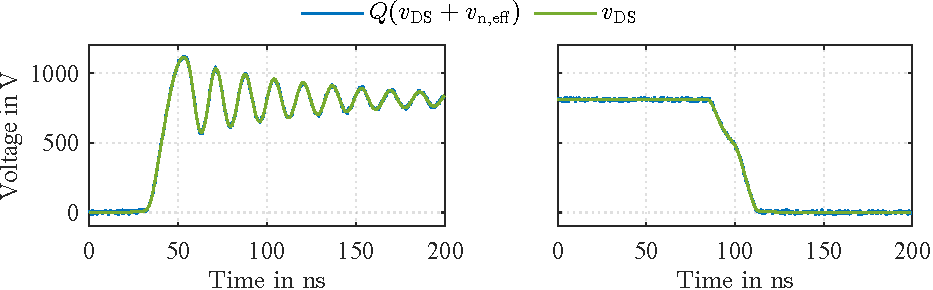
\includegraphics[scale = 1]{figures/3_Methods/Measurement_Limitation/DPT_TD_new.pdf}
		\caption{Time domain PSpice simulation of the drain-source voltage switching transient and the same signal contaminated with thermal and quantization noise.}
	\end{subfigure} %
	\par
	\vspace{1cm}
	\begin{subfigure}{\textwidth}
	\centering
		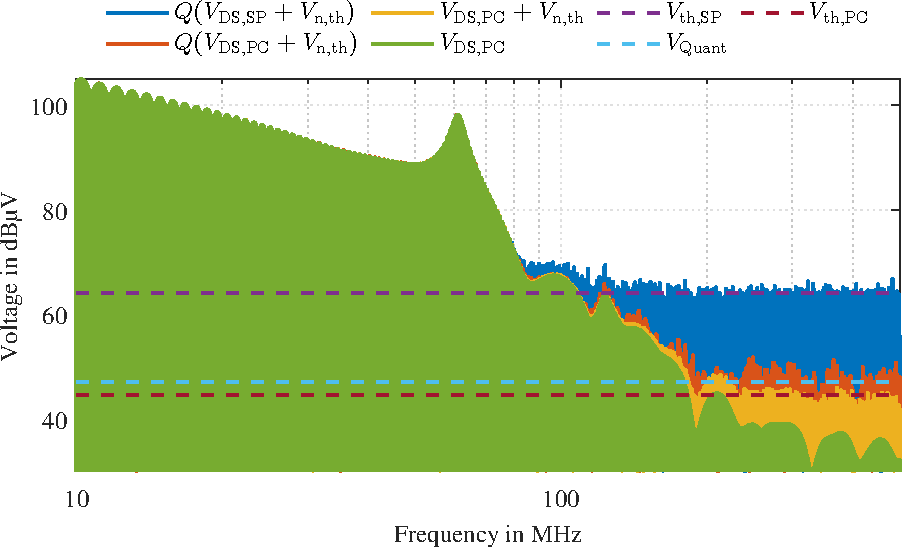
\includegraphics[scale = 1]{figures/3_Methods/Measurement_Limitation/DPT_FD_new.pdf}
		\caption{FFT of the simulated switching transient with and without thermal and quantization noise, shown for both a single pulse (SP) and a pulse chain (PC). Additionally, the calculated noise floors are added in dashed lines.}
	\end{subfigure}
	\caption{Limitation of measurement of switching transients due to quantization noise.}\label{fig:QuantNoise}
\end{figure}


For frequencies below \mbox{$\mi{f}{cut1} = \sfrac{1}{\pi \text{d} \mi{T}{sw}}$}, the spectrum is dominated by the DC component of the signal, \mbox{$\mi{V}{DS}(f=0) = \text{d}\cdot\mi{V}{DC}$}, where d is the duty cycle and \mi{T}{sw} is the switching period.
Above \mi{f}{cut1}, the spectrum decreases with \SI{-20}{dB/dec}. 
This range is mainly shaped by the switching frequency, modulation scheme, and operating point of the converter.

At frequencies above \mbox{$\mi{f}{cut2} = \sfrac{1}{\pi \mi{\uptau}{r}}$}, where \mi{\uptau}{r} denotes the switching transient time, the spectrum undergoes another transition. 
Idealized trapezoidal voltages then fall with \SI{-40}{dB/dec}, while real voltage transients can decay even faster, with \SIrange{-40}{-100}{dB/dec}.
In this region, the switching transient and, therefore, the semiconductor becomes the dominant factor shaping the spectrum.
% Above \mbox{$\mi{f}{cut2} = \sfrac{1}{\pi \mi{t}{r}}$} the switching transient and, thereby, the semiconductor is the dominating factor for the spectrum.

\subsection{Thermal Noise}

Figure~\ref{fig:QuantNoise} illustrates the resulting measurement challenge by comparing a simulated voltage transient and its spectrum with a quantized, noise-contaminated counterpart, for a zoomed view of the high-frequency region.

For calculation, thermal noise is taken from two sources: the oscilloscope datasheet gives \SI{1.61}{mV} at \SI{100}{mV/div}~\cite{tektronix_mso_2026}, and a conventional differential probe contributes \SI{55}{mV} at a divider ratio of \mti{a}{probe}~=~250~\cite{pmk_gmbh_datasheet_2017}.
The effective noise referred to the high-voltage side is then calculated as

\begin{equation}
	\mi{v}{n,th} = \mti{a}{probe}\cdot (\mi{v}{n,th,osci} + \mi{v}{n,th,probe}) 
\end{equation}

To express this noise in an amplitude-frequency plot, the thermal-noise density must be scaled by the FFT-bin width.

\begin{equation}
	\mi{V}{th} = \sqrt{\frac{\mi{V}{n,th,RMS}^2}{\Delta \mi{f}{FFT}} \cdot {\Delta \mi{f}{bin}}},
	\label{eq:RMStoAmplitudePlot}
\end{equation}

Here, \mi{f}{FFT} follows the Nyquist sampling theorem and equals \mbox{$\mi{f}{s}/2$}, where \mi{f}{s} is the oscilloscope sampling frequency. 
The term $\Delta \mi{f}{bin}$ denotes the FFT-bin width.
In logarithmic form, this becomes
\begin{equation}
	\mi{V}{th}^{\mathrm{dBµV}} = 20 \cdot \log_{10}\left(\frac{\mi{V}{th}}{\SI{1}{\micro V}}\right)
\end{equation}



\subsection{Quantization Noise}

Thermal noise is only one part of the measurement limit. 
ADC quantization noise must also be considered.
For simplicity, the quantization process can be written as a rounding function that maps the input signal to the nearest quantization level:
\begin{equation}
	Q(\mi{v}{DS}) = \text{round}\left(\frac{\mi{v}{DS}}{q}\right) \cdot q,
\end{equation}

Here, $q$ is the ADC quantization step, calculated as
\begin{equation}
	q = \dfrac{\mi{V}{max}-\mi{V}{min}}{2^{\mti{N}{ENOB}}}.
\end{equation}

The effective number of bits (ENOB) is typically lower than the nominal ADC resolution (\mi{N}{ADC}) because of non-idealities in the sampling process, such as jitter, thermal noise, and other error sources. It also decreases with frequency~\cite{tektronix_mso_2026}.

Assuming a uniform distribution of the quantization error, the quantization noise is calculated as~\cite{silicon_laboratories_an118_2013}
\begin{equation}
	\mi{V}{quant,RMS} = \sqrt{\frac{q^2}{12}}
\end{equation}

Using Eq.~\ref{eq:RMStoAmplitudePlot}, the quantization noise can then be transformed to the amplitude-frequency plot.

% \begin{equation}
% 	\mi{V}{quant,lin} = \frac{Q}{\sqrt{12}}\cdot\sqrt{\frac{2}{\mti{N}{FFT}}}
% \end{equation}


Figure~\ref{fig:QuantNoise} shows the spectrum of a quantized, noise-contaminated single-pulse signal, $Q(\mi{V}{DS,SP}+\mi{V}{n,th})$.
The single pulse represents a double-pulse test, which is commonly used for characterizing power semiconductor devices.

It can be clearly seen that above the resonance frequency at \SI{62}{MHz}, the signal drops below the noise floor at \SI{80}{MHz}, making it impossible to extract meaningful information about emitted noise.


This onset of the noise floor is expected and occurs slightly above the resonance frequency defined by MOSFET output capacitance and commutation-loop inductance, which is typically around \SIrange{10}{50}{MHz} for modules and \SIrange{80}{120}{MHz} for discrete devices, and therefore much lower than the probe bandwidth.
Hence, the limitation is not in the resolution or bandwidth of the probes (\SIrange{200}{1000}{MHz}), but in the noise of the measurement system.
Therefore, measuring the EMC-relevant frequency band of \SIrange{10}{400}{MHz} for SiC MOSFETs requires a measurement environment that overcomes these noise limitations.

It should be emphasized that these high-frequency voltage components are primarily relevant for EMC analysis.
For conventional metrics such as overvoltage, switching energy, and d$v$/d$t$, these components are too small to have a significant impact.


An exemplary calculation can be done with the spectra formulation from graphical analysis of a symmetric trapezoidal pulse \cite{costa_graphical_2005}.

\begin{equation}
\mi{V}{DS}(f) = d\,\mi{V}{DC}\,\text{sinc}(\pi f d \mi{T}{sw})\,\text{sinc}(\pi f \mi{\uptau}{r})
\end{equation}
 
\begin{align}
	\mi{V}{DS}(f) &= \text{d}\mi{V}{DC}\cdot\text{sinc}(\pi f \text{d} \mi{T}{sw})\cdot\text{sinc}(\pi f \mi{\uptau}{r})\\
	 &\le
 	\left\{
	\begin{array}{lllll}
		\text{d}\mi{V}{DC} 										 &\text{, for } \SI{0}{Hz} 							&\le f <&\dfrac{1}{\pi \text{d} \mi{T}{sw}} \\[6pt]
		\dfrac{\mi{V}{DC}}{\pi f \mi{T}{sw}} 					 &\text{, for } \dfrac{1}{\pi \text{d} \mi{T}{sw}}  &\le f <&\dfrac{1}{\pi \mi{\uptau}{r}} \\[6pt]
		\dfrac{\mi{V}{DC}}{\pi^{2} f^{2}\mi{T}{sw}\mi{\uptau}{r}}&\text{, for } \dfrac{1}{\pi \mi{\uptau}{r}}       &\le f  & \\[6pt]
	\end{array}
	\right.
\end{align}


To understand the root cause of this an exemplary calculation can be performed.
According to \cite{bi_prediction_2019}, the spectrum of an asymmetric first-order hold element for frequencies above the equivalent frequency of the rise time can be expressed as:

\begin{equation}
\mi{V}{DS}(f) = 
\dfrac{\mi{V}{DC}\mi{f}{sw}}{\uppi^2 f^2} (\dfrac{1}{\mi{\tau}{r}}+\dfrac{1}{\mi{\tau}{f}}), \quad \text{ for } f > \dfrac{1}{\uppi~\mathrm{min}(\mi{\tau}{r},\mi{\tau}{f})} 
\end{equation}

{\small
\begin{align}
\mi{V}{DS}(f) &= \begin{cases}
\dfrac{\mi{V}{DC}}{\uppi} \cdot \mid \mathrm{e}^{-\mathrm{j}\uppi \sfrac{\tau_r}{T}} - \mathrm{e}^{-\mathrm{j}\uppi (\sfrac{\mi{\tau}{r}}{T}+2\mathrm{D})} \mid & \text{, for }  0 \leq f \leq \dfrac{2}{T}\dfrac{\mathrm{e}^{\mathrm{j}\uppi\sfrac{\tau_r}{T}}}{\mid 1-\mathrm{e}^{-\mathrm{j}2\uppi  \mathrm{D}}\mid} \\
\dfrac{2\mi{V}{DC}\mi{f}{sw}}{\uppi f} & \text{, for } \dfrac{2}{T}\dfrac{\mathrm{e}^{\mathrm{j}\uppi\sfrac{\mi{\tau}{r}}{T}}}{\mid 1-\mathrm{e}^{-\mathrm{j}2\uppi \mathrm{D}}\mid} < f \leq \dfrac{1}{\uppi~ \mathrm{max}(\mi{\tau}{r},\mi{\tau}{f})} \\
\dfrac{\mi{V}{DC}\mi{f}{sw}}{\uppi f}(1+\dfrac{1}{\uppi f \mi{\tau}{f}}) & \text{, for } \dfrac{1}{\uppi~\mathrm{max}(\mi{\tau}{r},\mi{\tau}{f})} < f \leq \dfrac{1}{\uppi~\mathrm{min}(\mi{\tau}{r},\mi{\tau}{f})} \\
\dfrac{\mi{V}{DC}\mi{f}{sw}}{\uppi^2 f^2} (\dfrac{1}{\mi{\tau}{r}}+\dfrac{1}{\mi{\tau}{f}}) & \text{, for } \dfrac{1}{\uppi~\mathrm{min}(\mi{\tau}{r},\mi{\tau}{f})} < f \\
\end{cases} 
\end{align}
}

Now, lets assume some value as: \mi{V}{DC}~=~\SI{800}{V}, d~=~0.5, \mi{f}{sw}~=~\SI{25}{kHz}, \mi{\tau}{r}~=~\SI{20}{ns} and \mi{\tau}{f}~=~\SI{50}{ns}. As a result
\begin{equation}
	\mi{V}{DS}(f=\SI{100}{MHz}) = \SI{14.2}{mV}
\end{equation}

A classical probe with an attenuation of 250 is used, which results in an ADC input voltage 
\begin{equation}
	\mi{v}{ADC,in} = \dfrac{\mi{v}{meas}}{\mti{a}{probe}} = \dfrac{\SI{14.2}{mV}}{250} = \SI{57}{\upmu V}
\end{equation}

The problem is evident when the minimum voltage increment of the oscilloscopes ADC is calculated, with an ADC, with an effective number of bits (ENOB) of 14
\begin{equation}
	\mi{v}{ADC,min} = \dfrac{\mi{V}{max}-\mi{V}{min}}{\mti{a}{probe}\cdot 2^{\mti{N}{bit}}} = \dfrac{\SI{1200}{V} - (\SI{-150}{V})}{250\cdot 2^{14}} = \SI{330}{\upmu V}.
\end{equation} 

The two values are of the same order of magnitude, which makes it for the ADC impossible to sample this voltage components.
Additional to the quantization noise some thermal noise adds to the noise floor, creating a higher, effective noise floor, as can be seen in Fig. \ref{fig:QuantNoise}.
\begin{equation}
	\mi{v}{noise,eff} = \mi{v}{noise,quant} + \mi{v}{noise,therm}
\end{equation}
%!TeX root = main.tex
%!encoding = UTF-8 Unicode

\section{Oversampling and Averaging}
The previous section explains the challenges to measure high-frequency components of a signal.
Firstly, classical digital noise reduction can be applied, which address the thermal noise \mi{v}{noise,therm}: Oversampling and averaging.

By oversampling and averaging afterwards, the effective number of bits (ENOB) can be increased by \cite{silicon_laboratories_an118_2013}.

\begin{equation}
	\mti{N}{ENOB} = \mti{N}{ADC} + 0.5\cdot \log_2(\frac{\mi{f}{s}}{2\mi{f}{max}})
\end{equation}

Here \mi{N}{ADC} is the nominal ADC resolution, \mi{f}{s} is the sampling frequency of the oscilloscope and \mi{f}{max} the maximum frequency of interest.
Furthermore, the factor of 2 in the denumerator is due to the nyquist sampling theorem.
This can be done internally in the oscilloscope.

As this cannot be pushed limitless due to hardware-restrictions of the maximum sampling speed of modern oscilloscopes, the number of signal points can be increased by not measuring one single pulse, but a pulse chain of $M$ pulses.
This further increases the ENOB to \cite{kragl_active_2025}

\begin{equation}
	\mti{N}{ENOB} = \mti{N}{ADC} + 0.5\cdot \log_2(\frac{\mi{f}{s}}{2\mi{f}{max}}) + 0.5\log_2(M)
\end{equation}

These gains are realized only if the dominant noise is random, uncorrelated with the signal, and greater than the quantization step \cite{silicon_laboraties_an118_2013}. 
As discussed above, in power electronics the high‑frequency voltage components often fall below or near the ADC quantization level; therefore oversampling and averaging alone are insufficient and must be combined with a high‑pass measurement method introduced next.

%!TeX root = main.tex
%!encoding = UTF-8 Unicode

\section{High-Pass Measurement}
To overcome quantization-noise limitations, a high-pass filter is applied. 
The key principle is to compensate for the natural \SI{-40}{dB/dec} roll-off of the switching spectrum (Section~II-A) using a high-pass transfer function with a \SI{+40}{dB/dec} slope. 
This flattens the signal at the ADC input, pushing it well above the quantization noise floor \mi{V}{Quant} and extending the usable measurement range. 
The resulting filtered signal is then compensated in post-processing to recover the original voltage spectrum, as visualized in Fig.~\ref{fig:QuantNoise_wHP}.

\begin{figure}[ht]
	\begin{subfigure}{0.48\textwidth}
	\centering
		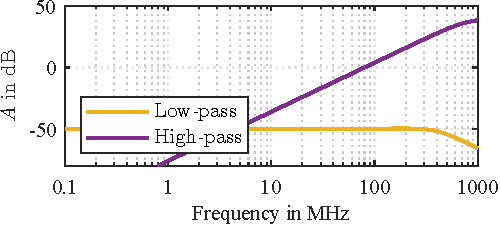
\includegraphics[scale = 1]{figures/3_Methods/Highpass/TF_FD.pdf}
		\caption{Transfer function of conventional low-pass measurement and second order high-pass.}
	\end{subfigure}%
	\hfill
	\begin{subfigure}{0.48\textwidth}
		\centering
		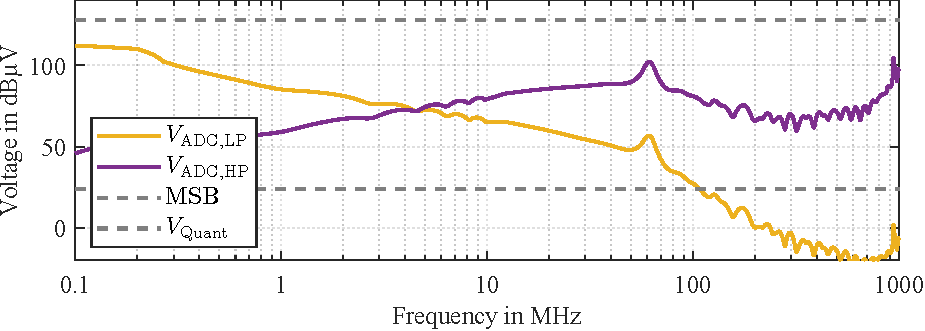
\includegraphics[scale = 1]{figures/3_Methods/Highpass/ADC_sig.pdf}
		\caption{Effective voltage spectrum of low-pass and high-pass measurements at the oscilloscope input with the respective quantization-noise floor.}
	\end{subfigure}
	\caption{Measurement principle of a high-pass measurement for EMC-relevant frequency components of a transient signal.}\label{fig:QuantNoise_wHP}
\end{figure}

To compensate for the transfer function and reconstruct the original signal, the high-pass probe is modeled as a linear time-invariant (LTI) system with impulse response $\mi{a}{HP}(t)$ and frequency-domain transfer function $\mi{A}{HP}(f)$.
At the oscilloscope input, the measured signal is the convolution of the drain-source voltage with the probe response:
\begin{equation}
	\mi{v}{DS,HP,raw}(t) = \mi{a}{HP}(t) \ast \mi{v}{DS}(t),
\end{equation}

which in the frequency domain becomes a multiplication:
\begin{equation}
	\mi{V}{DS,HP,raw}(f) = \mi{A}{HP}(f) \cdot \mi{V}{DS}(f).
\end{equation}

To recover the original drain-source voltage spectrum, the measured signal is compensated by the transfer function:
\begin{equation}
	\mi{V}{DS,HP,comp}(f) = \frac{\mathcal{F}\{\mi{v}{DS,HP,raw}(t)\}}{\mi{A}{HP}(f)} = \frac{\mi{V}{DS,HP,raw}(f)}{\mi{A}{HP}(f)}.
	\label{eq:HP_comp}
\end{equation}

In logarithmic representation, this division becomes a simple subtraction of the probe gain curve $\mi{A}{HP}(f)$:
\begin{equation}
	\mi{V}{DS,HP,comp}^{\text{dB}\upmu\text{V}} = \mi{V}{DS,HP,raw}^{\text{dB}\upmu\text{V}} - \mi{A}{HP}^{\text{dB}}.
\end{equation}

As a result, the measurement is no longer limited by the onset of the noise floor, but primarily by the bandwidth of the probe and additional noise introduced by the high-pass filter.


%!TeX root = main.tex
%!encoding = UTF-8 Unicode

\section{Switching Event Separation}
In the analysis of the switching behavior of power electronics it is common practice to analyze the four switching events separately - active-off/passive-on and active-on/passive-off \cite{fritz_toward_2020}. 
Here, the active device is the switch, which initiates the switching transient while the passive switch is turned off and the body diode operates during the commutation process.
This separated analysis is also desirable for the EMC analysis to identify the switching event that is dominating the frequency spectrum for the respective frequency band of interest.
This is enabled by-and one of the main advantages-of the measurement directly at the semiconductor ports. 
Conventional EMC measurements at LISNs or antennas can only measure the conglomerated noise of all switching events and noise sources in the system.

However, to achieve this separated analysis in the frequency domain, a method introduced in \cite{kragl_impact_2024} must be used, called snap-and-mirror function.

\begin{figure}
	\begin{subfigure}[t]{0.48\textwidth}
		\centering
		\import{./figures/}{3_Methods/SnapNMirror/DPT_TD.tex}
		\subcaption{Active and passive switching signals in time domain.}
	\end{subfigure}
	\hfill
	\begin{subfigure}[t]{0.48\textwidth}
		\centering
		\import{./figures/}{3_Methods/SnapNMirror/DPT_FD.tex}
		\subcaption{Spectrum of active and passive switch.}
	\end{subfigure}
	
	\begin{subfigure}[t]{0.48\textwidth}
		\centering
		\import{./figures/}{3_Methods/SnapNMirror/Snapped_TD.tex}
		\subcaption{Snapped and mirrored time domain signals.}
	\end{subfigure}
	\hfill
	\begin{subfigure}[t]{0.48\textwidth}
		\centering
		\import{./figures/}{3_Methods/SnapNMirror/Snapped_FD.tex}
		\subcaption{Spectrum of snapped and mirrored signals.}
	\end{subfigure}
	\label{fig:SnM_snapped_FD}
	\vspace{1cm}
\end{figure}

% \begin{figure}[h!]
% 	\centering\import{./figures/}{2_SnapNMirror/DPT_TD.tex}
% 	\caption{Principle functionality of snap and mirror function for the separated EMC analysis of all four switching events.}
% 	\label{fig:SnapNMirror}
% \end{figure}



\begin{figure}[h!]
	\centering\import{./figures/}{Snap_n_Mirror_vertical_v3_tex.pdf_tex}
	\caption{Principle functionality of snap and mirror function for the separated EMC analysis of all four switching events.}
	\label{fig:SnapNMirror}
\end{figure}

This function identifies the mid-points of each switching cycle \mi{t}{mid,n} and mirrors them around this axis, which can be formulated as

\begin{equation}
	\small 
	\mathrm{s}_\mathrm{new}(t) = 
	\begin{cases}
		s(t) 					 		& \text{, for } \mi{t}{mid,n}~~~   < t < \mi{t}{mid,n+1} \\
		s(-t + 2\cdot\mi{t}{mid,n+1}) 	& \text{, for } \mi{t}{mid,n+1} < t < \mi{t}{mid,n+2} \\
		s(t) 					 		& \text{, for } \mi{t}{mid,n+2} < t < \mi{t}{mid,n+3} \\
		s(-t + 2\cdot\mi{t}{mid,n+3}) 	& \text{, for } \mi{t}{mid,n+3} < t < \mi{t}{mid,n+4} \\
		...\\
	\end{cases}
	\label{eq:snap}
\end{equation}

This is done for both the turn-on and turn-off event for both the active and the passive switch, thereby creating four artificial signals out of the two measured voltages of active and passive switch.

Because only the signal amplitude in the frequency domain is analyzed this is a valid operation since the mirroring and the time shift of a signal has only influence on the phase of the fourier transform.

\begin{equation}
	\mathcal{F}\{s(-t)\} = S(-f) = S^\ast(f)
\end{equation}

\begin{equation}
	\mathcal{F}\{s(t-\mi{t}{0})\} = S(f)e^{-j\omega \mi{t}{0}}
\end{equation}









	%!TeX root = main.tex
%!encoding = UTF-8 Unicode

\chapter{Dual-Channel Differential Active Voltage Probe}

%!TeX root = main.tex
%!encoding = UTF-8 Unicode

\section{Measurement-Driven Requirements for the Active Voltage Probe}
\label{sec:VoltageRequirements}

Prior to designing the dual-channel differential active voltage probe, its requirements are established. 
These requirements are specifically tailored for discrete SiC-MOSFETs, the primary focus of this work. 
Should the target devices change to SiC power modules or GaN devices, some modifications are necessary. 
The requirements are defined in accordance with the measurement limitations introduced in section \ref{sec:MeasurementLimitation}. 

\subsubsection*{Small Signal Response}
The small signal response of the probe is characterized by its bandwidth, which must exceed the maximum frequency of interest \mi{f}{interest,max} relevant to the measurements.
As discussed in section \ref{ch:methods}, this maximum frequency differs between low-pass and high-pass measurements.
For low-pass measurements, the bandwidth requirement corresponds to the maximum frequency of voltage components still above the noise floor.
For high-pass measurements, the maximum frequency of interest is set to \SI{500}{MHz}, which represents the point at which EMC-related issues transition from being caused by semiconductor switching events to those arising from digital signal sources, such as microcontroller and FPGA clock signals.

\subsubsection*{Large Signal Response}
The large signal response of the probe is characterized by its maximum input voltage, which must exceed the maximum voltage of interest \mi{V}{interest,max} relevant to the measurements.
Since the target of this work are \SI{1200}{V} SiC-MOSFETs, the maximum voltage of interest is set to \SI{1200}{V}.
Furthermore, the minimal rise time is determined by the minimal rise time possible in a given $LC$ resonant tank.
The stray inductance of the setup is around \SI{25}{nH}, and the output capacitance of the smallest investigated MOSFET, which is a \SI{30}{A} device is \SI{74}{pF}.
The rise time of an underdamped LC resonant tank is given by:

\begin{equation}
t_r = \frac{\pi}{\omega_n\sqrt{1-\zeta^2}} - \frac{\arcsin(\zeta)}{\omega_n\sqrt{1-\zeta^2}}
\end{equation}

where the natural frequency is $\omega_n = \frac{1}{\sqrt{LC}}$ and the damping ratio is $\zeta = \frac{R}{2}\sqrt{\frac{C}{L}}$ for a series RLC circuit.

For lightly damped systems ($\zeta \ll 1$), this simplifies to:

\begin{equation}
t_r \approx 1.8\cdot\sqrt{LC}
\end{equation}

This results in a minimal rise time of approximately \SI{2.5}{ns} for the given LC parameters.
However, this value represents a purely passive response that assumes an infinitely fast switch, a condition that is typically observed only during uncontrolled diode snap-off events.
In classical operation, the switching transient is predominantly determined by the gate-drive and is typically in the range of several tens of nanoseconds.


\subsubsection*{Parasitic Coupling}
As in any practical measurement setup, parasitic coupling can occur between the probe and the DUT.
For the proposed voltage probe, the dominant mechanism is capacitive coupling from the switching-node potential into the sensitive amplification stage.
Because this influence depends strongly on layout- and setup-specific conditions, it cannot be represented by a single precise quantitative requirement.
Therefore, the final measurement results must be validated by cross-checking against a trusted reference, typically a conventional passive voltage probe.

\subsubsection*{Transmission Line Effects}
In high-frequency measurements, transmission line effects can significantly impact the accuracy of the voltage probe.
This is explicitly a problem for voltage measurement, since the source impedance of the MOSFET is changing over the switching event and the load impedance of the probe is very high in range of ${M\Omega}$.
The transmission line impedance of the connection is normally in the range of \SI{50}{\Omega} to \SI{75}{\Omega}, which is significantly lower than the input impedance of the probe.
Hence, to avoid reflections and signal distortion, the connection between the probe and the DUT must be as short as possible, but maximally

\begin{align}
    \mi{l}{max} \leq \frac{\lambda_\mathrm{min}}{10} &= \frac{c_0}{10\cdot\mi{f}{max}\sqrt{\epsilon_r}} \\
                                                    &= \frac{c_0}{10\cdot \SI{500}{MHz}\cdot \sqrt{4.25}} \\
                                                    &= \SI{2.9}{cm}
\end{align}

This allowable distance is too short to be implemented in a practically useful setup with a cable connection.
Therefore, the probe must be designed for a direct connection to the drain and source terminals of the DUT.
%!TeX root = main.tex
%!encoding = UTF-8 Unicode

\section{Design}

\subsection{Frequency compensated voltage divider}
\subsection{Amplification}

For the measurement of the drain-source voltage, a dual-channel differential active voltage probe is utilized. 
This probe enables simultaneous measurement of the drain-source voltages across both switching devices. The probe is connected directly to the respective drain and source terminals, without the use of any cables, which change their impedance and transfer function in dependence of their positioning.
Furthermore this approach minimizes parasitic effects. 

\begin{figure}[h]
	\centering
	\import{./figures/}{SchematicOverviewEMEProbe.pdf_tex}
	\caption{Schematic overview of probe functionality.}
	\label{fig:OverviewEMEProbe}
\end{figure}

In contrast to conventional differential probes the signal is split after the unity gain amplifier to a second channel, which has a 2nd order high-pass characteristic.
The probe is a new version of the design of \cite{kragl_active_2025} incorporating an additional shielding layer in a now 6-layer PCB.
Furthermore, the HV PCB capacitor can be now trimmed by adding or removing the effective area of the outer capacitor side.
The new design was verified with the methods introduced in \cite{kragl_active_2025} for both large signal as small signal response.
The VNA measurement results are additionally shown in \fref{fig:VNA_LP} anf \fref{fig:VNA_HP}.


As was explained in \cite{kragl_active_2025} each probe is verified with 3 measurements: VNA Small signal, Pulse Generator Large signal, and i-situ measuremnt in parallel with commercial measurement (for lowpass measurements - \SI{80}{mR} passive shunt and \SI{10}{MR} passive probe). 
the last is necessary for the verification of not having any parasitic capacitive or inductive couplings into the measurement path.


% \begin{figure}[ht]
% 	\centering
% 	\input{"VNA_Probe_LP.tex"}
% 	\caption{VNA measurement of low pass.}
% 	\label{fig:VNA_LP1}
% \end{figure}

\begin{figure}[ht]
	\centering
	\import{./figures/}{VNA_LP.tex}
	\caption{VNA measurement of low pass.}
	\label{fig:VNA_LP}
\end{figure}

The voltage gain \mti{a}{probe} of the probe can be calculated from the S-parameter measurement as 
\begin{align}
	\mti{a}{probe} 	&= \frac{\mi{v}{out}}{\mi{v}{HV+}-\mi{v}{HV-}} \\
					&= \frac{\mti{S}{21}}{1 + \mti{S}{11}}.
\end{align}

Since \mti{S}{11} remains mostly flat at \SI{0}{dB} due to the high-impedance input of the probe, the primary parameter of interest for the voltage gain is \mti{S}{21}.

The low-pass signal exhibits a bandwidth of approximately \SI{250}{MHz} before the gain begins to drop, a limitation attributed to the characteristics of the operational amplifier employed in the output stage.

% \begin{figure}[ht]
% 	\centering
% 	\input{"VNA_Probe_HP.tex"}
% 	\caption{VNA measurement of high pass.}
% 	\label{fig:VNA_HP}
% \end{figure}

\begin{figure}[ht]
	\centering
	\import{./figures/}{VNA_HP.tex}
	\caption{VNA measurement of high pass.}
	\label{fig:VNA_HP}
\end{figure}

Considering the high pass transfer function the constant rise of gain over frequency was achieved with an additional input inductance in front of the unity gain amplifier. 
This compensates capacitive input behavior of the used 

%!TeX root = main.tex
%!encoding = UTF-8 Unicode

\section{Verification}

\subsection{Small-Signal}
The updated probe was validated using the methodology of~\cite{kragl_active_2025}: large-signal verification with a \SI{50}{\ohm} pulse generator, small-signal characterization with a vector network analyzer (VNA), and low-pass cross-verification against a standard passive probe to exclude unintended capacitive or inductive coupling into the active measurement path.
The VNA results for the low-pass and high-pass channels are shown in \fref{fig:VNA_LP} and \fref{fig:VNA_HP}, respectively.

\begin{figure}[ht]
	\centering
	% This file was created by matlab2tikz.
%
%The latest updates can be retrieved from
%  http://www.mathworks.com/matlabcentral/fileexchange/22022-matlab2tikz-matlab2tikz
%where you can also make suggestions and rate matlab2tikz.
%
\definecolor{mycolor1}{rgb}{0.00000,0.44700,0.74100}%
\definecolor{mycolor2}{rgb}{0.85000,0.32500,0.09800}%
\definecolor{mycolor3}{rgb}{0.92900,0.69400,0.12500}%
\definecolor{mycolor4}{rgb}{0.49400,0.18400,0.55600}%
%
\begin{tikzpicture}

\begin{axis}[%
width=5.492in,
height=1.726in,
at={(0.921in,0.459in)},
scale only axis,
xmode=log,
xmin=0.1,
xmax=1000,
xtick={0.1,1,10,100,1000},
xticklabels={{0.1},{1},{10},{100},{1000}},
xminorticks=true,
xlabel style={font=\color{white!15!black}},
xlabel={Frequency in MHz},
ymin=-120,
ymax=0,
ylabel style={font=\color{white!15!black}},
ylabel={Magnitude in dB},
axis background/.style={fill=white},
xmajorgrids,
xminorgrids,
ymajorgrids,
grid style={dotted},
legend style={at={(0.03,0.97)}, anchor=north west, legend cell align=left, align=left, draw=white!15!black}
]
\addplot [color=mycolor1, line width=1.5pt]
  table[row sep=crcr]{%
0.1	-0.07846622336\\
0.103527468	-0.07281316743\\
0.111287897	-0.0604819558\\
0.1218703	-0.05118142218\\
0.169625017	-0.01909939471\\
0.177410572	-0.01626313434\\
0.213043601	-0.0123325037\\
0.221095909	-0.009386099722\\
0.235858474	-0.007056501781\\
0.251963091	-0.00397916227\\
0.261582765	-0.006170257478\\
0.27819181	-0.00706560105\\
0.307719002	-0.002850289133\\
0.367338544	-0.003982124183\\
0.382612797	-0.004638276902\\
0.397887049	-0.004522527786\\
0.423344138	-0.00870968907\\
0.458984061	-0.01214321664\\
0.515158441	-0.01780833359\\
0.550264191	-0.02110193266\\
0.574838217	-0.02303635007\\
0.581859367	-0.01501449397\\
0.638028568	-0.0174308464\\
0.747210132	-0.02280914783\\
0.776266149	-0.0240619522\\
0.800479497	-0.02371164862\\
0.986657469	-0.02360528924\\
1.013369958	-0.02362429898\\
1.093507426	-0.023336047\\
1.19367926	-0.02175778245\\
1.329199574	-0.01970685733\\
1.356748752	-0.01957737716\\
1.779169483	-0.01774601711\\
1.815229447	-0.01677193687\\
2.119251578	-0.01278797739\\
2.283930232	-0.01208934467\\
2.461276475	-0.01021458481\\
2.825489325	-0.007963133831\\
2.982708678	-0.008340162023\\
3.789233904	-0.006032796791\\
4.413787719	-0.004053784524\\
4.557915522	-0.004543222154\\
5.245370812	-0.003421718683\\
5.974367849	-0.004042798948\\
7.665165585	-0.004361392422\\
8.396292216	-0.004376814852\\
16.75449209	-0.01301079408\\
20.1702834	-0.01778258931\\
21.96325333	-0.01961585502\\
26.59592024	-0.02583681854\\
31.21277638	-0.02388283718\\
34.73154665	-0.022885865\\
45.88317121	-0.02382433264\\
56.2013919	-0.03600572225\\
60.9439864	-0.04418073353\\
63.10057567	-0.0466067823\\
80.78460774	-0.0709658106\\
87.28297277	-0.08771253368\\
89.66215094	-0.09608055286\\
98.58406908	-0.1228602446\\
103.3424254	-0.141600567\\
125.7477651	-0.235706467\\
129.0193635	-0.244406597\\
141.2878576	-0.2840949975\\
147.0131548	-0.2973470867\\
157.6458497	-0.3133748837\\
161.675471	-0.3101500341\\
167.3167369	-0.2959494373\\
175.2145091	-0.2691481874\\
181.9840281	-0.2481186512\\
193.2665598	-0.224600721\\
218.0881296	-0.2130461436\\
226.7613334	-0.2140140333\\
245.4318936	-0.2297653559\\
254.7671736	-0.2446945034\\
260.9906937	-0.2482738101\\
274.9936138	-0.2644505731\\
281.2171338	-0.2767142849\\
295.2200539	-0.314594602\\
313.9919762	-0.388701852\\
326.8695461	-0.460069285\\
341.8933777	-0.5385392456\\
361.2097326	-0.6270667817\\
363.3559942	-0.6296909458\\
376.2335641	-0.6051718185\\
386.9648724	-0.5690876868\\
395.549919	-0.5623482225\\
404.1349656	-0.5482955845\\
410.5737506	-0.5422699532\\
425.4457377	-0.5235677325\\
431.3651992	-0.5166038256\\
452.0833145	-0.5506225483\\
458.0027759	-0.5680771798\\
469.8416989	-0.6196249933\\
484.6403527	-0.6628363857\\
505.3584679	-0.687656716\\
517.1973909	-0.6864404092\\
523.1168524	-0.6870766127\\
531.9960446	-0.6783757616\\
543.8349676	-0.6831053609\\
570.4725443	-0.7274892639\\
576.8889099	-0.7332441373\\
585.0287378	-0.7445589042\\
593.1685657	-0.7527488083\\
617.5880494	-0.785006949\\
629.7977913	-0.7893198389\\
642.0075331	-0.7977763436\\
650.147361	-0.8082804887\\
662.3571029	-0.8134745731\\
666.4270168	-0.8169590603\\
674.5668447	-0.8420836198\\
698.9863284	-0.9300929756\\
711.1960703	-0.9631653857\\
719.3358982	-0.9825572794\\
727.4757261	-0.9876890696\\
776.3146935	-0.9514121656\\
780.3846075	-0.9535602494\\
788.5244354	-0.9470000011\\
798.8918907	-0.9410285573\\
826.9631436	-0.9749290544\\
838.1916447	-0.9698013576\\
855.0343964	-0.9460258091\\
860.648647	-0.9436667998\\
871.8771481	-0.9324516207\\
883.1056493	-0.935251179\\
894.3341504	-0.9505063803\\
928.0196538	-1.044210905\\
950.4766561	-1.061124941\\
967.3194078	-1.058622167\\
978.547909	-1.055705716\\
995.3906607	-1.065997586\\
1001.004911	-1.073095926\\
};
\addlegendentry{$\mathrm{S}_\mathrm{11}$}

\addplot [color=mycolor2, line width=1.5pt]
  table[row sep=crcr]{%
0.1	-112.8328954\\
0.100705494	-114.9842329\\
0.101410987	-101.4172326\\
0.102116481	-105.7286472\\
0.103527468	-96.24597605\\
0.104232961	-113.3339689\\
0.104938455	-100.5300715\\
0.105643948	-101.1989067\\
0.106349442	-96.4939973\\
0.108465922	-119.3674632\\
0.109876909	-98.80374902\\
0.110582403	-102.4430964\\
0.112698884	-98.48694328\\
0.113404377	-99.15804426\\
0.114109871	-97.27431293\\
0.115520858	-107.4046829\\
0.116226351	-100.2366247\\
0.116931845	-107.1522209\\
0.118342832	-96.04198044\\
0.119048325	-96.6225612\\
0.119753819	-95.70259395\\
0.120459312	-108.8167114\\
0.122575793	-98.63767665\\
0.123281287	-104.5729089\\
0.124692274	-100.5167641\\
0.125397767	-91.43354558\\
0.126808754	-108.9202416\\
0.128219741	-101.5818604\\
0.130336222	-113.0873824\\
0.131041715	-111.4814438\\
0.131747209	-105.33938\\
0.133158196	-108.2095469\\
0.135274677	-105.4934482\\
0.13598017	-118.5143202\\
0.137509601	-103.5914488\\
0.138482796	-106.619694\\
0.13945599	-105.4333694\\
0.140429185	-106.3237623\\
0.141402379	-112.9210948\\
0.143348768	-101.8896779\\
0.144321962	-110.4065857\\
0.146268351	-100.3478421\\
0.147241545	-106.5767639\\
0.14821474	-104.9026172\\
0.149187934	-100.3068082\\
0.151134323	-116.9927581\\
0.153080712	-99.25272924\\
0.154053906	-106.2848012\\
0.156000295	-104.7976404\\
0.156973489	-99.66875171\\
0.157946684	-99.91704754\\
0.159893073	-112.5703093\\
0.160866267	-108.9718097\\
0.162812656	-99.63823189\\
0.16378585	-99.54836034\\
0.164759045	-106.0811649\\
0.165732239	-94.4435988\\
0.167678628	-114.0096961\\
0.169625017	-102.1188996\\
0.171571405	-119.0802996\\
0.173517794	-107.6248561\\
0.174490989	-109.1773506\\
0.176437377	-104.707887\\
0.180330155	-112.955784\\
0.181303349	-97.49860134\\
0.183249738	-110.1750978\\
0.184222933	-107.5992622\\
0.186169321	-125.8842688\\
0.187142516	-104.6799865\\
0.18811571	-109.0997917\\
0.189088905	-104.1144604\\
0.190228728	-125.0376478\\
0.191570779	-99.6624457\\
0.19291283	-105.1243279\\
0.194254882	-124.4491932\\
0.196938984	-105.8627296\\
0.198281036	-109.8091414\\
0.199623087	-107.9122293\\
0.200965139	-108.5528656\\
0.20230719	-106.4689384\\
0.204991293	-108.5077335\\
0.206333344	-105.9350775\\
0.207675395	-112.5765818\\
0.209017447	-103.6283121\\
0.21170155	-112.1175502\\
0.213043601	-119.4335062\\
0.215727704	-111.5976296\\
0.217069755	-107.7363338\\
0.218411806	-112.7243914\\
0.219753858	-110.8545182\\
0.221095909	-119.9175259\\
0.225122063	-107.3717081\\
0.227806166	-118.7726695\\
0.229148217	-108.3554652\\
0.23183232	-116.403699\\
0.233174371	-110.1790395\\
0.234516423	-115.6598623\\
0.235858474	-108.2825623\\
0.237200526	-114.8740979\\
0.238542577	-108.1666603\\
0.239884628	-108.6285138\\
0.242568731	-116.7244955\\
0.243910782	-116.0330285\\
0.245252834	-124.1077996\\
0.246594885	-111.3093472\\
0.247936937	-118.7405038\\
0.249278988	-118.6779519\\
0.250621039	-113.7370871\\
0.251963091	-117.3532473\\
0.253305142	-110.2518996\\
0.254647193	-126.8089115\\
0.255989245	-108.4841549\\
0.257331296	-113.9442428\\
0.258673347	-109.58563\\
0.260015399	-114.8746304\\
0.261582765	-106.7168005\\
0.263428214	-111.1327106\\
0.265273664	-127.7240831\\
0.267119113	-108.9062172\\
0.270810012	-112.0843905\\
0.272655462	-116.6029107\\
0.274500911	-109.1541697\\
0.276346361	-118.6153542\\
0.27819181	-116.7564544\\
0.28003726	-112.9818942\\
0.281882709	-124.1094129\\
0.289264507	-101.0699033\\
0.291109957	-123.4888539\\
0.296646305	-102.4356459\\
0.298491755	-107.4655628\\
0.302182654	-104.8141209\\
0.305873553	-109.3359443\\
0.307719002	-90.45869933\\
0.309564452	-115.5561017\\
0.311409901	-107.390332\\
0.3151008	-115.7380408\\
0.31694625	-97.78090175\\
0.318791699	-102.3122469\\
0.320637149	-114.3707506\\
0.324328048	-107.7618168\\
0.329864396	-124.8706773\\
0.331709845	-117.97451\\
0.333555295	-99.86435405\\
0.337246194	-113.5953344\\
0.342782542	-95.06492961\\
0.346473441	-107.3422452\\
0.348318891	-108.463775\\
0.35016434	-104.1846655\\
0.35200979	-123.6116553\\
0.355700689	-105.2710058\\
0.357546138	-112.4204911\\
0.362247126	-109.1561029\\
0.364792835	-121.0929008\\
0.367338544	-116.2098495\\
0.369884252	-123.0520519\\
0.372429961	-115.9759592\\
0.37497567	-118.0069635\\
0.377521379	-114.4895708\\
0.380067088	-116.2942204\\
0.382612797	-115.6520157\\
0.387704214	-111.8855269\\
0.390249923	-112.047096\\
0.392795632	-121.1566061\\
0.395341341	-109.8614113\\
0.400432758	-123.8868573\\
0.402978467	-115.5715003\\
0.405524176	-118.5659817\\
0.408069885	-106.980466\\
0.410615594	-129.5104323\\
0.413161302	-105.9257149\\
0.41825272	-115.1245261\\
0.420798429	-105.3928398\\
0.423344138	-110.0940324\\
0.425889847	-107.6421607\\
0.428435555	-108.4326321\\
0.430981264	-86.94101807\\
0.433526973	-106.9691979\\
0.438618391	-101.7699944\\
0.443709808	-109.2454959\\
0.446255517	-104.3122229\\
0.448801226	-120.7099236\\
0.453892644	-108.6591213\\
0.456438352	-109.7866878\\
0.458984061	-101.9791526\\
0.46152977	-110.6413792\\
0.466621188	-97.44757036\\
0.471712605	-104.6086613\\
0.474258314	-102.4272372\\
0.476804023	-114.1276678\\
0.479349732	-100.696936\\
0.481895441	-100.7234403\\
0.484441149	-113.6341373\\
0.489532567	-100.3997159\\
0.492078276	-114.0472349\\
0.494623985	-105.468175\\
0.50111614	-109.2139096\\
0.504626715	-103.9079216\\
0.50813729	-104.2907881\\
0.511647866	-128.3860625\\
0.518669016	-88.73584547\\
0.522179591	-103.76244\\
0.525690166	-100.3459898\\
0.529200741	-114.6025621\\
0.536221891	-99.1862114\\
0.539732466	-109.1011481\\
0.546753616	-101.003943\\
0.550264191	-109.56135\\
0.553774767	-99.72322335\\
0.560795917	-102.8251301\\
0.564306492	-99.83083671\\
0.567817067	-116.0747093\\
0.571327642	-85.0403188\\
0.574838217	-97.17466449\\
0.578348792	-91.82044194\\
0.581859367	-98.73792579\\
0.585369942	-94.13910478\\
0.588880517	-98.89843406\\
0.592391092	-96.61737616\\
0.595901667	-113.947912\\
0.602922818	-82.90288892\\
0.613454543	-101.1156397\\
0.616965118	-89.07822109\\
0.623986268	-97.68894265\\
0.627496843	-111.961252\\
0.631007418	-110.2739545\\
0.634517993	-103.6306636\\
0.638028568	-108.7866726\\
0.645049719	-104.3960024\\
0.648560294	-99.66699246\\
0.652070869	-115.2928295\\
0.659092019	-107.3922599\\
0.662602594	-115.6365343\\
0.666113169	-109.3724861\\
0.669623744	-113.2435962\\
0.673134319	-100.5533722\\
0.676644894	-108.3263185\\
0.680155469	-104.4418836\\
0.689098098	-109.519986\\
0.698783437	-126.1190794\\
0.708468776	-106.187503\\
0.713311446	-107.6768158\\
0.718154115	-115.7053114\\
0.722996785	-102.2591842\\
0.727839454	-109.5113889\\
0.732682124	-103.8151862\\
0.737524793	-110.5904237\\
0.747210132	-101.6647646\\
0.752052802	-106.9133398\\
0.756895471	-95.98572402\\
0.76658081	-106.1443185\\
0.77142348	-98.55140102\\
0.776266149	-129.0176678\\
0.785951488	-109.0566209\\
0.795636827	-117.8557973\\
0.800479497	-107.1183956\\
0.810164836	-120.969819\\
0.815007505	-105.9548356\\
0.819850175	-119.0067582\\
0.824692844	-113.7742136\\
0.829535514	-120.572235\\
0.839220853	-110.4795735\\
0.848906192	-116.5956021\\
0.853748861	-119.028136\\
0.858591531	-114.3976076\\
0.8634342	-120.945205\\
0.86827687	-107.4187693\\
0.873119539	-111.661346\\
0.877962209	-106.477655\\
0.882804878	-108.3790836\\
0.887647548	-104.0614134\\
0.897332887	-112.0799403\\
0.902175556	-124.5193502\\
0.907018226	-115.7526847\\
0.911860895	-118.4363654\\
0.916703565	-95.55347024\\
0.926388904	-111.4129401\\
0.931231573	-110.4687555\\
0.936074243	-108.0410775\\
0.946588735	-118.0826407\\
0.95994498	-101.9114485\\
0.973301224	-115.6397862\\
0.979979347	-114.7578888\\
0.986657469	-98.62105623\\
0.993335591	-102.8960819\\
1.000013714	-99.40940356\\
1.006691836	-108.160881\\
1.013369958	-107.6191816\\
1.02004808	-103.1703346\\
1.033404325	-108.5124669\\
1.04676057	-103.3086914\\
1.053438692	-99.37100207\\
1.060116814	-102.6716684\\
1.073473059	-96.77013889\\
1.080151181	-98.50332938\\
1.086829304	-92.77572797\\
1.100185548	-104.5282699\\
1.120219915	-91.8092962\\
1.126898037	-98.61707943\\
1.13357616	-97.41356253\\
1.140254282	-94.18979973\\
1.153610527	-112.3795617\\
1.160288649	-96.11038703\\
1.166966771	-102.5548408\\
1.180323016	-94.97365787\\
1.187001138	-97.04765822\\
1.19367926	-96.42095696\\
1.213713627	-102.1084494\\
1.227069872	-98.71510117\\
1.240426117	-93.47159445\\
1.247104239	-109.4853705\\
1.253782361	-94.21262904\\
1.273816728	-109.8137606\\
1.28049485	-103.8562704\\
1.287172973	-111.9954744\\
1.293851095	-106.4282743\\
1.301650396	-112.4212324\\
1.310833455	-104.0411387\\
1.320016515	-110.3477107\\
1.329199574	-105.3610071\\
1.338382633	-106.7994947\\
1.347565693	-105.39955\\
1.356748752	-101.5401418\\
1.375114871	-112.2554258\\
1.38429793	-107.760934\\
1.393480989	-116.1747141\\
1.411847108	-108.2094835\\
1.421030167	-106.6877266\\
1.439396286	-119.5351385\\
1.448579346	-104.0653554\\
1.476128524	-120.5974419\\
1.485311583	-106.4824469\\
1.494494642	-109.8080757\\
1.512860761	-106.6042357\\
1.52204382	-120.6136249\\
1.540409939	-104.858254\\
1.549592999	-112.5031967\\
1.577142177	-100.4891485\\
1.586325236	-115.6649472\\
1.595508295	-107.6661605\\
1.604691355	-115.3971094\\
1.623057473	-102.1335531\\
1.632240533	-109.8427128\\
1.641423592	-99.30092241\\
1.650606652	-99.76461104\\
1.659789711	-99.62647515\\
1.66897277	-94.0454503\\
1.687338889	-102.3428344\\
1.696521948	-102.4101798\\
1.705705008	-99.84053136\\
1.714888067	-120.889077\\
1.742437245	-107.8368007\\
1.751620305	-108.2471058\\
1.769986423	-95.67247283\\
1.78989427	-100.0790149\\
1.802561859	-99.79235439\\
1.815229447	-108.6616235\\
1.827897036	-106.687291\\
1.853232214	-111.5216234\\
1.878567391	-106.5386361\\
1.89123498	-106.5676566\\
1.903902569	-107.6716132\\
1.916570158	-117.0881477\\
1.929237746	-110.8168211\\
1.954572924	-116.428515\\
1.967240513	-104.6060959\\
1.979908101	-105.4522075\\
1.99257569	-103.8220295\\
2.017910868	-110.8698356\\
2.030578457	-113.1103248\\
2.043246045	-110.547531\\
2.055913634	-115.0886117\\
2.068581223	-106.9380598\\
2.081248812	-111.6515449\\
2.106583989	-102.2046703\\
2.169921933	-112.8197063\\
2.182589522	-111.6414685\\
2.207924699	-104.4904523\\
2.220592288	-114.9622051\\
2.258595054	-109.6254514\\
2.283930232	-101.3685391\\
2.296597821	-105.7344264\\
2.30926541	-100.1916673\\
2.321932998	-106.9184272\\
2.347268176	-97.11177665\\
2.359935765	-105.520694\\
2.372603353	-97.51327453\\
2.385270942	-110.795962\\
2.41060612	-109.5184084\\
2.423273708	-113.4008178\\
2.435941297	-112.2799919\\
2.448608886	-78.08844622\\
2.461276475	-110.4037846\\
2.476112985	-95.66390346\\
2.493581802	-105.2664813\\
2.528519436	-101.1089127\\
2.545988253	-103.0123954\\
2.56345707	-109.3403947\\
2.580925887	-109.411927\\
2.598394704	-112.0409951\\
2.615863521	-108.1218437\\
2.633332338	-111.1352791\\
2.650801155	-109.1661194\\
2.668269972	-109.7783175\\
2.685738789	-108.8886305\\
2.703207606	-109.6146871\\
2.720676423	-106.1994213\\
2.73814524	-118.0411083\\
2.755614057	-107.146922\\
2.773082874	-81.87641345\\
2.790551691	-99.24866707\\
2.808020508	-98.16058827\\
2.825489325	-101.1433957\\
2.842958142	-95.37988791\\
2.877895776	-115.7330141\\
2.91283341	-96.02662974\\
2.930302227	-101.9412336\\
2.947771044	-96.39896525\\
2.965239861	-104.1472744\\
2.982708678	-93.23647456\\
3.017646312	-96.67212433\\
3.035115129	-109.5841357\\
3.052583946	-101.6551683\\
3.070052763	-105.0378718\\
3.087521579	-104.1179043\\
3.104990396	-99.65396324\\
3.122459213	-113.3744178\\
3.13992803	-101.0470606\\
3.174865664	-112.2723723\\
3.192334481	-113.8449357\\
3.209803298	-112.0449824\\
3.227272115	-105.3846231\\
3.244740932	-109.5453451\\
3.262209749	-105.8680044\\
3.279678566	-106.9112025\\
3.297147383	-106.8784229\\
3.3146162	-108.5550416\\
3.332085017	-108.5036134\\
3.349553834	-105.9024377\\
3.367022651	-111.6846921\\
3.384491468	-110.5715122\\
3.428914395	-91.02461264\\
3.452935696	-99.61741662\\
3.476956996	-90.85819133\\
3.500978297	-95.32504393\\
3.524999597	-110.0396065\\
3.549020898	-107.032553\\
3.573042199	-95.24921612\\
3.597063499	-95.94994435\\
3.6210848	-88.91823746\\
3.669127401	-112.1962844\\
3.693148702	-110.3875114\\
3.717170002	-110.8340815\\
3.741191303	-108.4075595\\
3.789233904	-114.5241822\\
3.813255204	-109.7643937\\
3.837276505	-112.4495337\\
3.861297806	-124.0090291\\
3.885319106	-104.3135411\\
3.909340407	-106.3031087\\
3.933361707	-103.4481362\\
3.957383008	-119.841881\\
4.005425609	-105.2515754\\
4.05346821	-115.3352893\\
4.101510811	-104.7364921\\
4.125532112	-99.42468874\\
4.149553413	-100.4347597\\
4.221617314	-119.3269786\\
4.245638615	-104.2400778\\
4.293681216	-111.0722594\\
4.317702517	-130.7411985\\
4.341723817	-106.2818879\\
4.365745118	-110.2856304\\
4.389766418	-105.8712849\\
4.413787719	-118.1025115\\
4.43780902	-109.0045388\\
4.46183032	-120.6832671\\
4.485851621	-106.9401806\\
4.509872921	-111.3803267\\
4.533894222	-104.6048765\\
4.557915522	-105.1526539\\
4.581936823	-107.3002022\\
4.605958124	-113.9737303\\
4.654000725	-101.0831341\\
4.715191149	-99.39892814\\
4.748327378	-113.7752482\\
4.781463607	-111.7537756\\
4.814599836	-107.5362292\\
4.847736065	-112.7919555\\
4.880872294	-111.0938327\\
4.914008523	-107.2875344\\
4.947144752	-115.0889259\\
5.01341721	-100.6197268\\
5.046553439	-109.7587946\\
5.079689667	-106.7080611\\
5.112825896	-108.4242704\\
5.145962125	-108.2724862\\
5.179098354	-104.5486363\\
5.212234583	-110.2700067\\
5.278507041	-91.91328568\\
5.31164327	-108.7794985\\
5.344779499	-102.3928661\\
5.377915728	-111.9108977\\
5.411051957	-101.7653982\\
5.510460644	-111.4829083\\
5.543596873	-107.6869719\\
5.576733102	-126.0130502\\
5.64300556	-102.3528397\\
5.676141789	-104.3099677\\
5.709278018	-103.8369414\\
5.742414247	-106.0271843\\
5.775550475	-102.4213658\\
5.808686704	-108.1272896\\
5.841822933	-95.24835563\\
5.874959162	-104.5425697\\
5.908095391	-103.8878916\\
5.974367849	-118.5055086\\
6.040640307	-109.185236\\
6.073776536	-124.8457594\\
6.106912765	-104.8265211\\
6.140048994	-114.0167612\\
6.173185223	-109.2625204\\
6.206321452	-111.1507006\\
6.239457681	-109.7253708\\
6.27259391	-114.8575858\\
6.338866368	-103.5953712\\
6.372002597	-110.7343993\\
6.405138826	-100.2077553\\
6.438275055	-103.1613311\\
6.477084809	-102.44293\\
6.522780223	-103.6112205\\
6.568475638	-115.4818937\\
6.614171052	-114.8567604\\
6.659866467	-116.9000249\\
6.705561881	-104.2718462\\
6.79695271	-115.9024111\\
6.842648125	-100.1127022\\
6.888343539	-102.1297712\\
6.934038953	-116.9329175\\
6.979734368	-88.61854238\\
7.025429782	-110.8011159\\
7.116820611	-88.6771949\\
7.20821144	-100.4567056\\
7.253906855	-104.0625482\\
7.299602269	-103.5553361\\
7.345297683	-98.76193279\\
7.390993098	-107.538236\\
7.436688512	-100.4686026\\
7.528079341	-121.4011801\\
7.573774756	-120.6831776\\
7.710860999	-102.9828909\\
7.802251828	-99.16997896\\
7.893642657	-114.7793909\\
7.939338071	-99.90968562\\
7.985033486	-112.7126132\\
8.0307289	-104.5907092\\
8.076424314	-108.1959443\\
8.122119729	-107.2684544\\
8.167815143	-109.6978918\\
8.259205972	-97.19684248\\
8.304901387	-99.20526768\\
8.350596801	-105.8941569\\
8.396292216	-105.6958332\\
8.44198763	-116.9093483\\
8.487683044	-97.35504252\\
8.533378459	-108.1370257\\
8.579073873	-106.8891398\\
8.624769288	-104.0267589\\
8.670464702	-111.802732\\
8.761855531	-100.1071062\\
8.807550946	-102.3391855\\
8.85324636	-94.76712607\\
8.906613499	-94.78505162\\
9.032682752	-107.3850308\\
9.095717379	-103.9544635\\
9.158752005	-107.8602857\\
9.221786632	-108.0310324\\
9.284821259	-106.0716802\\
9.347855886	-107.5196207\\
9.473925139	-89.03621532\\
9.599994392	-105.9707591\\
9.663029019	-101.5647839\\
9.726063646	-102.428168\\
9.789098272	-99.6678903\\
9.852132899	-109.4237475\\
9.915167526	-106.5900057\\
10.04123678	-97.44720646\\
10.10427141	-109.5285772\\
10.16730603	-96.90681771\\
10.23034066	-98.89253665\\
10.35640991	-111.4114598\\
10.41944454	-109.1013129\\
10.48247917	-102.5218373\\
10.54551379	-103.8315058\\
10.60854842	-93.80531673\\
10.67158305	-104.4378041\\
10.73461767	-99.42792415\\
10.7976523	-103.2363841\\
10.86068693	-102.8224896\\
10.92372155	-109.9804036\\
10.98675618	-101.9378119\\
11.11282543	-105.8220894\\
11.17586006	-93.31256765\\
11.23889469	-94.0757226\\
11.30192931	-97.90836765\\
11.36496394	-81.23160757\\
11.49103319	-114.037232\\
11.55406782	-97.45350713\\
11.61710245	-108.4817054\\
11.68013707	-108.1522227\\
11.80620633	-95.20218927\\
11.86924095	-103.4893947\\
11.93227558	-100.3471457\\
11.99531021	-107.7089334\\
12.05834483	-104.8784446\\
12.12137946	-106.1885749\\
12.32127602	-99.62942671\\
12.40820182	-101.4519556\\
12.49512763	-101.216993\\
12.58205343	-109.7856289\\
12.66897924	-109.8418038\\
12.84283085	-101.6061298\\
13.01668246	-96.06548707\\
13.19053407	-105.8955598\\
13.27745988	-105.5620442\\
13.36438568	-110.7194294\\
13.45131149	-108.4109813\\
13.53823729	-109.3664836\\
13.6251631	-97.69484953\\
13.88594051	-108.9160268\\
13.97286632	-105.8138605\\
14.05979212	-107.4277195\\
14.14671793	-104.740175\\
14.23364374	-105.2796306\\
14.32056954	-115.0651779\\
14.40749535	-101.4171507\\
14.49442115	-101.834239\\
14.58134696	-105.1713073\\
14.66827276	-114.8292217\\
14.75519857	-100.4754273\\
14.84212437	-107.5655681\\
14.92905018	-98.10947863\\
15.01597599	-112.2267686\\
15.10290179	-110.423926\\
15.1898276	-110.783122\\
15.2767534	-95.46815209\\
15.36367921	-97.95160589\\
15.45060501	-94.26330828\\
15.53753082	-107.3960367\\
15.62445662	-101.3041065\\
15.71138243	-103.7100804\\
15.79830823	-100.3352262\\
15.88523404	-105.2487518\\
16.05908565	-104.2019148\\
16.14601146	-106.3770438\\
16.23293726	-96.75887019\\
16.40678887	-105.1631018\\
16.49371468	-104.2137663\\
16.58064048	-98.05959797\\
16.75449209	-124.6407838\\
16.94293753	-105.0068784\\
17.06246886	-99.75301578\\
17.18200019	-108.9052375\\
17.30153151	-109.0684434\\
17.42106284	-104.2849932\\
17.54059417	-107.1673702\\
17.6601255	-100.5360538\\
17.77965683	-101.0459531\\
17.89918816	-104.8985293\\
18.01871949	-114.5472703\\
18.13825081	-104.1179489\\
18.25778214	-111.9498452\\
18.37731347	-101.6683242\\
18.61637613	-108.1490611\\
18.73590746	-107.0056749\\
18.85543878	-116.9179847\\
19.09450144	-104.2725346\\
19.21403277	-114.1164833\\
19.3335641	-105.2466339\\
19.45309543	-105.7623836\\
19.57262676	-110.2446118\\
19.69215808	-107.4187347\\
19.93122074	-109.2124773\\
20.05075207	-102.5408293\\
20.1702834	-111.0767886\\
20.28981473	-107.3125021\\
20.40934606	-109.032858\\
20.52887738	-117.8342234\\
20.76794004	-100.0571302\\
20.88747137	-100.8672983\\
21.0070027	-120.3724136\\
21.12653403	-104.1750417\\
21.24606536	-114.8303405\\
21.36559668	-110.1506407\\
21.48512801	-115.5113508\\
21.60465934	-112.0614973\\
21.72419067	-113.7542102\\
21.96325333	-105.1376124\\
22.08278466	-107.6131192\\
22.20231598	-114.1558136\\
22.32184731	-107.8107288\\
22.44137864	-109.5805234\\
22.56090997	-121.3885375\\
22.79997263	-106.2542194\\
23.03903528	-110.9885049\\
23.15856661	-110.7713763\\
23.29816585	-116.8385447\\
23.62794129	-106.7417115\\
23.95771673	-112.073453\\
24.12260445	-111.4419094\\
24.28749216	-118.8388964\\
24.45237988	-115.3114126\\
24.6172676	-116.0394581\\
24.78215532	-114.7324247\\
25.11193076	-105.9029666\\
25.27681848	-117.6614644\\
25.4417062	-116.1451503\\
25.77148164	-109.686473\\
25.93636936	-105.88032\\
26.10125708	-110.9624413\\
26.2661448	-110.6552167\\
26.43103252	-104.4293975\\
26.59592024	-117.6100316\\
26.92569567	-106.5696857\\
27.09058339	-120.637546\\
27.25547111	-113.0438879\\
27.42035883	-120.2902677\\
27.58524655	-103.5568823\\
27.75013427	-111.5670743\\
28.07990971	-108.2243891\\
28.40968515	-104.1409308\\
28.57457287	-117.1254892\\
29.06923603	-110.2667946\\
29.23412375	-115.8113205\\
29.39901147	-109.9491643\\
29.56389918	-120.9357506\\
29.7287869	-116.8906838\\
29.89367462	-107.807819\\
30.05856234	-109.179595\\
30.22345006	-107.6900557\\
30.38833778	-109.1565203\\
30.5532255	-113.6301547\\
30.71811322	-111.5501981\\
30.88300094	-120.9672957\\
31.3776641	-111.1565337\\
31.70743954	-116.170748\\
31.87232726	-115.6021798\\
32.03721498	-112.4527857\\
32.23033447	-114.8887266\\
32.4577174	-111.8834394\\
32.68510032	-114.8446344\\
32.91248325	-113.9777266\\
33.13986618	-111.966611\\
33.3672491	-114.148893\\
33.59463202	-109.7213942\\
34.04939788	-109.9927307\\
34.2767808	-112.3770164\\
34.50416373	-109.5480362\\
34.73154665	-113.1230917\\
34.95892958	-110.1530051\\
35.1863125	-112.907402\\
35.41369543	-112.8574467\\
35.64107835	-108.3060722\\
35.86846128	-109.5933423\\
36.32322713	-114.1278444\\
37.00537591	-108.833294\\
37.23275883	-114.4566802\\
37.46014176	-109.5105979\\
37.68752468	-111.1496335\\
37.91490761	-107.4434245\\
38.14229053	-112.9996971\\
38.59705638	-109.9892931\\
39.05182223	-112.7108356\\
39.27920516	-109.5488472\\
39.50658808	-113.6090468\\
39.73397101	-107.6057667\\
39.96135393	-116.5937875\\
40.18873686	-108.2141948\\
40.64350271	-111.2896371\\
40.87088564	-110.597192\\
41.09826856	-112.7418444\\
41.32565149	-111.7397054\\
41.55303441	-113.3503916\\
41.78041734	-110.5609721\\
42.00780026	-111.3324235\\
42.23518319	-110.2953002\\
42.46256611	-111.270447\\
42.68994904	-109.7728734\\
42.91733196	-109.8866746\\
43.14471489	-109.7364397\\
43.37209781	-111.1079371\\
43.59948074	-109.5190862\\
43.82686366	-110.6918814\\
44.05424659	-110.5359718\\
44.31980444	-111.7942082\\
44.94515115	-109.5644857\\
45.2578245	-112.8408781\\
46.19584457	-107.9641715\\
46.50851792	-110.4724544\\
46.82119127	-109.3063088\\
47.13386463	-106.6501918\\
47.44653798	-109.3717525\\
47.75921134	-108.3051294\\
48.07188469	-112.3272444\\
48.38455805	-107.3524405\\
49.32257811	-110.2982284\\
49.63525146	-109.6840358\\
50.26059817	-107.8890865\\
50.57327152	-110.5878918\\
50.88594488	-107.3591736\\
51.19861823	-108.493326\\
51.51129158	-108.3801411\\
51.82396494	-108.8139452\\
52.13663829	-108.0592178\\
52.44931165	-109.2058543\\
52.761985	-108.3924853\\
53.07465836	-108.7733708\\
53.38733171	-107.3207185\\
54.01267842	-109.0310328\\
54.32535177	-107.1263873\\
54.63802513	-107.2213749\\
55.26337183	-106.9700666\\
55.88871854	-105.0855546\\
56.51406525	-105.9419841\\
56.82673861	-105.2101485\\
57.13941196	-105.8015816\\
57.76475867	-104.0029254\\
58.07743202	-104.1839378\\
58.39010537	-102.9932821\\
58.70277873	-103.9734737\\
59.01545208	-102.1836982\\
59.32812544	-103.1947529\\
59.64079879	-102.15085\\
59.95347215	-102.8050463\\
60.2661455	-101.7542193\\
60.57881885	-101.8003909\\
60.9439864	-100.710498\\
61.37530425	-101.4660465\\
62.66925782	-99.86718114\\
63.10057567	-99.86622382\\
64.39452924	-99.35067083\\
65.25716495	-98.34386772\\
65.68848281	-98.33265741\\
66.11980066	-97.85731486\\
66.98243637	-98.51319365\\
67.41375423	-96.909182\\
67.84507208	-97.31085206\\
68.70770779	-97.00233591\\
69.13902565	-96.03421821\\
69.5703435	-96.65493267\\
70.00166136	-96.32775118\\
70.43297921	-96.42306976\\
71.29561493	-95.80776367\\
71.72693278	-95.93778464\\
72.15825064	-95.89015631\\
73.02088635	-95.01342707\\
73.4522042	-95.33557685\\
74.31483991	-94.81860545\\
74.74615777	-94.80591086\\
75.17747562	-94.45134119\\
75.60879348	-94.47018088\\
76.04011133	-94.46172245\\
76.90274704	-93.92875398\\
77.76538276	-94.09141703\\
79.49065418	-93.16136459\\
79.92197203	-93.4256532\\
80.35328989	-93.00590027\\
80.78460774	-93.16433699\\
82.07856131	-92.54652151\\
82.50987916	-92.96634008\\
83.37251487	-92.31772006\\
83.80383273	-92.14437329\\
84.30900005	-92.45031358\\
84.90379459	-92.18875798\\
85.49858914	-91.68542373\\
86.09338368	-91.7107112\\
87.28297277	-91.32986949\\
89.0673564	-90.49667955\\
89.66215094	-90.62434503\\
90.85174002	-89.89724894\\
91.44653457	-90.08416905\\
92.63612365	-89.67333454\\
93.82571274	-89.33222408\\
94.42050728	-89.27467261\\
95.01530183	-88.76877803\\
96.20489091	-88.89832236\\
99.17886362	-88.1161245\\
102.7476309	-87.24989508\\
103.3424254	-87.36165932\\
104.5320145	-86.93673651\\
105.1268091	-86.98643956\\
108.1007818	-86.28216359\\
108.6955763	-86.31805849\\
109.2903709	-86.26190433\\
109.8851654	-86.00161294\\
110.4799599	-86.13574839\\
111.0747545	-85.88338044\\
111.669549	-85.88798403\\
112.2643436	-85.83843044\\
112.8591381	-85.9253773\\
114.6435217	-85.73988353\\
115.9329699	-85.86020632\\
116.7508695	-85.77783417\\
117.5687691	-85.85942205\\
118.3866687	-85.81955355\\
119.2045683	-86.03686317\\
120.0224679	-86.02864662\\
121.6582671	-86.09288143\\
122.4761667	-85.97250921\\
126.5656647	-86.70087204\\
129.8372631	-87.63566242\\
130.6551627	-87.7276488\\
132.2909619	-88.25630436\\
133.1088616	-88.23274259\\
134.7446608	-88.75375218\\
136.38046	-88.99237082\\
138.8341588	-89.95734768\\
139.6520584	-89.87752921\\
140.469958	-90.28471585\\
141.2878576	-90.26752296\\
147.0131548	-92.02900625\\
147.8310544	-91.75252849\\
151.1026529	-92.66618656\\
151.9205525	-92.43089831\\
152.7384521	-92.55930623\\
154.3742513	-92.16131619\\
155.1921509	-92.39974511\\
156.0100505	-91.96679954\\
156.8279501	-92.29178571\\
158.4637493	-91.81927035\\
159.4189647	-91.98891975\\
160.5472178	-91.8778117\\
161.675471	-91.97708608\\
162.8037242	-92.37012184\\
163.9319773	-92.31866558\\
165.0602305	-92.58538577\\
166.1884837	-92.30970293\\
168.44499	-92.3970488\\
169.5732432	-92.18448067\\
170.7014964	-92.48561693\\
171.8297495	-92.21217642\\
172.9580027	-92.30564673\\
175.2145091	-92.20678079\\
178.5992686	-91.34508004\\
179.7275217	-91.63073371\\
185.3687876	-90.55553275\\
187.6252939	-90.43016044\\
188.7535471	-90.39441074\\
194.394813	-89.23130036\\
195.5230661	-88.97613386\\
197.7795725	-89.03239206\\
198.9078257	-88.83711203\\
201.164332	-88.90831931\\
202.2925852	-88.89551425\\
203.4208383	-88.97509777\\
204.5490915	-88.86792718\\
205.6773447	-88.94746698\\
207.933851	-88.82223828\\
209.0621042	-88.82667581\\
214.7033701	-87.85247503\\
215.8316232	-87.70446444\\
218.0881296	-87.78076823\\
219.2163827	-87.65420322\\
220.5378134	-87.96046884\\
222.0936934	-87.72195393\\
223.6495734	-87.77271494\\
228.3172134	-87.18971974\\
229.8730935	-87.25044379\\
231.4289735	-87.22413119\\
232.9848535	-87.3125446\\
234.5407335	-87.29374204\\
240.7642535	-86.19301635\\
246.9877736	-84.51788356\\
256.3230536	-83.64653012\\
257.8789337	-83.57316163\\
271.8818538	-81.23902688\\
284.3288938	-79.03119291\\
299.8876939	-76.81010879\\
320.4307612	-74.80422499\\
324.7232845	-74.64288847\\
339.7471161	-73.287737\\
374.0873025	-69.24233271\\
382.6723491	-69.0089267\\
395.549919	-69.7026498\\
410.5737506	-71.00649611\\
417.0125355	-71.36699479\\
419.5262762	-71.38104869\\
422.486007	-71.42975029\\
431.3651992	-71.98042233\\
434.32493	-71.98555918\\
443.2041222	-72.45557565\\
446.163853	-72.27640874\\
449.1235837	-72.3706036\\
455.0430452	-72.17586713\\
458.0027759	-72.35246441\\
505.3584679	-66.7251099\\
514.2376601	-65.18209915\\
531.9960446	-63.71275688\\
537.9155061	-63.57629647\\
540.8752369	-63.62646448\\
552.7141599	-64.29214146\\
555.6738906	-64.3585455\\
558.6336214	-64.31734123\\
564.5530828	-64.3770871\\
573.4322751	-63.89772425\\
576.8889099	-63.89123612\\
580.9588239	-63.93172929\\
609.4482215	-62.39827975\\
617.5880494	-61.72537321\\
625.7278773	-61.28607718\\
629.7977913	-61.26160232\\
637.9376192	-61.06435803\\
642.0075331	-60.75823152\\
650.147361	-61.00487982\\
658.2871889	-60.76015235\\
662.3571029	-60.7352465\\
670.4969308	-60.65890765\\
678.6367587	-60.44924958\\
686.7765866	-59.69696411\\
723.4058122	-53.96259901\\
727.4757261	-54.24694925\\
735.615554	-52.69901013\\
764.1049517	-51.22567239\\
772.2447796	-51.40823197\\
798.8918907	-52.38358959\\
838.1916447	-54.57730545\\
843.8058953	-54.60497511\\
855.0343964	-54.85885942\\
866.2628976	-54.56822898\\
871.8771481	-54.51865897\\
888.7198998	-54.73562791\\
899.948401	-55.17741057\\
922.4054033	-56.30392915\\
944.8624056	-56.9880244\\
950.4766561	-56.97633676\\
961.7051573	-56.9147045\\
967.3194078	-56.93826005\\
972.9336584	-56.9309602\\
1001.004911	-58.08216826\\
};
\addlegendentry{$\mathrm{S}_\mathrm{12}$}

\addplot [color=mycolor3, line width=1.5pt]
  table[row sep=crcr]{%
0.1	-53.10200347\\
0.100705494	-53.10656881\\
0.102116481	-53.09606496\\
0.103527468	-53.10380832\\
0.104938455	-53.08514251\\
0.105643948	-53.09556324\\
0.106349442	-53.08829385\\
0.108465922	-53.0921925\\
0.109171416	-53.08126028\\
0.109876909	-53.08741987\\
0.110582403	-53.08041209\\
0.11199339	-53.08723736\\
0.112698884	-53.08121118\\
0.114109871	-53.08390229\\
0.114815364	-53.07927998\\
0.116931845	-53.08835442\\
0.117637338	-53.08346139\\
0.119753819	-53.08632389\\
0.121164806	-53.08533673\\
0.1218703	-53.08727734\\
0.122575793	-53.09992046\\
0.123281287	-53.08978805\\
0.12398678	-53.0936097\\
0.125397767	-53.08845724\\
0.126808754	-53.09104687\\
0.128219741	-53.08200481\\
0.129630728	-53.08588104\\
0.131041715	-53.0687493\\
0.132452703	-53.08091323\\
0.13386369	-53.07191618\\
0.136685664	-53.06786472\\
0.137509601	-53.06624406\\
0.138482796	-53.05729717\\
0.141402379	-53.06560548\\
0.143348768	-53.05689994\\
0.144321962	-53.05074197\\
0.145295157	-53.05486521\\
0.146268351	-53.05196501\\
0.147241545	-53.05965045\\
0.14821474	-53.05223634\\
0.150161129	-53.05504206\\
0.151134323	-53.05350356\\
0.153080712	-53.04172519\\
0.154053906	-53.04513341\\
0.156973489	-53.0389744\\
0.157946684	-53.0338345\\
0.158919878	-53.03929711\\
0.159893073	-53.03460047\\
0.161839461	-53.03602848\\
0.16378585	-53.03136464\\
0.164759045	-53.02938683\\
0.167678628	-53.03179126\\
0.171571405	-53.027359\\
0.173517794	-53.02581968\\
0.174490989	-53.02180024\\
0.175464183	-53.02580941\\
0.177410572	-53.01981153\\
0.178383766	-53.02368752\\
0.181303349	-53.0127992\\
0.182276544	-53.0174028\\
0.183249738	-53.00897958\\
0.184222933	-53.01236412\\
0.186169321	-52.99767229\\
0.187142516	-53.00651066\\
0.189088905	-53.00092047\\
0.190228728	-53.00457541\\
0.191570779	-53.00392771\\
0.194254882	-52.99216792\\
0.195596933	-52.99775416\\
0.198281036	-52.9945699\\
0.200965139	-52.98410091\\
0.20230719	-52.98734156\\
0.204991293	-52.97516203\\
0.207675395	-52.97973002\\
0.209017447	-52.97275986\\
0.210359498	-52.97668633\\
0.213043601	-52.97008368\\
0.219753858	-52.96042155\\
0.221095909	-52.96433483\\
0.22243796	-52.95832957\\
0.223780012	-52.96194007\\
0.226464115	-52.95581809\\
0.227806166	-52.95065066\\
0.229148217	-52.95419436\\
0.230490269	-52.9478464\\
0.23183232	-52.94914499\\
0.233174371	-52.95413985\\
0.235858474	-52.94504624\\
0.238542577	-52.93988707\\
0.24122668	-52.93978063\\
0.245252834	-52.93253601\\
0.249278988	-52.92705213\\
0.251963091	-52.93023996\\
0.257331296	-52.91927645\\
0.258673347	-52.92178504\\
0.260015399	-52.91517917\\
0.261582765	-52.92343804\\
0.267119113	-52.9141309\\
0.270810012	-52.91938585\\
0.276346361	-52.91436487\\
0.27819181	-52.91451963\\
0.28003726	-52.9072099\\
0.281882709	-52.90868656\\
0.285573608	-52.90346158\\
0.289264507	-52.90371086\\
0.291109957	-52.89764918\\
0.296646305	-52.89893929\\
0.298491755	-52.89718555\\
0.302182654	-52.88918735\\
0.305873553	-52.89725063\\
0.307719002	-52.89049567\\
0.309564452	-52.89355995\\
0.313255351	-52.89313924\\
0.318791699	-52.89109063\\
0.320637149	-52.88496454\\
0.326173497	-52.89151464\\
0.329864396	-52.88500878\\
0.333555295	-52.88516699\\
0.337246194	-52.88150084\\
0.339091643	-52.88332224\\
0.342782542	-52.88070899\\
0.344627992	-52.87895275\\
0.346473441	-52.88485597\\
0.353855239	-52.87976149\\
0.355700689	-52.88273249\\
0.359701417	-52.87315638\\
0.362247126	-52.87590782\\
0.364792835	-52.87336679\\
0.369884252	-52.87784217\\
0.372429961	-52.87813022\\
0.37497567	-52.87211928\\
0.377521379	-52.874888\\
0.380067088	-52.87242708\\
0.382612797	-52.87593324\\
0.387704214	-52.87354398\\
0.390249923	-52.87508466\\
0.395341341	-52.87163583\\
0.405524176	-52.87410014\\
0.410615594	-52.8707129\\
0.413161302	-52.86767499\\
0.415707011	-52.87040414\\
0.425889847	-52.86595537\\
0.428435555	-52.86926642\\
0.433526973	-52.86142487\\
0.436072682	-52.86776157\\
0.441164099	-52.85926962\\
0.446255517	-52.86539484\\
0.456438352	-52.8581742\\
0.46152977	-52.86486569\\
0.469166896	-52.8645377\\
0.474258314	-52.86148188\\
0.479349732	-52.86556037\\
0.484441149	-52.86292766\\
0.486986858	-52.86541332\\
0.489532567	-52.86364955\\
0.497605565	-52.86829639\\
0.50111614	-52.86573118\\
0.504626715	-52.8714507\\
0.50813729	-52.86684653\\
0.511647866	-52.86924897\\
0.515158441	-52.86800679\\
0.525690166	-52.87171737\\
0.532711316	-52.86884934\\
0.536221891	-52.86441735\\
0.539732466	-52.86655083\\
0.546753616	-52.86315848\\
0.550264191	-52.86687476\\
0.553774767	-52.86322685\\
0.557285342	-52.86853875\\
0.560795917	-52.86294912\\
0.564306492	-52.86485119\\
0.567817067	-52.86059797\\
0.574838217	-52.86516796\\
0.581859367	-52.89242856\\
0.585369942	-52.88178345\\
0.588880517	-52.88904125\\
0.592391092	-52.8851466\\
0.599412243	-52.88549287\\
0.606433393	-52.88315079\\
0.613454543	-52.88740417\\
0.620475693	-52.88630293\\
0.623986268	-52.89096983\\
0.627496843	-52.88564915\\
0.638028568	-52.88977818\\
0.648560294	-52.88659626\\
0.655581444	-52.88878232\\
0.676644894	-52.88586415\\
0.680155469	-52.89118023\\
0.693940768	-52.88924751\\
0.698783437	-52.89247153\\
0.703626107	-52.88440902\\
0.713311446	-52.892302\\
0.722996785	-52.89079816\\
0.737524793	-52.8914021\\
0.742367463	-52.89377162\\
0.752052802	-52.88827149\\
0.756895471	-52.89420067\\
0.76658081	-52.8905167\\
0.776266149	-52.89257086\\
0.785951488	-52.88465072\\
0.795636827	-52.89073248\\
0.824692844	-52.88852114\\
0.834378183	-52.89162025\\
0.848906192	-52.88566814\\
0.8634342	-52.89133129\\
0.882804878	-52.88333872\\
0.897332887	-52.88947992\\
0.907018226	-52.88609284\\
0.911860895	-52.89144765\\
0.916703565	-52.88342024\\
0.926388904	-52.8899495\\
0.931231573	-52.8854987\\
0.940916912	-52.88964872\\
0.953266857	-52.88463233\\
0.979979347	-52.88883196\\
0.993335591	-52.88490035\\
1.000013714	-52.88172921\\
1.02004808	-52.88553062\\
1.026726203	-52.88619317\\
1.04676057	-52.87886926\\
1.053438692	-52.88545159\\
1.066794937	-52.87717133\\
1.080151181	-52.88216275\\
1.086829304	-52.87819091\\
1.100185548	-52.88183413\\
1.120219915	-52.8783912\\
1.173644894	-52.8758069\\
1.187001138	-52.87370083\\
1.19367926	-52.87618146\\
1.200357383	-52.87068774\\
1.207035505	-52.87680727\\
1.213713627	-52.87067977\\
1.227069872	-52.87260434\\
1.233747994	-52.87088712\\
1.240426117	-52.87460324\\
1.247104239	-52.86897798\\
1.253782361	-52.87512511\\
1.273816728	-52.86955121\\
1.287172973	-52.87103355\\
1.310833455	-52.86692822\\
1.320016515	-52.87070181\\
1.338382633	-52.86579891\\
1.356748752	-52.86348098\\
1.365931811	-52.86645591\\
1.375114871	-52.86219519\\
1.38429793	-52.86733494\\
1.421030167	-52.86169072\\
1.448579346	-52.86058407\\
1.466945464	-52.86201795\\
1.476128524	-52.85760646\\
1.485311583	-52.86136189\\
1.494494642	-52.85917625\\
1.503677702	-52.86118369\\
1.53122688	-52.85777117\\
1.549592999	-52.85996408\\
1.567959117	-52.85576615\\
1.586325236	-52.85914162\\
1.604691355	-52.85385931\\
1.613874414	-52.85989801\\
1.66897277	-52.85329775\\
1.687338889	-52.85751079\\
1.696521948	-52.85450683\\
1.705705008	-52.85798892\\
1.733254186	-52.85485565\\
1.751620305	-52.85158892\\
1.769986423	-52.85478326\\
1.802561859	-52.85429034\\
1.815229447	-52.85110836\\
1.853232214	-52.8541483\\
1.903902569	-52.85000369\\
1.929237746	-52.8513634\\
1.954572924	-52.84522969\\
1.979908101	-52.85038434\\
2.043246045	-52.84351914\\
2.068581223	-52.84735769\\
2.0939164	-52.83951936\\
2.119251578	-52.84604395\\
2.131919167	-52.83991242\\
2.157254344	-52.84537085\\
2.195257111	-52.84049332\\
2.220592288	-52.84332871\\
2.245927466	-52.84252471\\
2.271262643	-52.83866675\\
2.334600587	-52.83856554\\
2.359935765	-52.8376827\\
2.385270942	-52.84138125\\
2.397938531	-52.83307223\\
2.41060612	-52.83780078\\
2.423273708	-52.8355423\\
2.435941297	-52.83953688\\
2.461276475	-52.83502482\\
2.476112985	-52.83711524\\
2.511050619	-52.83552485\\
2.528519436	-52.83510249\\
2.56345707	-52.83123968\\
2.598394704	-52.83212416\\
2.633332338	-52.82638252\\
2.650801155	-52.82780659\\
2.703207606	-52.82031044\\
2.755614057	-52.8233378\\
2.790551691	-52.81437205\\
2.808020508	-52.81897395\\
2.842958142	-52.81398717\\
2.895364593	-52.80266443\\
2.91283341	-52.80773422\\
2.965239861	-52.79612272\\
3.000177495	-52.7962392\\
3.087521579	-52.77677288\\
3.104990396	-52.77397214\\
3.13992803	-52.76301492\\
3.157396847	-52.7615114\\
3.227272115	-52.74218479\\
3.573042199	-52.64077526\\
3.6210848	-52.64233326\\
3.6451061	-52.64070809\\
3.765212603	-52.6566847\\
3.933361707	-52.69252678\\
4.005425609	-52.71435707\\
4.05346821	-52.72743631\\
4.077489511	-52.72944175\\
4.149553413	-52.75110126\\
4.221617314	-52.76632776\\
4.389766418	-52.79612705\\
4.485851621	-52.81069429\\
4.605958124	-52.82374298\\
4.629979424	-52.82723431\\
4.654000725	-52.82524124\\
4.715191149	-52.83511709\\
4.947144752	-52.84782055\\
4.980280981	-52.85113166\\
5.01341721	-52.8490346\\
5.079689667	-52.85468993\\
5.179098354	-52.86059863\\
5.212234583	-52.86510616\\
5.31164327	-52.86213486\\
5.377915728	-52.86712601\\
5.411051957	-52.86400306\\
5.477324415	-52.87162255\\
5.543596873	-52.86878562\\
5.576733102	-52.8740282\\
5.64300556	-52.87384521\\
5.709278018	-52.87803925\\
5.974367849	-52.87982544\\
6.007504078	-52.88793236\\
6.040640307	-52.88485566\\
6.140048994	-52.88815788\\
6.27259391	-52.89145527\\
6.338866368	-52.8945357\\
6.372002597	-52.89155239\\
6.405138826	-52.8965463\\
6.438275055	-52.89401157\\
6.659866467	-52.9083143\\
6.751257296	-52.91145058\\
6.79695271	-52.90973555\\
6.888343539	-52.91874112\\
7.345297683	-52.94482844\\
7.573774756	-52.95823514\\
8.122119729	-53.00019714\\
8.167815143	-52.99786146\\
8.396292216	-53.01513605\\
8.761855531	-53.0307137\\
8.85324636	-53.03826674\\
9.473925139	-53.06212331\\
9.536959766	-53.05999221\\
9.663029019	-53.06708385\\
9.978202153	-53.07753112\\
10.04123678	-53.0754648\\
10.29337529	-53.08613585\\
10.35640991	-53.08398715\\
10.48247917	-53.08695711\\
10.73461767	-53.09450769\\
10.92372155	-53.09923428\\
10.98675618	-53.09630461\\
11.04979081	-53.09839388\\
11.17586006	-53.10612357\\
11.23889469	-53.10432151\\
11.61710245	-53.11253781\\
11.80620633	-53.11340414\\
12.18441409	-53.12233372\\
12.24744871	-53.11965425\\
12.32127602	-53.12396593\\
12.49512763	-53.12415012\\
12.66897924	-53.127828\\
12.84283085	-53.13212591\\
13.01668246	-53.13379965\\
13.10360827	-53.13327246\\
13.27745988	-53.14027379\\
13.36438568	-53.13870073\\
13.45131149	-53.14125599\\
13.53823729	-53.13876066\\
13.7120889	-53.14788764\\
13.79901471	-53.14396519\\
13.88594051	-53.15031977\\
13.97286632	-53.14618067\\
14.40749535	-53.15244963\\
14.49442115	-53.15961734\\
14.66827276	-53.15363923\\
14.92905018	-53.1635044\\
15.1898276	-53.16500325\\
18.13825081	-53.20032843\\
18.4968448	-53.20773272\\
18.61637613	-53.20213019\\
18.85543878	-53.20738727\\
20.05075207	-53.21786748\\
20.1702834	-53.22525034\\
20.40934606	-53.22210208\\
20.76794004	-53.23138618\\
21.0070027	-53.229919\\
21.12653403	-53.22791991\\
21.24606535	-53.23718352\\
21.36559668	-53.23159895\\
21.72419067	-53.23722577\\
21.96325333	-53.23648485\\
22.20231598	-53.24181828\\
22.79997263	-53.24856483\\
22.91950396	-53.24473593\\
23.29816585	-53.25225149\\
25.27681848	-53.27067588\\
25.4417062	-53.26773973\\
25.77148164	-53.27497925\\
25.93636936	-53.27391579\\
26.10125708	-53.27898122\\
26.2661448	-53.27407391\\
26.92569567	-53.28174421\\
28.24479743	-53.28958373\\
28.40968515	-53.28637315\\
28.73946059	-53.29200007\\
29.56389918	-53.29234901\\
30.05856234	-53.29654998\\
30.71811322	-53.3001663\\
30.88300094	-53.30510268\\
31.04788866	-53.30115582\\
31.3776641	-53.30460163\\
32.03721498	-53.30447011\\
32.23033447	-53.30238126\\
32.68510032	-53.31052653\\
33.13986618	-53.31228511\\
33.3672491	-53.31584338\\
33.59463203	-53.31019139\\
33.82201495	-53.31432399\\
34.04939788	-53.31352731\\
34.73154665	-53.3183584\\
34.95892958	-53.31572503\\
35.41369543	-53.32003889\\
36.0958442	-53.32398889\\
36.32322713	-53.32141552\\
36.77799298	-53.32626054\\
37.00537591	-53.32373365\\
37.68752468	-53.33012183\\
38.14229053	-53.33066259\\
38.59705638	-53.33472949\\
39.05182223	-53.33514455\\
39.27920516	-53.33098189\\
39.50658808	-53.33754762\\
39.73397101	-53.33579391\\
40.64350271	-53.341342\\
42.91733196	-53.34872799\\
43.59948074	-53.35465083\\
43.82686366	-53.35052986\\
44.31980444	-53.35646637\\
44.94515115	-53.3585429\\
45.2578245	-53.35797149\\
46.19584457	-53.36625368\\
46.50851792	-53.36137742\\
46.82119127	-53.36814476\\
47.13386463	-53.36738258\\
47.75921134	-53.37117916\\
48.07188469	-53.36993132\\
48.38455805	-53.37463629\\
48.6972314	-53.37244928\\
49.63525146	-53.37802645\\
49.94792482	-53.37690312\\
50.57327152	-53.38497588\\
50.88594488	-53.38278528\\
55.88871854	-53.40623399\\
56.51406525	-53.40504597\\
57.13941196	-53.40797095\\
58.39010537	-53.41387757\\
58.70277873	-53.41054408\\
59.01545208	-53.41711859\\
59.64079879	-53.41362276\\
60.2661455	-53.41695213\\
60.9439864	-53.41968356\\
61.37530425	-53.41741948\\
61.80662211	-53.42033134\\
62.23793996	-53.4192236\\
62.66925782	-53.42298448\\
63.53189353	-53.42235986\\
65.25716495	-53.42732305\\
65.68848281	-53.42453586\\
66.11980066	-53.42794043\\
66.55111852	-53.42597587\\
67.41375423	-53.43407726\\
70.86429707	-53.44133497\\
71.72693278	-53.44377634\\
72.58956849	-53.44536386\\
74.31483991	-53.45194331\\
74.74615777	-53.44958962\\
76.90274704	-53.46068209\\
77.76538275	-53.45842069\\
79.05933632	-53.46494838\\
79.92197203	-53.47196025\\
80.35328989	-53.46869926\\
82.07856131	-53.47724842\\
83.80383273	-53.48925927\\
92.63612365	-53.52942497\\
93.2309182	-53.53742833\\
94.42050728	-53.53861802\\
97.39448	-53.55438383\\
97.98927454	-53.55571062\\
99.77365817	-53.56835191\\
102.1528363	-53.57829804\\
103.93722	-53.59412478\\
104.5320145	-53.59557099\\
105.1268091	-53.60412851\\
106.9111927	-53.60731452\\
109.2903709	-53.6205172\\
109.8851654	-53.61779174\\
110.4799599	-53.62233905\\
112.8591381	-53.62134436\\
115.9329699	-53.61439839\\
118.3866687	-53.59703572\\
119.2045683	-53.59440984\\
131.4730623	-53.44086825\\
136.38046	-53.38678471\\
140.469958	-53.35904435\\
142.1057572	-53.35564653\\
143.7415564	-53.35701403\\
147.0131548	-53.35312663\\
150.2847533	-53.35733735\\
156.8279501	-53.38496011\\
158.4637493	-53.39146818\\
160.5472178	-53.39967587\\
175.2145091	-53.45903588\\
176.3427622	-53.45713606\\
178.5992686	-53.46582497\\
179.7275217	-53.46425854\\
186.4970408	-53.4855917\\
188.7535471	-53.48438718\\
191.0100535	-53.49447226\\
193.2665598	-53.50505893\\
210.1903574	-53.61067275\\
226.7613334	-53.78754364\\
243.8760136	-54.0286154\\
271.8818538	-54.6226841\\
284.3288938	-54.95361268\\
296.7759339	-55.32494303\\
313.9919762	-55.96417114\\
326.8695461	-56.60940741\\
346.185901	-57.80299282\\
356.9172093	-58.6517992\\
386.9648724	-60.79852233\\
417.0125355	-61.97134353\\
449.1235837	-63.46728277\\
452.0833145	-63.54928031\\
460.9625067	-63.92535216\\
490.5598142	-64.95549314\\
505.3584679	-65.64526377\\
511.2779294	-65.90441481\\
540.8752369	-68.20028315\\
561.5933521	-70.03574936\\
573.4322751	-70.66957752\\
585.0287378	-71.46097819\\
597.2384797	-71.96643263\\
601.3083936	-71.95080743\\
609.4482215	-71.61931328\\
621.6579634	-72.02422477\\
650.147361	-74.22338193\\
711.1960703	-80.94179353\\
723.4058122	-80.22696513\\
727.4757261	-80.26472279\\
735.615554	-79.6650723\\
739.685468	-79.75803506\\
747.8252959	-80.50219103\\
755.9651238	-81.19952521\\
764.1049517	-83.41168926\\
776.3146935	-90.64259246\\
793.2776401	-71.51674104\\
804.5061413	-68.44467437\\
810.1203919	-68.83821567\\
821.348893	-70.78406304\\
866.2628976	-82.30501443\\
871.8771481	-82.50116083\\
911.1769021	-78.65748995\\
916.7911527	-78.74383129\\
922.4054033	-78.31366499\\
928.0196538	-78.40262887\\
933.6339044	-78.28613113\\
1001.004911	-69.99797315\\
};
\addlegendentry{$\mathrm{S}_\mathrm{21}$}

\addplot [color=mycolor4, line width=1.5pt]
  table[row sep=crcr]{%
0.1	-3.681131481\\
0.104232961	-3.675637459\\
0.106349442	-3.67295822\\
0.115520858	-3.658885458\\
0.119048325	-3.651982982\\
0.119753819	-3.653260582\\
0.123281287	-3.647216302\\
0.129630728	-3.644341078\\
0.144321962	-3.639493345\\
0.146268351	-3.636619026\\
0.153080712	-3.63157445\\
0.156973489	-3.632077107\\
0.171571405	-3.63245694\\
0.209017447	-3.64611762\\
0.218411806	-3.642026548\\
0.23183232	-3.642532213\\
0.237200526	-3.644876025\\
0.270810012	-3.651433902\\
0.367338544	-3.661161534\\
0.413161302	-3.668102612\\
0.497605565	-3.671476682\\
0.574838217	-3.670727196\\
0.581859367	-3.661175242\\
0.609943968	-3.660616882\\
0.680155469	-3.663805297\\
0.752052802	-3.662699718\\
0.815007505	-3.659299616\\
0.902175556	-3.659860625\\
1.439396286	-3.649764368\\
1.549592999	-3.650034356\\
1.641423592	-3.64898763\\
3.262209749	-3.621953964\\
3.693148702	-3.613522891\\
3.933361707	-3.611985741\\
4.389766418	-3.60184672\\
5.344779499	-3.576038584\\
5.841822933	-3.566592078\\
6.338866368	-3.567116851\\
6.659866467	-3.575266908\\
6.842648125	-3.582913172\\
7.162516026	-3.601803911\\
7.528079341	-3.630087136\\
8.0307289	-3.674107392\\
8.624769288	-3.722588942\\
9.032682752	-3.749208903\\
9.663029019	-3.778224636\\
10.16730603	-3.792980719\\
11.86924095	-3.814199647\\
13.6251631	-3.819781859\\
15.97215984	-3.822549485\\
29.56389918	-3.843072478\\
35.1863125	-3.854923119\\
45.2578245	-3.879548111\\
52.13663829	-3.899200759\\
58.70277873	-3.919634781\\
68.70770779	-3.954762811\\
77.3340649	-3.989530349\\
81.64724345	-4.009082467\\
86.09338368	-4.030678215\\
93.82571274	-4.072051857\\
99.77365817	-4.10741932\\
107.5059872	-4.158657411\\
115.2383163	-4.21478426\\
124.1119659	-4.286405329\\
135.5625604	-4.390280176\\
143.7415564	-4.473559411\\
154.3742513	-4.594835884\\
163.9319773	-4.71896611\\
174.0862559	-4.870268171\\
186.4970408	-5.089302128\\
197.7795725	-5.325310531\\
209.0621042	-5.598995723\\
222.0936934	-5.962443752\\
237.6524935	-6.455387683\\
254.7671736	-7.059330223\\
274.9936138	-7.842325148\\
309.6994529	-9.238421496\\
333.3083311	-10.04844868\\
350.4784243	-10.47959625\\
365.5022559	-10.73809929\\
380.5260874	-10.91099181\\
404.1349656	-11.10332572\\
431.3651992	-11.27518708\\
443.2041222	-11.31737345\\
452.0833145	-11.33125694\\
460.9625067	-11.33077011\\
472.8014297	-11.31808816\\
484.6403527	-11.30857257\\
493.5195449	-11.31275831\\
499.4390064	-11.32363059\\
508.3181987	-11.35208821\\
523.1168524	-11.42653982\\
549.7544291	-11.56488941\\
561.5933521	-11.59037443\\
567.5128136	-11.59248955\\
576.8889099	-11.58636857\\
589.0986518	-11.57618535\\
597.2384797	-11.57991381\\
605.3783076	-11.5993922\\
617.5880494	-11.66062686\\
650.147361	-11.84925747\\
654.217275	-11.85347833\\
662.3571029	-11.84871323\\
670.4969308	-11.83162208\\
698.9863284	-11.74355378\\
707.1261563	-11.74334799\\
715.2659843	-11.75651743\\
743.7553819	-11.81896539\\
747.8252959	-11.81636026\\
755.9651238	-11.79235241\\
768.1748656	-11.71016834\\
815.7346424	-11.30766188\\
832.5773941	-11.2813303\\
843.8058953	-11.25273974\\
855.0343964	-11.17695447\\
877.4913987	-10.87284581\\
905.5626516	-10.49967469\\
928.0196538	-10.34818465\\
950.4766561	-10.19088618\\
972.9336584	-9.905154376\\
1001.004911	-9.465019442\\
};
\addlegendentry{$\mathrm{S}_\mathrm{22}$}

\end{axis}
\end{tikzpicture}%
	\caption{VNA measurement of low pass.}\label{fig:VNA_LP}
\end{figure}

The probe voltage gain \mti{a}{probe} is obtained from the S-parameter measurement as
\begin{align}
	\mti{a}{probe} 	&= \frac{\mi{v}{out}}{\mi{v}{HV+}-\mi{v}{HV-}} \\
					&= \frac{\mti{S}{21}}{1 + \mti{S}{11}}.
\label{eq:TF_probe}
\end{align}

Since \mti{S}{11} remains nearly constant because of the probe's high input impedance, \mti{S}{21} is the dominant parameter for gain evaluation.

For the low-pass channel, the bandwidth is approximately \SI{250}{MHz} before the gain begins to roll off, mainly due to the output-stage operational amplifier.

\begin{figure}[ht]
	\centering
	% This file was created by matlab2tikz.
%
%The latest updates can be retrieved from
%  http://www.mathworks.com/matlabcentral/fileexchange/22022-matlab2tikz-matlab2tikz
%where you can also make suggestions and rate matlab2tikz.
%
\definecolor{mycolor1}{rgb}{0.00000,0.44700,0.74100}%
\definecolor{mycolor2}{rgb}{0.85000,0.32500,0.09800}%
\definecolor{mycolor3}{rgb}{0.92900,0.69400,0.12500}%
\definecolor{mycolor4}{rgb}{0.49400,0.18400,0.55600}%
%
\begin{tikzpicture}

\begin{axis}[%
width=2.591in,
height=0.957in,
at={(0.616in,0.474in)},
scale only axis,
unbounded coords=jump,
xmode=log,
xmin=0.1,
xmax=1000,
xtick={0.1,1,10,100,1000},
xticklabels={{0.1},{1},{10},{100},{1000}},
xminorticks=true,
xlabel style={font=\color{white!15!black}},
xlabel={Frequency in MHz},
ymin=-120,
ymax=0,
ylabel style={font=\color{white!15!black}},
ylabel={Magnitude in dB},
axis background/.style={fill=white},
xmajorgrids,
xminorgrids,
ymajorgrids,
grid style={dotted},
legend style={at={(0.5,1.03)}, anchor=south, legend cell align=left, align=left, fill=none, draw=none},
legend columns = 4
]
\addplot [color=mycolor1, line width=1.5pt]
  table[row sep=crcr]{%
0.1	-0.08494777789\\
0.111287897	-0.06381854415\\
0.128925235	-0.0477322216\\
0.190228728	-0.01978593352\\
0.22243796	-0.01210351874\\
0.420798429	-0.01297250586\\
0.638028568	-0.03255212121\\
0.966623102	-0.03989368446\\
1.512860761	-0.0295475143\\
1.760803364	-0.02728326353\\
1.941905335	-0.02281109707\\
2.615863521	-0.01189003853\\
3.332085017	-0.006532293498\\
10.29337529	-0.003090868708\\
55.57604519	-0.03551824257\\
65.68848281	-0.05185938364\\
82.94119702	-0.07944399184\\
90.25694548	-0.1046574309\\
100.3684527	-0.1438726655\\
108.1007818	-0.193514553\\
121.6582671	-0.2797116816\\
127.3835643	-0.2907840068\\
138.8341588	-0.3039771395\\
149.4668536	-0.302402766\\
158.4637493	-0.2891425479\\
168.44499	-0.2558302997\\
183.1122813	-0.2164577989\\
195.5230661	-0.206008524\\
220.5378134	-0.2141800571\\
232.9848535	-0.2232333528\\
243.8760136	-0.2323570362\\
259.4348137	-0.2568018051\\
271.8818538	-0.2759805936\\
285.8847739	-0.3097288893\\
298.3318139	-0.3522713227\\
359.0634709	-0.579193023\\
369.7947792	-0.5760895638\\
378.3798258	-0.5680872791\\
389.111134	-0.5508425685\\
431.3651992	-0.5101273811\\
463.9222374	-0.5760820847\\
487.6000834	-0.6429482015\\
508.3181987	-0.6676058702\\
529.0363139	-0.6646727944\\
543.8349676	-0.6715468399\\
585.0287378	-0.7535595523\\
621.6579634	-0.8213916513\\
637.9376192	-0.8398170915\\
658.2871889	-0.8699993749\\
666.4270168	-0.8730854826\\
719.3358982	-0.9876411505\\
751.8952098	-0.9697579118\\
772.2447796	-0.9505024682\\
798.8918907	-0.9645904704\\
832.5773941	-1.025189036\\
849.4201459	-1.033472477\\
877.4913987	-1.057585165\\
899.948401	-1.110934959\\
933.6339044	-1.178946967\\
956.0909067	-1.170014164\\
1001.004911	-1.108793964\\
};
\addlegendentry{$\mathrm{S}_\mathrm{11}$}

\addplot [color=mycolor2, line width=1.5pt]
  table[row sep=crcr]{%
0.1	-101.6612071\\
0.100705494	-94.8785989\\
0.102821974	-101.27586\\
0.103527468	-107.9359009\\
0.104232961	-102.3117124\\
0.104938455	-104.2648978\\
0.105643948	-98.07594978\\
0.107054935	-101.8414036\\
0.107760429	-97.29833594\\
0.109171416	-109.865592\\
0.110582403	-94.92050723\\
0.11199339	-102.0464551\\
0.112698884	-118.5544446\\
0.114109871	-102.4881592\\
0.114815364	-106.4222965\\
0.116226351	-101.7188026\\
0.117637338	-114.6984546\\
0.119048325	-104.2106297\\
0.119753819	-107.7632023\\
0.121164806	-100.5862852\\
0.122575793	-114.1453393\\
0.125397767	-99.58742576\\
0.127514248	-114.3805469\\
0.128219741	-100.1750069\\
0.128925235	-114.1696017\\
0.129630728	-111.279501\\
0.130336222	-98.00774142\\
0.131041715	-107.8222415\\
0.131747209	-102.2000793\\
0.132452703	-104.3666805\\
0.133158196	-90.15176798\\
0.134569183	-114.5448114\\
0.13598017	-85.44126116\\
0.138482796	-106.9757777\\
0.13945599	-99.09841089\\
0.142375573	-109.6637692\\
0.144321962	-103.5260826\\
0.146268351	-107.5769702\\
0.147241545	-100.6422516\\
0.14821474	-103.6273466\\
0.149187934	-97.84236974\\
0.151134323	-111.3266106\\
0.152107517	-100.7546419\\
0.154053906	-107.8604267\\
0.156000295	-105.3050864\\
0.156973489	-98.12689212\\
0.159893073	-107.2059098\\
0.160866267	-103.2772305\\
0.161839461	-110.1420619\\
0.162812656	-108.1856152\\
0.16378585	-110.6905295\\
0.164759045	-102.6493369\\
0.166705433	-115.2561784\\
0.167678628	-99.66074861\\
0.169625017	-114.9751639\\
0.171571405	-103.1848466\\
0.1725446	-105.24554\\
0.173517794	-104.9671261\\
0.174490989	-108.3087905\\
0.175464183	-103.2153709\\
0.176437377	-112.5597271\\
0.177410572	-102.4059149\\
0.178383766	-105.0039582\\
0.179356961	-101.3338284\\
0.180330155	-103.5772632\\
0.181303349	-100.9374767\\
0.182276544	-101.7974904\\
0.183249738	-100.2750528\\
0.184222933	-103.9113956\\
0.185196127	-103.786561\\
0.187142516	-113.4240009\\
0.18811571	-102.186791\\
0.189088905	-121.4682761\\
0.190228728	-109.8559788\\
0.191570779	-120.7257083\\
0.195596933	-105.3913512\\
0.196938984	-113.7299849\\
0.198281036	-111.7092495\\
0.199623087	-112.9468109\\
0.200965139	-110.4555344\\
0.20230719	-101.4015351\\
0.203649241	-109.955907\\
0.204991293	-106.0392573\\
0.206333344	-107.5160974\\
0.207675395	-115.2583555\\
0.210359498	-103.5901069\\
0.21170155	-116.800467\\
0.213043601	-109.0132259\\
0.214385652	-116.5179234\\
0.215727704	-108.946324\\
0.217069755	-109.4147958\\
0.218411806	-106.5616134\\
0.219753858	-109.1012403\\
0.221095909	-108.4422565\\
0.223780012	-115.2372344\\
0.227806166	-107.4706251\\
0.229148217	-122.7604981\\
0.23183232	-104.6349932\\
0.235858474	-117.7653844\\
0.237200526	-102.709369\\
0.238542577	-112.526686\\
0.239884628	-104.763171\\
0.24122668	-109.5912505\\
0.243910782	-101.0933721\\
0.246594885	-113.7590798\\
0.247936937	-108.2890509\\
0.250621039	-114.4285217\\
0.251963091	-111.3181042\\
0.253305142	-121.9050319\\
0.254647193	-102.5679088\\
0.257331296	-111.9142703\\
0.258673347	-111.331246\\
0.260015399	-114.2040585\\
0.261582765	-107.360202\\
0.263428214	-107.5020559\\
0.265273664	-116.0202598\\
0.267119113	-106.4945288\\
0.268964563	-119.2758298\\
0.270810012	-109.3360673\\
0.272655462	-114.6228624\\
0.274500911	-111.841456\\
0.276346361	-116.1661646\\
0.28003726	-104.3817776\\
0.281882709	-120.435979\\
0.283728159	-103.2360943\\
0.289264507	-106.1131836\\
0.292955406	-99.71492346\\
0.294800856	-102.5397327\\
0.296646305	-111.2342414\\
0.298491755	-97.98847505\\
0.300337204	-98.19211174\\
0.302182654	-112.2336805\\
0.304028103	-108.5271888\\
0.305873553	-93.00490699\\
0.307719002	-104.8428976\\
0.309564452	-102.553979\\
0.311409901	-114.1308858\\
0.313255351	-113.5339321\\
0.3151008	-113.63197\\
0.31694625	-104.3036732\\
0.318791699	-116.6433139\\
0.320637149	-102.8836812\\
0.322482598	-109.3588883\\
0.324328048	-99.5292814\\
0.329864396	-126.1157632\\
0.331709845	-102.7666804\\
0.333555295	-111.2808764\\
0.335400744	-93.21671149\\
0.339091643	-104.6390812\\
0.340937093	-103.2868532\\
0.342782542	-111.1126326\\
0.344627992	-99.18359904\\
0.346473441	-102.1626595\\
0.348318891	-89.9521454\\
0.353855239	-114.1902839\\
0.355700689	-105.7639978\\
0.357546138	-106.5205824\\
0.359701417	-105.6619364\\
0.362247126	-117.7690484\\
0.364792835	-108.9807786\\
0.367338544	-109.2928804\\
0.369884252	-105.5101327\\
0.372429961	-107.4982904\\
0.37497567	-102.797493\\
0.377521379	-108.0571692\\
0.380067088	-103.3891853\\
0.385158505	-109.2451237\\
0.387704214	-101.7052375\\
0.390249923	-113.1233463\\
0.397887049	-99.92125498\\
0.402978467	-108.8985964\\
0.410615594	-98.23480597\\
0.413161302	-102.8414076\\
0.415707011	-95.8113723\\
0.41825272	-106.8934828\\
0.423344138	-93.0843018\\
0.425889847	-107.2157054\\
0.428435555	-97.59039635\\
0.430981264	-119.4429831\\
0.433526973	-102.5358366\\
0.436072682	-107.3504929\\
0.438618391	-96.75276099\\
0.441164099	-104.1422902\\
0.443709808	-100.1584479\\
0.446255517	-111.1372587\\
0.453892644	-96.64089548\\
0.456438352	-104.6221067\\
0.458984061	-101.9355951\\
0.464075479	-104.0367119\\
0.466621188	-91.8880371\\
0.469166896	-103.7367313\\
0.471712605	-91.95715903\\
0.476804023	-106.1179744\\
0.481895441	-99.22780957\\
0.486986858	-99.59287141\\
0.492078276	-93.52813371\\
0.497605565	-97.47608179\\
0.50111614	-114.9496427\\
0.504626715	-85.13613123\\
0.50813729	-94.24265263\\
0.515158441	-90.81627369\\
0.529200741	-105.0886603\\
0.532711316	-97.69507387\\
0.539732466	-109.3589565\\
0.543243041	-101.1216668\\
0.546753616	-102.3625923\\
0.557285342	-120.7496437\\
0.560795917	-109.3820687\\
0.564306492	-116.5504765\\
0.574838217	-98.64116888\\
0.578348792	-100.7868703\\
0.581859367	-114.0906098\\
0.595901667	-99.30397098\\
0.602922818	-101.3159065\\
0.606433393	-100.8512091\\
0.609943968	-109.27494\\
0.613454543	-102.5900117\\
0.620475693	-105.7532656\\
0.623986268	-84.40898006\\
0.627496843	-111.6659382\\
0.631007418	-108.4778324\\
0.634517993	-114.0148186\\
0.638028568	-113.6501026\\
0.641539144	-114.4578972\\
0.648560294	-104.8807268\\
0.652070869	-108.7657257\\
0.655581444	-107.524848\\
0.659092019	-108.8138671\\
0.662602594	-114.4019738\\
0.666113169	-111.9251818\\
0.669623744	-100.4310576\\
0.673134319	-111.8025576\\
0.680155469	-101.3168967\\
0.689098098	-114.4453232\\
0.693940768	-110.8939375\\
0.703626107	-117.6081808\\
0.708468776	-107.5225667\\
0.718154115	-112.8706322\\
0.737524793	-97.91549001\\
0.742367463	-113.1893364\\
0.747210132	-112.5329431\\
0.752052802	-99.58751765\\
0.756895471	-106.5684063\\
0.761738141	-99.51880832\\
0.77142348	-112.0097898\\
0.776266149	-124.4066757\\
0.785951488	-106.1627911\\
0.790794158	-118.7275916\\
0.795636827	-102.9728418\\
0.805322166	-118.1994042\\
0.829535514	-104.8780109\\
0.834378183	-104.9483937\\
0.839220853	-111.1078957\\
0.844063522	-104.3281472\\
0.848906192	-117.3312104\\
0.853748861	-106.4288601\\
0.858591531	-121.6850718\\
0.86827687	-104.138926\\
0.873119539	-106.0733291\\
0.882804878	-98.67503452\\
0.887647548	-102.3064327\\
0.892490217	-116.5908448\\
0.897332887	-116.5039929\\
0.911860895	-100.7014386\\
0.916703565	-101.7513915\\
0.921546234	-79.68948689\\
0.931231573	-108.6332877\\
0.936074243	-104.9776382\\
0.940916912	-105.5803392\\
0.946588735	-100.5502544\\
0.953266857	-105.7285206\\
0.95994498	-91.14533048\\
0.966623102	-99.62208779\\
0.973301224	-96.96128204\\
0.979979347	-100.9150776\\
0.986657469	-121.295123\\
1.000013714	-105.4552913\\
1.006691836	-116.7540222\\
1.026726203	-103.3731028\\
1.033404325	-99.31807701\\
1.040082447	-118.2036028\\
1.053438692	-93.36832519\\
1.060116814	-103.1343479\\
1.080151181	-96.15181055\\
1.093507426	-113.7842329\\
1.100185548	-99.65532977\\
1.10686367	-99.83022727\\
1.113541793	-96.84162401\\
1.126898037	-106.9903489\\
1.13357616	-104.9937687\\
1.140254282	-112.3659005\\
1.146932404	-98.12373782\\
1.160288649	-107.8301953\\
1.173644894	-100.0750701\\
1.180323016	-90.04635781\\
1.187001138	-106.029901\\
1.19367926	-105.3276541\\
1.200357383	-94.95149745\\
1.207035505	-106.8767356\\
1.213713627	-100.9326563\\
1.227069872	-115.9480065\\
1.240426117	-91.69193292\\
1.253782361	-106.7777703\\
1.267138606	-100.3946607\\
1.273816728	-126.667832\\
1.28049485	-105.3347343\\
1.301650396	-120.6046602\\
1.320016515	-103.5835034\\
1.347565693	-122.171248\\
1.365931811	-105.4120252\\
1.38429793	-115.6548101\\
1.393480989	-114.739042\\
1.402664049	-119.3514715\\
1.421030167	-112.3304659\\
1.430213227	-121.1018015\\
1.439396286	-93.23400334\\
1.448579346	-116.7473881\\
1.457762405	-108.0572577\\
1.476128524	-120.1496846\\
1.494494642	-104.8230805\\
1.512860761	-113.8649074\\
1.540409939	-102.175682\\
1.558776058	-112.9069552\\
1.586325236	-95.43602296\\
1.595508295	-94.56306651\\
1.604691355	-97.13674291\\
1.613874414	-110.737031\\
1.623057473	-100.7517152\\
1.632240533	-105.7825516\\
1.641423592	-99.62966539\\
1.650606652	-111.4860385\\
1.659789711	-103.491786\\
1.66897277	-107.9192679\\
1.67815583	-96.83250118\\
1.687338889	-98.64600836\\
1.696521948	-98.31849037\\
1.705705008	-101.2407837\\
1.714092258	-132\\
nan	nan\\
1.715957292	-132\\
1.733254186	-107.5117483\\
1.742437245	-118.2701068\\
1.751620305	-98.54304847\\
1.779169483	-118.1402345\\
1.78989427	-94.89760583\\
1.815229447	-114.62402\\
1.827897036	-104.5264876\\
1.840564625	-113.1851322\\
1.865899803	-102.3487165\\
1.878567391	-107.6913838\\
1.89123498	-105.2558158\\
1.903902569	-108.8253338\\
1.929237746	-105.0526727\\
1.967240513	-117.6789349\\
1.979908101	-113.2694856\\
1.99257569	-113.4092697\\
2.017910868	-107.8418873\\
2.030578457	-125.4356815\\
2.043246045	-104.6705185\\
2.055913634	-113.4173612\\
2.081248812	-107.5012669\\
2.0939164	-121.1066623\\
2.106583989	-110.5502876\\
2.119251578	-113.6600291\\
2.131919167	-108.5428533\\
2.144586756	-109.7493881\\
2.157254344	-115.0160707\\
2.169921933	-97.20575189\\
2.182589522	-116.8545986\\
2.195257111	-97.47708149\\
2.220592288	-108.2491519\\
2.245927466	-97.79258247\\
2.258595054	-98.14812894\\
2.271262643	-100.2732178\\
2.283930232	-89.68309428\\
2.321932998	-106.5879371\\
2.334600587	-98.09161174\\
2.359935765	-118.2835156\\
2.372603353	-99.21269034\\
2.385270942	-110.1855144\\
2.397938531	-104.0295084\\
2.41060612	-129.3484787\\
2.423273708	-108.60506\\
2.435941297	-116.3109231\\
2.448608886	-108.6022804\\
2.461276475	-115.8396962\\
2.476112985	-107.214084\\
2.493581802	-115.3792825\\
2.511050619	-99.04574498\\
2.528519436	-103.6366552\\
2.545988253	-102.0061915\\
2.56345707	-115.8881333\\
2.580925887	-103.0835392\\
2.598394704	-110.0479646\\
2.615863521	-109.2701305\\
2.633332338	-103.2463964\\
2.650801155	-111.7915801\\
2.668269972	-97.76505235\\
2.703207606	-103.7130365\\
2.720676423	-109.3809038\\
2.773082874	-91.35160165\\
2.825489325	-99.06668974\\
2.842958142	-97.70239067\\
2.860426959	-99.59607878\\
2.877895776	-91.80677018\\
2.91283341	-103.3407709\\
2.930302227	-101.4071959\\
2.947771044	-115.6779714\\
2.965239861	-98.26675289\\
2.982708678	-117.5273151\\
3.017646312	-99.75314278\\
3.070052763	-107.5451135\\
3.087521579	-104.645573\\
3.122459213	-118.5783893\\
3.157396847	-106.6326148\\
3.174865664	-109.5063073\\
3.192334481	-99.04909589\\
3.227272115	-107.3166827\\
3.244740932	-106.6298424\\
3.262209749	-117.8064074\\
3.3146162	-95.94384318\\
3.332085017	-102.4172653\\
3.349553834	-93.30650327\\
3.367022651	-100.384347\\
3.384491468	-88.20912661\\
3.428914395	-114.265592\\
3.452935696	-92.11570351\\
3.476956996	-105.7217428\\
3.500978297	-98.97428362\\
3.573042199	-119.2342003\\
3.597063499	-106.6871057\\
3.6210848	-111.0088461\\
3.6451061	-103.6163222\\
3.693148702	-110.1934606\\
3.717170002	-102.9762172\\
3.765212603	-115.94097\\
3.789233904	-99.06026635\\
3.837276505	-107.4676069\\
3.861297806	-103.0734989\\
3.885319106	-110.3613093\\
3.909340407	-109.3039568\\
3.933361707	-105.0224303\\
3.957383008	-108.811075\\
3.981404309	-107.7622765\\
4.02944691	-93.12343303\\
4.077489511	-114.2024388\\
4.101510811	-107.9312457\\
4.125532112	-109.5871665\\
4.149553413	-101.7440129\\
4.197596014	-115.4184579\\
4.245638615	-113.7482639\\
4.293681216	-96.71224207\\
4.413787719	-121.8183441\\
4.46183032	-103.1617245\\
4.485851621	-112.1176604\\
4.533894222	-95.76278425\\
4.581936823	-108.1508732\\
4.605958124	-89.82498888\\
4.629979424	-97.48164205\\
4.654000725	-93.71886426\\
4.68205492	-93.89988666\\
4.715191149	-108.4771105\\
4.748327378	-106.4120748\\
4.814599836	-120.8843338\\
4.847736065	-107.4582186\\
4.880872294	-114.5598757\\
4.914008523	-106.7612804\\
4.947144752	-107.1024501\\
5.01341721	-111.2826342\\
5.046553439	-103.3517742\\
5.112825896	-103.8553252\\
5.145962125	-100.3996974\\
5.179098354	-103.2788227\\
5.212234583	-112.0334158\\
5.278507041	-93.78746265\\
5.31164327	-105.3256563\\
5.344779499	-99.91741923\\
5.377915728	-110.0986425\\
5.411051957	-109.6307015\\
5.444188186	-114.45578\\
5.477324415	-99.91795672\\
5.543596873	-110.7582292\\
5.576733102	-108.2245195\\
5.609869331	-100.133739\\
5.64300556	-108.5800691\\
5.709278018	-95.81179531\\
5.742414247	-107.2316231\\
5.775550475	-105.8530457\\
5.808686704	-113.6709689\\
5.841822933	-100.5334289\\
5.908095391	-113.1586441\\
5.94123162	-106.7090858\\
5.974367849	-114.5873621\\
6.040640307	-105.8378237\\
6.073776536	-106.5615391\\
6.106912765	-129.0377313\\
6.206321452	-102.5786672\\
6.239457681	-109.6340521\\
6.305730139	-96.38616112\\
6.338866368	-110.4899403\\
6.438275055	-88.35077054\\
6.522780223	-113.5669808\\
6.568475638	-105.5568646\\
6.659866467	-117.8102937\\
6.705561881	-102.3679221\\
6.751257296	-106.1272592\\
6.79695271	-98.88715862\\
6.842648125	-104.2679969\\
6.934038953	-99.1833943\\
6.979734368	-102.5773701\\
7.025429782	-88.23815368\\
7.162516026	-109.5783177\\
7.20821144	-110.8542378\\
7.345297683	-102.3795338\\
7.390993098	-115.7589616\\
7.436688512	-101.9978249\\
7.482383927	-108.3876512\\
7.573774756	-96.22600056\\
7.61947017	-100.367001\\
7.665165585	-93.1781027\\
7.756556413	-113.6876601\\
7.802251828	-108.306182\\
7.847947242	-108.4922838\\
7.893642657	-116.5043678\\
8.076424314	-94.67013891\\
8.122119729	-109.0171549\\
8.167815143	-100.1546015\\
8.213510558	-110.067169\\
8.259205972	-100.4014449\\
8.396292216	-115.686366\\
8.533378459	-101.9990552\\
8.579073873	-104.0984995\\
8.716160117	-89.04459924\\
8.761855531	-99.26101731\\
8.807550946	-90.91074209\\
8.906613499	-106.0630155\\
8.969648125	-103.9935155\\
9.095717379	-108.8899114\\
9.158752005	-100.1031669\\
9.221786632	-104.4196663\\
9.284821259	-95.27882412\\
9.347855886	-108.717368\\
9.473925139	-103.7282827\\
9.536959766	-114.1774038\\
9.599994392	-110.6800413\\
9.726063646	-115.0625594\\
9.852132899	-96.91591896\\
9.915167526	-120.6154626\\
9.978202153	-79.17761818\\
10.04123678	-114.1957836\\
10.10427141	-98.65492441\\
10.16730603	-110.3464496\\
10.29337529	-96.17887111\\
10.35640991	-97.98211288\\
10.41944454	-107.6858531\\
10.48247917	-98.24816695\\
10.67158305	-112.3314581\\
10.73461767	-100.419353\\
10.7976523	-108.361505\\
10.86068693	-106.4717595\\
10.92372155	-97.83952019\\
10.98675618	-98.14005421\\
11.11282543	-96.59094395\\
11.17586006	-115.4590295\\
11.30192931	-102.0600753\\
11.42799857	-105.2350236\\
11.49103319	-95.21098875\\
11.61710245	-110.5674412\\
11.68013707	-99.19276181\\
11.7431717	-99.58701922\\
11.93227558	-113.5383673\\
12.05834483	-104.3559816\\
12.18441409	-112.66379\\
12.32127602	-98.20741977\\
12.40820182	-116.7156047\\
12.66897924	-94.99450558\\
12.75590504	-112.8638988\\
12.92975665	-99.13811675\\
13.10360827	-110.8722223\\
13.19053407	-103.9992695\\
13.27745988	-109.4586384\\
13.53823729	-102.0637911\\
13.6251631	-104.7284586\\
13.7120889	-117.8119106\\
13.79901471	-107.0103981\\
13.88594051	-108.825329\\
14.05979212	-94.94071039\\
14.14671793	-107.2540056\\
14.23364374	-107.1734913\\
14.32056954	-112.0519359\\
14.58134696	-98.83079653\\
14.66827276	-106.5847982\\
14.75519857	-103.8274656\\
14.84212437	-109.6945021\\
14.92905018	-104.6092552\\
15.01597599	-109.8593467\\
15.1898276	-94.53993593\\
15.2767534	-107.147398\\
15.36367921	-96.49002824\\
15.45060501	-123.7903751\\
15.53753082	-102.4326277\\
15.79830823	-107.0945268\\
15.97215985	-110.126685\\
16.14601146	-105.1778257\\
16.23293726	-112.6470748\\
16.31986307	-97.31095132\\
16.58064048	-110.0980286\\
16.66756629	-107.6756967\\
16.75449209	-108.016128\\
16.8414179	-91.03646044\\
17.30153151	-118.8246582\\
17.54059417	-99.90553925\\
17.77965683	-116.440948\\
17.89918816	-115.7154821\\
18.01871949	-101.0428446\\
18.13825081	-105.5797933\\
18.25778214	-104.4250441\\
18.4968448	-106.8727658\\
18.73590746	-100.2072051\\
18.85543878	-108.2494836\\
18.97497011	-103.6292449\\
19.21403277	-107.1178106\\
19.3335641	-104.9517919\\
19.45309543	-105.4194815\\
19.57262676	-117.7539499\\
19.81168941	-104.7538898\\
19.93122074	-113.7521473\\
20.05075207	-101.15127\\
20.40934606	-122.0105319\\
20.64840871	-107.5941375\\
20.76794004	-114.9070785\\
20.88747137	-108.8609063\\
21.0070027	-118.7620725\\
21.12653403	-112.0682226\\
21.24606536	-115.942327\\
21.48512801	-105.6372792\\
21.843722	-113.7093229\\
22.20231598	-99.4927125\\
22.32184731	-112.494519\\
22.44137864	-104.2169244\\
22.56090997	-126.2674002\\
22.6804413	-103.8460158\\
22.79997263	-108.2534416\\
22.91950396	-107.9752571\\
23.03903528	-110.9170934\\
23.15856661	-94.97768888\\
23.46305357	-109.3930306\\
23.62794129	-108.9151235\\
23.79282901	-101.9811185\\
24.45237988	-119.310564\\
24.6172676	-106.2480816\\
24.78215532	-106.6630711\\
25.11193076	-113.3735322\\
25.27681848	-104.6941755\\
25.4417062	-110.9461558\\
25.60659392	-107.5366921\\
25.77148164	-113.6769532\\
26.10125708	-107.5191742\\
26.2661448	-102.1182393\\
26.43103252	-103.6990618\\
26.59592024	-112.8403147\\
26.92569567	-105.0440112\\
27.25547111	-111.4271607\\
27.58524655	-105.4606154\\
27.91502199	-107.8375376\\
28.07990971	-106.5184047\\
28.24479743	-110.3487762\\
28.40968515	-106.0394507\\
28.73946059	-108.3490829\\
28.90434831	-108.104468\\
29.06923603	-109.0409062\\
29.23412375	-113.202978\\
29.39901147	-107.015248\\
29.56389918	-113.9411139\\
29.7287869	-104.846978\\
29.89367462	-108.3745322\\
30.05856234	-106.9395501\\
30.22345006	-116.7853864\\
30.38833778	-108.6304214\\
30.5532255	-111.791273\\
30.71811322	-109.0691249\\
30.88300094	-112.0091891\\
31.04788866	-110.8010182\\
31.21277638	-106.0619384\\
31.70743954	-110.803359\\
32.03721498	-107.0385847\\
32.23033447	-109.8877472\\
32.4577174	-109.6107743\\
32.68510032	-109.9459456\\
32.91248325	-106.1187877\\
33.13986618	-110.2299602\\
33.3672491	-109.4816504\\
33.59463202	-106.5400968\\
33.82201495	-108.306775\\
34.04939788	-107.1179618\\
34.2767808	-108.5659613\\
34.73154665	-106.1580223\\
34.95892958	-106.5306693\\
35.1863125	-106.0100327\\
35.41369543	-107.0590683\\
35.64107835	-106.2958804\\
36.0958442	-106.6889623\\
36.32322713	-106.1788923\\
36.77799298	-104.5349986\\
37.00537591	-106.0329288\\
37.23275883	-105.0204635\\
37.46014176	-106.8855191\\
38.14229053	-104.6691094\\
38.36967346	-106.9219168\\
38.59705638	-104.1661927\\
38.82443931	-105.6679337\\
39.05182223	-104.0994568\\
39.50658808	-105.0367872\\
39.73397101	-104.6152622\\
39.96135393	-104.7662279\\
40.18873686	-103.4314099\\
40.41611978	-104.9717438\\
40.64350271	-103.5292152\\
41.09826856	-103.9593829\\
41.32565149	-104.6689013\\
41.78041734	-102.2761501\\
42.00780026	-103.6961618\\
42.46256611	-101.8472329\\
43.14471489	-103.6294157\\
43.37209781	-102.5152591\\
44.05424659	-103.3120725\\
44.94515115	-101.3511741\\
45.2578245	-101.5116992\\
45.57049786	-101.1035653\\
45.88317121	-102.2664995\\
46.19584457	-101.0774556\\
46.50851792	-101.2147604\\
46.82119127	-101.6526277\\
47.44653798	-100.0931103\\
47.75921134	-101.3266456\\
48.07188469	-101.2348898\\
48.38455805	-100.4460458\\
48.6972314	-100.7024511\\
49.00990475	-100.1610526\\
49.32257811	-100.3100495\\
49.63525146	-99.2909337\\
50.26059817	-100.4108449\\
50.88594488	-99.6328454\\
51.19861823	-99.67734571\\
51.51129158	-99.38548699\\
51.82396494	-100.160465\\
52.44931165	-99.06935956\\
52.761985	-99.84824326\\
53.07465836	-99.28858595\\
53.38733171	-99.33707219\\
53.70000506	-99.31025665\\
54.95069848	-97.89353759\\
55.26337183	-97.92800339\\
55.57604519	-98.29212309\\
56.82673861	-96.86939135\\
57.45208531	-97.2277222\\
58.07743202	-96.06807893\\
58.39010537	-96.23770033\\
58.70277873	-95.85235838\\
59.01545208	-96.04468155\\
59.32812544	-95.5773921\\
59.64079879	-95.89524692\\
60.57881885	-94.96922826\\
60.9439864	-95.2910147\\
62.23793996	-94.20686578\\
62.66925782	-94.22613506\\
63.10057567	-93.57641816\\
63.53189353	-93.9252637\\
65.25716495	-92.74989544\\
65.68848281	-92.81842678\\
67.41375423	-91.90707538\\
67.84507208	-92.04495189\\
69.5703435	-91.00211221\\
70.00166136	-90.95861018\\
72.58956849	-89.7931196\\
73.02088635	-89.8051049\\
73.4522042	-89.91403178\\
73.88352206	-89.43367331\\
74.31483991	-89.59847791\\
76.04011133	-88.77874862\\
76.47142919	-88.9385499\\
78.19670061	-88.08802537\\
78.62801846	-88.10550136\\
79.92197203	-87.61382803\\
80.35328989	-87.62296724\\
81.2159256	-87.18866782\\
84.90379459	-85.96083311\\
85.49858914	-85.99086627\\
89.0673564	-84.69301645\\
93.82571274	-83.47773495\\
104.5320145	-80.56635809\\
105.1268091	-80.51919943\\
109.2903709	-79.5626656\\
110.4799599	-79.36229491\\
113.4539327	-78.98699666\\
117.5687691	-78.73627334\\
118.3866687	-78.8812736\\
119.2045683	-78.64750775\\
120.8403675	-78.80939161\\
121.6582671	-78.79335567\\
128.2014639	-79.60931049\\
133.9267612	-80.59658017\\
136.38046	-81.01996271\\
144.559456	-82.83481807\\
149.4668536	-83.82995802\\
150.2847533	-83.82033781\\
152.7384521	-84.08556674\\
153.5563517	-83.98193853\\
156.0100505	-84.05377162\\
156.8279501	-83.87643715\\
157.6458497	-83.90614163\\
158.4637493	-84.08618021\\
159.4189647	-83.92054434\\
165.0602305	-84.31234484\\
166.1884837	-84.22001499\\
167.3167369	-84.24206679\\
168.44499	-84.22905207\\
169.5732432	-84.3587924\\
170.7014964	-84.3256599\\
171.8297495	-84.14946652\\
172.9580027	-84.19132324\\
174.0862559	-84.14447632\\
175.2145091	-84.26942463\\
183.1122813	-83.20604275\\
186.4970408	-82.35059072\\
187.6252939	-82.37407314\\
195.5230661	-80.44372545\\
205.6773447	-79.04913421\\
206.8055979	-79.01875265\\
218.0881296	-77.39761861\\
219.2163827	-77.43718221\\
225.2054534	-77.23102298\\
228.3172134	-77.06551828\\
231.4289735	-76.86595708\\
234.5407335	-76.97772465\\
236.0966135	-77.11189616\\
239.2083735	-77.06699637\\
242.3201335	-76.98471233\\
251.6554136	-76.21513566\\
256.3230536	-76.02832066\\
257.8789337	-76.17835622\\
259.4348137	-76.17211061\\
262.5465737	-76.36780139\\
264.1024537	-76.35977642\\
267.2142137	-76.40681633\\
276.5494938	-76.04115399\\
284.3288938	-75.19069979\\
285.8847739	-75.28520874\\
290.5524139	-75.00582921\\
299.8876939	-73.68312982\\
331.1620695	-69.06340737\\
333.3083311	-69.00940063\\
350.4784243	-67.90756263\\
352.624686	-67.92493788\\
363.3559942	-68.23847276\\
391.2573957	-72.8910427\\
408.4274889	-75.13569435\\
414.8662739	-74.98693341\\
419.5262762	-75.00290453\\
425.4457377	-75.08752041\\
431.3651992	-75.06059951\\
434.32493	-74.97628633\\
472.8014297	-70.38934215\\
496.4792757	-67.32807623\\
523.1168524	-65.37637225\\
534.9557754	-65.80373176\\
543.8349676	-66.55667533\\
564.5530828	-68.31971847\\
567.5128136	-68.2857415\\
580.9588239	-68.78292457\\
589.0986518	-68.7257736\\
597.2384797	-68.32351788\\
629.7977913	-65.48579592\\
633.8677052	-65.46799769\\
646.0774471	-65.6412822\\
650.147361	-65.548995\\
658.2871889	-65.63128947\\
662.3571029	-65.60301505\\
670.4969308	-65.67931347\\
678.6367587	-65.66275362\\
690.8465005	-65.19376784\\
784.4545214	-60.34054093\\
788.5244354	-60.35433918\\
798.8918907	-60.28447549\\
810.1203919	-60.65710398\\
838.1916447	-62.06218742\\
855.0343964	-62.71919512\\
860.648647	-62.66024028\\
866.2628976	-62.77536966\\
877.4913987	-62.68875334\\
899.948401	-62.1633358\\
928.0196538	-61.79197086\\
939.248155	-61.91216733\\
944.8624056	-61.89867281\\
950.4766561	-61.82755147\\
967.3194078	-61.84335266\\
972.9336584	-61.9122999\\
1001.004911	-62.88776028\\
};
\addlegendentry{$\mathrm{S}_\mathrm{12}$}

\addplot [color=mycolor3, line width=1.5pt]
  table[row sep=crcr]{%
0.1	-118.789\\
0.101410987	-116.2463076\\
0.102116481	-123.2575473\\
0.102821974	-113.6630672\\
0.104232961	-124.5129106\\
0.104938455	-115.6496852\\
0.105643948	-118.4375033\\
0.107054935	-111.0413339\\
0.107760429	-119.2727754\\
0.109171416	-110.546873\\
0.109876909	-118.5864691\\
0.110582403	-113.631229\\
0.111287897	-122.7816925\\
0.11199339	-112.3935505\\
0.112698884	-123.324442\\
0.114815364	-113.7626544\\
0.116931845	-124.0081432\\
0.117637338	-114.3541582\\
0.119048325	-124.8472824\\
0.120459312	-115.1719509\\
0.121164806	-119.8101436\\
0.1218703	-118.5137648\\
0.122575793	-114.1479276\\
0.12398678	-120.2509548\\
0.124692274	-116.114321\\
0.126103261	-120.6032986\\
0.126808754	-117.4598589\\
0.127514248	-119.8312732\\
0.128219741	-115.6514933\\
0.128925235	-119.9159082\\
0.129630728	-112.6148923\\
0.131041715	-123.002659\\
0.131747209	-114.027787\\
0.133158196	-119.5826902\\
0.134569183	-110.4879076\\
0.13598017	-118.2544225\\
0.136685664	-113.7588499\\
0.137509601	-116.8414394\\
0.138482796	-129.161663\\
0.13945599	-118.5341909\\
0.140429185	-125.7051239\\
0.141402379	-114.6302122\\
0.142375573	-123.8050634\\
0.143348768	-119.3036111\\
0.144321962	-126.5544627\\
0.145295157	-116.9653739\\
0.146268351	-121.8868975\\
nan	nan\\
0.14821474	-125.2794524\\
0.151134323	-112.5851495\\
0.152107517	-126.3670871\\
0.153080712	-119.6480585\\
0.154053906	-125.471174\\
0.155027101	-119.2878361\\
0.156000295	-124.1731342\\
0.157946684	-116.2800624\\
0.158919878	-117.5170284\\
0.159893073	-112.5446546\\
0.160866267	-121.9275464\\
0.161839461	-118.8285206\\
0.162812656	-122.6643626\\
0.16378585	-117.8538123\\
0.164759045	-127.5828622\\
0.166705433	-115.8288632\\
0.1673876028	-132\\
nan	nan\\
0.1679309286	-132\\
0.168651822	-112.4020423\\
0.170598211	-118.3824537\\
0.171571405	-114.3363326\\
0.1725446	-125.2810175\\
0.173517794	-117.4388546\\
0.174490989	-125.3924307\\
0.175464183	-116.4102673\\
0.176437377	-119.4544365\\
0.177410572	-115.1412844\\
0.178383766	-117.9695577\\
0.1789924584	-132\\
nan	nan\\
0.1796279289	-132\\
0.180330155	-110.3440767\\
0.181303349	-125.8988977\\
0.182276544	-119.3508045\\
0.183249738	-128.945547\\
0.184222933	-117.7377629\\
0.185196127	-119.1638555\\
0.186169321	-131.0845078\\
0.187142516	-113.5111379\\
0.190228728	-120.1400136\\
0.191570779	-112.5682317\\
0.1940452057	-132\\
nan	nan\\
0.1944058412	-132\\
0.195596933	-113.053812\\
0.196938984	-122.8779267\\
0.199623087	-117.0013058\\
0.200965139	-119.9789836\\
0.20230719	-113.6895916\\
0.205988812	-132\\
nan	nan\\
0.2065831672	-132\\
0.207675395	-118.4605286\\
0.209017447	-126.8671871\\
0.21170155	-117.0286721\\
0.213043601	-121.7378407\\
0.214385652	-121.3769328\\
0.215727704	-119.7405767\\
0.217069755	-113.5150885\\
0.219753858	-123.3299151\\
0.22243796	-111.7414957\\
0.223780012	-124.8774032\\
0.226464115	-116.105298\\
0.227806166	-125.0133419\\
0.229148217	-119.6354478\\
0.230490269	-120.1746962\\
nan	nan\\
0.233174371	-121.1734112\\
0.234516423	-119.4500824\\
0.2355703131	-132\\
nan	nan\\
0.2361070922	-132\\
0.238542577	-112.9968837\\
0.24122668	-116.0295837\\
0.242568731	-124.8768222\\
nan	nan\\
0.2456902822	-132\\
0.246594885	-113.8161377\\
0.250621039	-119.8540143\\
0.251963091	-110.5380571\\
0.253305142	-124.8544832\\
0.254647193	-117.643514\\
0.255989245	-119.8217108\\
0.257331296	-119.6198224\\
0.258673347	-128.381002\\
0.260015399	-118.5560861\\
0.263428214	-123.2576652\\
0.265273664	-114.1886069\\
0.267119113	-120.3779045\\
0.268964563	-116.0190949\\
0.270810012	-119.4039782\\
0.272655462	-111.6032154\\
0.274500911	-118.9467191\\
0.276346361	-113.1248401\\
0.2781477964	-132\\
nan	nan\\
0.2782509695	-132\\
0.281882709	-117.0944922\\
0.283728159	-120.106694\\
0.285573608	-129.556935\\
0.287419058	-119.0434938\\
0.291109957	-120.5992076\\
0.2928649407	-132\\
nan	nan\\
0.2930344716	-132\\
0.296646305	-112.3884845\\
0.298491755	-119.4842923\\
0.300337204	-111.6178239\\
0.302182654	-119.6240243\\
0.304028103	-114.8084637\\
0.307719002	-125.8156067\\
0.311409901	-113.1602992\\
0.313255351	-115.6273404\\
0.3151008	-113.6634546\\
0.31694625	-118.401032\\
0.318791699	-113.403441\\
0.320637149	-126.7227773\\
nan	nan\\
0.324328048	-120.5800534\\
0.331709845	-112.3718867\\
0.333555295	-118.0898142\\
0.337246194	-115.5109472\\
0.339091643	-125.108002\\
0.340937093	-114.9091092\\
0.342782542	-126.8389912\\
0.346473441	-115.1827695\\
0.35016434	-116.2695498\\
0.35200979	-119.6774834\\
0.353855239	-118.6469841\\
0.355700689	-112.3944307\\
0.357546138	-117.7619163\\
0.359701417	-116.4225639\\
0.362247126	-119.3194753\\
0.364792835	-117.344816\\
0.367338544	-123.0506455\\
0.369884252	-122.2486552\\
0.372429961	-115.3753541\\
0.37497567	-122.4776785\\
0.380067088	-118.6445029\\
0.382612797	-122.0087553\\
0.385158505	-114.4615432\\
0.387704214	-114.8122526\\
0.390249923	-116.9587186\\
0.392795632	-116.7740122\\
0.395341341	-119.7313648\\
0.400432758	-114.4847311\\
0.405524176	-124.6933719\\
0.408069885	-119.9674798\\
0.410615594	-130.5803191\\
nan	nan\\
0.41825272	-124.1083792\\
0.420798429	-117.8894534\\
0.423344138	-119.538631\\
0.425889847	-113.8147905\\
0.428435555	-115.2142254\\
0.430981264	-112.6112263\\
0.433526973	-121.7021073\\
0.438618391	-115.7554755\\
0.441164099	-128.1156573\\
0.443709808	-125.3303376\\
0.446255517	-109.5750494\\
0.448801226	-113.271251\\
0.451346935	-125.7786989\\
0.453892644	-115.5513212\\
0.456438352	-118.2135371\\
0.458984061	-116.869133\\
0.46152977	-111.837481\\
0.464075479	-119.2755389\\
0.466621188	-112.6226319\\
0.471712605	-119.0594832\\
0.474258314	-113.3733456\\
0.481895441	-119.116268\\
0.484441149	-111.1641984\\
0.486986858	-118.6049751\\
0.489532567	-113.5110103\\
0.492078276	-120.1067017\\
0.494623985	-118.3465037\\
0.497605565	-123.0247505\\
0.504626715	-114.7884405\\
0.50813729	-120.3510668\\
nan	nan\\
0.515158441	-121.4584761\\
0.522179591	-110.9884572\\
0.525690166	-116.6868955\\
0.532711316	-111.6822597\\
0.539732466	-115.125972\\
0.543243041	-130.5903006\\
0.550264191	-113.7234109\\
0.553774767	-129.6489742\\
0.557285342	-111.6745509\\
0.571327642	-129.2910758\\
0.574838217	-118.0401637\\
0.578348792	-120.6439017\\
0.581859367	-114.4923226\\
0.588880517	-123.5431174\\
0.592391092	-116.2765507\\
0.595901667	-123.8656762\\
0.606433393	-112.9911212\\
0.609943968	-126.3659563\\
0.616965118	-112.2694044\\
0.620475693	-120.386896\\
0.627496843	-111.6077706\\
0.634517993	-121.9715201\\
0.638028568	-108.127921\\
0.641539144	-125.7791664\\
0.645049719	-117.2981116\\
0.648560294	-125.0558906\\
0.655581444	-112.9822796\\
0.6587273752	-132\\
nan	nan\\
0.6594709759	-132\\
0.666113169	-111.9702509\\
0.669623744	-117.7518119\\
0.673134319	-112.7157462\\
0.680155469	-129.9456804\\
nan	nan\\
0.6892581873	-132\\
0.703626107	-113.2389947\\
0.708468776	-114.2538515\\
0.712732812	-132\\
nan	nan\\
0.7138023311	-132\\
0.718154115	-110.7955899\\
0.722996785	-122.8863866\\
0.732682124	-115.0528434\\
0.742367463	-122.3113835\\
0.747210132	-109.6429714\\
0.752052802	-111.1412072\\
0.7574936241	-132\\
0.761738141	-110.6468744\\
0.76658081	-122.650623\\
0.77142348	-111.5647677\\
0.776266149	-113.4105924\\
0.781108819	-123.2854894\\
0.790794158	-113.1093238\\
0.805322166	-120.4839325\\
0.810164836	-112.1320359\\
0.819850175	-126.9039505\\
0.824692844	-107.5951647\\
0.829535514	-115.7451523\\
0.834378183	-114.5039875\\
0.839220853	-119.9013959\\
0.844063522	-113.1222234\\
0.848906192	-117.6057074\\
0.8634342	-105.2927814\\
0.873119539	-120.1891885\\
0.877962209	-114.8063906\\
0.882804878	-115.7430996\\
0.887647548	-114.9026293\\
0.892490217	-110.653021\\
0.897332887	-126.7158267\\
0.907018226	-109.8469887\\
0.911860895	-116.7886473\\
0.916703565	-112.6533445\\
0.921546234	-113.7489989\\
0.926388904	-119.9941096\\
0.931231573	-112.3675484\\
0.936163408	-132\\
0.940916912	-113.5517453\\
0.946588735	-113.6322325\\
0.95994498	-111.8420598\\
0.973301224	-119.3323178\\
0.979979347	-114.9927081\\
0.993335591	-112.7719828\\
1.006691836	-116.2456995\\
1.013369958	-116.047058\\
1.033404325	-108.6706082\\
1.053438692	-120.0827988\\
1.060116814	-112.5174808\\
1.066794937	-117.5029215\\
1.080151181	-106.473361\\
1.113541793	-117.9787976\\
1.120219915	-110.5877932\\
1.13357616	-121.3482353\\
1.153610527	-106.5444258\\
1.166966771	-113.0766442\\
1.173644894	-109.6916037\\
1.180323016	-109.7777976\\
1.187001138	-113.4364588\\
1.19367926	-108.5195002\\
1.200357383	-111.7561943\\
1.207035505	-111.403899\\
1.213713627	-112.5261605\\
1.22039175	-129.79874\\
1.233747994	-108.4791462\\
1.247104239	-109.2895113\\
1.253782361	-113.4303217\\
1.273816728	-106.1370772\\
1.28049485	-111.5404659\\
1.287172973	-106.5214446\\
1.301650396	-108.9745805\\
1.310833455	-108.8869388\\
1.320016515	-113.6771303\\
1.329199574	-107.9525186\\
1.338382633	-110.5498521\\
1.347565693	-110.4221215\\
1.356748752	-107.4988825\\
1.365931811	-114.9385218\\
1.375114871	-108.0065704\\
1.38429793	-111.5102884\\
1.402664049	-107.0271506\\
1.411847108	-110.9263049\\
1.421030167	-107.558799\\
1.430213227	-110.7398014\\
1.448579346	-106.0253373\\
1.457762405	-108.7455268\\
1.466945464	-107.2203812\\
1.476128524	-108.5095755\\
1.485311583	-105.6111757\\
1.494494642	-107.6718209\\
1.503677702	-105.4901384\\
1.52204382	-110.1604078\\
1.53122688	-106.1517972\\
1.540409939	-109.3334095\\
1.549592999	-102.867104\\
1.558776058	-105.9398209\\
1.577142177	-104.2969769\\
1.595508295	-108.0788354\\
1.623057473	-105.3131236\\
1.641423592	-106.3943755\\
1.650606652	-105.0538452\\
1.659789711	-107.3222668\\
1.66897277	-104.49662\\
1.67815583	-107.591597\\
1.687338889	-104.6319545\\
1.696521948	-105.1237977\\
1.705705008	-101.8755085\\
1.714888067	-106.5558578\\
1.724071126	-102.546595\\
1.733254186	-110.0594317\\
1.751620305	-102.5533958\\
1.769986423	-108.9165649\\
1.802561859	-103.2710778\\
1.815229447	-103.1299632\\
1.827897036	-102.0266323\\
1.853232214	-103.4208774\\
1.865899803	-101.9594956\\
1.878567391	-104.07667\\
1.903902569	-101.9870364\\
1.916570158	-99.30361441\\
1.929237746	-103.8443217\\
1.941905335	-102.638144\\
1.954572924	-102.744127\\
1.967240513	-103.1644856\\
1.979908101	-102.0064452\\
1.99257569	-103.0846137\\
2.030578457	-100.6602816\\
2.043246045	-103.5454027\\
2.055913634	-100.9191328\\
2.068581223	-101.3068495\\
2.081248812	-100.5204268\\
2.0939164	-102.1724013\\
2.119251578	-99.88931355\\
2.131919167	-101.8879339\\
2.144586756	-101.5892818\\
2.169921933	-98.67360991\\
2.182589522	-98.98929811\\
2.195257111	-101.6679321\\
2.207924699	-98.45985296\\
2.220592288	-100.5241582\\
2.233259877	-99.75245108\\
2.245927466	-99.85504743\\
2.296597821	-98.12949344\\
2.30926541	-99.13523223\\
2.321932998	-98.60970595\\
2.359935765	-99.90077237\\
2.372603353	-99.27434576\\
2.385270942	-99.49871213\\
2.397938531	-99.33519272\\
2.41060612	-97.54179118\\
2.423273708	-99.69612775\\
2.435941297	-98.47789588\\
2.448608886	-99.02313353\\
2.461276475	-97.97429457\\
2.476112985	-98.91300983\\
2.545988253	-96.77420789\\
2.56345707	-97.47905047\\
2.615863521	-96.90574367\\
2.633332338	-97.814951\\
2.685738789	-96.68366722\\
2.703207606	-97.64806457\\
2.720676423	-96.22308676\\
2.73814524	-96.79162281\\
2.808020508	-95.1994521\\
2.825489325	-95.37460459\\
2.842958142	-95.15920214\\
2.860426959	-96.72262776\\
2.877895776	-94.97885645\\
2.895364593	-95.64581555\\
2.930302227	-94.64797849\\
2.947771044	-96.54086268\\
2.965239861	-95.19810809\\
2.982708678	-95.37614775\\
3.017646312	-94.1270631\\
3.035115129	-94.6631232\\
3.087521579	-93.70920595\\
3.13992803	-94.42722792\\
3.157396847	-93.78029851\\
3.174865664	-94.39240767\\
3.192334481	-92.94527612\\
3.209803298	-93.36988452\\
3.227272115	-92.56039922\\
3.279678566	-93.83636227\\
3.297147383	-92.68197209\\
3.3146162	-93.22863614\\
3.349553834	-92.4632572\\
3.367022651	-92.93666979\\
3.384491468	-92.87021887\\
3.404893095	-92.89307374\\
3.428914395	-91.80694416\\
3.452935696	-93.06641989\\
3.500978297	-91.34122179\\
3.524999597	-91.66519207\\
3.573042199	-91.27664996\\
3.6210848	-92.0454175\\
3.6451061	-91.17795809\\
3.669127401	-92.18965383\\
3.717170002	-90.33137133\\
3.741191303	-90.98512159\\
3.765212603	-90.2417312\\
3.837276505	-91.10254846\\
3.885319106	-89.94518746\\
3.909340407	-90.74604432\\
3.933361707	-89.98664976\\
3.957383008	-90.56789847\\
3.981404309	-89.55794525\\
4.005425609	-90.28254933\\
4.077489511	-89.31392086\\
4.101510811	-89.51426655\\
4.149553413	-88.85405834\\
4.173574713	-89.31689018\\
4.197596014	-88.91769669\\
4.221617314	-88.9281761\\
4.245638615	-88.60960552\\
4.269659915	-88.90386428\\
4.293681216	-88.86863964\\
4.317702517	-88.02131746\\
4.365745118	-88.64196649\\
4.389766418	-88.61971996\\
4.413787719	-88.27672421\\
4.43780902	-88.37206262\\
4.485851621	-87.4292074\\
4.509872921	-88.29970289\\
4.533894222	-87.82934433\\
4.557915522	-87.95352448\\
4.629979424	-87.03651094\\
4.654000725	-87.46288776\\
4.748327378	-86.91767233\\
4.814599836	-86.60275174\\
4.847736065	-86.88897616\\
4.880872294	-86.31911608\\
4.914008523	-86.49024749\\
4.947144752	-86.44806113\\
4.980280981	-85.97398146\\
5.01341721	-86.1090486\\
5.145962125	-85.49486047\\
5.179098354	-85.41817435\\
5.212234583	-85.46501945\\
5.245370812	-85.709384\\
5.31164327	-84.92280964\\
5.377915728	-85.26059331\\
5.411051957	-84.63425932\\
5.444188186	-85.02922561\\
5.477324415	-84.38483992\\
5.510460644	-84.76584943\\
5.543596873	-84.14384239\\
5.576733102	-84.15434007\\
5.609869331	-84.02131206\\
5.64300556	-84.28870288\\
5.676141789	-83.68761028\\
5.709278018	-83.84278991\\
5.742414247	-83.68012851\\
5.775550475	-83.81462727\\
5.841822933	-83.25071712\\
5.874959162	-83.46862175\\
6.007504078	-83.03604265\\
6.040640307	-83.18638729\\
6.073776536	-82.66286184\\
6.106912765	-82.85940732\\
6.206321452	-82.08067639\\
6.239457681	-82.49206003\\
6.27259391	-82.46579534\\
6.305730139	-81.97669062\\
6.338866368	-82.19733373\\
6.372002597	-82.07682106\\
6.405138826	-82.11872584\\
6.522780223	-81.57641046\\
6.705561881	-81.09182278\\
6.751257296	-81.15819732\\
6.842648125	-80.71094837\\
6.888343539	-80.76625555\\
7.025429782	-80.20643852\\
7.071125197	-80.4047457\\
7.253906855	-79.60929076\\
7.299602269	-79.8080161\\
7.390993098	-79.29008994\\
7.436688512	-79.35991356\\
7.528079341	-79.15603668\\
7.573774756	-79.17799859\\
7.710860999	-78.69781177\\
7.756556413	-78.7466182\\
7.847947242	-78.58369607\\
7.939338071	-78.20450647\\
7.985033486	-78.25608165\\
8.259205972	-77.40157675\\
8.304901387	-77.39535503\\
8.350596801	-77.36373676\\
8.396292216	-77.38349914\\
8.44198763	-77.06958723\\
8.487683044	-77.14876346\\
8.624769288	-76.74798463\\
8.670464702	-76.78490095\\
8.716160117	-76.60207326\\
8.761855531	-76.64047974\\
8.969648125	-76.12114614\\
9.158752005	-75.76387709\\
9.221786632	-75.76977871\\
9.536959766	-75.07837005\\
9.663029019	-74.75602154\\
9.789098272	-74.8414114\\
10.04123678	-74.20139641\\
10.10427141	-74.14126906\\
10.41944454	-73.48811653\\
10.54551379	-73.5106681\\
10.92372155	-72.69945984\\
10.98675618	-72.73580359\\
11.30192931	-72.24223763\\
11.7431717	-71.41275297\\
11.80620633	-71.44083977\\
12.05834483	-71.12706775\\
12.40820182	-70.54072307\\
12.49512763	-70.42310292\\
12.58205343	-70.47034271\\
13.10360827	-69.60504465\\
13.19053407	-69.56903312\\
14.58134696	-67.81694834\\
14.92905018	-67.43623076\\
17.77965683	-64.39127677\\
27.75013427	-56.77225152\\
28.73946059	-56.15444968\\
29.39901147	-55.77655202\\
31.54255182	-54.54947318\\
51.19861823	-46.21878837\\
56.51406525	-44.49906174\\
64.39452924	-42.19932682\\
216.9598764	-20.05938472\\
356.9172093	-10.46697868\\
440.2443915	-7.041297435\\
481.6806219	-6.182303473\\
490.5598142	-6.150741811\\
496.4792757	-6.171611999\\
502.3987372	-6.214174465\\
537.9155061	-6.723408798\\
573.4322751	-7.644857198\\
593.1685657	-8.761759069\\
625.7278773	-11.92034428\\
678.6367587	-17.6744455\\
682.7066726	-17.61826876\\
690.8465005	-16.95740254\\
731.5456401	-9.762998324\\
784.4545214	0.3291291296\\
nan	nan\\
798.8918907	1.279556179\\
815.7346424	-5.866660744\\
832.5773941	-18.34545914\\
838.1916447	-17.55511774\\
866.2628976	-8.457004188\\
905.5626516	-3.832574331\\
961.7051573	0.350949091\\
};
\addlegendentry{$\mathrm{S}_\mathrm{21}$}

\addplot [color=mycolor4, line width=1.5pt]
  table[row sep=crcr]{%
0.1	-3.586054706\\
0.128925235	-3.540246388\\
0.138482796	-3.539871058\\
0.150161129	-3.530599435\\
0.16378585	-3.529989057\\
0.185196127	-3.541589139\\
0.200965139	-3.546314497\\
0.235858474	-3.543425706\\
0.285573608	-3.550476633\\
0.328018947	-3.551981964\\
0.446255517	-3.56926933\\
0.567817067	-3.57113267\\
0.676644894	-3.57422857\\
0.756895471	-3.573379127\\
0.877962209	-3.570653891\\
1.466945464	-3.559830713\\
3.122459213	-3.541570471\\
3.452935696	-3.543024813\\
4.05346821	-3.552458401\\
4.914008523	-3.568524098\\
5.676141789	-3.562856924\\
9.284821259	-3.552942162\\
12.75590504	-3.551249096\\
26.10125708	-3.553714496\\
50.26059817	-3.562307402\\
99.17886362	-3.591801563\\
127.3835643	-3.615965956\\
158.4637493	-3.632715517\\
188.7535471	-3.641537832\\
222.0936934	-3.66358561\\
248.5436536	-3.674995105\\
295.2200539	-3.679857216\\
311.8457146	-3.709230336\\
361.2097326	-3.797731104\\
408.4274889	-3.853955324\\
434.32493	-3.913785691\\
546.7946984	-4.183498971\\
567.5128136	-4.224590579\\
585.0287378	-4.233204534\\
609.4482215	-4.22291254\\
629.7977913	-4.220675915\\
654.217275	-4.227409557\\
674.5668447	-4.223783007\\
694.9164145	-4.194112269\\
735.615554	-4.138407613\\
768.1748656	-4.144151731\\
788.5244354	-4.119206647\\
798.8918907	-4.146011485\\
804.5061413	-4.155165851\\
826.9631436	-4.100342975\\
843.8058953	-4.114608349\\
883.1056493	-4.175118311\\
899.948401	-4.159536528\\
928.0196538	-4.123472968\\
944.8624056	-4.143807594\\
984.1621596	-4.232219878\\
1001.004911	-4.217460903\\
};
\addlegendentry{$\mathrm{S}_\mathrm{22}$}

\end{axis}
\end{tikzpicture}%
	\caption{VNA measurement of high pass.}\label{fig:VNA_HP}
\end{figure}

In the high-pass measurement shown in \fref{fig:VNA_HP}, the gain increases approximately linearly by \SI{+40}{dB/dec} from \SI{1}{MHz} to \SI{450}{MHz}, after which the unity-gain amplifier starts to roll off.

In addition to the small-signal VNA characterization, the probe was validated by a large-signal measurement using a \SI{400}{V}, \SI{50}{\ohm} pulse generator.
With a resistive \SI{40}{dB} attenuator, this setup provides a well-defined \SI{50}{\ohm} signal with an amplitude of $\sfrac{1}{100}$ of the original switching pulse.
This signal level allows the generator output to be routed through a commercial \SI{180}{MHz}--\SI{340}{MHz} passive BNC band-pass (BP) filter, which serves as a traceable reference for the high-pass channel.
A more detailed description is given in~\cite{kragl_active_2025}.
The measurement results are shown in \fref{fig:MS_PulsGen}.


\subsection{Large-Signal}

\begin{figure}[ht]
	\centering
	\import{./figures/4_VoltageProbe/}{Diss_PulseGenerator_Pic.pdf_tex}
	\caption{Large-signal verification of the low-pass and high-pass channels using a \SI{50}{\ohm} pulse generator~\cite{kragl_active_2025}. The reference is acquired both via a conventional direct measurement and through a commercial \SI{180}{MHz}--\SI{340}{MHz} passive band-pass filter.}\label{fig:MS_PulsGen_Pic}
\end{figure}

\begin{figure}[ht]
	\centering
	\import{./figures/4_VoltageProbe/}{Diss_PulseGenerator_ESB.pdf_tex}
	\caption{Large-signal verification of the low-pass and high-pass channels using a \SI{50}{\ohm} pulse generator~\cite{kragl_active_2025}. The reference is acquired both via a conventional direct measurement and through a commercial \SI{180}{MHz}--\SI{340}{MHz} passive band-pass filter.}\label{fig:MS_PulsGen_ESB}
\end{figure}


\begin{figure}[ht]
	\centering
	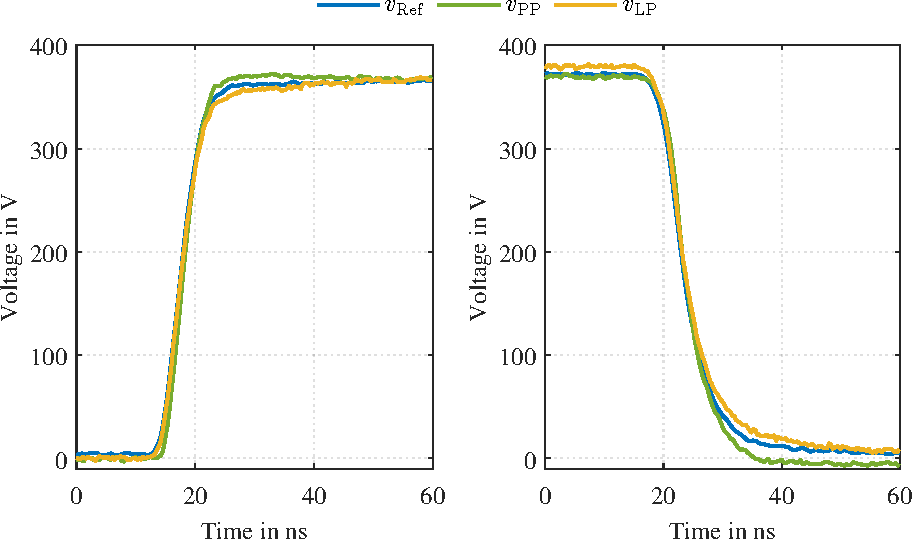
\includegraphics[scale=1]{figures/4_VoltageProbe/MS_PulsGen_TD.pdf}
	\caption{Large-signal verification time-domain of the low-pass using a \SI{50}{\ohm} pulse generator~\cite{kragl_active_2025}. The reference is acquired both via a conventional direct measurement and through a commercial \SI{180}{MHz}--\SI{340}{MHz} passive band-pass filter.}\label{fig:MS_PulsGen_TD}
\end{figure}

Datasheet for LP op states: 800MHz at 200mV, 250MHz at 2V and 140MHz at 4V. Plus BUF 3.1Ghz at 100mVpp, 1.6 at 2Vpp ...



\begin{figure}[ht]
	\centering
	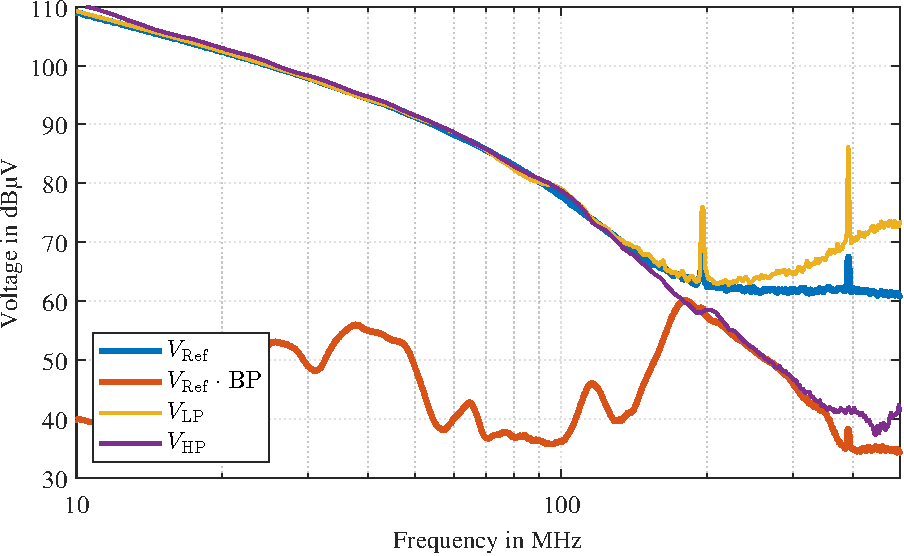
\includegraphics[scale=1]{figures/4_VoltageProbe/MS_PulsGen.pdf}
	\caption{Large-signal verification of the low-pass and high-pass channels using a \SI{50}{\ohm} pulse generator~\cite{kragl_active_2025}. The reference is acquired both via a conventional direct measurement and through a commercial \SI{180}{MHz}--\SI{340}{MHz} passive band-pass filter.}\label{fig:MS_PulsGen_Meas}
\end{figure}


% \begin{figure}[ht]
% 	\centering
% 	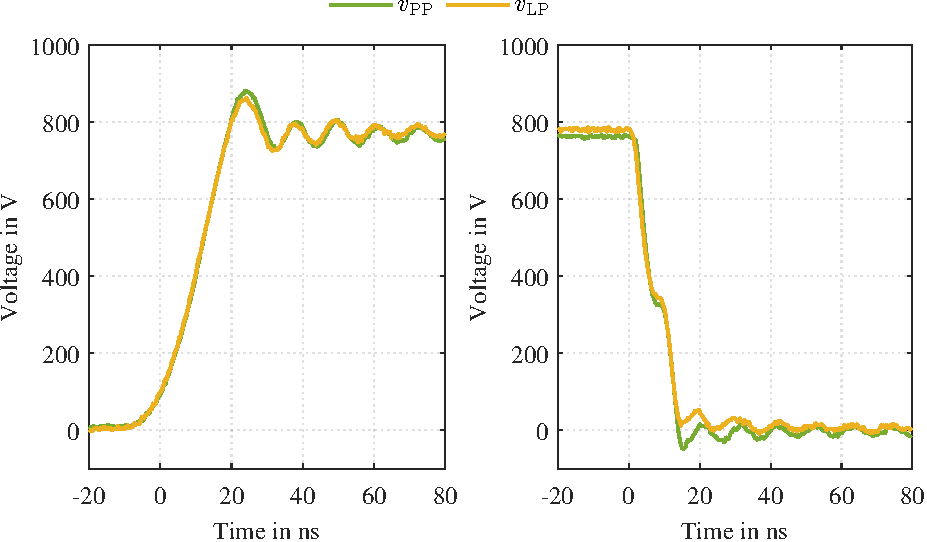
\includegraphics[scale=1]{figures/4_VoltageProbe/Voltage_DPT_EMEvsPP_TD.pdf}
% 	\caption{Time-domain measurement results of PMTX05, at 800V, 30A room temperature, cross validation of passive probe and low-pass measurement to crosscheck inductive and capacitive coupling effects.}\label{fig:Voltage_DPT_EMEvsPP_TD}
% \end{figure}


\subsection{Parasitic Couplings \& CM error}

\begin{figure}[ht]
	\centering
	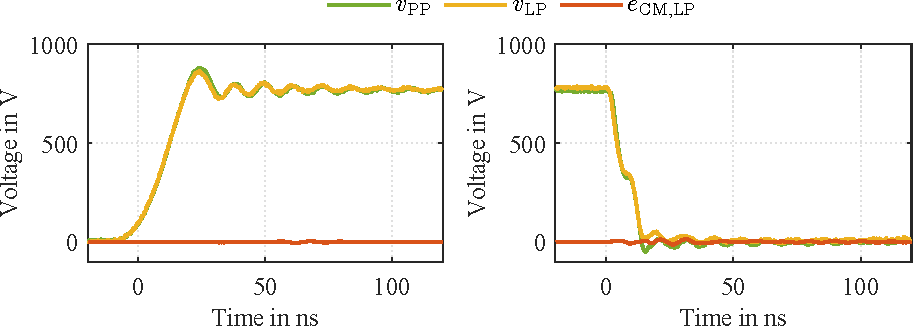
\includegraphics[scale=1]{figures/4_VoltageProbe/Voltage_DPT_LPvsPP_weCM_TD.pdf}
	\caption{Time-domain measurement results of PMTX05, at 800V, 30A room temperature, cross validation of passive probe and low-pass measurement to crosscheck inductive and capacitive coupling effects.}\label{fig:Voltage_DPT_LPvsPP_weCM_TD}
\end{figure}

\begin{figure}[ht]
	\centering
	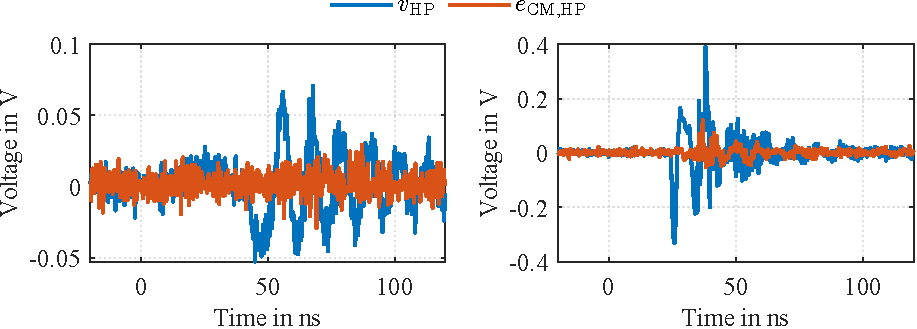
\includegraphics[scale=1]{figures/4_VoltageProbe/Voltage_DPT_HPvsPP_weCM_TD.pdf}
	\caption{Time-domain measurement results of PMTX05, at 800V, 30A room temperature, cross validation of passive probe and high-pass measurement to crosscheck inductive and capacitive coupling effects.}\label{fig:Voltage_DPT_HPvsPP_weCM_TD}
\end{figure}


The verification results demonstrate close agreement between the reference and the probe measurement for both the low-pass and high-pass channels in their respective frequency ranges.
The high-pass channel exhibits a maximum deviation of \SI{1.3}{dB} at \SI{200}{MHz}.
Above \SI{340}{MHz}, verification is no longer possible, as the commercial band-pass filter rolls off in this region.
No commercially available band-pass filter covers the \SIrange{300}{400}{MHz} frequency region, preventing independent verification in this range.

However, above \SI{340}{MHz}, the spectrum exhibits a plateau rather than the expected continuous decrease, indicating a measurement artifact that may increase the error beyond \SI{1.3}{dB} at higher frequencies.

Overall, the measurements demonstrate high repeatability, and the \SI{1.3}{dB} maximum deviation is considered sufficiently small for the intended analysis.
For the following analysis, the spectra are shown up to \SI{500}{MHz}, but the reader should be aware that the probe is only fully verified up to \SI{340}{MHz}.
Hence, results between \SI{340}{MHz} and \SI{500}{MHz} should be interpreted comparatively rather than as absolute calibrated values.







	%!TeX root = main.tex
%!encoding = UTF-8 Unicode


\chapter{Active Current Shunt}

While for lower frequencies mainly the capacitive coupling through the switched potential of the phase potential to the cooler dominate EMC concerns, at higher frequencies also inductive couplings occur.
Therefore it is necessary to measure not only the high-frequency components of the voltage transient but also of the current transient.


%!TeX root = main.tex
%!encoding = UTF-8 Unicode

\section{Requirements for Broadband, Low-Intrusion Current Sensing}

Prior to designing the active current shunt, the measurement-driven requirements are defined.
As in the voltage-probe chapter, the requirements are derived from the EMC-relevant frequency range, practical measurement constraints, and expected disturbance mechanisms in the switching environment.

\subsubsection*{Small Signal Response}
The current-sensing path must provide a bandwidth of at least \SI{500}{MHz} to cover the EMC-relevant spectral content of the commutation current.
This bandwidth requirement excludes commercial Rogowski coils for the present application, as their usable bandwidth is typically limited to approximately \SIrange{20}{50}{MHz}~\cite{xin_review_2022}.

\subsubsection*{Output Interface and Signal Routing}
Analogous to the voltage-probe concept, the current probe must provide a \SI{50}{\ohm} output interface.
This is required to route the measured signal into both low-pass and high-pass processing paths with defined impedance conditions.
Consequently, a purely passive shunt implementation is not sufficient for the intended measurement chain.

\subsubsection*{Isolation Requirement for Combined Measurements}
For standalone current measurements, galvanic isolation is not mandatory because the probe can reference the oscilloscope ground.
However, for simultaneous measurements with LISN disturbance voltage, galvanic isolation becomes necessary because the oscilloscope ground is fixed to the aluminum base plate.
In this case, optical isolation of the measurement link is feasible and compatible with the required \SI{50}{\ohm} signal interface.

\subsubsection*{Measurement Intrusion and Shunt Bandwidth}
The inserted sense resistance must be at least one decade below the on-state resistance \mi{R}{DS,on} of the DUT to avoid materially altering the transient damping behavior.
This is essential because the quality factor of the excited resonance is a key EMC-relevant characteristic.
For the considered \SI{750}{V} and \SI{1200}{V} discrete SiC devices in D2PAK, \mi{R}{DS,on} is in the range of \SIrange{20}{50}{m\ohm}~\cite{robert_bosch_gmbh_datasheet_2023,robert_bosch_gmbh_datasheet_2023-1}.
Accordingly, the sense resistance is limited to \SI{2}{m\ohm} or less.

This low resistance directly conflicts with the bandwidth target in conventional shunt realizations, because each shunt exhibits parasitic inductance.
The resulting shunt bandwidth is

\begin{equation}
    \mi{f}{bw,shunt} = \frac{1}{2\pi \tau_\text{shunt}} = \frac{\mi{R}{shunt}}{2\pi\mi{L}{shunt}} 
\end{equation}

In classical shunt design, larger shunt resistance values support higher bandwidth.
For the present EMC application, this trade-off cannot be exploited because the insertion resistance must remain very small.

\subsubsection*{Parasitic Coupling and Interconnect Length}
As for the voltage probe, parasitic coupling into the sensing path must be minimized, and the electrical interconnect length must be kept short enough to limit transmission-line effects.
For the active current shunt, parasitic coupling is particularly critical because the circuit is placed close to the switching node and operates with higher gain than the active voltage probe.


%!TeX root = main.tex
%!TeX root = main.tex
%!encoding = UTF-8 Unicode

\section{Active Current-Shunt Architecture and Implementation}

\begin{figure}[ht]
	\centering
	\tikzsetnextfilename{Diss_CompensatedCurrentShunt}
	\import{./figures/5_CurrentProbe/}{"Diss_CompensatedCurrentShunt.pdf_tex"}
	\caption{Simplified schematic overview of active current shunt.}\label{fig:ESBActiveShunt}
\end{figure}

\begin{figure}[ht]
	\centering
	\import{./figures/5_CurrentProbe/}{"Diss_Pic_AShunt.pdf_tex"}
	\caption{Photograph of active current shunt.}\label{fig:ESBActiveShuntPhoto}
\end{figure}

Therefore, a replica of the active shunt presented in~\cite{shillaber_gigahertz_2020,shillaber_ultrafast_2022} was designed. 
Its simplified equivalent circuit is shown in \fref{fig:ESBActiveShunt}, and a photograph of the prototype is shown in \fref{fig:ESBActiveShuntPhoto}.
This design offers multiple advantages:
First, a small shunt resistance can be used while still maintaining a sufficiently high sense output due to the amplification of the operational amplifier.
Furthermore, the low-pass filter of the active shunt compensates the high-pass characteristic of the shunt resistance, thereby achieving a remarkably high bandwidth.
Lastly, the compensation operational amplifier of the active shunt produces a defined output signal, which can either be fed into a filter stage for high-pass EM noise measurements or measured with an optically isolated voltage probe, thus providing galvanic isolation.



In contrast to~\cite{shillaber_gigahertz_2020,shillaber_ultrafast_2022}, extensive effort was required to sufficiently shield the sensitive active amplification from capacitive coupling from the switching-node potential, which would otherwise contaminate the measurement.
Best results were achieved with an ``EMC shield'' made of a nickel-silver alloy, which attenuates both capacitive and inductive coupling.
In addition to the shield, the transmission line between the passive shunt and the compensation amplifier was routed in the two inner PCB layers and enclosed by top and bottom ground planes connected by a via fence.



\subsection{Passive Shunt Element and Layout Realization}


\begin{figure}[ht]
	\centering
	\tikzsetnextfilename{Diss_PassiveShuntPCB_3D_wSchematic}
	\import{./figures/5_CurrentProbe/}{"Diss_PassiveShuntPCB_3D_wSchematic.pdf_tex"}
	\caption{Design of passive part of the current shunt.}\label{fig:ESBPassiveShunt}
\end{figure}






\subsection{Active Compensation for Bandwidth Extension and Impedance Matching}



\begin{figure}[ht]
	\centering
	\tikzsetnextfilename{Diss_Compensation_Shunt_ESB}
	\import{./figures/5_CurrentProbe/}{"Diss_Compensation_Shunt_ESB.pdf_tex"}
	\caption{Design of compensation part of the active current shunt.}\label{fig:ESBCompensation}
\end{figure}

\subsection{Amplification and Filter Path Design}

\subsubsection*{Low-Pass}

\begin{figure}[ht]
	\centering
	\tikzsetnextfilename{Diss_Lowpass_Shunt_ESB}
	\import{./figures/5_CurrentProbe/}{"Diss_Lowpass_Shunt_ESB.pdf_tex"}
	\caption{Design of low-pass part of the active current shunt.}\label{fig:ESBLowpass}
\end{figure}

\subsubsection*{High-Pass}

\begin{figure}[ht]
	\centering
	\tikzsetnextfilename{Diss_Highpass_Shunt_ESB}
	\import{./figures/5_CurrentProbe/}{"Diss_Highpass_Shunt_ESB.pdf_tex"}
	\caption{Design of high-pass part of the active current shunt.}\label{fig:ESBHighpass}
\end{figure}
%!TeX root = main.tex
%!encoding = UTF-8 Unicode


\section{Verification}

This section verifies the active current shunt in both the frequency and time domain.
Because the shunt is intended to resolve high-frequency commutation currents while preserving the low-frequency switching waveform, the verification must demonstrate not only the expected transfer behavior of the two filter paths, but also the overall usability of the probe in a measurement setup with finite source impedance and strong common-mode disturbance.

Accordingly, the verification is divided into a small-signal characterization using a vector network analyzer (VNA) and a large-signal validation using a passive shunt reference measurement.
The small-signal tests confirm the transfer functions of the low-pass and high-pass channels, while the large-signal tests assess the probe response under realistic switching conditions and verify that the active shunt does not introduce relevant distortion into the measured waveform.

\subsection{Small-Signal}

The VNA measurements of the low-pass and high-pass channels are shown in \fref{fig:VNA_Shunt_LP} and \fref{fig:VNA_Shunt_HP}.
For the low-pass path, the measured transfer includes the complete signal chain from the passive shunt through the compensation amplifier and low-pass filter to the VNA input.
The low-pass channel exhibits a bandwidth of \mi{f}{3dB} = \SI{475}{MHz} before the gain begins to rise.
Compared with the compensation-amplifier transfer function in \fref{fig:VNA_CompAmp}, this gain increase occurs at a higher frequency.
The reason is that the higher gain delays the point at which the secondary parasitic transmission path becomes dominant.
This bandwidth is more than sufficient for the intended SiC discrete-device measurements, where the noise floor typically starts to rise around \SI{100}{MHz}.
	
\begin{figure}[ht]
	\centering
	% This file was created by matlab2tikz.
%
%The latest updates can be retrieved from
%  http://www.mathworks.com/matlabcentral/fileexchange/22022-matlab2tikz-matlab2tikz
%where you can also make suggestions and rate matlab2tikz.
%
\definecolor{mycolor1}{rgb}{0.00000,0.44700,0.74100}%
\definecolor{mycolor2}{rgb}{0.85000,0.32500,0.09800}%
\definecolor{mycolor3}{rgb}{0.92900,0.69400,0.12500}%
\definecolor{mycolor4}{rgb}{0.49400,0.18400,0.55600}%
%
\begin{tikzpicture}

\begin{axis}[%
width=2.591in,
height=0.957in,
at={(0.616in,0.474in)},
scale only axis,
unbounded coords=jump,
xmode=log,
xmin=0.1,
xmax=1000,
xtick={0.1,1,10,100,1000},
xticklabels={{0.1},{1},{10},{100},{1000}},
xminorticks=true,
xlabel style={font=\color{white!15!black}},
xlabel={Frequency in MHz},
ymin=-120,
ymax=0,
ylabel style={font=\color{white!15!black}},
ylabel={Magnitude in dB},
axis background/.style={fill=white},
xmajorgrids,
xminorgrids,
ymajorgrids,
grid style={dotted},
legend style={at={(0.5,1.03)}, anchor=south, legend cell align=left, align=left, fill=none, draw=none},
legend columns = 4
]
\addplot [color=mycolor1, line width=1.5pt]
  table[row sep=crcr]{%
0.1	-0.01816616493\\
0.106349442	-0.01690826572\\
0.112698884	-0.01177073301\\
0.138482796	-0.009570624616\\
0.1725446	-0.01002667798\\
0.198281036	-0.01491078476\\
0.219753858	-0.01122766743\\
0.291109957	-0.01453728435\\
0.344627992	-0.0144176859\\
0.446255517	-0.01466776159\\
0.497605565	-0.01379297952\\
0.546753616	-0.01510196244\\
1.632240533	-0.01508187313\\
11.99531021	-0.02139159331\\
18.85543879	-0.02558769899\\
32.03721498	-0.03286254809\\
39.73397101	-0.03657987226\\
53.70000506	-0.04281928757\\
131.4730623	-0.06950909163\\
282.7730138	-0.1017708403\\
329.0158078	-0.1111759172\\
344.0396394	-0.09936534832\\
350.4784243	-0.1029096142\\
359.0634709	-0.09087256654\\
371.9410408	-0.1019650848\\
380.5260874	-0.09073750277\\
401.988704	-0.1054924715\\
417.0125355	-0.1042022018\\
428.4054685	-0.1084264984\\
431.3651992	-0.1033617309\\
434.32493	-0.1100306159\\
440.2443915	-0.101593645\\
446.163853	-0.1114931586\\
458.0027759	-0.112084918\\
469.8416989	-0.1111202812\\
481.6806219	-0.1132454342\\
487.6000834	-0.1234797659\\
499.4390064	-0.1098537975\\
502.3987372	0.07314965416\\
nan	nan\\
511.2779294	0.007344708969\\
514.2376601	-0.1122263874\\
517.1973909	-0.08214171247\\
520.1571216	0.1105124474\\
nan	nan\\
529.0363139	0.02889304633\\
537.9155061	-0.1208650818\\
573.4322751	-0.1137035457\\
576.8889099	0.2672458068\\
nan	nan\\
589.0986518	0.03818298189\\
601.3083936	-0.1211315156\\
613.5181355	-0.1290170649\\
646.0774471	-0.1243407895\\
654.217275	-0.1171832491\\
658.2871889	0.3247927109\\
nan	nan\\
690.8465005	0.2813638476\\
703.0562424	-0.129694273\\
711.1960703	-0.06261471623\\
715.2659843	-0.1322730956\\
739.685468	-0.1510730607\\
764.1049517	-0.1448210481\\
788.5244354	-0.149208805\\
826.9631436	-0.1606742902\\
894.3341504	-0.1472239124\\
944.8624056	-0.1612820546\\
989.7764101	-0.1487663639\\
1001.004911	-0.1477712303\\
};
\addlegendentry{$\mathrm{S}_\mathrm{11}$}

\addplot [color=mycolor2, line width=1.5pt]
  table[row sep=crcr]{%
0.1	-90.56814014\\
0.100705494	-96.88295613\\
0.101410987	-89.07895684\\
0.102116481	-92.1975316\\
0.102821974	-91.81817866\\
0.103527468	-108.7492756\\
0.104232961	-93.74855862\\
0.104938455	-96.52511842\\
0.105643948	-96.30135231\\
0.107054935	-90.43724334\\
0.107760429	-95.91269435\\
0.108465922	-90.67295735\\
0.109876909	-100.0705598\\
0.110582403	-88.55027834\\
0.112698884	-96.1189421\\
0.113404377	-91.74383941\\
0.114109871	-99.49870695\\
0.115520858	-87.79120717\\
0.116226351	-90.50936768\\
0.116931845	-88.3328983\\
0.117637338	-98.36369265\\
0.119048325	-91.31574339\\
0.119753819	-92.17853912\\
0.120459312	-88.92292899\\
0.121164806	-91.81123625\\
0.1218703	-102.4405326\\
0.12398678	-89.55752108\\
0.124692274	-94.36806555\\
0.125397767	-93.0604946\\
0.126103261	-99.03173997\\
0.126808754	-96.94754445\\
0.127514248	-88.28775528\\
0.128925235	-90.01807606\\
0.129630728	-101.799078\\
0.131041715	-91.73995317\\
0.131747209	-102.6379645\\
0.132452703	-88.92096064\\
0.133158196	-105.7292538\\
0.134569183	-93.69902266\\
0.135274677	-96.43961683\\
0.13598017	-89.03906886\\
0.136685664	-91.32038958\\
0.137509601	-90.75663574\\
0.13945599	-97.29351284\\
0.140429185	-88.68162591\\
0.141402379	-98.50200252\\
0.142375573	-94.49769312\\
0.144321962	-99.40118738\\
0.146268351	-90.89506769\\
0.147241545	-93.52950038\\
0.14821474	-109.2142064\\
0.149187934	-99.44652422\\
0.151134323	-107.4688956\\
0.152107517	-91.10842569\\
0.153080712	-93.76825211\\
0.154053906	-106.5895076\\
0.155027101	-94.25361451\\
0.156000295	-97.44637535\\
0.156973489	-90.91016526\\
0.157946684	-102.1954493\\
0.159893073	-96.96360246\\
0.160866267	-103.9437463\\
0.162812656	-94.91851954\\
0.164759045	-97.64917746\\
0.165732239	-103.6003035\\
0.168651822	-96.19457427\\
0.170598211	-98.04391858\\
0.171571405	-94.04637387\\
0.1725446	-100.9946312\\
0.174490989	-94.87234767\\
0.175464183	-109.5653393\\
0.176437377	-92.17250439\\
0.177410572	-101.8272965\\
0.178383766	-93.17557544\\
0.179356961	-105.128516\\
0.181303349	-91.08722571\\
0.183249738	-97.19080822\\
0.184222933	-96.07220291\\
0.186169321	-103.5422885\\
0.187142516	-97.72503852\\
0.18811571	-101.7483645\\
0.189088905	-90.62783753\\
0.190228728	-98.11155619\\
0.194254882	-90.87532806\\
0.195596933	-119.2363945\\
0.198281036	-98.11458012\\
0.199623087	-98.28011993\\
0.200965139	-97.27804111\\
0.20230719	-106.7054686\\
0.204991293	-97.3539136\\
0.206333344	-99.56957007\\
0.207675395	-92.38492743\\
0.213043601	-100.9380642\\
0.214385652	-100.6018674\\
0.215727704	-90.53388552\\
0.217069755	-96.61927159\\
0.218411806	-94.3173419\\
0.22243796	-102.5012777\\
0.225122063	-95.41696508\\
0.226464115	-102.7431429\\
0.227806166	-94.73613904\\
0.230490269	-104.4733699\\
0.23183232	-93.67556649\\
0.235858474	-102.4307894\\
0.238542577	-96.00652682\\
0.239884628	-103.9823073\\
0.24122668	-97.75074053\\
0.242568731	-106.4061834\\
0.245252834	-94.53319844\\
0.246594885	-125.9872536\\
0.247936937	-95.11894462\\
0.249278988	-107.1224183\\
0.251963091	-93.58772367\\
0.253305142	-93.83153168\\
0.254647193	-95.45837927\\
0.258673347	-107.3126867\\
0.260015399	-97.76960141\\
0.261582765	-101.8154612\\
0.263428214	-93.45047028\\
0.267119113	-103.5028065\\
0.270810012	-95.43297372\\
0.272655462	-102.887244\\
0.274500911	-96.35553487\\
0.276346361	-98.80387366\\
0.28003726	-93.99952971\\
0.281882709	-95.88844321\\
0.283728159	-93.59180995\\
0.285573608	-100.4580955\\
0.287419058	-96.17143861\\
0.289264507	-107.0144256\\
0.292955406	-101.0675425\\
0.294800856	-107.9337457\\
0.296646305	-100.1066814\\
0.298491755	-101.641747\\
0.300337204	-98.74623031\\
0.302182654	-104.8543312\\
0.304028103	-99.05339456\\
0.307719002	-109.7219324\\
0.309564452	-121.7804001\\
0.313255351	-96.67479573\\
0.3151008	-102.7394325\\
0.31694625	-130.1769687\\
0.320637149	-97.64177041\\
0.328018947	-118.5072505\\
0.331709845	-94.6478901\\
0.333555295	-106.0616617\\
0.339091643	-92.40581835\\
0.342782542	-104.967175\\
0.35016434	-96.94048684\\
0.355700689	-108.3856725\\
0.357546138	-92.98296302\\
0.359701417	-100.0942542\\
0.362247126	-98.7064259\\
0.364792835	-99.48620559\\
0.367338544	-106.2055218\\
0.369884252	-99.3023719\\
0.372429961	-101.7783577\\
0.37497567	-99.17569079\\
0.377521379	-104.2411042\\
0.380067088	-99.87871133\\
0.385158505	-104.296773\\
0.387704214	-111.9151803\\
0.392795632	-100.4552064\\
0.395341341	-101.1546618\\
0.402978467	-94.02670996\\
0.405524176	-104.6603056\\
0.408069885	-103.3247741\\
0.410615594	-121.3016594\\
0.413161302	-103.8561422\\
0.415707011	-109.4272418\\
0.41825272	-98.57397695\\
0.423344138	-106.0133229\\
0.428435555	-99.89984324\\
0.430981264	-103.3912689\\
0.433526973	-98.01088196\\
0.436072682	-116.1236918\\
0.441164099	-94.3200908\\
0.443709808	-99.29965529\\
0.446255517	-96.78110731\\
0.451346935	-105.5900237\\
0.453892644	-103.9076726\\
0.458984061	-94.22124142\\
0.466621188	-107.7582742\\
0.471712605	-99.86733052\\
0.474258314	-102.9409465\\
0.479349732	-99.31917373\\
0.484441149	-100.9278441\\
0.486986858	-98.94312937\\
0.489532567	-99.14041244\\
0.492078276	-98.72005423\\
0.494623985	-95.99858932\\
0.497605565	-104.4427675\\
0.50111614	-99.44640328\\
0.504626715	-103.0030652\\
0.50813729	-95.27773646\\
0.511647866	-104.4690589\\
0.515158441	-95.85374201\\
0.522179591	-107.9350318\\
0.525690166	-97.60990704\\
0.529200741	-102.8353866\\
0.532711316	-96.23928503\\
0.539732466	-114.6393015\\
0.546753616	-98.56870904\\
0.550264191	-102.4631852\\
0.560795917	-98.37952697\\
0.567817067	-107.8490521\\
0.574838217	-103.0100341\\
0.581859367	-106.8714284\\
0.585369942	-95.37261074\\
0.588880517	-97.66101408\\
0.592391092	-97.31925449\\
0.599412243	-118.1356477\\
0.606433393	-92.95429957\\
0.616965118	-108.9167858\\
0.620475693	-98.22781809\\
0.623986268	-104.8861125\\
0.627496843	-102.850243\\
0.631007418	-96.06846619\\
0.634517993	-101.6985767\\
0.638028568	-101.2768765\\
0.641539144	-96.46365963\\
0.652070869	-108.5159635\\
0.659092019	-95.17700201\\
0.662602594	-107.0348496\\
0.673134319	-97.00897964\\
0.680155469	-101.5161732\\
0.684255429	-100.0817493\\
0.693940768	-109.7600515\\
0.698783437	-96.90484079\\
0.703626107	-101.0172012\\
0.708468776	-99.37002939\\
0.713311446	-102.9295627\\
0.718154115	-101.0065509\\
0.722996785	-107.5726127\\
0.732682124	-94.84210524\\
0.742367463	-100.6176711\\
0.747210132	-98.71763792\\
0.756895471	-106.662915\\
0.76658081	-100.7898886\\
0.77142348	-119.410664\\
0.776266149	-102.0277923\\
0.781108819	-107.105402\\
0.785951488	-99.72058834\\
0.790794158	-116.6009072\\
0.795636827	-99.35835234\\
0.805322166	-110.6359316\\
0.810164836	-97.10149137\\
0.815007505	-101.5595078\\
0.824692844	-99.13791508\\
0.829535514	-111.9498816\\
0.839220853	-94.67555332\\
0.844063522	-100.5435047\\
0.848906192	-100.5015727\\
0.853748861	-104.9827186\\
0.858591531	-102.1070009\\
0.8634342	-115.2590776\\
0.877962209	-99.7546645\\
0.882804878	-103.7571193\\
0.902175556	-99.03516778\\
0.907018226	-103.0042834\\
0.911860895	-96.06807582\\
0.916703565	-105.2348117\\
0.921546234	-97.3711783\\
0.926388904	-104.7945842\\
0.931231573	-104.0443067\\
0.936074243	-99.04006054\\
0.940916912	-113.5838051\\
0.953266857	-99.96938314\\
0.973301224	-107.9651885\\
0.979979347	-98.90421329\\
1.000013714	-111.0078168\\
1.013369958	-95.24530653\\
1.02004808	-102.1843343\\
1.026726203	-95.46046445\\
1.033404325	-101.3400746\\
1.040082447	-97.34320806\\
1.04676057	-102.1668012\\
1.060116814	-99.00266486\\
1.066794937	-99.70182082\\
1.073473059	-103.6518439\\
1.080151181	-96.67064195\\
1.086829304	-104.2649786\\
1.093507426	-101.2920884\\
1.100185548	-104.3573016\\
1.120219915	-101.3997585\\
1.126898037	-105.4682464\\
1.13357616	-96.80893129\\
1.140254282	-117.7892034\\
1.146932404	-96.75616418\\
1.153610527	-104.9796716\\
1.160288649	-99.03046897\\
1.173644894	-111.0239729\\
1.180323016	-100.834764\\
1.187001138	-104.0158785\\
1.19367926	-102.5107078\\
1.200357383	-96.37118614\\
1.213713627	-101.9271092\\
1.22039175	-98.19952102\\
1.227069872	-107.0444695\\
1.233747994	-100.261753\\
1.253782361	-111.1088514\\
1.267138606	-95.28673389\\
1.273816728	-96.7944818\\
1.28049485	-95.66706904\\
1.287172973	-105.3399827\\
1.293851095	-104.581597\\
1.301650396	-97.89288158\\
1.310833455	-106.1220519\\
1.320016515	-98.87270661\\
1.338382633	-104.7792776\\
1.347565693	-100.0308235\\
1.356748752	-102.3455292\\
1.365931811	-98.01152873\\
1.375114871	-98.12120797\\
1.38429793	-99.63047565\\
1.393480989	-107.0879598\\
1.411847108	-96.07594913\\
1.421030167	-98.11301999\\
1.430213227	-95.12464247\\
1.448579346	-103.8809408\\
1.457762405	-100.9596231\\
1.466945464	-101.3239998\\
1.476128524	-104.2875282\\
1.485311583	-96.40166838\\
1.494494642	-97.4146711\\
1.512860761	-109.7909069\\
1.52204382	-129.988048\\
1.53122688	-98.99125741\\
1.549592999	-106.5986054\\
1.558776058	-98.09860042\\
1.567959117	-102.6698187\\
1.577142177	-101.6461807\\
1.586325236	-101.8775435\\
1.595508295	-107.4096705\\
1.613874414	-99.58112694\\
1.641423592	-105.9951884\\
1.650606652	-97.04304203\\
1.659789711	-102.0718586\\
1.66897277	-101.0371944\\
1.687338889	-103.5170687\\
1.696521948	-100.1605037\\
1.705705008	-103.1609537\\
1.714888067	-96.47240996\\
1.733254186	-110.9287005\\
1.751620305	-98.23429005\\
1.760803364	-108.6507617\\
1.769986423	-95.47511692\\
1.779169483	-96.14068671\\
1.78989427	-102.0280033\\
1.802561859	-96.82376844\\
1.815229447	-106.3928257\\
1.827897036	-103.8091524\\
1.840564625	-103.8750251\\
1.865899803	-110.6437926\\
1.878567391	-97.86157248\\
1.916570158	-102.6862545\\
1.929237746	-100.8086192\\
1.941905335	-116.1838968\\
1.954572924	-96.45921063\\
2.005243279	-120.3605316\\
2.017910868	-100.5966846\\
2.030578457	-105.0429688\\
2.055913634	-102.1834404\\
2.081248812	-109.234148\\
2.0939164	-98.48557316\\
2.144586756	-103.280029\\
2.169921933	-99.41589143\\
2.182589522	-112.543903\\
2.207924699	-97.68361921\\
2.220592288	-108.02314\\
2.233259877	-98.16026105\\
2.245927466	-99.09950795\\
2.271262643	-96.43093057\\
2.30926541	-106.0274676\\
2.321932998	-92.52325491\\
2.334600587	-103.9445953\\
2.347268176	-99.23588569\\
2.359935765	-108.2546251\\
2.372603353	-97.61838567\\
2.397938531	-106.2536618\\
2.423273708	-100.7978159\\
2.435941297	-102.4964457\\
2.461276475	-94.48744063\\
2.476112985	-97.23917909\\
2.493581802	-116.1855415\\
2.511050619	-97.9981374\\
2.545988253	-106.4041754\\
2.598394704	-102.5259646\\
2.615863521	-104.2300445\\
2.633332338	-97.44267949\\
2.668269972	-108.5900921\\
2.685738789	-104.1118537\\
2.703207606	-105.826885\\
2.720676423	-103.4786719\\
2.73814524	-104.5963689\\
2.755614057	-104.3526892\\
2.790551691	-99.04251809\\
2.825489325	-106.9919229\\
2.860426959	-102.845944\\
2.877895776	-96.35135316\\
2.91283341	-108.5570425\\
2.930302227	-107.9271813\\
2.965239861	-95.86047381\\
3.017646312	-104.7479304\\
3.035115129	-98.17483899\\
3.087521579	-113.4208627\\
3.122459213	-103.3506184\\
3.13992803	-107.93347\\
3.157396847	-97.83066932\\
3.174865664	-110.5656193\\
3.192334481	-108.4109307\\
3.209803298	-112.3637158\\
3.227272115	-103.6661485\\
3.244740932	-106.8191796\\
3.262209749	-99.21771398\\
3.279678566	-99.40733086\\
3.297147383	-105.6905533\\
3.3146162	-97.55476746\\
3.332085017	-102.8352344\\
3.349553834	-100.0255232\\
3.367022651	-105.2374507\\
3.384491468	-105.0447384\\
3.404893095	-100.4521677\\
3.428914395	-108.408841\\
3.476956996	-97.10126839\\
3.500978297	-100.1245677\\
3.524999597	-116.2252111\\
3.549020898	-92.97552383\\
3.597063499	-114.4102031\\
3.6210848	-104.001956\\
3.6451061	-104.3720709\\
3.669127401	-98.96379137\\
3.693148702	-103.6858664\\
3.717170002	-98.97514439\\
3.741191303	-101.2375431\\
3.765212603	-113.3585423\\
3.789233904	-102.944717\\
3.813255204	-116.9128489\\
3.837276505	-114.4895321\\
3.861297806	-102.2637635\\
3.885319106	-109.8836921\\
3.909340407	-100.7184014\\
3.933361707	-103.5154335\\
3.957383008	-99.29868857\\
3.981404309	-110.0047071\\
4.005425609	-108.7532157\\
4.02944691	-97.99820435\\
4.05346821	-102.9173045\\
4.077489511	-102.7858575\\
4.101510811	-100.6932613\\
4.125532112	-104.4271594\\
4.173574713	-99.22592949\\
4.197596014	-101.3655614\\
4.269659915	-99.13022669\\
4.293681216	-104.5964514\\
4.365745118	-97.19761462\\
4.389766418	-107.7470692\\
4.413787719	-107.3441486\\
4.43780902	-100.6927011\\
4.485851621	-107.8051678\\
4.509872921	-96.42095416\\
4.533894222	-104.9092002\\
4.557915522	-102.1928865\\
4.581936823	-107.8077933\\
4.629979424	-103.3199803\\
4.654000725	-105.7591983\\
4.68205492	-93.84584795\\
4.748327378	-103.3663417\\
4.781463607	-98.07907732\\
4.814599836	-102.9918901\\
4.847736065	-100.4630988\\
4.880872294	-103.7754171\\
4.914008523	-99.72001304\\
4.947144752	-100.7502665\\
4.980280981	-107.4135139\\
5.01341721	-100.8972592\\
5.046553439	-108.254108\\
5.112825896	-95.40622584\\
5.145962125	-121.4938877\\
5.212234583	-101.2575159\\
5.245370812	-102.7331586\\
5.278507041	-98.44446745\\
5.31164327	-116.2424764\\
5.377915728	-107.1312177\\
5.411051957	-110.4873193\\
5.477324415	-94.46056424\\
5.543596873	-102.2200751\\
5.576733102	-95.46642933\\
5.609869331	-101.989194\\
5.64300556	-94.53572817\\
5.676141789	-105.9321463\\
5.742414247	-99.13031851\\
5.841822933	-106.2777\\
5.974367849	-97.3462899\\
6.007504078	-105.2532015\\
6.040640307	-102.9905792\\
6.073776536	-103.3600028\\
6.106912765	-111.3268007\\
6.140048994	-99.95611857\\
6.173185223	-112.4366744\\
6.239457681	-96.1673531\\
6.27259391	-118.3769683\\
6.338866368	-99.31099205\\
6.372002597	-116.1203822\\
6.438275055	-97.31541267\\
6.477084809	-111.8483265\\
6.614171052	-103.0425699\\
6.659866467	-109.3247705\\
6.751257296	-102.0557652\\
6.842648125	-108.4950819\\
6.934038953	-98.63616271\\
7.025429782	-103.7056372\\
7.071125197	-100.2534472\\
7.116820611	-105.3857897\\
7.162516026	-102.2349102\\
7.299602269	-119.4288202\\
7.345297683	-105.1064121\\
7.436688512	-116.5781767\\
7.482383927	-113.6842071\\
7.528079341	-97.55592385\\
7.573774756	-104.5532669\\
7.61947017	-104.5068858\\
7.665165585	-105.9748054\\
7.710860999	-103.2704047\\
7.756556413	-106.6973808\\
7.802251828	-106.1996295\\
7.847947242	-101.5514406\\
7.893642657	-107.6135208\\
7.939338071	-105.7676101\\
7.985033486	-119.936883\\
8.076424314	-100.2060775\\
8.122119729	-104.5983132\\
8.167815143	-102.2158551\\
8.259205972	-109.353251\\
8.304901387	-104.2507969\\
8.350596801	-105.1630275\\
8.487683044	-96.14441715\\
8.533378459	-97.33585096\\
8.624769288	-108.9547116\\
8.670464702	-100.4514836\\
8.716160117	-106.525955\\
8.761855531	-106.0838523\\
8.807550946	-99.26815508\\
8.85324636	-110.1133065\\
8.906613499	-101.1617967\\
8.969648125	-104.182019\\
9.095717379	-99.85854277\\
9.158752005	-100.7381466\\
9.221786632	-103.6087497\\
9.284821259	-103.0353068\\
9.347855886	-98.7752776\\
9.410890512	-101.9567698\\
9.473925139	-113.3920963\\
9.599994392	-97.57948363\\
9.663029019	-98.00529745\\
9.726063646	-104.4051768\\
9.852132899	-103.3778471\\
9.915167526	-107.3160642\\
9.978202153	-98.15785171\\
10.16730603	-112.9029334\\
10.23034066	-100.5009127\\
10.29337529	-104.5711793\\
10.35640991	-104.1774224\\
10.41944454	-99.66630027\\
10.54551379	-110.489602\\
10.60854842	-95.7810518\\
10.67158305	-104.6778239\\
10.73461767	-96.77145269\\
10.86068693	-99.736514\\
10.92372155	-96.21557573\\
11.11282543	-105.074408\\
11.17586006	-100.4196802\\
11.23889469	-125.2216212\\
11.36496394	-103.0524117\\
11.42799857	-103.5427282\\
11.49103319	-103.1695215\\
11.61710245	-106.7073558\\
11.68013707	-111.1018577\\
11.80620633	-102.0395549\\
11.93227558	-106.0911415\\
12.05834483	-100.0303471\\
12.18441409	-113.5098908\\
12.24744871	-100.3148016\\
12.49512763	-116.4808008\\
12.66897924	-101.1137114\\
12.84283085	-111.6149175\\
13.10360827	-99.86924587\\
13.19053407	-112.0975335\\
13.27745988	-100.9085908\\
13.36438568	-101.4359221\\
13.6251631	-106.2209525\\
13.7120889	-103.1009196\\
13.79901471	-105.4447674\\
14.05979212	-101.6185695\\
14.14671793	-106.2544132\\
14.23364374	-96.82177346\\
14.40749535	-104.8320763\\
14.49442115	-98.65915608\\
14.58134696	-102.4944188\\
14.66827276	-96.33870635\\
14.75519857	-113.1100077\\
14.84212437	-97.94839819\\
14.92905018	-108.8364294\\
15.10290179	-98.27899059\\
15.1898276	-104.7074143\\
15.36367921	-103.7118686\\
15.45060501	-96.38770883\\
15.53753082	-101.7002791\\
15.62445662	-121.0336886\\
15.88523404	-101.8332245\\
15.97215985	-103.4543562\\
16.05908565	-111.7238246\\
16.14601146	-101.4823636\\
16.31986307	-106.9503541\\
16.40678887	-105.5667195\\
16.58064048	-93.5258053\\
16.75449209	-108.0177462\\
16.8414179	-101.0582462\\
17.06246886	-107.2901129\\
17.18200019	-100.7121799\\
17.30153151	-109.4370703\\
17.42106284	-104.0052187\\
17.54059417	-111.137184\\
17.77965683	-97.13903254\\
17.89918816	-120.9399907\\
18.01871949	-94.79752829\\
18.13825081	-95.81209807\\
18.25778214	-104.3442636\\
18.37731347	-99.79912512\\
18.61637613	-120.699647\\
18.85543878	-98.36422122\\
18.97497011	-108.4987018\\
19.09450144	-107.293994\\
19.21403277	-112.1300778\\
19.3335641	-97.6670215\\
19.45309543	-116.3903024\\
19.81168941	-98.79942783\\
19.93122074	-100.2584571\\
20.05075207	-100.0089234\\
20.1702834	-97.60676933\\
20.40934606	-100.1599165\\
20.52887738	-104.5147586\\
20.64840871	-99.05243801\\
20.76794004	-100.5289032\\
20.88747137	-106.8454623\\
21.0070027	-106.1913867\\
21.12653403	-100.5683275\\
21.36559668	-104.2543398\\
21.48512801	-103.9491682\\
21.60465934	-106.5157829\\
21.72419067	-100.8816329\\
21.96325333	-105.8045933\\
22.08278466	-98.64333785\\
22.32184731	-114.5968047\\
22.44137864	-100.2561866\\
22.56090997	-108.395908\\
22.6804413	-102.0047276\\
22.79997263	-112.6605871\\
23.15856661	-101.4806098\\
23.29816585	-106.9131687\\
23.46305357	-101.4656807\\
23.62794129	-105.7237143\\
24.12260445	-100.5359951\\
24.6172676	-112.3170312\\
24.78215532	-105.6762972\\
24.94704304	-109.1926634\\
25.11193076	-103.9351172\\
25.27681848	-108.6072582\\
25.77148164	-97.4862448\\
26.2661448	-117.0702488\\
26.43103252	-99.1015304\\
26.59592024	-103.9927546\\
27.09058339	-96.09252468\\
27.25547111	-100.9809284\\
27.42035883	-97.90188548\\
27.75013427	-106.4420731\\
27.91502199	-102.9540502\\
28.07990971	-105.5203767\\
28.24479743	-103.8278137\\
28.40968515	-117.3381457\\
28.73946059	-98.04087771\\
29.23412375	-115.7610587\\
29.56389918	-97.170193\\
29.7287869	-101.7120663\\
29.89367462	-101.0074288\\
30.05856234	-116.4299144\\
30.22345006	-99.38171413\\
30.5532255	-112.0385261\\
31.04788866	-103.1181861\\
31.21277638	-111.5598036\\
31.54255182	-94.91355164\\
31.87232726	-113.0707946\\
32.03721498	-98.4279178\\
32.23033447	-98.81393592\\
32.91248325	-117.9904267\\
33.3672491	-102.5712762\\
33.59463202	-112.6228468\\
34.04939788	-100.5469754\\
34.2767808	-103.5471706\\
34.50416373	-114.876164\\
34.73154665	-99.01798415\\
35.1863125	-100.8045028\\
35.41369543	-96.42482891\\
35.64107835	-100.4431081\\
35.86846128	-99.60468551\\
36.0958442	-102.7683149\\
36.32322713	-99.23169353\\
36.55061005	-100.2671229\\
36.77799298	-106.1139925\\
37.00537591	-101.9562073\\
37.23275883	-107.5501145\\
37.68752468	-98.23289361\\
37.91490761	-105.1329774\\
38.36967346	-101.0452321\\
38.59705638	-113.6813455\\
39.05182223	-97.93058213\\
39.27920516	-104.7694771\\
39.50658808	-102.3449822\\
39.73397101	-103.8087131\\
39.96135393	-113.151412\\
40.41611978	-96.41016523\\
41.32565149	-107.0714129\\
41.55303441	-95.90860683\\
41.78041734	-108.3265548\\
42.00780026	-99.52465233\\
42.68994904	-106.2166856\\
42.91733196	-97.06829364\\
43.37209781	-110.3458015\\
43.59948074	-96.72012891\\
44.05424659	-113.2840266\\
44.6324778	-96.42823365\\
44.94515115	-98.1831171\\
45.2578245	-107.866068\\
45.57049786	-103.2016945\\
45.88317121	-104.8364973\\
46.19584457	-110.9854583\\
46.50851792	-102.6210135\\
46.82119127	-105.2465961\\
47.44653798	-101.1457361\\
47.75921134	-115.7203619\\
48.07188469	-98.42635073\\
48.6972314	-104.7063795\\
49.00990475	-103.3876973\\
49.32257811	-119.0700147\\
49.94792482	-99.94388143\\
50.26059817	-107.4359901\\
50.57327152	-100.7593741\\
50.88594488	-108.83765\\
51.19861823	-108.2803946\\
51.51129158	-106.379699\\
52.13663829	-97.82343616\\
52.44931165	-117.1537882\\
52.761985	-103.1182298\\
53.07465836	-107.8529314\\
53.38733171	-97.04088072\\
53.70000506	-116.2125673\\
54.63802513	-98.58131858\\
55.57604519	-112.3497267\\
55.88871854	-100.1773018\\
56.2013919	-109.0256758\\
56.51406525	-99.13395697\\
56.82673861	-113.2162589\\
57.13941196	-97.62471135\\
57.45208531	-104.8246711\\
57.76475867	-97.6858269\\
58.07743202	-103.2748771\\
58.39010537	-100.2689931\\
58.70277873	-101.8249307\\
59.01545208	-97.23761276\\
59.32812544	-98.88580104\\
59.64079879	-107.8907618\\
59.95347215	-107.7572301\\
60.2661455	-108.9370886\\
60.57881885	-125.4892862\\
61.37530425	-103.8916138\\
62.66925782	-115.5125698\\
63.10057567	-101.9712988\\
63.53189353	-104.3029203\\
63.96321139	-111.0902419\\
64.39452924	-98.48771147\\
64.82584709	-110.7365381\\
65.25716495	-109.5446954\\
65.68848281	-120.7459559\\
66.11980066	-99.36713621\\
66.55111852	-114.2536443\\
67.41375423	-99.03663301\\
68.27638994	-107.8803463\\
69.13902565	-99.827425\\
69.5703435	-117.0685884\\
70.00166136	-100.4531427\\
70.43297921	-100.7972343\\
70.86429707	-110.0437879\\
71.29561493	-99.48004579\\
72.15825064	-107.9988958\\
73.02088635	-104.226548\\
73.88352206	-108.9135868\\
74.31483991	-107.0828876\\
74.74615777	-99.75726961\\
75.17747562	-105.1868803\\
75.60879348	-97.66538559\\
76.47142919	-107.2045872\\
77.76538276	-99.78460541\\
78.19670061	-102.5264494\\
79.05933632	-97.8071234\\
79.49065418	-105.8476678\\
80.35328989	-97.40448818\\
80.78460774	-114.0981803\\
81.2159256	-97.21674313\\
81.64724345	-107.2928717\\
82.07856131	-107.1709299\\
83.37251487	-95.23015213\\
83.80383273	-114.6715825\\
84.30900005	-104.9330234\\
84.90379459	-107.561065\\
85.49858914	-101.7788235\\
86.68817822	-123.2716988\\
87.28297277	-102.4064066\\
87.87776731	-130.2849667\\
89.0673564	-95.2039152\\
89.66215094	-96.89446858\\
90.85174002	-115.9332063\\
91.44653457	-98.01852545\\
92.04132911	-120.0881441\\
92.63612365	-99.7725944\\
93.82571274	-108.3502423\\
95.01530183	-102.2537023\\
95.61009637	-106.986598\\
96.79968545	-104.1947785\\
97.39448	-112.74367\\
98.58406908	-96.87266578\\
99.17886362	-97.22348199\\
99.77365817	-99.39153994\\
100.3684527	-96.6421027\\
102.1528363	-107.422451\\
103.93722	-98.03660477\\
104.5320145	-110.1224541\\
105.7216036	-105.3474439\\
106.3163981	-109.4490439\\
106.9111927	-100.3229767\\
107.5059872	-102.513235\\
108.6955763	-97.98508769\\
109.2903709	-107.6773084\\
109.8851654	-106.5758713\\
110.4799599	-100.0853485\\
111.0747545	-107.2792104\\
112.2643436	-100.3627593\\
112.8591381	-103.2603992\\
114.0487272	-94.95202338\\
114.6435217	-105.0511289\\
115.2383163	-97.16190314\\
115.9329699	-118.7208866\\
116.7508695	-98.4956059\\
117.5687691	-108.2707947\\
118.3866687	-100.1278411\\
119.2045683	-100.8817383\\
120.0224679	-109.1884368\\
120.8403675	-99.2868633\\
121.6582671	-101.9393083\\
122.4761667	-98.57525865\\
123.2940663	-103.1544782\\
124.1119659	-101.4221106\\
124.9298655	-105.6781873\\
125.7477651	-99.55648101\\
127.3835643	-104.2518237\\
128.2014639	-98.1834526\\
129.8372631	-108.2501037\\
130.6551627	-99.06075285\\
131.4730623	-100.7347939\\
132.2909619	-100.1925151\\
133.1088616	-101.45384\\
133.9267612	-96.20866913\\
134.7446608	-114.4015587\\
137.1983596	-100.9545198\\
138.0162592	-115.9156393\\
138.8341588	-102.364311\\
139.6520584	-109.3102057\\
140.469958	-108.6984939\\
142.1057572	-99.00491342\\
142.9236568	-117.6531297\\
143.7415564	-104.7271575\\
144.559456	-113.7986155\\
145.3773556	-99.82476719\\
147.0131548	-104.5273867\\
147.8310544	-109.5515253\\
149.4668536	-102.6468158\\
151.1026529	-110.9791955\\
151.9205525	-99.23071929\\
153.5563517	-107.5770869\\
155.1921509	-97.42050562\\
157.6458497	-102.4611049\\
159.4189647	-101.6847389\\
161.675471	-105.2131754\\
162.8037242	-103.1579715\\
165.0602305	-120.2593185\\
166.1884837	-100.8684622\\
167.3167369	-102.5114006\\
168.44499	-107.6687599\\
171.8297495	-98.19045498\\
172.9580027	-104.3116954\\
174.0862559	-103.0155537\\
175.2145091	-103.2473307\\
176.3427622	-105.3974892\\
178.5992686	-94.04899919\\
179.7275217	-104.9330986\\
180.8557749	-104.4604875\\
181.9840281	-105.0292545\\
183.1122813	-96.96043711\\
185.3687876	-105.9061548\\
186.4970408	-97.08847287\\
187.6252939	-107.2290688\\
188.7535471	-98.47443004\\
191.0100535	-120.6939582\\
192.1383066	-101.8628141\\
194.394813	-111.3159\\
195.5230661	-100.1569718\\
197.7795725	-110.4499604\\
198.9078257	-109.0904399\\
202.2925852	-100.8664365\\
203.4208383	-107.147443\\
204.5490915	-106.978597\\
206.8055979	-99.89519724\\
207.933851	-108.068255\\
209.0621042	-103.2046988\\
210.1903574	-103.3766532\\
211.3186105	-99.30613555\\
213.5751169	-117.3936146\\
215.8316232	-99.28009852\\
216.9598764	-99.90922135\\
219.2163827	-112.7399061\\
220.5378134	-97.87531411\\
222.0936934	-117.6262891\\
223.6495734	-99.50601187\\
225.2054534	-102.6048242\\
228.3172134	-97.05464865\\
231.4289735	-109.3158287\\
236.0966135	-99.28245982\\
237.6524935	-111.2519403\\
239.2083735	-92.50035599\\
240.7642535	-104.6116527\\
242.3201335	-103.2998428\\
243.8760136	-96.64803393\\
245.4318936	-107.2014629\\
250.0995336	-96.64745345\\
256.3230536	-112.8173315\\
259.4348137	-92.9381488\\
260.9906937	-105.2339259\\
262.5465737	-101.728913\\
264.1024537	-106.4268293\\
267.2142137	-104.2500799\\
268.7700937	-102.257034\\
270.3259737	-108.7120694\\
271.8818538	-96.35630824\\
274.9936138	-118.085112\\
276.5494938	-93.95638057\\
279.6612538	-104.5645939\\
281.2171338	-102.7754144\\
282.7730138	-106.2271074\\
285.8847739	-96.51127195\\
287.4406539	-104.4345179\\
288.9965339	-98.48014069\\
290.5524139	-108.4424716\\
292.1082939	-107.7349263\\
293.6641739	-101.3889386\\
296.7759339	-109.9815849\\
301.443574	-95.87757974\\
305.4069296	-120.7502514\\
311.8457146	-99.21958032\\
316.1382379	-101.7167788\\
318.2844995	-108.9634892\\
320.4307612	-100.758648\\
322.5770228	-102.9654611\\
324.7232845	-96.69054995\\
326.8695461	-97.47116859\\
329.0158078	-103.685324\\
333.3083311	-97.9701509\\
335.4545928	-98.63589165\\
337.6008544	-100.788106\\
339.7471161	-95.85961099\\
341.8933777	-103.2780673\\
346.185901	-100.1724158\\
348.3321627	-107.5132064\\
350.4784243	-97.29800786\\
354.7709476	-103.1491065\\
356.9172093	-93.53495766\\
359.0634709	-96.20376713\\
361.2097326	-95.7204189\\
365.5022559	-108.5302828\\
369.7947792	-96.17853911\\
371.9410408	-102.7428194\\
374.0873025	-98.25113683\\
378.3798258	-104.8128494\\
380.5260874	-98.62289272\\
384.8186107	-100.1852042\\
386.9648724	-106.0324245\\
389.1111341	-97.91377215\\
393.4036574	-99.26078484\\
395.549919	-95.61570423\\
399.8424423	-100.3727709\\
401.988704	-111.973357\\
404.1349656	-103.200198\\
406.2812273	-104.7706894\\
408.4274889	-98.53720484\\
410.5737506	-99.10507063\\
414.8662739	-111.8046401\\
417.0125355	-101.4258489\\
419.5262762	-119.0597146\\
422.486007	-94.38958609\\
425.4457377	-94.7302352\\
428.4054685	-112.8894179\\
434.32493	-102.7894841\\
437.2846607	-106.7741159\\
440.2443915	-118.4941324\\
446.163853	-98.40116615\\
449.1235837	-112.2015428\\
452.0833145	-95.21161494\\
458.0027759	-111.6570117\\
460.9625067	-95.91260993\\
463.9222374	-96.65812169\\
466.8819682	-102.5042142\\
469.8416989	-97.97258333\\
472.8014297	-103.2878379\\
475.7611604	-94.40208942\\
481.6806219	-111.4008312\\
484.6403527	-106.7494008\\
487.6000834	-111.1903539\\
493.5195449	-99.3987989\\
496.4792757	-102.4942617\\
502.3987372	-96.1391329\\
505.3584679	-103.377058\\
508.3181987	-94.77312009\\
511.2779294	-101.6769066\\
514.2376601	-100.2378975\\
517.1973909	-108.1619158\\
520.1571216	-103.4254122\\
523.1168524	-104.4307313\\
526.0765831	-110.802207\\
531.9960446	-99.46725638\\
534.9557754	-109.2801201\\
537.9155061	-105.0587202\\
540.8752369	-106.3542921\\
546.7946984	-95.49528944\\
549.7544291	-113.315165\\
558.6336214	-97.17445327\\
564.5530828	-100.9611017\\
567.5128136	-97.58485198\\
585.0287378	-108.8922098\\
589.0986518	-99.6375617\\
597.2384797	-105.138617\\
601.3083936	-103.3516939\\
605.3783076	-96.80161888\\
609.4482215	-104.6358341\\
617.5880494	-97.19174425\\
625.7278773	-98.76307919\\
633.8677052	-102.0682488\\
646.0774471	-96.37881836\\
650.147361	-107.447677\\
658.2871889	-103.1928316\\
662.3571029	-96.72827319\\
670.4969308	-108.2432471\\
678.6367587	-91.98702259\\
682.7066726	-101.1152798\\
690.8465005	-94.77253155\\
694.9164145	-96.58918791\\
698.9863284	-95.90640973\\
703.0562424	-102.3708195\\
707.1261564	-100.8222822\\
711.1960703	-113.0841324\\
727.4757261	-98.00410367\\
731.5456401	-101.629384\\
739.685468	-88.42662273\\
747.8252959	-111.9853135\\
751.8952098	-91.85418335\\
755.9651238	-92.37061601\\
760.0350377	-91.03295495\\
764.1049517	-111.7113082\\
768.1748656	-92.38927572\\
776.3146935	-95.90042398\\
780.3846075	-88.84824817\\
784.4545214	-93.86751084\\
793.2776401	-88.74687082\\
804.5061413	-95.37749106\\
815.7346424	-88.63497362\\
826.9631436	-97.01664338\\
832.5773941	-96.82949048\\
838.1916447	-91.26755783\\
843.8058953	-92.33679901\\
849.4201459	-91.32316193\\
855.0343964	-96.66336689\\
860.648647	-95.37352669\\
866.2628976	-90.91711566\\
871.8771481	-100.0416827\\
877.4913987	-91.28510379\\
888.7198998	-96.14490618\\
894.3341504	-93.37616543\\
899.948401	-99.32372039\\
916.7911527	-93.93087257\\
922.4054033	-106.5942869\\
928.0196538	-91.46016689\\
944.8624056	-103.292677\\
967.3194078	-90.71394237\\
972.9336584	-100.0032308\\
978.547909	-93.62491608\\
989.7764101	-99.44956431\\
1001.004911	-90.83571573\\
};
\addlegendentry{$\mathrm{S}_\mathrm{12}$}

\addplot [color=mycolor3, line width=1.5pt]
  table[row sep=crcr]{%
0.1	-66.46621732\\
0.100705494	-65.75304009\\
0.101410987	-65.96314256\\
0.102116481	-65.23886818\\
0.104232961	-66.68764125\\
0.104938455	-65.33267933\\
0.105643948	-66.21584665\\
0.106349442	-66.08066604\\
0.107054935	-65.45197149\\
0.107760429	-66.26936865\\
0.108465922	-65.86651379\\
0.109171416	-66.93556974\\
0.110582403	-65.36243879\\
0.111287897	-65.42864338\\
0.11199339	-66.17980178\\
0.112698884	-65.93095663\\
0.113404377	-66.32240595\\
0.114109871	-65.79513643\\
0.114815364	-65.81526658\\
0.115520858	-66.22594526\\
0.116931845	-65.6613502\\
0.117637338	-66.04584812\\
0.119048325	-65.75063535\\
0.119753819	-66.35660643\\
0.120459312	-66.18011925\\
0.121164806	-65.46666914\\
0.1218703	-66.42826966\\
0.122575793	-65.71122429\\
0.12398678	-66.16438034\\
0.125397767	-65.73793847\\
0.126103261	-66.45344079\\
0.128219741	-65.21228563\\
0.128925235	-65.98984404\\
0.129630728	-65.42055743\\
0.131041715	-66.97209274\\
0.133158196	-66.05883546\\
0.13386369	-65.85556754\\
0.134569183	-66.20622005\\
0.136685664	-65.53494001\\
0.137509601	-66.5078944\\
0.13945599	-65.83051117\\
0.140429185	-66.54532817\\
0.142375573	-65.95668639\\
0.143348768	-66.40501741\\
0.144321962	-65.84336599\\
0.145295157	-66.24692976\\
0.146268351	-65.96623984\\
0.147241545	-66.08768087\\
0.14821474	-65.59857278\\
0.150161129	-66.12009066\\
0.152107517	-65.89160972\\
0.153080712	-65.96875843\\
0.154053906	-65.7866475\\
0.155027101	-65.8236234\\
0.156000295	-66.26785956\\
0.156973489	-66.24054611\\
0.157946684	-65.80525875\\
0.158919878	-65.82774808\\
0.159893073	-66.31918976\\
0.161839461	-65.66175308\\
0.162812656	-65.87838811\\
0.16378585	-65.54245097\\
0.164759045	-65.56968826\\
0.165732239	-66.36398758\\
0.166705433	-66.31069539\\
0.168651822	-66.01070303\\
0.169625017	-66.03907265\\
0.170598211	-66.34098982\\
0.1725446	-65.81976803\\
0.174490989	-66.33211828\\
0.175464183	-65.54093099\\
0.178383766	-66.10903028\\
0.179356961	-66.01620297\\
0.180330155	-66.34617429\\
0.181303349	-65.74908975\\
0.183249738	-66.52478972\\
0.185196127	-65.79508364\\
0.187142516	-66.08570747\\
0.190228728	-65.95543064\\
0.19291283	-66.22886357\\
0.194254882	-65.6204892\\
0.196938984	-66.20059347\\
0.198281036	-65.90222246\\
0.199623087	-65.94683953\\
0.200965139	-66.17409909\\
0.20230719	-65.6415614\\
0.204991293	-66.3901232\\
0.207675395	-65.97330886\\
0.209017447	-66.12563659\\
0.210359498	-65.81641621\\
0.21170155	-66.33782009\\
0.213043601	-66.30050044\\
0.214385652	-66.31632133\\
0.215727704	-66.16459516\\
0.217069755	-66.3018105\\
0.219753858	-65.7677374\\
0.221095909	-66.12641491\\
0.225122063	-65.69153843\\
0.226464115	-66.3786932\\
0.227806166	-65.56398477\\
0.23183232	-66.11313194\\
0.233174371	-66.06985128\\
0.234516423	-65.81488129\\
0.235858474	-66.11760159\\
0.237200526	-65.68269582\\
0.238542577	-65.9186165\\
0.239884628	-65.90100989\\
0.24122668	-65.79086488\\
0.242568731	-66.33202317\\
0.243910782	-65.97416757\\
0.245252834	-66.15800775\\
0.246594885	-65.97919087\\
0.247936937	-66.00466123\\
0.249278988	-66.40721835\\
0.250621039	-65.94668969\\
0.251963091	-66.35671438\\
0.254647193	-65.90611883\\
0.255989245	-66.27197201\\
0.258673347	-65.75263635\\
0.260015399	-66.20750602\\
0.265273664	-65.78512515\\
0.267119113	-65.99480602\\
0.268964563	-65.86185231\\
0.270810012	-65.94975193\\
0.272655462	-65.7091536\\
0.276346361	-65.9852495\\
0.27819181	-65.97871206\\
0.28003726	-66.3448944\\
0.283728159	-65.89474641\\
0.287419058	-66.05570907\\
0.289264507	-66.04997828\\
0.291109957	-65.65897648\\
0.292955406	-66.0913995\\
0.296646305	-65.7417283\\
0.298491755	-66.46849915\\
0.300337204	-66.06614924\\
0.304028103	-66.20820259\\
0.307719002	-65.87829333\\
0.309564452	-66.07465381\\
0.311409901	-65.82904285\\
0.313255351	-66.12416173\\
0.3151008	-65.97424039\\
0.31694625	-66.25660995\\
0.318791699	-66.10036209\\
0.322482598	-66.21556247\\
0.326173497	-65.93663774\\
0.328018947	-66.05258466\\
0.329864396	-65.72576939\\
0.333555295	-66.00047866\\
0.335400744	-65.80078469\\
0.337246194	-65.84935198\\
0.339091643	-65.79668566\\
0.340937093	-66.09467997\\
0.342782542	-66.0640476\\
0.346473441	-65.87215865\\
0.348318891	-65.93995889\\
0.35016434	-65.67050408\\
0.359701417	-66.02055545\\
0.362247126	-65.90024102\\
0.364792835	-66.36840768\\
0.369884252	-65.94525852\\
0.372429961	-66.24536044\\
0.377521379	-65.89551803\\
0.380067088	-66.19124285\\
0.382612797	-65.91796643\\
0.387704214	-66.09029006\\
0.390249923	-65.82104046\\
0.392795632	-66.05311115\\
0.397887049	-65.85436946\\
0.400432758	-65.65895589\\
0.405524176	-66.24946532\\
0.410615594	-65.93154056\\
0.413161302	-66.17375125\\
0.41825272	-65.86063073\\
0.420798429	-66.0305964\\
0.423344138	-65.94570436\\
0.425889847	-66.17349835\\
0.436072682	-65.82064125\\
0.438618391	-65.97005095\\
0.441164099	-65.90470834\\
0.443709808	-65.91688964\\
0.446255517	-65.97639\\
0.448801226	-65.66410772\\
0.451346935	-65.9794695\\
0.453892644	-65.86074913\\
0.456438352	-65.93443115\\
0.46152977	-65.89088898\\
0.464075479	-65.98652476\\
0.466621188	-65.83888009\\
0.469166896	-65.85268764\\
0.471712605	-65.66172782\\
0.474258314	-66.17712156\\
0.479349732	-65.92183783\\
0.481895441	-66.00297551\\
0.484441149	-65.73330908\\
0.486986858	-65.75470301\\
0.492078276	-66.18250114\\
0.497605565	-65.7341665\\
0.50111614	-66.06254186\\
0.504626715	-65.81969275\\
0.511647866	-66.26213353\\
0.518669016	-65.93951868\\
0.525690166	-66.04074086\\
0.529200741	-66.02574163\\
0.536221891	-66.16591925\\
0.539732466	-66.09074019\\
0.543243041	-65.84719047\\
0.546753616	-66.12219859\\
0.550264191	-66.06813304\\
0.553774767	-66.13912409\\
0.557285342	-66.03114794\\
0.560795917	-66.35454841\\
0.564306492	-65.83283501\\
0.567817067	-66.06097959\\
0.571327642	-65.72078991\\
0.574838217	-66.20537309\\
0.578348792	-65.82025659\\
0.581859367	-65.87437153\\
0.585369942	-66.18192447\\
0.588880517	-65.95352465\\
0.592391092	-66.03749132\\
0.599412243	-65.87703881\\
0.602922818	-66.01968805\\
0.606433393	-65.97280465\\
0.613454543	-66.13666069\\
0.620475693	-65.66732373\\
0.623986268	-65.83691346\\
0.627496843	-65.72490365\\
0.631007418	-65.99910901\\
0.634517993	-65.60851284\\
0.645049719	-66.02632432\\
0.648560294	-65.92482135\\
0.652070869	-66.1272426\\
0.655581444	-66.09592303\\
0.659092019	-66.23654303\\
0.666113169	-65.81690149\\
0.669623744	-66.17598953\\
0.673134319	-65.81517391\\
0.676644894	-65.98575874\\
0.684255429	-65.67301221\\
0.689098098	-66.07242046\\
0.693940768	-66.04128395\\
0.703626107	-65.87129122\\
0.718154115	-66.10559384\\
0.722996785	-65.79931504\\
0.742367463	-66.10621219\\
0.747210132	-65.86010352\\
0.752052802	-66.01702926\\
0.756895471	-65.96192228\\
0.761738141	-66.0727073\\
0.77142348	-65.75393098\\
0.776266149	-65.93307898\\
0.781108819	-65.73753245\\
0.785951488	-65.89879373\\
0.790794158	-65.6990221\\
0.805322166	-66.19099027\\
0.815007505	-66.04956692\\
0.819850175	-65.87998832\\
0.824692844	-65.97602578\\
0.829535514	-65.9701366\\
0.839220853	-66.26943854\\
0.844063522	-65.90833167\\
0.853748861	-65.97550707\\
0.8634342	-65.90260839\\
0.86827687	-65.92690057\\
0.873119539	-65.82729108\\
0.887647548	-65.93770966\\
0.892490217	-65.78067964\\
0.897332887	-66.14129313\\
0.902175556	-65.71414919\\
0.907018226	-66.17170639\\
0.911860895	-65.84568758\\
0.916703565	-65.95948424\\
0.921546234	-65.84624298\\
0.926388904	-65.95667521\\
0.931231573	-65.88280271\\
0.936074243	-65.99383061\\
0.940916912	-65.97474292\\
0.953266857	-66.13021816\\
0.966623102	-65.96176531\\
0.973301224	-65.97539148\\
0.979979347	-66.02189826\\
0.986657469	-65.98424502\\
0.993335591	-65.85176452\\
1.000013714	-66.04135523\\
1.006691836	-65.944695\\
1.02004808	-66.00764422\\
1.026726203	-65.80533958\\
1.040082447	-66.06354606\\
1.053438692	-65.72246629\\
1.060116814	-66.02649082\\
1.066794937	-65.98285201\\
1.073473059	-65.7758705\\
1.080151181	-65.83614946\\
1.086829304	-66.04097423\\
1.093507426	-65.79263932\\
1.100185548	-66.00943644\\
1.10686367	-65.87090167\\
1.113541793	-66.008896\\
1.126898037	-65.72899676\\
1.13357616	-65.80546785\\
1.140254282	-65.69587976\\
1.153610527	-66.17705575\\
1.160288649	-65.85011857\\
1.173644894	-66.18077574\\
1.180323016	-65.81088688\\
1.187001138	-66.03729754\\
1.19367926	-65.88305194\\
1.200357383	-65.90688766\\
1.207035505	-65.98944366\\
1.213713627	-65.93296429\\
1.22039175	-66.12109095\\
1.227069872	-65.96190221\\
1.233747994	-66.04395102\\
1.240426117	-65.78876775\\
1.247104239	-65.98031888\\
1.253782361	-65.93281454\\
1.267138606	-66.14177361\\
1.273816728	-65.76743609\\
1.287172973	-66.03463373\\
1.301650396	-65.82008266\\
1.310833455	-66.0660099\\
1.320016515	-65.80933042\\
1.329199574	-65.9774789\\
1.356748752	-65.82776586\\
1.365931811	-65.91663166\\
1.375114871	-65.83117545\\
1.38429793	-65.88977313\\
1.402664049	-65.72429843\\
1.411847108	-66.11911691\\
1.439396286	-65.76368879\\
1.466945464	-65.94787485\\
1.476128524	-65.71820583\\
1.485311583	-66.0436656\\
1.503677702	-65.89556525\\
1.52204382	-66.05885437\\
1.53122688	-65.81626669\\
1.540409939	-65.93924591\\
1.549592999	-65.84910104\\
1.558776058	-65.9932016\\
1.577142177	-65.80204638\\
1.586325236	-65.94459143\\
1.595508295	-65.92800413\\
1.604691355	-66.03879953\\
1.623057473	-65.94743197\\
1.632240533	-66.02580935\\
1.641423592	-65.97788035\\
1.659789711	-65.9519026\\
1.66897277	-66.10142231\\
1.67815583	-65.89294575\\
1.687338889	-65.95326201\\
1.705705008	-65.82916494\\
1.733254186	-66.02717214\\
1.742437245	-66.0049537\\
1.751620305	-66.18376383\\
1.760803364	-65.87908119\\
1.769986423	-65.91299443\\
1.779169483	-65.72284019\\
1.78989427	-66.15999272\\
1.802561859	-65.84263565\\
1.815229447	-65.96593788\\
1.827897036	-65.69129961\\
1.865899803	-66.02003172\\
1.89123498	-65.91450014\\
1.903902569	-65.9742134\\
1.916570158	-65.81418926\\
1.929237746	-65.96748069\\
1.941905335	-65.80445147\\
1.967240513	-66.07555827\\
1.99257569	-66.00832337\\
2.005243279	-66.05699412\\
2.030578457	-65.62821066\\
2.043246045	-65.94913304\\
2.055913634	-65.94027591\\
2.068581223	-66.15713839\\
2.081248812	-65.79029288\\
2.106583989	-66.10137546\\
2.119251578	-65.91195614\\
2.131919167	-65.93406425\\
2.144586756	-65.81679725\\
2.157254344	-65.95932878\\
2.169921933	-65.89714871\\
2.195257111	-66.06129042\\
2.207924699	-65.891122\\
2.233259877	-65.90832392\\
2.245927466	-65.7845255\\
2.283930232	-66.11490395\\
2.30926541	-65.87266356\\
2.321932998	-65.96110557\\
2.334600587	-65.92338962\\
2.372603353	-66.2737265\\
2.397938531	-65.77811081\\
2.423273708	-65.92144894\\
2.435941297	-65.90915058\\
2.448608886	-65.85069797\\
2.461276475	-66.05843579\\
2.511050619	-65.87859114\\
2.528519436	-66.04713799\\
2.545988253	-65.92522673\\
2.56345707	-66.00859209\\
2.633332338	-65.79468952\\
2.650801155	-65.99343567\\
2.668269972	-65.87176442\\
2.685738789	-66.17682212\\
2.720676423	-65.61763293\\
2.73814524	-65.90780199\\
2.755614057	-65.89627212\\
2.773082874	-65.79000719\\
2.790551691	-66.12488748\\
2.825489325	-65.83775047\\
2.860426959	-65.92687352\\
2.877895776	-65.91342315\\
2.965239861	-66.13296881\\
3.000177495	-65.66022858\\
3.035115129	-65.89788964\\
3.070052763	-65.72446093\\
3.104990396	-66.0297539\\
3.122459213	-65.83479647\\
3.13992803	-65.89078497\\
3.157396847	-65.77588212\\
3.174865664	-65.83126471\\
3.192334481	-66.1089234\\
3.209803298	-66.08857038\\
3.227272115	-65.70961638\\
3.244740932	-65.7481452\\
3.262209749	-65.97271127\\
3.297147383	-65.90599485\\
3.332085017	-66.12093543\\
3.349553834	-65.84089728\\
3.384491468	-65.90737331\\
3.428914395	-65.75903881\\
3.452935696	-65.94715872\\
3.476956996	-65.73529453\\
3.524999597	-65.94753909\\
3.597063499	-65.66996018\\
3.6451061	-65.93943611\\
3.669127401	-65.92533927\\
3.717170002	-65.73993374\\
3.741191303	-65.96708262\\
3.765212603	-65.67978111\\
3.813255204	-65.97622652\\
3.837276505	-65.87727406\\
3.861297806	-65.92162207\\
3.909340407	-65.90764525\\
3.933361707	-65.83136318\\
3.957383008	-66.03726229\\
4.005425609	-65.79925234\\
4.02944691	-65.84481733\\
4.05346821	-65.80484974\\
4.077489511	-65.96457586\\
4.125532112	-65.72205126\\
4.149553413	-65.82830329\\
4.173574713	-65.81704984\\
4.197596014	-66.00032683\\
4.245638615	-65.92705867\\
4.269659915	-66.02329243\\
4.317702517	-65.5952031\\
4.341723817	-66.05234939\\
4.413787719	-65.78802869\\
4.485851621	-65.97452737\\
4.533894222	-65.94460476\\
4.557915522	-65.84006081\\
4.605958124	-66.00314633\\
4.629979424	-65.97301654\\
4.654000725	-66.06680972\\
4.715191149	-65.7583148\\
4.748327378	-65.96437283\\
4.880872294	-65.83385226\\
4.980280981	-66.04223336\\
5.046553439	-65.89569049\\
5.079689667	-65.95969542\\
5.112825896	-66.17039394\\
5.179098354	-65.84467291\\
5.245370812	-66.01818725\\
5.31164327	-65.99924792\\
5.344779499	-65.96834427\\
5.377915728	-65.8629402\\
5.411051957	-66.01491106\\
5.444188186	-65.96197023\\
5.477324415	-65.98367261\\
5.510460644	-65.89022023\\
5.543596873	-66.00512421\\
5.576733102	-65.92606104\\
5.609869331	-66.11922755\\
5.64300556	-65.84202151\\
5.676141789	-66.05001684\\
5.742414247	-65.85616928\\
5.808686704	-66.06644277\\
5.908095391	-65.71538418\\
5.974367849	-66.00531171\\
6.007504078	-65.79260798\\
6.073776536	-65.97400686\\
6.106912765	-65.79705506\\
6.140048994	-65.97870167\\
6.239457681	-65.81154778\\
6.305730139	-66.14321188\\
6.338866368	-65.76617002\\
6.372002597	-66.05681221\\
6.405138826	-65.9411577\\
6.438275055	-65.98682963\\
6.477084809	-65.96544861\\
6.522780223	-65.85213467\\
6.659866467	-66.00057725\\
6.79695271	-65.6720103\\
6.842648125	-65.99141633\\
6.979734368	-65.66483952\\
7.025429782	-65.97767886\\
7.116820611	-65.96961671\\
7.253906855	-65.79187552\\
7.299602269	-65.82922119\\
7.390993098	-65.71711873\\
7.436688512	-65.74139009\\
7.482383927	-65.73610615\\
7.573774756	-66.11014687\\
7.710860999	-65.72956047\\
7.756556413	-66.12878774\\
7.802251828	-65.64778745\\
7.847947242	-65.98866578\\
7.893642657	-65.76228727\\
7.985033486	-66.08004657\\
8.076424314	-65.72376715\\
8.122119729	-65.94217014\\
8.167815143	-65.71594311\\
8.213510558	-66.03297892\\
8.259205972	-65.81861786\\
8.304901387	-65.93460051\\
8.350596801	-65.86358492\\
8.396292216	-65.94515302\\
8.44198763	-65.79673551\\
8.487683044	-65.92351873\\
8.533378459	-65.68657686\\
8.579073873	-65.85875513\\
8.624769288	-65.61682257\\
8.670464702	-65.84825854\\
8.716160117	-65.65044946\\
8.807550946	-66.03079712\\
8.906613499	-65.71906029\\
8.969648125	-65.88888433\\
9.032682752	-65.80794446\\
9.158752005	-65.95236068\\
9.284821259	-65.66348105\\
9.473925139	-65.88995382\\
9.536959766	-65.64513951\\
9.663029019	-65.79964615\\
9.726063646	-65.75931772\\
9.789098272	-65.93721051\\
9.852132899	-65.77834833\\
9.915167526	-65.79422867\\
10.04123678	-65.69230583\\
10.10427141	-65.90763447\\
10.16730603	-65.67230214\\
10.23034066	-65.94365774\\
10.29337529	-65.75689729\\
10.35640991	-65.92985729\\
10.48247917	-65.76311727\\
10.60854842	-65.90184223\\
10.7976523	-65.64553588\\
10.86068693	-65.80922866\\
10.92372155	-65.7153068\\
10.98675618	-65.87659757\\
11.04979081	-65.70335388\\
11.11282543	-65.73948522\\
11.17586006	-65.72197678\\
11.23889469	-65.87951597\\
11.30192931	-65.83316093\\
11.36496394	-65.59546684\\
11.55406782	-65.7703093\\
11.61710245	-65.67379018\\
11.7431717	-65.92684485\\
11.80620633	-65.41711341\\
11.86924095	-65.84361223\\
11.99531021	-65.64244727\\
12.12137946	-65.81932828\\
12.18441409	-65.48396045\\
12.32127602	-65.75936774\\
12.40820182	-65.68157697\\
12.58205343	-65.84113696\\
12.66897924	-65.52883236\\
12.84283085	-65.90624362\\
12.92975665	-65.59395072\\
13.01668246	-65.75990554\\
13.19053407	-65.74960144\\
13.36438568	-65.69070847\\
13.45131149	-65.83420154\\
13.6251631	-65.54725127\\
13.79901471	-65.6570527\\
13.88594051	-65.5586186\\
13.97286632	-65.74394621\\
14.14671793	-65.58363141\\
14.23364374	-65.72666655\\
14.40749535	-65.47929154\\
14.58134696	-65.75854405\\
14.66827276	-65.50305288\\
14.84212437	-65.75207378\\
14.92905018	-65.50019562\\
15.01597599	-65.61457005\\
15.10290179	-65.30607107\\
15.1898276	-65.345872\\
15.2767534	-65.77782188\\
15.36367921	-65.61814472\\
15.45060501	-65.73893001\\
15.62445662	-65.46106188\\
15.71138243	-65.65488385\\
15.88523404	-65.42221623\\
15.97215985	-65.56554435\\
16.14601146	-65.42687438\\
16.31986307	-65.57619816\\
16.40678887	-65.44110629\\
16.58064048	-65.66646516\\
16.8414179	-65.30086497\\
16.94293753	-65.70833773\\
17.06246886	-65.34756722\\
17.30153151	-65.48118053\\
17.54059417	-65.38772002\\
17.6601255	-65.45500092\\
17.77965683	-65.73008595\\
18.01871949	-65.4306243\\
18.13825081	-65.65304112\\
18.37731347	-65.39528649\\
18.4968448	-65.46876012\\
18.61637613	-65.3516951\\
18.73590746	-65.39662059\\
18.97497011	-65.27915979\\
19.21403277	-65.3856558\\
19.3335641	-65.34592521\\
19.45309543	-65.58710088\\
19.69215808	-65.45974792\\
19.81168941	-65.29174\\
20.1702834	-65.53957589\\
20.28981473	-65.31049364\\
20.40934606	-65.48457614\\
20.64840871	-65.37266\\
20.76794004	-65.48333118\\
21.0070027	-65.44285009\\
21.12653403	-65.47040942\\
21.24606535	-65.61274991\\
21.48512801	-65.39612946\\
21.72419067	-65.63159232\\
21.96325333	-65.27040384\\
22.20231598	-65.52547861\\
22.32184731	-65.48831105\\
22.44137864	-65.31681118\\
22.56090997	-65.43264284\\
22.6804413	-65.37519488\\
22.79997263	-65.51644784\\
23.03903528	-65.36782877\\
23.15856661	-65.48161747\\
23.29816585	-65.37664207\\
23.46305357	-65.44913103\\
23.62794129	-65.30910278\\
23.79282901	-65.4148448\\
23.95771673	-65.3174911\\
24.12260445	-65.43242587\\
24.45237988	-65.158105\\
24.6172676	-65.41375804\\
24.78215532	-65.13971455\\
25.11193076	-65.46665767\\
25.27681848	-65.12444601\\
25.60659392	-65.35412363\\
25.77148164	-65.31964408\\
25.93636936	-65.37550675\\
26.10125708	-65.1996799\\
26.2661448	-65.24524402\\
26.43103252	-65.11497074\\
26.59592024	-65.34411046\\
26.76080796	-65.1865259\\
26.92569567	-65.24257253\\
27.25547111	-64.97403005\\
27.42035883	-65.0406669\\
27.58524655	-65.02483567\\
28.07990971	-65.19033894\\
28.24479743	-65.11430542\\
28.73946059	-65.21363289\\
29.06923603	-65.01655288\\
29.39901147	-65.29320136\\
29.89367462	-65.11248126\\
30.05856234	-65.22705676\\
30.38833778	-65.18993021\\
30.5532255	-65.0268884\\
30.88300094	-65.32371201\\
31.04788866	-65.27833038\\
31.21277638	-64.94823427\\
31.3776641	-65.25081818\\
31.54255182	-65.17278637\\
31.70743954	-65.18786545\\
31.87232726	-65.306291\\
32.23033447	-64.99047294\\
32.68510032	-65.2261379\\
32.91248325	-64.98365576\\
33.13986618	-65.06606983\\
33.3672491	-65.05404841\\
33.59463203	-65.08507842\\
33.82201495	-65.03152741\\
34.2767808	-65.3169374\\
34.50416373	-65.09287535\\
34.73154665	-65.22900548\\
34.95892958	-65.0070599\\
35.1863125	-65.22229026\\
35.41369543	-65.06629682\\
35.64107835	-65.2625012\\
36.32322713	-65.04493133\\
36.77799298	-65.08900264\\
37.23275883	-65.2413907\\
37.46014176	-64.98699933\\
38.14229053	-65.28149161\\
38.36967346	-64.95479842\\
38.59705638	-65.12484747\\
38.82443931	-65.10321199\\
39.05182223	-65.24874811\\
39.27920516	-65.00525605\\
39.50658808	-65.04817114\\
39.96135393	-64.90079572\\
40.18873686	-65.13598713\\
40.41611979	-64.93067394\\
41.09826856	-65.32097254\\
41.32565149	-65.05762726\\
41.55303441	-65.08528045\\
41.78041734	-64.84698805\\
42.23518319	-65.28531015\\
42.46256611	-65.20261827\\
42.68994904	-65.21152787\\
43.59948074	-64.8964128\\
43.82686366	-64.97871737\\
44.05424659	-64.92634747\\
44.31980444	-65.16133327\\
44.6324778	-65.09954518\\
44.94515115	-65.16011158\\
45.2578245	-65.13684564\\
45.57049786	-64.95457052\\
45.88317121	-65.13890517\\
46.19584457	-65.04539509\\
46.50851792	-65.15797622\\
47.13386463	-65.03020429\\
47.44653798	-65.08660249\\
47.75921134	-64.92254998\\
48.07188469	-65.17660601\\
48.6972314	-65.03521229\\
49.00990475	-65.06441325\\
49.63525146	-65.02413319\\
49.94792482	-64.930715\\
50.57327152	-65.18569092\\
50.88594488	-64.95982045\\
51.19861823	-65.16853945\\
51.51129159	-65.01418823\\
52.13663829	-65.05028172\\
52.44931165	-65.13153006\\
52.761985	-64.81596714\\
53.38733171	-65.23137115\\
53.70000506	-64.89733678\\
54.01267842	-65.25145537\\
54.32535177	-65.06877103\\
54.95069848	-64.99914492\\
55.26337183	-65.04047909\\
55.57604519	-64.89903889\\
56.51406525	-65.18368964\\
56.82673861	-64.82255774\\
57.13941196	-64.9587434\\
57.45208531	-64.88172906\\
57.76475867	-65.15499436\\
59.01545208	-64.904782\\
59.32812544	-65.04441554\\
59.64079879	-64.91401399\\
59.95347215	-64.92469829\\
60.9439864	-65.15118113\\
61.37530425	-65.13633754\\
61.80662211	-65.18441891\\
62.23793996	-65.0055458\\
62.66925782	-65.27003401\\
63.53189353	-64.90974742\\
63.96321139	-65.30889215\\
64.39452924	-64.98121549\\
64.8258471	-65.25243886\\
65.25716495	-65.04698824\\
65.68848281	-65.12041446\\
66.55111852	-65.06693518\\
66.98243637	-65.1348241\\
67.41375423	-65.04716545\\
67.84507208	-65.06680974\\
68.27638994	-64.87172105\\
68.70770779	-65.03621631\\
69.5703435	-64.93204016\\
70.00166136	-65.1990212\\
70.43297921	-65.16874916\\
70.86429707	-64.97895085\\
71.29561493	-65.04336488\\
71.72693278	-64.99382935\\
72.58956849	-65.36614276\\
73.4522042	-64.98467133\\
73.88352206	-65.02985518\\
74.31483991	-65.00300578\\
75.17747562	-65.12478377\\
75.60879348	-65.30164219\\
76.04011133	-64.96507944\\
76.90274704	-65.17008967\\
78.19670061	-65.00604277\\
79.05933632	-65.13060646\\
79.92197203	-64.94771654\\
80.35328989	-64.9673872\\
80.78460774	-65.32050457\\
81.2159256	-65.27695464\\
82.07856131	-65.03101284\\
82.94119702	-65.14063864\\
83.37251487	-64.90660485\\
84.30900005	-65.1402761\\
84.9037946	-65.05847589\\
85.49858914	-65.23819539\\
86.09338368	-65.03681142\\
86.68817822	-65.18599929\\
87.28297277	-64.93342468\\
88.47256185	-65.07730923\\
89.0673564	-65.30313665\\
89.66215094	-65.24979547\\
90.25694548	-65.07160958\\
91.44653457	-65.19542687\\
92.04132911	-65.00348499\\
92.63612365	-65.07952132\\
93.2309182	-64.92896266\\
93.82571274	-65.1869531\\
94.42050728	-65.11167519\\
95.61009637	-65.19995868\\
96.20489091	-65.04786296\\
97.39448	-65.08671396\\
97.98927454	-65.02332311\\
98.58406908	-65.08002427\\
99.17886363	-65.05760866\\
99.77365817	-65.13079563\\
100.3684527	-65.06061966\\
100.9632473	-65.15970662\\
101.5580418	-64.84867642\\
102.1528363	-65.23694124\\
102.7476309	-65.16320777\\
103.3424254	-65.18551332\\
105.1268091	-65.08206808\\
105.7216036	-65.2228775\\
106.3163981	-65.14293906\\
106.9111927	-65.21839896\\
107.5059872	-65.01213747\\
108.1007818	-65.22837156\\
108.6955763	-65.09494046\\
109.2903709	-65.11868798\\
109.8851654	-65.31103674\\
111.0747545	-64.96796748\\
112.2643436	-65.16622577\\
112.8591381	-65.14484296\\
113.4539327	-64.89952281\\
114.0487272	-65.18010396\\
114.6435217	-65.0668966\\
115.2383163	-65.22571331\\
115.9329699	-65.11852469\\
116.7508695	-65.27854032\\
118.3866687	-65.02457616\\
119.2045683	-65.11381407\\
120.0224679	-64.99157111\\
120.8403675	-65.01556193\\
121.6582671	-65.00426888\\
122.4761667	-64.84726819\\
124.1119659	-65.24582511\\
124.9298655	-65.14704398\\
125.7477651	-65.28256973\\
126.5656647	-65.24175127\\
127.3835643	-65.08041727\\
128.2014639	-65.30546964\\
129.0193635	-65.12996692\\
129.8372631	-65.1742849\\
130.6551627	-65.09248536\\
131.4730623	-65.15538018\\
132.290962	-65.06103211\\
133.9267612	-65.24602577\\
134.7446608	-65.12213386\\
136.38046	-65.19782606\\
137.1983596	-65.01356177\\
138.0162592	-65.13265468\\
138.8341588	-65.1223601\\
139.6520584	-65.17983842\\
140.469958	-64.9225724\\
141.2878576	-65.12720023\\
144.559456	-64.96433152\\
147.0131548	-65.23405823\\
147.8310544	-65.05283873\\
148.648954	-65.13261916\\
149.4668536	-65.05486483\\
150.2847533	-65.07038478\\
151.1026529	-65.30161777\\
152.7384521	-65.0839519\\
153.5563517	-65.09904973\\
154.3742513	-65.16716504\\
156.0100505	-65.02433528\\
156.8279501	-65.04914445\\
157.6458497	-65.02635486\\
158.4637493	-65.24126856\\
159.4189647	-65.04418362\\
161.675471	-65.16177618\\
163.9319773	-64.97994004\\
165.0602305	-65.17106838\\
166.1884837	-64.91403185\\
167.3167369	-65.19744097\\
170.7014964	-65.29545406\\
172.9580027	-65.06015134\\
174.0862559	-65.20459111\\
175.2145091	-65.05700161\\
176.3427622	-65.09123709\\
178.5992686	-64.95883344\\
179.7275217	-64.9992726\\
180.8557749	-64.74501519\\
181.9840281	-65.07758814\\
183.1122813	-65.03209078\\
184.2405344	-65.22420062\\
185.3687876	-64.86613696\\
188.7535471	-65.16222742\\
192.1383066	-64.8243817\\
193.2665598	-64.83859448\\
195.5230661	-65.01220265\\
196.6513193	-64.88964819\\
197.7795725	-65.25554989\\
198.9078257	-64.79819851\\
200.0360788	-65.1247712\\
202.2925852	-65.04250686\\
203.4208383	-65.13703622\\
205.6773447	-64.88478189\\
206.8055979	-65.07851646\\
207.933851	-64.88789419\\
209.0621042	-64.93818063\\
210.1903574	-64.81383176\\
211.3186105	-65.0809087\\
213.5751169	-64.87788426\\
214.7033701	-65.03883265\\
215.8316232	-64.98564115\\
216.9598764	-65.05178383\\
218.0881296	-64.94654426\\
219.2163827	-65.11993867\\
220.5378134	-64.96425632\\
223.6495734	-65.08111026\\
225.2054534	-65.02877121\\
226.7613334	-65.0601355\\
228.3172134	-64.81956779\\
229.8730935	-65.21481536\\
234.5407335	-64.73236221\\
237.6524935	-64.94970432\\
239.2083735	-64.81010583\\
242.3201335	-65.0039476\\
243.8760136	-64.95742858\\
245.4318936	-64.76406779\\
246.9877736	-64.78038378\\
250.0995336	-64.97501353\\
253.2112936	-64.77108521\\
254.7671736	-64.80768346\\
256.3230536	-64.62861284\\
257.8789337	-64.90243943\\
259.4348137	-64.67867756\\
260.9906937	-64.83709788\\
262.5465737	-64.82596972\\
265.6583337	-64.66887007\\
267.2142137	-65.04801689\\
273.4377338	-64.63496966\\
274.9936138	-64.82075559\\
278.1053738	-64.69977523\\
281.2171338	-64.58528918\\
282.7730138	-64.84998222\\
287.4406539	-64.59214011\\
288.9965339	-64.74901814\\
296.7759339	-64.45886756\\
298.3318139	-64.40651933\\
299.8876939	-64.7680076\\
305.4069296	-64.59773938\\
307.5531913	-64.58380024\\
309.6994529	-64.6540442\\
313.9919762	-64.53900969\\
316.1382379	-64.6676865\\
320.4307612	-64.43449687\\
324.7232845	-64.54068896\\
326.8695461	-64.50955311\\
331.1620695	-64.29884397\\
335.4545928	-64.45429254\\
339.7471161	-64.36898234\\
341.8933777	-64.37421619\\
344.0396394	-64.16728253\\
348.3321627	-64.42900519\\
350.4784243	-64.00887869\\
352.624686	-64.42370423\\
354.7709476	-64.07086553\\
356.9172093	-64.20076567\\
361.2097326	-63.88801771\\
363.3559942	-64.13111569\\
365.5022559	-64.00726544\\
367.6485175	-64.32155346\\
369.7947792	-64.1122347\\
371.9410408	-64.19605335\\
376.2335641	-64.00699237\\
380.5260874	-64.14163943\\
384.8186107	-63.7689319\\
389.1111341	-63.97021133\\
391.2573957	-63.88825619\\
393.4036574	-64.06180471\\
395.549919	-63.83657062\\
397.6961807	-64.03149825\\
401.988704	-63.79281518\\
406.2812273	-63.94887395\\
410.5737506	-63.79785285\\
412.7200122	-63.93834472\\
419.5262762	-63.55796164\\
422.486007	-63.92423339\\
428.4054685	-63.42321945\\
431.3651992	-63.62978549\\
446.163853	-63.16672388\\
452.0833145	-63.39261497\\
455.0430452	-63.3429151\\
458.0027759	-62.98785856\\
463.9222374	-63.09993605\\
466.8819682	-62.79924686\\
469.8416989	-63.20639548\\
472.8014297	-63.00119038\\
475.7611604	-63.14102472\\
481.6806219	-62.88917435\\
484.6403527	-63.0440423\\
490.5598142	-62.85379861\\
493.5195449	-63.05339914\\
499.4390064	-62.91901208\\
505.3584679	-62.56393752\\
514.2376601	-62.64851133\\
526.0765831	-62.22955022\\
529.0363139	-62.21511404\\
531.9960446	-62.3968565\\
540.8752369	-62.05224185\\
543.8349676	-62.19527245\\
549.7544291	-61.80887139\\
552.7141599	-61.90628239\\
561.5933521	-61.66263293\\
564.5530828	-61.84478288\\
567.5128136	-61.83233589\\
570.4725443	-61.9184308\\
580.9588239	-61.32545097\\
585.0287378	-61.36866605\\
589.0986518	-61.76625646\\
593.1685657	-61.58409204\\
597.2384797	-61.71306304\\
609.4482215	-61.37177047\\
613.5181355	-61.32262639\\
625.7278773	-60.94939769\\
629.7977913	-60.88400406\\
633.8677052	-60.64579579\\
637.9376192	-60.67954947\\
650.147361	-60.35892667\\
654.217275	-60.39837205\\
662.3571029	-59.8773087\\
666.4270168	-59.99366622\\
670.4969308	-59.96775667\\
674.5668447	-60.07234748\\
678.6367587	-59.95493915\\
682.7066726	-60.07631338\\
690.8465005	-59.69731479\\
694.9164145	-59.99712425\\
698.9863284	-59.82479132\\
711.1960703	-59.64109822\\
727.4757261	-59.08898682\\
731.5456401	-59.09744827\\
739.685468	-58.6297166\\
743.7553819	-58.77264733\\
755.9651238	-58.60301946\\
760.0350377	-58.44368144\\
764.1049517	-58.55216175\\
776.3146935	-58.12713986\\
780.3846075	-58.20688539\\
815.7346424	-57.3470509\\
843.8058953	-56.58354726\\
849.4201459	-56.6490481\\
855.0343964	-56.61286087\\
883.1056493	-55.81758534\\
894.3341504	-55.62954919\\
1001.004911	-52.45740845\\
};
\addlegendentry{$\mathrm{S}_\mathrm{21}$}

\addplot [color=mycolor4, line width=1.5pt]
  table[row sep=crcr]{%
0.1	-3.591385915\\
0.136685664	-3.601532445\\
0.142375573	-3.605753899\\
0.149187934	-3.608440741\\
0.160866267	-3.607418451\\
0.168651822	-3.611433746\\
0.186169321	-3.615976772\\
0.20230719	-3.619632165\\
0.305873553	-3.610812759\\
0.400432758	-3.606390087\\
0.471712605	-3.616689002\\
0.511647866	-3.614592129\\
0.666113169	-3.598106832\\
0.732682124	-3.596234911\\
0.795636827	-3.595583641\\
1.13357616	-3.596849667\\
4.880872294	-3.596981079\\
6.659866467	-3.598139713\\
11.04979081	-3.600604448\\
18.97497011	-3.604457968\\
32.23033447	-3.611043266\\
179.7275217	-3.639617786\\
226.7613334	-3.629923006\\
279.6612538	-3.627531246\\
318.2844995	-3.602516271\\
414.8662739	-3.531178965\\
446.163853	-3.50064067\\
469.8416989	-3.496979506\\
549.7544291	-3.518125769\\
570.4725443	-3.548408709\\
585.0287378	-3.575681346\\
589.0986518	-3.565108116\\
617.5880494	-3.680398836\\
642.0075331	-3.74261908\\
666.4270168	-3.829217146\\
711.1960703	-4.072374216\\
810.1203919	-4.608976388\\
855.0343964	-4.855175075\\
905.5626516	-5.098950835\\
961.7051573	-5.328016247\\
995.3906607	-5.364461992\\
1001.004911	-5.369491645\\
};
\addlegendentry{$\mathrm{S}_\mathrm{22}$}

\end{axis}
\end{tikzpicture}%
	\caption{VNA measurement of low-pass of active current shunt.}\label{fig:VNA_Shunt_LP}
\end{figure}

The S-parameter measurement of the high-pass channel is shown in \fref{fig:VNA_Shunt_HP}.
The high-pass channel exhibits an approximately linear gain increase of \SI{+40}{dB/dec} from \SI{10}{MHz} to \SI{350}{MHz}, where it begins to roll off due to the limited bandwidth of the employed amplifiers.

\begin{figure}[ht]
	\centering
	% This file was created by matlab2tikz.
%
%The latest updates can be retrieved from
%  http://www.mathworks.com/matlabcentral/fileexchange/22022-matlab2tikz-matlab2tikz
%where you can also make suggestions and rate matlab2tikz.
%
\definecolor{mycolor1}{rgb}{0.00000,0.44700,0.74100}%
\definecolor{mycolor2}{rgb}{0.85000,0.32500,0.09800}%
\definecolor{mycolor3}{rgb}{0.92900,0.69400,0.12500}%
\definecolor{mycolor4}{rgb}{0.49400,0.18400,0.55600}%
%
\begin{tikzpicture}

\begin{axis}[%
width=2.591in,
height=0.957in,
at={(0.616in,0.474in)},
scale only axis,
unbounded coords=jump,
xmode=log,
xmin=0.1,
xmax=1000,
xtick={0.1,1,10,100,1000},
xticklabels={{0.1},{1},{10},{100},{1000}},
xminorticks=true,
xlabel style={font=\color{white!15!black}},
xlabel={Frequency in MHz},
ymin=-120,
ymax=0,
ylabel style={font=\color{white!15!black}},
ylabel={Magnitude in dB},
axis background/.style={fill=white},
xmajorgrids,
xminorgrids,
ymajorgrids,
grid style={dotted},
legend style={at={(0.5,1.03)}, anchor=south, legend cell align=left, align=left, fill=none, draw=none},
legend columns = 4
]
\addplot [color=mycolor1, line width=1.5pt]
  table[row sep=crcr]{%
0.1	-0.127099897\\
0.104938455	-0.1141396679\\
0.147241545	-0.04110450823\\
0.161839461	-0.03905406293\\
0.176437377	-0.03071173398\\
0.190228728	-0.02477653598\\
0.207675395	-0.01833885628\\
0.237200526	-0.02174229824\\
0.250621039	-0.02096053274\\
0.313255351	-0.02292161943\\
0.337246194	-0.0243133435\\
0.479349732	-0.03624519116\\
0.785951488	-0.04785560216\\
0.873119539	-0.04592601041\\
0.986657469	-0.04243066091\\
1.100185548	-0.03943654928\\
1.393480989	-0.03487771218\\
1.802561859	-0.03160388964\\
2.144586756	-0.0259821635\\
2.720676423	-0.02145290545\\
3.192334481	-0.02040491718\\
4.413787719	-0.01945603712\\
4.68205492	-0.02089203318\\
4.947144752	-0.02112145525\\
6.751257296	-0.02206195948\\
10.29337529	-0.02728025888\\
20.76794004	-0.03445823109\\
120.8403675	-0.07229798331\\
158.4637493	-0.08092564516\\
194.394813	-0.09193614862\\
231.4289735	-0.1061567786\\
293.6641739	-0.1218397808\\
320.4307612	-0.1323223353\\
374.0873025	-0.1413890463\\
422.486007	-0.1571964398\\
463.9222374	-0.1606822091\\
487.6000834	-0.1732506386\\
514.2376601	-0.1836762096\\
540.8752369	-0.1763147414\\
561.5933521	-0.1762843592\\
621.6579634	-0.2037664539\\
658.2871889	-0.1923230783\\
678.6367587	-0.2027456071\\
711.1960703	-0.2219707422\\
772.2447796	-0.2119980179\\
815.7346424	-0.242697942\\
838.1916447	-0.234074211\\
866.2628976	-0.2273830553\\
939.248155	-0.2508877565\\
972.9336584	-0.2461726037\\
1001.004911	-0.2570104131\\
};
\addlegendentry{$\mathrm{S}_\mathrm{11}$}

\addplot [color=mycolor2, line width=1.5pt]
  table[row sep=crcr]{%
0.1	-110.8945728\\
0.100705494	-108.8999863\\
0.101410987	-115.5123151\\
0.102116481	-115.3903336\\
0.104938455	-105.6791173\\
0.105643948	-111.2823728\\
0.107054935	-106.8613124\\
0.108465922	-113.8544643\\
0.109171416	-105.2103276\\
0.109876909	-112.8949018\\
0.110582403	-108.0273542\\
0.11199339	-115.8848255\\
0.112698884	-109.1555032\\
0.113404377	-114.7009644\\
0.114815364	-111.8799785\\
0.116226351	-112.8945404\\
0.117637338	-110.1277251\\
0.118342832	-110.9943152\\
0.119048325	-109.5969508\\
0.119753819	-112.4027421\\
0.120459312	-110.9525647\\
0.121164806	-117.0406455\\
0.122575793	-107.6889616\\
0.123281287	-121.8105431\\
0.124692274	-113.6635901\\
0.125397767	-116.3079124\\
0.126103261	-108.2578004\\
0.127514248	-113.5040306\\
0.129630728	-109.5809745\\
0.131041715	-119.9861872\\
0.132452703	-111.7047394\\
0.133158196	-113.3019875\\
0.13386369	-108.5799556\\
0.134569183	-110.8529565\\
0.135274677	-120.4541386\\
0.13598017	-110.0446362\\
0.136685664	-114.0814341\\
0.137509601	-112.7378006\\
0.138482796	-114.1752059\\
0.13945599	-112.0817354\\
0.140429185	-114.6164861\\
0.141402379	-113.9982102\\
0.142375573	-114.0839984\\
0.143348768	-117.3973818\\
0.145295157	-108.6786291\\
0.147241545	-127.8660063\\
0.149187934	-111.3214411\\
0.150161129	-114.8437761\\
0.151134323	-111.655477\\
0.155027101	-119.6471333\\
0.156973489	-116.3475391\\
0.157946684	-117.5159262\\
0.158919878	-121.2993877\\
0.161839461	-110.9664776\\
0.162812656	-121.2123904\\
0.16378585	-112.8990414\\
0.164759045	-114.3254805\\
0.165732239	-119.5670413\\
0.166705433	-115.8617871\\
0.167678628	-116.7862392\\
0.168651822	-111.6513781\\
0.170598211	-123.6645423\\
0.171571405	-116.2842581\\
0.1725446	-116.7958514\\
0.173517794	-116.688243\\
0.174490989	-122.7634319\\
0.177410572	-113.8401718\\
0.178383766	-114.1894626\\
0.179356961	-116.7366886\\
0.180330155	-114.8544796\\
0.181303349	-119.6114546\\
0.183249738	-112.7757616\\
0.184222933	-126.7277425\\
0.186169321	-116.9277298\\
0.187142516	-129.3255726\\
nan	nan\\
0.1894048856	-132\\
0.191570779	-114.0195122\\
0.194254882	-118.9425248\\
0.198281036	-115.2060598\\
0.199623087	-129.440918\\
0.200965139	-115.8795393\\
0.20230719	-120.208224\\
0.203649241	-116.2396879\\
0.204991293	-117.622526\\
0.206333344	-116.6255479\\
0.207675395	-119.2362306\\
0.209017447	-118.1326838\\
0.210359498	-113.3469239\\
0.213043601	-126.5780505\\
0.214385652	-118.6451182\\
0.215727704	-120.5990217\\
0.218411806	-119.1486031\\
0.219753858	-114.3540231\\
0.221095909	-123.3482643\\
0.223780012	-116.4641811\\
0.225122063	-124.1286391\\
nan	nan\\
0.229148217	-121.6507926\\
0.23183232	-115.4721179\\
0.233174371	-116.2013383\\
0.234516423	-121.6573295\\
0.235858474	-116.3953218\\
0.239884628	-121.6990181\\
0.24122668	-113.9465035\\
0.242568731	-117.4723888\\
0.243910782	-115.877517\\
0.245252834	-124.5580785\\
0.247936937	-115.4015287\\
0.249278988	-123.0346447\\
0.250621039	-122.4088404\\
0.251963091	-117.2360684\\
0.253305142	-124.3376765\\
nan	nan\\
0.255989245	-121.5669155\\
0.257331296	-118.3142604\\
0.258673347	-130.4934475\\
0.261582765	-118.7570809\\
0.263428214	-123.5116884\\
0.265273664	-115.694484\\
0.268964563	-124.4560029\\
0.270810012	-117.3575214\\
0.272655462	-118.8155507\\
0.274500911	-117.4453383\\
0.276346361	-125.8540834\\
nan	nan\\
0.281882709	-124.236745\\
0.283728159	-117.385628\\
0.285573608	-121.3900221\\
nan	nan\\
0.298491755	-120.7738948\\
0.300337204	-119.1614047\\
0.302182654	-123.0797531\\
0.304028103	-121.7024078\\
0.305873553	-116.3652441\\
0.309564452	-129.8716996\\
0.311409901	-119.19042\\
0.313255351	-123.8402406\\
nan	nan\\
0.322482598	-120.4367129\\
0.324328048	-116.8642024\\
0.326173497	-120.3222958\\
nan	nan\\
0.333555295	-123.2532415\\
0.337246194	-114.6293512\\
0.339091643	-122.0583063\\
nan	nan\\
0.342782542	-125.2562673\\
0.344627992	-117.3040726\\
0.346473441	-130.4426021\\
nan	nan\\
0.35016434	-126.7392682\\
0.35200979	-119.3865447\\
0.353855239	-121.5281183\\
nan	nan\\
0.359701417	-125.528085\\
0.362247126	-117.6694324\\
0.364792835	-130.5824893\\
nan	nan\\
0.397887049	-121.5593802\\
0.402978467	-119.5570046\\
0.405524176	-124.1275819\\
0.408069885	-118.5480482\\
0.410615594	-124.2227886\\
0.413161302	-117.6458968\\
0.41825272	-125.0478973\\
0.420798429	-118.7519346\\
0.423344138	-129.1112468\\
nan	nan\\
0.430981264	-130.5608312\\
0.433526973	-119.4447226\\
0.436072682	-121.4102909\\
nan	nan\\
0.4844429756	-132\\
0.486986858	-117.2532432\\
0.489532567	-127.897799\\
0.492078276	-118.7237387\\
0.494623985	-131.5409315\\
nan	nan\\
0.551525082	-132\\
0.553774767	-118.9805336\\
0.557285342	-126.1073129\\
nan	nan\\
0.613454543	-130.3978553\\
0.616965118	-119.0656767\\
0.6194660038	-132\\
nan	nan\\
0.6451715524	-132\\
0.648560294	-119.6551674\\
0.6519307055	-132\\
nan	nan\\
0.819850175	-121.0807915\\
0.824692844	-119.2432791\\
0.829535514	-123.366729\\
nan	nan\\
1.466945464	-123.5633354\\
1.476128524	-119.7087955\\
1.481746206	-132\\
nan	nan\\
1.632240533	-125.1786002\\
1.641423592	-118.2688789\\
1.650606652	-131.1220306\\
nan	nan\\
3.695113077	-132\\
3.717170002	-119.0327023\\
3.741191303	-129.3066525\\
nan	nan\\
5.676141789	-125.5189023\\
5.709278018	-117.4829947\\
5.742414247	-131.6741793\\
nan	nan\\
6.073776536	-124.1712465\\
6.106912765	-119.7076561\\
6.140048994	-128.4743622\\
nan	nan\\
29.89367462	-122.0403042\\
30.05856234	-119.8468083\\
30.22345006	-128.522137\\
nan	nan\\
57.45208531	-127.366735\\
57.76475867	-119.7789088\\
58.07743202	-124.3363732\\
nan	nan\\
97.39448	-127.5963812\\
97.98927454	-119.5644021\\
98.38342476	-132\\
nan	nan\\
123.2940663	-122.90821\\
124.1119659	-117.1476685\\
124.9298655	-123.304689\\
nan	nan\\
180.8557749	-123.5023528\\
181.9840281	-119.6330571\\
183.1122813	-130.2733401\\
nan	nan\\
202.2925852	-127.9183141\\
203.4208383	-118.6578478\\
204.4494035	-132\\
nan	nan\\
245.4318936	-125.4863605\\
246.9877736	-119.003075\\
248.5436536	-131.7351146\\
nan	nan\\
268.7700937	-127.8153768\\
270.3259737	-118.244114\\
271.8818538	-126.7027597\\
273.4377338	-119.0079526\\
274.9467361	-132\\
nan	nan\\
303.260668	-122.7991199\\
305.4069296	-118.2803743\\
307.5531913	-118.8709334\\
309.6994529	-121.9713469\\
nan	nan\\
316.1382379	-129.3502383\\
318.2844995	-118.2266556\\
320.4307612	-123.2086745\\
nan	nan\\
331.1620695	-124.240991\\
335.4545928	-114.5985772\\
337.6008544	-115.4165471\\
339.7471161	-127.3654714\\
nan	nan\\
356.9172093	-128.5953595\\
359.0634709	-118.3115346\\
361.2097326	-118.4764503\\
363.3559942	-126.2901178\\
367.6485175	-115.7456816\\
369.7947792	-131.395343\\
374.0873025	-117.0177816\\
376.2335641	-118.1021231\\
378.3798258	-117.724167\\
380.5260874	-125.4071164\\
382.6723491	-123.832625\\
384.8186107	-114.6474146\\
386.9648724	-118.4069087\\
389.1111341	-117.1775679\\
391.2573957	-117.4708416\\
393.4036574	-117.2450193\\
395.549919	-117.638712\\
397.6961807	-123.7888055\\
nan	nan\\
401.988704	-120.386054\\
404.1349656	-119.4693284\\
408.4274889	-115.5013596\\
410.5737506	-121.9706499\\
414.8662739	-117.721001\\
417.0125355	-125.7892626\\
422.486007	-116.8055872\\
425.4457377	-116.7496507\\
428.4054685	-126.9308617\\
431.3651992	-116.9532716\\
434.32493	-120.7854524\\
437.2846607	-117.9081338\\
440.2443915	-125.7469109\\
nan	nan\\
452.0833145	-122.0657831\\
460.9625067	-113.3274376\\
463.9222374	-113.5405419\\
466.8819682	-115.1113541\\
469.8416989	-113.6631589\\
472.8014297	-113.971176\\
481.6806219	-110.4253584\\
484.6403527	-110.4934195\\
487.6000834	-111.6103372\\
496.4792757	-107.9833767\\
499.4390064	-108.4798338\\
502.3987372	-108.4537779\\
505.3584679	-107.2041371\\
508.3181987	-107.3853321\\
511.2779294	-107.2902458\\
514.2376601	-107.8169241\\
517.1973909	-106.0959964\\
520.1571216	-107.4136401\\
526.0765831	-105.7768588\\
531.9960446	-107.184597\\
534.9557754	-106.6952109\\
537.9155061	-107.6381796\\
540.8752369	-106.999429\\
546.7946984	-111.3199584\\
552.7141599	-109.5236167\\
555.6738906	-112.0353094\\
558.6336214	-108.6031181\\
561.5933521	-108.7799194\\
570.4725443	-112.5911116\\
573.4322751	-111.808074\\
576.8889099	-113.3440778\\
580.9588239	-112.4167085\\
589.0986518	-117.882931\\
593.1685657	-114.244378\\
597.2384797	-114.8327569\\
605.3783076	-119.6583609\\
613.5181355	-114.8420297\\
617.5880494	-114.8696184\\
621.6579634	-119.3185404\\
625.7278773	-113.0559169\\
629.7977913	-116.6848576\\
633.8677052	-116.6692229\\
637.9376192	-113.5804698\\
642.0075331	-114.6709662\\
650.147361	-119.7004757\\
662.3571029	-113.265782\\
674.5668447	-105.1391002\\
678.6367587	-105.2227167\\
682.7066726	-105.4879264\\
686.7765866	-103.5313454\\
690.8465005	-106.1392367\\
694.9164145	-103.8074336\\
698.9863284	-105.2649035\\
703.0562424	-104.4464023\\
707.1261564	-105.4836976\\
715.2659843	-102.9179984\\
723.4058122	-103.9847742\\
731.5456401	-101.9301874\\
735.615554	-103.5243212\\
747.8252959	-102.2663208\\
751.8952098	-103.8849622\\
760.0350377	-102.8592113\\
764.1049517	-103.9181291\\
768.1748656	-101.9662299\\
772.2447796	-102.0134497\\
780.3846075	-102.8570756\\
784.4545214	-101.9676656\\
788.5244354	-103.5037373\\
793.2776401	-102.9321956\\
798.8918907	-103.5096266\\
804.5061413	-103.4009618\\
810.1203919	-103.756959\\
815.7346424	-103.5537387\\
821.348893	-105.1565434\\
826.9631436	-104.2830965\\
832.5773941	-105.5674525\\
849.4201459	-101.2746218\\
855.0343964	-102.3029075\\
877.4913987	-99.85205156\\
883.1056493	-100.237214\\
888.7198998	-99.65643098\\
905.5626516	-100.7439009\\
916.7911527	-99.4286625\\
922.4054033	-99.46293204\\
928.0196538	-98.88750627\\
939.248155	-99.52903262\\
944.8624056	-99.45149585\\
961.7051573	-97.32033667\\
972.9336584	-98.12781637\\
984.1621595	-99.78349699\\
989.7764101	-99.68918382\\
995.3906607	-98.77690925\\
1001.004911	-99.49465895\\
};
\addlegendentry{$\mathrm{S}_\mathrm{12}$}

\addplot [color=mycolor3, line width=1.5pt]
  table[row sep=crcr]{%
0.1	-111.0725621\\
0.100705494	-108.629415\\
0.101410987	-121.062915\\
0.102821974	-104.0430506\\
0.103527468	-112.1054398\\
0.104938455	-106.4412834\\
0.106349442	-110.9114466\\
0.107054935	-110.5069654\\
0.107760429	-104.6829407\\
0.108465922	-111.1189162\\
0.109171416	-108.1054576\\
0.110582403	-111.3012897\\
0.111287897	-109.7053929\\
0.11199339	-112.769548\\
0.112698884	-110.9141386\\
0.113404377	-115.834062\\
0.114109871	-105.6613144\\
0.114815364	-121.6625922\\
0.115520858	-106.8781527\\
0.116931845	-111.515925\\
0.117637338	-103.3623619\\
0.119048325	-123.3982798\\
0.120459312	-110.1959261\\
0.121164806	-113.2640607\\
0.1218703	-111.8034947\\
0.122575793	-115.1050912\\
0.123281287	-105.9471859\\
0.124692274	-116.3054546\\
0.125397767	-108.9141517\\
0.126103261	-111.3097349\\
0.126808754	-107.3344031\\
0.127514248	-112.1928642\\
0.128219741	-112.079717\\
0.128925235	-110.8926047\\
0.129630728	-113.3351182\\
0.130336222	-109.8160867\\
0.131041715	-124.1873526\\
0.132452703	-112.4269618\\
0.133158196	-117.4954191\\
0.13386369	-110.558165\\
0.134569183	-120.7305006\\
0.135274677	-110.4159569\\
0.13598017	-121.4654054\\
0.138482796	-108.1872709\\
0.13945599	-122.8548283\\
0.141402379	-109.1353732\\
0.142375573	-113.6820332\\
0.143348768	-113.3173604\\
0.144321962	-106.8771505\\
0.147241545	-114.2332403\\
0.14821474	-110.4960727\\
0.149187934	-120.6612152\\
0.150161129	-118.2558291\\
0.151134323	-108.0351931\\
0.152107517	-130.4324033\\
0.155027101	-113.1547233\\
0.156000295	-108.9947276\\
0.159893073	-118.9378477\\
0.160866267	-106.814206\\
0.161839461	-125.1142171\\
0.162812656	-115.305865\\
0.16378585	-123.530112\\
0.165732239	-115.9098547\\
0.167678628	-129.3436437\\
0.168651822	-111.3965439\\
0.170598211	-123.1680154\\
0.1725446	-111.8908344\\
0.174490989	-126.2043284\\
0.177410572	-109.5056336\\
0.178383766	-112.8361691\\
0.179356961	-127.838515\\
0.180330155	-113.3340666\\
0.181303349	-114.6384783\\
0.182276544	-113.9322499\\
0.183249738	-108.6583781\\
0.185196127	-118.153841\\
0.186169321	-114.963805\\
0.187142516	-122.6866097\\
0.190228728	-109.31266\\
0.191570779	-110.9192929\\
0.194254882	-118.8073331\\
0.195596933	-114.3404825\\
0.196938984	-122.5119689\\
0.198281036	-111.9793783\\
0.200965139	-131.3830968\\
0.20230719	-110.764507\\
0.203649241	-113.6087503\\
0.204991293	-122.1473721\\
0.209017447	-114.2773733\\
0.210359498	-117.0771509\\
0.21170155	-113.7361856\\
0.214385652	-116.7822018\\
0.215727704	-116.1878809\\
0.217069755	-120.1335788\\
nan	nan\\
0.221095909	-124.9946507\\
0.22243796	-112.0651901\\
0.223780012	-126.7855224\\
nan	nan\\
0.226464115	-120.0843461\\
0.227806166	-118.0661416\\
0.229148217	-130.3619597\\
0.230490269	-114.3285788\\
0.23183232	-115.3839969\\
0.233174371	-113.0391991\\
0.235858474	-129.9467895\\
0.237200526	-113.8273895\\
0.2385023304	-132\\
nan	nan\\
0.2385994336	-132\\
0.242568731	-115.4006685\\
0.243910782	-110.9831013\\
0.245252834	-115.3014701\\
0.246594885	-112.4293207\\
0.247936937	-116.0933298\\
0.249278988	-109.6606236\\
0.250621039	-113.111921\\
0.251963091	-113.0595707\\
0.253305142	-114.8792014\\
0.254647193	-122.8173427\\
0.257331296	-108.9451615\\
0.258673347	-129.7578791\\
0.261582765	-115.9705281\\
0.2632934871	-132\\
nan	nan\\
0.263811826	-132\\
0.267119113	-111.0922485\\
0.270810012	-124.5798591\\
0.272655462	-119.1172238\\
0.274500911	-124.720138\\
0.28003726	-112.5255783\\
0.281882709	-115.3218889\\
0.283728159	-111.9527727\\
0.285573608	-130.4714068\\
0.287419058	-119.1803544\\
0.289264507	-120.7387844\\
0.291109957	-112.7411406\\
0.292955406	-117.486955\\
0.296646305	-114.282227\\
0.300337204	-124.450888\\
0.302182654	-117.7375276\\
0.304028103	-123.8437201\\
0.305873553	-115.5651451\\
0.309564452	-120.8365459\\
0.311409901	-114.6143265\\
0.313255351	-126.9003311\\
0.31694625	-115.4610336\\
0.318791699	-115.8765089\\
0.320637149	-127.7782122\\
0.322482598	-119.1119705\\
0.326173497	-128.274212\\
0.328018947	-112.2683681\\
0.331709845	-126.1258791\\
0.333555295	-118.5451745\\
0.335400744	-125.0427861\\
0.340937093	-117.4193742\\
0.342782542	-118.1630028\\
0.344627992	-123.1365429\\
0.346473441	-119.8264117\\
0.348318891	-122.5844079\\
0.35016434	-114.9179872\\
0.35200979	-115.5214473\\
0.353855239	-112.9084246\\
0.355700689	-118.7649652\\
0.357546138	-115.0894121\\
0.362247126	-127.9483287\\
0.364792835	-115.0752251\\
0.367338544	-115.7672368\\
0.369884252	-122.1850761\\
0.372429961	-119.8760377\\
0.37497567	-121.9169621\\
0.377521379	-115.9309288\\
0.382612797	-120.2710699\\
nan	nan\\
0.390249923	-125.5597241\\
0.392795632	-113.4766054\\
0.395341341	-115.5738513\\
0.3974498366	-132\\
nan	nan\\
0.408069885	-123.1452755\\
0.413161302	-111.30669\\
0.41825272	-120.6265676\\
nan	nan\\
0.423344138	-122.6756805\\
0.425889847	-117.3698154\\
0.433526973	-123.7826912\\
0.436072682	-118.5831527\\
0.438618391	-124.3749881\\
0.441164099	-117.5609145\\
0.443709808	-117.8522422\\
0.446255517	-120.3517299\\
0.448801226	-113.838247\\
0.451346935	-123.1268737\\
nan	nan\\
0.46152977	-123.407337\\
0.464075479	-119.4525094\\
0.466621188	-130.6051635\\
0.474258314	-113.8905574\\
0.476804023	-120.9467946\\
nan	nan\\
0.486986858	-121.745132\\
0.489532567	-116.2392559\\
0.494623985	-119.0436128\\
0.497605565	-115.7233489\\
0.504626715	-121.2886353\\
nan	nan\\
0.518669016	-127.6408118\\
0.522179591	-116.0734322\\
0.5248705721	-132\\
nan	nan\\
0.5266147484	-132\\
0.529200741	-118.5230493\\
0.532711316	-123.5753633\\
0.536221891	-112.6928735\\
0.543243041	-120.2889682\\
0.550264191	-115.0369349\\
0.553774767	-123.7482136\\
nan	nan\\
0.560795917	-124.0836669\\
0.564306492	-119.9683524\\
0.567817067	-120.9666956\\
0.571327642	-117.6017169\\
0.574838217	-117.9602011\\
0.578348792	-112.7225025\\
0.581859367	-131.5962724\\
0.585369942	-119.1917849\\
0.588880517	-119.878336\\
0.595901667	-114.4614375\\
0.599412243	-115.8253962\\
0.606433393	-124.5351055\\
0.613454543	-115.7965277\\
0.616965118	-119.4829656\\
0.623986268	-112.6546381\\
0.631007418	-122.1546071\\
0.638028568	-114.5405463\\
0.645049719	-126.7487755\\
0.652070869	-118.7688267\\
0.655581444	-124.8677942\\
0.659092019	-113.5450915\\
0.669623744	-124.2241937\\
nan	nan\\
0.6994030959	-132\\
0.703626107	-112.3105343\\
0.7082265282	-132\\
nan	nan\\
0.7087982535	-132\\
0.713311446	-117.8945893\\
0.722996785	-129.2158674\\
0.732682124	-115.7089745\\
0.737524793	-123.9463032\\
0.742367463	-115.3241721\\
0.747210132	-124.3458302\\
0.756895471	-115.8390481\\
0.76658081	-120.1092449\\
0.77142348	-119.4659995\\
0.776266149	-123.9737691\\
nan	nan\\
0.790794158	-124.7141124\\
0.800479497	-114.6918847\\
0.810164836	-123.9069306\\
0.819850175	-114.6616975\\
0.824692844	-120.2496622\\
0.829535514	-119.9308841\\
0.834378183	-122.8124865\\
0.8371283795	-132\\
nan	nan\\
0.8406133133	-132\\
0.844063522	-114.7793117\\
0.848906192	-118.6035538\\
0.858591531	-116.2490432\\
0.8634342	-121.7400539\\
0.873119539	-113.7515891\\
0.8850323387	-132\\
nan	nan\\
0.8899938494	-132\\
0.897332887	-119.2099641\\
0.902175556	-122.9619166\\
0.907018226	-118.167722\\
0.916703565	-121.4064483\\
nan	nan\\
0.926388904	-127.5205945\\
0.931231573	-116.1646738\\
0.936074243	-120.9036191\\
nan	nan\\
0.9490344433	-132\\
0.953266857	-110.5586049\\
0.95994498	-125.8005964\\
0.966623102	-117.5662662\\
0.973301224	-117.7820483\\
0.979979347	-118.9975485\\
0.986657469	-115.2410963\\
1.000013714	-119.5525583\\
1.006691836	-117.1126659\\
1.013369958	-126.5529136\\
1.02004808	-117.5718417\\
1.026726203	-127.5402484\\
1.033404325	-119.4371758\\
1.040082447	-125.2674917\\
nan	nan\\
1.053438692	-128.1850359\\
1.060116814	-118.1344512\\
1.066794937	-121.4016622\\
1.080151181	-119.7758734\\
1.086829304	-127.9863948\\
nan	nan\\
1.10686367	-131.2134739\\
1.113541793	-113.3080697\\
1.126898037	-124.5805777\\
1.140254282	-116.2017547\\
1.146932404	-117.9239112\\
1.153610527	-117.4911851\\
1.166966771	-114.049074\\
1.173141772	-132\\
nan	nan\\
1.175693205	-132\\
1.187001138	-118.3230481\\
1.200357383	-120.6406267\\
1.207035505	-118.2838336\\
1.213713627	-121.1022062\\
1.22039175	-120.5161813\\
1.227069872	-114.6372411\\
1.233747994	-121.5816006\\
1.240426117	-116.8655731\\
1.247104239	-121.4666901\\
1.253782361	-116.2911378\\
1.260460484	-119.087934\\
1.267138606	-117.1078625\\
1.273816728	-119.8990821\\
1.28049485	-117.1970084\\
1.287172973	-122.8019706\\
nan	nan\\
1.320016515	-122.0054717\\
1.329199574	-113.6672483\\
1.338382633	-124.8084204\\
nan	nan\\
1.365931811	-125.2758731\\
1.375114871	-116.9863548\\
1.38429793	-119.1208409\\
1.393480989	-126.5792163\\
1.402664049	-124.600316\\
1.411847108	-116.9992968\\
1.421030167	-123.2948076\\
1.430213227	-119.1210017\\
1.439396286	-122.8748609\\
nan	nan\\
1.457762405	-121.1273115\\
1.466945464	-114.1027987\\
1.476128524	-121.0463328\\
1.485311583	-115.3009389\\
1.494494642	-120.6737327\\
nan	nan\\
1.52204382	-122.5153036\\
1.540409939	-115.6907706\\
1.549592999	-118.3619893\\
1.558776058	-116.4384417\\
1.567959117	-131.9323128\\
1.577142177	-118.1387801\\
1.586325236	-119.8822599\\
1.595508295	-119.072515\\
1.604691355	-126.8324921\\
1.613874414	-118.1239476\\
1.624355056	-132\\
1.650606652	-115.7677415\\
1.659789711	-124.2840904\\
1.66897277	-122.908297\\
1.67815583	-117.1863606\\
1.687338889	-119.0965009\\
1.691003885	-132\\
nan	nan\\
1.701992827	-132\\
1.714888067	-111.7119547\\
1.733254186	-125.775763\\
1.742437245	-118.9675967\\
1.751620305	-123.6545883\\
1.769986423	-115.0305718\\
1.78989427	-120.2351816\\
1.802561859	-115.1240055\\
1.815229447	-122.4330707\\
1.840564625	-114.561823\\
1.853232214	-123.0824422\\
nan	nan\\
1.878567391	-131.91433\\
1.89123498	-116.258536\\
1.899764604	-132\\
nan	nan\\
1.961805672	-132\\
1.967240513	-114.6556773\\
1.979908101	-127.6584979\\
nan	nan\\
2.017910868	-124.6798765\\
2.030578457	-119.5015147\\
2.043246045	-121.6324171\\
2.055913634	-116.2270047\\
2.081248812	-120.6004651\\
2.095293905	-132\\
2.106583989	-116.4016293\\
2.131919167	-120.4471012\\
2.144586756	-118.7530654\\
2.157254344	-131.8762868\\
nan	nan\\
2.182589522	-127.9846455\\
2.207924699	-115.4130015\\
2.220592288	-119.5412647\\
2.233259877	-116.3227782\\
2.258595054	-118.239042\\
2.271262643	-113.2558186\\
2.283930232	-121.0866434\\
2.296597821	-120.1427755\\
2.30926541	-115.4698299\\
2.321932998	-117.8785128\\
2.334600587	-114.7307633\\
2.347268176	-126.7637753\\
2.372603353	-113.6592322\\
2.385270942	-115.3312792\\
2.397938531	-126.5757775\\
2.41060612	-114.4891653\\
2.423273708	-115.6699698\\
2.437653359	-132\\
2.461276475	-116.5990555\\
2.476112985	-118.3630347\\
2.493581802	-112.9397612\\
2.511050619	-121.9302031\\
nan	nan\\
2.580925887	-123.4096756\\
2.615863521	-117.7106186\\
2.633332338	-122.1403166\\
2.668269972	-116.8794942\\
2.685738789	-120.8181254\\
2.703207606	-119.4302302\\
2.73814524	-123.6033683\\
2.755614057	-113.3661005\\
2.773082874	-123.1771738\\
2.790551691	-118.2639615\\
2.808020508	-124.3998673\\
nan	nan\\
2.877895776	-124.8255672\\
2.895364593	-115.9535905\\
2.91283341	-116.9451961\\
2.930302227	-124.1905267\\
2.965239861	-114.349989\\
2.982708678	-127.6548903\\
3.000177495	-114.4317265\\
3.035115129	-127.4738935\\
3.070052763	-115.1595956\\
3.087521579	-119.1765492\\
3.104990396	-113.8252501\\
3.122459213	-124.0324147\\
3.13992803	-117.7937262\\
3.157396847	-118.1305839\\
3.174865664	-123.445926\\
3.209803298	-117.3548984\\
3.227272115	-119.3417608\\
3.244740932	-115.0627038\\
3.297147383	-122.2755114\\
nan	nan\\
3.332085017	-126.2730887\\
3.367022651	-118.6693957\\
3.384491468	-126.6220804\\
3.428914395	-114.960051\\
3.476956996	-127.2578998\\
3.500978297	-112.1473832\\
3.524999597	-129.3265106\\
3.549020898	-115.4226027\\
3.573042199	-122.6617148\\
nan	nan\\
3.669127401	-122.148543\\
3.693148702	-112.2627575\\
3.717170002	-117.3629527\\
3.765212603	-111.8176693\\
3.789233904	-114.2309762\\
3.813255204	-129.2440629\\
3.837276505	-114.0617783\\
3.861297806	-114.5851957\\
3.885319106	-121.1927474\\
3.909340407	-116.7802648\\
3.933361707	-128.1525206\\
3.957383008	-119.2700137\\
3.981404309	-122.1132507\\
4.02944691	-117.7863135\\
4.05346821	-124.9991933\\
4.077489511	-119.9610512\\
4.125532112	-128.7087659\\
4.149553413	-115.3640259\\
4.173574713	-120.3162574\\
nan	nan\\
4.245638615	-121.6295395\\
4.269659915	-116.4354054\\
4.293681216	-116.7445754\\
4.317702517	-121.4579789\\
4.389766418	-113.442687\\
4.46183032	-130.7685522\\
4.533894222	-113.3593993\\
4.557915522	-117.0969458\\
4.581936823	-115.4096983\\
4.605958124	-115.7869906\\
4.629979424	-115.0752869\\
4.654000725	-119.1716682\\
4.68205492	-118.0885963\\
4.715191149	-112.7648436\\
4.781463607	-123.7624762\\
4.814599836	-115.3882106\\
4.847736065	-126.2402199\\
4.947144752	-116.8904047\\
4.980280981	-121.3862539\\
nan	nan\\
5.179098354	-120.6370934\\
5.212234583	-113.0815521\\
5.245370812	-117.5371458\\
5.278507041	-114.3724502\\
5.31164327	-124.2684795\\
nan	nan\\
5.377915728	-126.3736556\\
5.444188186	-114.0710637\\
5.477324415	-114.7771943\\
5.510460644	-122.0169763\\
nan	nan\\
5.580264426	-132\\
5.609869331	-116.7863111\\
5.64300556	-125.1379757\\
5.676141789	-116.916099\\
5.709278018	-118.2694675\\
5.742414247	-114.2888942\\
5.775550475	-123.1735522\\
5.808686704	-121.5277897\\
5.841822933	-111.5687908\\
5.94123162	-126.1956753\\
5.974367849	-115.7641741\\
6.007504078	-122.0417279\\
6.040640307	-121.4101759\\
6.106912765	-112.2507917\\
6.173185223	-125.8213363\\
6.239457681	-115.1075451\\
6.27259391	-123.6027146\\
6.305730139	-113.256531\\
6.338866368	-117.6060849\\
6.372002597	-111.6935501\\
6.405138826	-119.4734804\\
6.438275055	-114.7467217\\
6.477084809	-114.8918035\\
6.522780223	-112.8941049\\
6.659866467	-128.5518768\\
6.705561881	-114.0196211\\
6.751257296	-120.4559065\\
6.79695271	-110.5560692\\
6.888343539	-119.133591\\
6.979734368	-112.4756486\\
7.025429782	-118.4899323\\
7.116820611	-110.8259713\\
7.162516026	-121.8660888\\
nan	nan\\
7.35100666	-132\\
7.390993098	-112.9286464\\
7.439283819	-132\\
7.482383927	-114.2622425\\
7.528079341	-124.2624342\\
7.573774756	-117.5399709\\
7.665165585	-126.6525818\\
7.710860999	-110.2460393\\
7.802251828	-116.3811472\\
7.847947242	-114.2044824\\
7.939338071	-118.6457243\\
7.985033486	-112.3264247\\
8.0307289	-124.3425921\\
8.122119729	-113.8842721\\
8.213510558	-120.4489952\\
8.259205972	-111.9398758\\
8.304901387	-116.1085016\\
8.350596801	-110.590609\\
8.396292216	-122.5553786\\
8.487683044	-115.291388\\
8.533378459	-118.4862273\\
8.624769288	-111.589311\\
8.716160117	-130.1566002\\
8.761855531	-112.5701091\\
8.85324636	-119.925011\\
8.906613499	-118.1498888\\
8.969648125	-127.602159\\
9.095717379	-110.9864325\\
9.158752005	-116.3275314\\
9.221786632	-114.2619068\\
9.347855886	-124.6570664\\
nan	nan\\
9.473925139	-125.165367\\
9.536959766	-109.1483388\\
9.599994392	-115.3507806\\
9.663029019	-114.2347376\\
9.726063646	-120.5723268\\
9.789098272	-117.8246681\\
9.852132899	-124.2280873\\
9.915167526	-122.8855134\\
9.978202153	-111.4988865\\
10.04123678	-117.1559378\\
10.16730603	-111.728839\\
10.23034066	-118.684459\\
10.29337529	-111.9992233\\
10.35640991	-116.5059844\\
10.41944454	-116.1390273\\
10.48247917	-117.5436324\\
10.54551379	-122.4384414\\
10.67158305	-113.5390429\\
10.73461767	-113.9271972\\
10.92372155	-108.8157028\\
11.11282543	-118.6044901\\
11.17586006	-108.3423329\\
11.30192931	-112.6938382\\
11.36496394	-108.4955206\\
11.42799857	-115.0167418\\
11.49103319	-112.1609311\\
11.55406782	-112.9900815\\
11.61710245	-122.7169917\\
11.80620633	-109.7656899\\
11.86924095	-116.3108366\\
11.93227558	-115.1199118\\
11.99531021	-122.5677686\\
12.18441409	-111.2668195\\
12.32127602	-118.0775111\\
12.40820182	-109.4250476\\
12.49512763	-112.9389289\\
12.58205343	-108.3294096\\
12.66897924	-111.2952296\\
12.75590504	-106.4427472\\
12.84283085	-110.5542407\\
12.92975665	-108.0910171\\
13.01668246	-108.5161632\\
13.10360827	-113.8102952\\
13.19053407	-104.558335\\
13.27745988	-116.3995323\\
13.36438568	-113.8724887\\
13.45131149	-104.5408492\\
13.53823729	-110.3034031\\
13.7120889	-106.8319053\\
13.79901471	-113.3895089\\
13.88594051	-109.383612\\
13.97286632	-111.1760293\\
14.05979212	-110.1379585\\
14.14671793	-113.3689769\\
14.40749535	-105.5813782\\
14.58134696	-107.4601578\\
14.66827276	-114.3440966\\
15.01597599	-109.4269532\\
15.10290179	-110.4027\\
15.36367921	-104.4630825\\
15.45060501	-112.2168411\\
15.62445662	-106.8617311\\
15.71138243	-109.8398146\\
15.79830823	-108.8938198\\
15.97215985	-101.4407337\\
16.05908565	-105.5401954\\
16.23293726	-103.2692051\\
16.49371468	-105.6018075\\
16.58064048	-104.7084647\\
16.75449209	-106.0727113\\
16.8414179	-103.6312936\\
16.94293753	-107.2644944\\
17.06246886	-102.8136524\\
17.18200019	-104.9821315\\
17.42106284	-101.77444\\
17.54059417	-105.2688925\\
17.6601255	-104.2936148\\
17.77965683	-104.3118489\\
17.89918816	-100.6067856\\
18.01871949	-104.3305834\\
18.13825081	-103.3853567\\
18.25778214	-103.5674642\\
18.61637613	-100.0447871\\
18.73590746	-103.4599795\\
18.85543878	-99.19877976\\
18.97497011	-101.0705439\\
19.09450144	-100.3870603\\
19.21403277	-103.9961677\\
19.57262676	-99.51163595\\
19.69215808	-101.8938958\\
19.81168941	-98.21861781\\
19.93122074	-102.4049341\\
20.05075207	-98.97871556\\
20.1702834	-101.6299354\\
20.40934606	-99.1202045\\
20.52887738	-102.4331673\\
20.64840871	-98.77402576\\
20.76794004	-102.0281588\\
21.0070027	-99.19773193\\
21.12653403	-100.1900266\\
21.36559668	-96.77887712\\
21.60465934	-98.87423858\\
21.72419067	-96.70508007\\
21.843722	-98.19207142\\
21.96325333	-96.78004154\\
22.08278466	-97.98467288\\
22.56090997	-95.42203612\\
22.6804413	-98.01337466\\
23.03903528	-94.96811137\\
23.15856661	-97.2788423\\
23.62794129	-95.88068239\\
23.79282901	-96.34274061\\
23.95771673	-94.30843937\\
24.12260445	-95.54859244\\
24.28749216	-94.08872173\\
24.45237988	-96.21665623\\
24.6172676	-95.77237825\\
24.78215532	-94.3226077\\
25.11193076	-95.6727798\\
25.4417062	-93.32609718\\
25.60659392	-95.06259713\\
26.10125708	-93.0494217\\
26.2661448	-93.67395792\\
26.43103252	-91.77347248\\
26.59592024	-93.13846943\\
26.92569567	-92.12720498\\
27.09058339	-92.19121658\\
27.58524655	-92.74031552\\
27.75013427	-91.30339369\\
27.91502199	-92.69461109\\
28.24479743	-91.21522701\\
28.40968515	-91.36885029\\
28.57457287	-90.72515514\\
28.90434831	-91.28369306\\
29.23412375	-90.27796573\\
29.39901147	-90.82367405\\
29.56389918	-89.57072981\\
30.05856234	-90.18335001\\
30.22345006	-90.07290853\\
30.5532255	-88.70799507\\
30.71811322	-89.28103138\\
30.88300094	-88.45544996\\
31.21277638	-88.8893325\\
31.3776641	-88.61869582\\
31.54255182	-87.64453498\\
31.70743954	-88.41828841\\
31.87232726	-88.22468043\\
32.03721498	-88.24514737\\
32.68510032	-87.50156525\\
33.3672491	-86.25991171\\
33.82201495	-86.59343786\\
34.04939788	-86.50145342\\
34.50416373	-85.62583309\\
34.73154665	-85.65573911\\
34.95892958	-85.31162334\\
35.1863125	-85.44708182\\
35.41369543	-85.43881261\\
35.86846128	-84.58916887\\
36.0958442	-84.62813587\\
36.32322713	-85.17551118\\
36.55061005	-83.86082438\\
36.77799298	-84.29739821\\
37.23275883	-83.87370426\\
37.46014176	-84.10865913\\
37.68752468	-83.43608287\\
37.91490761	-83.74842254\\
40.18873686	-81.78691887\\
40.41611978	-82.11233936\\
40.64350271	-81.35044614\\
40.87088564	-81.68139144\\
41.55303441	-80.77521149\\
41.78041734	-80.89717947\\
42.23518319	-80.44369554\\
42.46256611	-80.56950266\\
43.14471489	-79.9198282\\
43.37209781	-80.13880058\\
44.05424659	-79.40806373\\
44.31980444	-79.4856444\\
44.6324778	-79.07042887\\
44.94515115	-79.12800313\\
45.2578245	-78.85104949\\
45.57049786	-78.89513346\\
45.88317121	-78.18874458\\
46.19584457	-78.37941459\\
46.82119127	-78.19024196\\
48.07188469	-77.02709144\\
48.38455805	-77.20851591\\
48.6972314	-76.56202793\\
49.00990475	-76.77296051\\
49.32257811	-76.70978137\\
49.94792482	-76.1081708\\
50.26059817	-76.17546437\\
50.57327152	-75.67376364\\
50.88594488	-75.80884693\\
52.44931165	-74.9514389\\
52.761985	-74.96309292\\
53.38733171	-74.36778833\\
53.70000506	-74.3991561\\
54.63802513	-74.0087497\\
58.07743202	-72.20694965\\
58.39010537	-72.24490006\\
60.2661455	-71.29061645\\
60.57881885	-71.30725838\\
61.37530425	-70.8343537\\
66.55111852	-68.70559465\\
66.98243637	-68.67991444\\
69.13902565	-67.82263487\\
73.88352206	-65.96741542\\
74.74615777	-65.79871541\\
77.3340649	-64.91696509\\
83.37251487	-62.88322348\\
84.90379459	-62.42454902\\
122.4761667	-52.85752598\\
137.1983596	-49.8200802\\
142.1057572	-48.8809135\\
148.648954	-47.68268729\\
195.5230661	-40.09436936\\
322.5770228	-26.30070391\\
350.4784243	-24.79957383\\
371.9410408	-24.16519557\\
386.9648724	-23.96070837\\
399.8424423	-23.89353435\\
406.2812273	-23.88581138\\
414.8662739	-23.89586813\\
431.3651992	-23.97847956\\
449.1235837	-24.1577257\\
466.8819682	-24.46572867\\
517.1973909	-25.68361497\\
558.6336214	-26.61999978\\
633.8677052	-28.55909978\\
658.2871889	-29.15951853\\
715.2659843	-30.56260076\\
751.8952098	-31.13958541\\
798.8918907	-31.86545974\\
832.5773941	-32.00261856\\
860.648647	-32.14753172\\
888.7198998	-32.24391589\\
922.4054033	-32.28226813\\
939.248155	-32.23749082\\
1001.004911	-31.7884442\\
};
\addlegendentry{$\mathrm{S}_\mathrm{21}$}

\addplot [color=mycolor4, line width=1.5pt]
  table[row sep=crcr]{%
0.1	-3.575559904\\
0.106349442	-3.561407016\\
0.123281287	-3.52894133\\
0.142375573	-3.525420595\\
0.152107517	-3.524599159\\
0.198281036	-3.544435303\\
0.265273664	-3.560600156\\
0.281882709	-3.562272872\\
0.348318891	-3.572585841\\
0.560795917	-3.581744803\\
0.926388904	-3.575005621\\
1.240426117	-3.56461313\\
1.485311583	-3.56501472\\
1.954572924	-3.557413428\\
4.581936823	-3.552835412\\
6.477084809	-3.552165132\\
10.16730603	-3.5540156\\
60.2661455	-3.578899161\\
76.47142919	-3.591122517\\
112.2643436	-3.620736495\\
160.5472178	-3.657498497\\
185.3687876	-3.681648072\\
273.4377338	-3.748012893\\
299.8876939	-3.763000377\\
316.1382379	-3.784031996\\
348.3321627	-3.842167236\\
446.163853	-4.025120151\\
514.2376601	-4.176413789\\
549.7544291	-4.255245855\\
593.1685657	-4.394420697\\
662.3571029	-4.613231963\\
768.1748656	-5.113971938\\
883.1056493	-5.884109441\\
1001.004911	-6.826575589\\
};
\addlegendentry{$\mathrm{S}_\mathrm{22}$}

\end{axis}
\end{tikzpicture}%
	\caption{VNA measurement of high-pass of active current shunt.}\label{fig:VNA_Shunt_HP}
\end{figure}

For the transfer-function calculation of the current shunt, the \SI{50}{\Omega} VNA port termination cannot be neglected, unlike in the voltage-probe case with high input impedance in \eref{eq:TF_probe}.
Therefore, the shunt transfer function is derived from the impedance matrix $Z$, which is obtained from the measured VNA $S$-parameter matrix.
Accordingly, \mi{a}{shunt} is calculated as

\begin{align}
    \mi{a}{shunt} &= \frac{\mi{v}{LP}}{\mi{i}{shunt}} \\
					&= \mi{Z}{21}\cdot \frac{1}{1+\frac{\mi{Z}{22}}{\SI{50}{\Omega}}}
	\label{eq:TF_Shunt}
\end{align}



\subsection{Large-Signal Verification with a High-Ohmic Passive Shunt}
For the active current shunt, no dedicated \SI{50}{\Omega} pulse generator is available because no suitable high-frequency attenuator with low input impedance and \SI{50}{\Omega} output is available.
For verification at \SI{60}{A}, an input resistance of approximately \SI{13}{\Omega} would be required, which is not available.

Therefore, the large-signal verification is performed together with the verification of parasitic coupling and common-mode errors.
This approach has the disadvantage that only the low-pass channel can be verified, since no reference measurement is available for the high-pass channel.

\begin{figure}[ht]
	\centering
	\tikzsetnextfilename{Diss_Pic_PShunt}
	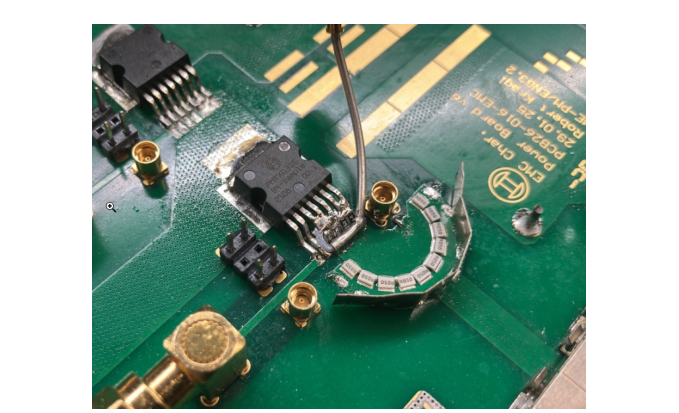
\includegraphics[scale=1]{figures/5_CurrentProbe/Diss_Pic_PShunt.pdf}
	\caption{Realization of the passive shunt for verification.}\label{fig:Diss_Pic_PShunt}
\end{figure}

As a reference, a high-ohmic shunt with \SI{250}{m\Omega} is used.
Its transfer function is shown in \fref{fig:VNA_PShunt}, where it exhibits a \mi{f}{3dB} bandwidth of \SI{385}{MHz}, which is sufficient for the low-pass verification.
The shunts are placed in the commutation loop by replacing the D2PAK source connectors with SMD shunts, while a semi-rigid coaxial SMA cable is used as the pick-up.
A photograph of the setup is shown in \fref{fig:Diss_Pic_PShunt}.

\begin{figure}[ht]
	\centering
	% This file was created by matlab2tikz.
%
%The latest updates can be retrieved from
%  http://www.mathworks.com/matlabcentral/fileexchange/22022-matlab2tikz-matlab2tikz
%where you can also make suggestions and rate matlab2tikz.
%
\definecolor{mycolor1}{rgb}{0.00000,0.44700,0.74100}%
\definecolor{mycolor2}{rgb}{0.85000,0.32500,0.09800}%
\definecolor{mycolor3}{rgb}{0.92900,0.69400,0.12500}%
\definecolor{mycolor4}{rgb}{0.49400,0.18400,0.55600}%
%
\begin{tikzpicture}

\begin{axis}[%
width=5.492in,
height=1.714in,
at={(0.921in,0.471in)},
scale only axis,
xmode=log,
xmin=0.1,
xmax=1000,
xtick={0.1,1,10,100,1000},
xticklabels={{0.1},{1},{10},{100},{1000}},
xminorticks=true,
xlabel style={font=\color{white!15!black}},
xlabel={Frequency in MHz},
ymin=-60,
ymax=0,
ylabel style={font=\color{white!15!black}},
ylabel={Magnitude in dB},
axis background/.style={fill=white},
xmajorgrids,
xminorgrids,
ymajorgrids,
grid style={dotted},
legend style={at={(0.03,0.97)}, anchor=north west, legend cell align=left, align=left, draw=white!15!black}
]
\addplot [color=mycolor1, line width=1.5pt]
  table[row sep=crcr]{%
0.1	-0.1113608229\\
0.102821974	-0.1106112179\\
0.109876909	-0.1104688438\\
0.111287897	-0.1092707728\\
0.112698884	-0.1118234825\\
0.114815364	-0.1118454559\\
0.117637338	-0.1124389545\\
0.125397767	-0.1073454512\\
0.126808754	-0.1134031677\\
0.128925235	-0.114570386\\
0.130336222	-0.1145717385\\
0.131041715	-0.1103384526\\
0.132452703	-0.1119779867\\
0.138482796	-0.1114999755\\
0.142375573	-0.1102876721\\
0.143348768	-0.112344566\\
0.144321962	-0.110082882\\
0.145295157	-0.1126451274\\
0.146268351	-0.1110470238\\
0.147241545	-0.1135906119\\
0.152107517	-0.1083605748\\
0.154053906	-0.1124386366\\
0.156000295	-0.1105633597\\
0.158919878	-0.1130287254\\
0.167678628	-0.1154593545\\
0.1725446	-0.1146949355\\
0.179356961	-0.11337945\\
0.18811571	-0.111770622\\
0.195596933	-0.1128805991\\
0.198281036	-0.1124944441\\
0.20230719	-0.1125386596\\
0.207675395	-0.1123839266\\
0.21170155	-0.1126398418\\
0.215727704	-0.113347872\\
0.218411806	-0.1115071881\\
0.221095909	-0.1125328129\\
0.242568731	-0.1133762668\\
0.245252834	-0.1155449368\\
0.253305142	-0.1144119577\\
0.260015399	-0.1149780243\\
0.261582765	-0.1129011215\\
0.265273664	-0.1149001057\\
0.268964563	-0.1140331048\\
0.283728159	-0.1145967987\\
0.285573608	-0.1159191863\\
0.289264507	-0.114789227\\
0.318791699	-0.1140271804\\
0.333555295	-0.1151040883\\
0.359701417	-0.1156497128\\
0.367338544	-0.1165967884\\
0.423344138	-0.1166936061\\
0.46152977	-0.1174553846\\
0.476804023	-0.1153271704\\
0.50111614	-0.1162749421\\
0.515158441	-0.1158437643\\
0.543243041	-0.1160138497\\
0.680155469	-0.1207899825\\
0.737524793	-0.1211927714\\
0.77142348	-0.1202581289\\
0.800479497	-0.1216259102\\
0.8634342	-0.1198948633\\
0.887647548	-0.1210627327\\
0.911860895	-0.1196112785\\
0.936074243	-0.1197332703\\
1.02004808	-0.1201004979\\
1.080151181	-0.1203331034\\
1.160288649	-0.1208881514\\
4.814599836	-0.130119183\\
5.079689667	-0.1311582886\\
5.245370812	-0.1305734169\\
5.709278018	-0.1320343714\\
12.12137946	-0.1441270454\\
12.75590504	-0.1462376729\\
14.14671793	-0.1483232934\\
16.58064048	-0.1535159975\\
18.61637613	-0.1571655397\\
19.81168941	-0.1595415421\\
26.59592024	-0.1719262518\\
29.56389918	-0.1775663608\\
33.59463202	-0.1840695569\\
38.14229053	-0.1895243698\\
41.09826856	-0.1932150493\\
47.75921134	-0.203798167\\
50.57327152	-0.207448246\\
56.51406525	-0.2172619196\\
62.66925782	-0.2262863922\\
68.27638994	-0.2352262063\\
86.68817822	-0.2527897827\\
95.61009637	-0.2647249861\\
101.5580418	-0.2754483241\\
110.4799599	-0.2970358458\\
116.7508695	-0.3166355959\\
122.4761667	-0.3423260435\\
132.2909619	-0.4002972338\\
136.38046	-0.4357698632\\
142.1057572	-0.5028596608\\
150.2847533	-0.6260888354\\
156.8279501	-0.7210592943\\
161.675471	-0.7617759064\\
163.9319773	-0.7709072932\\
166.1884837	-0.7658660937\\
169.5732432	-0.7424011749\\
174.0862559	-0.6937666048\\
192.1383066	-0.4829374434\\
198.9078257	-0.4321562403\\
204.5490915	-0.4059328285\\
214.7033701	-0.379972554\\
218.0881296	-0.3814787983\\
222.0936934	-0.3929585063\\
228.3172134	-0.4293759556\\
243.8760136	-0.523343137\\
248.5436536	-0.5208934736\\
251.6554136	-0.5353679438\\
257.8789337	-0.5645015748\\
262.5465737	-0.5733028428\\
267.2142137	-0.5796054784\\
271.8818538	-0.5928294723\\
274.9936138	-0.613489303\\
281.2171338	-0.6809797043\\
292.1082939	-0.8182771563\\
311.8457146	-1.128817165\\
313.9919762	-1.135517682\\
322.5770228	-1.121505785\\
326.8695461	-1.117490279\\
329.0158078	-1.116541881\\
333.3083311	-1.142338545\\
341.8933777	-1.230529947\\
350.4784243	-1.372425101\\
361.2097326	-1.638705342\\
374.0873025	-1.974809758\\
386.9648724	-2.085087879\\
391.2573957	-2.060538843\\
408.4274889	-1.850539442\\
412.7200122	-1.907712784\\
417.0125355	-2.042918132\\
422.486007	-2.373433983\\
440.2443915	-3.956235791\\
443.2041222	-3.989162242\\
446.163853	-3.936744867\\
466.8819682	-3.180001567\\
469.8416989	-3.18358961\\
472.8014297	-3.201017305\\
478.7208912	-3.302849188\\
496.4792757	-3.646659035\\
505.3584679	-3.731002172\\
508.3181987	-3.738016348\\
514.2376601	-3.779659596\\
520.1571216	-3.859616102\\
526.0765831	-4.039125635\\
540.8752369	-4.789228903\\
570.4725443	-5.187640222\\
576.8889099	-5.344268991\\
580.9588239	-5.336143583\\
585.0287378	-5.296303628\\
589.0986518	-5.349723605\\
605.3783076	-5.827910662\\
625.7278773	-7.021709883\\
629.7977913	-7.06793681\\
666.4270168	-5.810631166\\
686.7765866	-4.82529612\\
707.1261563	-4.303448055\\
715.2659843	-4.225291435\\
723.4058122	-4.270881908\\
727.4757261	-4.263196369\\
755.9651238	-4.574391304\\
776.3146935	-4.812197538\\
780.3846075	-4.820948941\\
788.5244354	-4.880846767\\
793.2776401	-4.961608469\\
810.1203919	-5.45482128\\
815.7346424	-5.447785864\\
832.5773941	-5.619102264\\
838.1916447	-5.613850482\\
849.4201459	-5.593566841\\
860.648647	-5.426262612\\
866.2628976	-5.39840847\\
888.7198998	-5.039172915\\
905.5626516	-4.855677208\\
916.7911527	-4.623239343\\
922.4054033	-4.637015036\\
928.0196538	-4.743127492\\
944.8624056	-5.685517709\\
961.7051573	-5.260965507\\
972.9336584	-5.212971692\\
984.1621596	-5.517507873\\
1001.004911	-6.276826078\\
};
\addlegendentry{$\mathrm{S}_\mathrm{11}$}

\addplot [color=mycolor2, line width=1.5pt]
  table[row sep=crcr]{%
0.1	-40.17843466\\
0.101410987	-40.14957287\\
0.102116481	-40.13714666\\
0.102821974	-40.22248108\\
0.103527468	-40.14279048\\
0.104232961	-40.15306646\\
0.104938455	-40.14422265\\
0.105643948	-40.10379595\\
0.106349442	-40.18747815\\
0.107054935	-40.1370117\\
0.107760429	-40.15068797\\
0.109171416	-40.1502343\\
0.109876909	-40.14101046\\
0.110582403	-40.14402163\\
0.111287897	-40.16953993\\
0.11199339	-40.1655318\\
0.112698884	-40.17225231\\
0.113404377	-40.17003459\\
0.115520858	-40.14557651\\
0.116226351	-40.18513349\\
0.117637338	-40.14575152\\
0.118342832	-40.14096041\\
0.119753819	-40.17472517\\
0.120459312	-40.17316128\\
0.121164806	-40.15725303\\
0.1218703	-40.18803398\\
0.122575793	-40.18123489\\
0.123281287	-40.16104951\\
0.124692274	-40.18311073\\
0.126103261	-40.17062657\\
0.126808754	-40.18547802\\
0.127514248	-40.15301345\\
0.128219741	-40.18077612\\
0.128925235	-40.17029635\\
0.129630728	-40.17496507\\
0.131747209	-40.15681052\\
0.132452703	-40.17510491\\
0.133158196	-40.17217735\\
0.13386369	-40.19778307\\
0.135274677	-40.16415689\\
0.136685664	-40.17587112\\
0.137509601	-40.17216422\\
0.138482796	-40.17865891\\
0.13945599	-40.16226761\\
0.140429185	-40.16808386\\
0.141402379	-40.18258126\\
0.142375573	-40.15788797\\
0.144321962	-40.18189224\\
0.145295157	-40.18178542\\
0.146268351	-40.15936497\\
0.14821474	-40.19289413\\
0.150161129	-40.17303273\\
0.152107517	-40.15180526\\
0.153080712	-40.17792863\\
0.154053906	-40.17574153\\
0.155027101	-40.18501332\\
0.156000295	-40.16920778\\
0.156973489	-40.18123101\\
0.158919878	-40.17687991\\
0.159893073	-40.19364933\\
0.160866267	-40.17860451\\
0.161839461	-40.18029065\\
0.162812656	-40.1517051\\
0.16378585	-40.17813492\\
0.165732239	-40.17127354\\
0.166705433	-40.1442627\\
0.167678628	-40.1475192\\
0.169625017	-40.17777611\\
0.171571405	-40.15400439\\
0.174490989	-40.17200655\\
0.175464183	-40.15945531\\
0.176437377	-40.17055246\\
0.177410572	-40.14715946\\
0.178383766	-40.15935314\\
0.179356961	-40.15165001\\
0.180330155	-40.16128972\\
0.181303349	-40.14542968\\
0.182276544	-40.17448969\\
0.183249738	-40.16305179\\
0.184222933	-40.17107023\\
0.186169321	-40.14163719\\
0.187142516	-40.16309846\\
0.18811571	-40.15165667\\
0.189088905	-40.16575151\\
0.190228728	-40.16040135\\
0.191570779	-40.14367621\\
0.19291283	-40.15951388\\
0.194254882	-40.15091171\\
0.199623087	-40.16065009\\
0.200965139	-40.16110234\\
0.20230719	-40.15823493\\
0.203649241	-40.14321912\\
0.204991293	-40.16340251\\
0.207675395	-40.1456019\\
0.209017447	-40.14763968\\
0.210359498	-40.16220311\\
0.21170155	-40.15045109\\
0.213043601	-40.16060264\\
0.214385652	-40.14885493\\
0.217069755	-40.16150555\\
0.221095909	-40.16094809\\
0.22243796	-40.15095312\\
0.225122063	-40.16514013\\
0.226464115	-40.17063416\\
0.229148217	-40.15422715\\
0.23183232	-40.16032832\\
0.234516423	-40.1456574\\
0.237200526	-40.17340574\\
0.24122668	-40.14939796\\
0.242568731	-40.1572823\\
0.243910782	-40.15450757\\
0.245252834	-40.16344976\\
0.249278988	-40.14784334\\
0.250621039	-40.14576938\\
0.251963091	-40.12887113\\
0.254647193	-40.16767606\\
0.258673347	-40.1339611\\
0.261582765	-40.16112109\\
0.263428214	-40.14891417\\
0.265273664	-40.15601156\\
0.267119113	-40.15055255\\
0.268964563	-40.13050742\\
0.270810012	-40.15219958\\
0.272655462	-40.13680739\\
0.274500911	-40.14661191\\
0.276346361	-40.13045696\\
0.27819181	-40.14004455\\
0.28003726	-40.13715656\\
0.281882709	-40.16064844\\
0.283728159	-40.14700234\\
0.287419058	-40.15150007\\
0.289264507	-40.14647533\\
0.291109957	-40.13166396\\
0.292955406	-40.15726136\\
0.296646305	-40.13931818\\
0.300337204	-40.15338688\\
0.302182654	-40.1499421\\
0.305873553	-40.13724783\\
0.309564452	-40.14987553\\
0.311409901	-40.14258872\\
0.313255351	-40.15068924\\
0.3151008	-40.14395866\\
0.31694625	-40.15495608\\
0.318791699	-40.14732838\\
0.320637149	-40.15435856\\
0.322482598	-40.14861012\\
0.324328048	-40.15119173\\
0.326173497	-40.1464815\\
0.328018947	-40.16231289\\
0.329864396	-40.14083471\\
0.331709845	-40.15261665\\
0.333555295	-40.14874531\\
0.335400744	-40.13916564\\
0.337246194	-40.14384606\\
0.339091643	-40.16985954\\
0.340937093	-40.13752884\\
0.342782542	-40.15588303\\
0.344627992	-40.14874324\\
0.346473441	-40.15782781\\
0.348318891	-40.13532368\\
0.35016434	-40.14277512\\
0.353855239	-40.13734202\\
0.355700689	-40.14375773\\
0.359701417	-40.14239863\\
0.362247126	-40.14973772\\
0.364792835	-40.14440907\\
0.367338544	-40.14683935\\
0.369884252	-40.15999144\\
0.372429961	-40.13180933\\
0.377521379	-40.15734371\\
0.380067088	-40.13624115\\
0.382612797	-40.15053054\\
0.385158505	-40.14511749\\
0.387704214	-40.12908107\\
0.390249923	-40.15540276\\
0.392795632	-40.14594501\\
0.395341341	-40.15034826\\
0.400432758	-40.13664645\\
0.402978467	-40.14719659\\
0.410615594	-40.13792604\\
0.415707011	-40.15554418\\
0.41825272	-40.13903466\\
0.420798429	-40.15676544\\
0.425889847	-40.14065799\\
0.428435555	-40.14422745\\
0.430981264	-40.13681132\\
0.433526973	-40.14401185\\
0.436072682	-40.13862777\\
0.438618391	-40.14034256\\
0.441164099	-40.13222539\\
0.443709808	-40.15895914\\
0.446255517	-40.13295404\\
0.453892644	-40.15198747\\
0.458984061	-40.12737167\\
0.46152977	-40.14361297\\
0.466621188	-40.14922811\\
0.471712605	-40.14246887\\
0.474258314	-40.14593654\\
0.476804023	-40.13601637\\
0.479349732	-40.13977015\\
0.481895441	-40.15419417\\
0.486986858	-40.13261781\\
0.489532567	-40.15313514\\
0.494623985	-40.12530015\\
0.497605565	-40.15782102\\
0.504626715	-40.13823081\\
0.50813729	-40.14261048\\
0.511647866	-40.14177292\\
0.515158441	-40.12904695\\
0.522179591	-40.13797929\\
0.529200741	-40.13696927\\
0.532711316	-40.14661065\\
0.539732466	-40.12918164\\
0.543243041	-40.12794969\\
0.546753616	-40.13443902\\
0.550264191	-40.12918301\\
0.553774767	-40.14596587\\
0.560795917	-40.13493316\\
0.571327642	-40.14898159\\
0.574838217	-40.12851777\\
0.581859367	-40.14506035\\
0.585369942	-40.1474262\\
0.592391092	-40.13277727\\
0.595901667	-40.11953145\\
0.606433393	-40.14438645\\
0.609943968	-40.13567975\\
0.613454543	-40.13741508\\
0.620475693	-40.13269724\\
0.627496843	-40.14106971\\
0.634517993	-40.14683772\\
0.645049719	-40.14168808\\
0.648560294	-40.13338123\\
0.652070869	-40.14428936\\
0.659092019	-40.1379138\\
0.666113169	-40.14650535\\
0.673134319	-40.13538915\\
0.676644894	-40.14322544\\
0.680155469	-40.12717892\\
0.689098098	-40.14199552\\
0.713311446	-40.14299027\\
0.722996785	-40.13073335\\
0.732682124	-40.15412948\\
0.737524793	-40.13598557\\
0.747210132	-40.1479754\\
0.756895471	-40.1338972\\
0.761738141	-40.1424693\\
0.76658081	-40.13732338\\
0.776266149	-40.14519224\\
0.781108819	-40.12932424\\
0.790794158	-40.13711161\\
0.795636827	-40.13969529\\
0.800479497	-40.13257054\\
0.805322166	-40.13471515\\
0.810164836	-40.14141339\\
0.834378183	-40.13330576\\
0.839220853	-40.14754905\\
0.844063522	-40.14550851\\
0.848906192	-40.13593666\\
0.8634342	-40.1416045\\
0.86827687	-40.13835704\\
0.877962209	-40.14519658\\
0.882804878	-40.13575059\\
0.887647548	-40.14324468\\
0.907018226	-40.13699416\\
0.911860895	-40.14673792\\
0.916703565	-40.12928007\\
0.926388904	-40.13928538\\
0.936074243	-40.13534353\\
0.940916912	-40.14003267\\
0.953266857	-40.13116876\\
0.966623102	-40.13526694\\
0.973301224	-40.13614093\\
0.986657469	-40.1421288\\
0.993335591	-40.12917864\\
1.000013714	-40.13262544\\
1.006691836	-40.14546394\\
1.02004808	-40.13659603\\
1.026726203	-40.14163691\\
1.033404325	-40.13480473\\
1.04676057	-40.15394272\\
1.066794937	-40.13297697\\
1.080151181	-40.13794273\\
1.086829304	-40.14141529\\
1.093507426	-40.13845034\\
1.100185548	-40.1499027\\
1.10686367	-40.14212965\\
1.120219915	-40.13550195\\
1.126898037	-40.14396673\\
1.13357616	-40.14145247\\
1.140254282	-40.13214723\\
1.146932404	-40.13418595\\
1.153610527	-40.14472524\\
1.160288649	-40.14171553\\
1.173644894	-40.14254996\\
1.187001138	-40.135496\\
1.200357383	-40.14322181\\
1.213713627	-40.13380476\\
1.22039175	-40.14375821\\
1.227069872	-40.13351746\\
1.233747994	-40.1472008\\
1.247104239	-40.13919785\\
1.260460484	-40.13302511\\
1.267138606	-40.13867008\\
1.273816728	-40.13277398\\
1.287172973	-40.14423268\\
1.293851095	-40.13358841\\
1.320016515	-40.15144249\\
1.338382633	-40.13011476\\
1.356748752	-40.14918631\\
1.375114871	-40.14215994\\
1.38429793	-40.14571218\\
1.393480989	-40.14451906\\
1.402664049	-40.14936\\
1.430213227	-40.12811029\\
1.439396286	-40.14125971\\
1.448579346	-40.12957017\\
1.466945464	-40.14929669\\
1.476128524	-40.13528378\\
1.494494642	-40.14553108\\
1.512860761	-40.13424564\\
1.53122688	-40.14096981\\
1.540409939	-40.1576145\\
1.549592999	-40.1343654\\
1.558776058	-40.14891792\\
1.567959117	-40.14320462\\
1.577142177	-40.14700957\\
1.595508295	-40.13007331\\
1.613874414	-40.13379059\\
1.623057473	-40.14474998\\
1.650606652	-40.13374234\\
1.66897277	-40.14228776\\
1.67815583	-40.14030352\\
1.687338889	-40.13141762\\
1.696521948	-40.14997278\\
1.705705008	-40.14140467\\
1.714888067	-40.14885205\\
1.724071126	-40.13769687\\
1.742437245	-40.14013107\\
1.760803364	-40.13828013\\
1.769986423	-40.15203211\\
1.802561859	-40.13644513\\
1.815229447	-40.14547547\\
1.827897036	-40.13485998\\
1.840564625	-40.13922492\\
1.853232214	-40.13591773\\
1.878567391	-40.14342156\\
1.89123498	-40.13398714\\
1.929237746	-40.14593271\\
1.941905335	-40.15086669\\
1.954572924	-40.13155099\\
1.967240513	-40.1426846\\
1.979908101	-40.12942276\\
1.99257569	-40.14045709\\
2.005243279	-40.1375586\\
2.017910868	-40.14715\\
2.030578457	-40.14485921\\
2.043246045	-40.15227488\\
2.068581223	-40.14293377\\
2.0939164	-40.15046118\\
2.131919167	-40.13486273\\
2.144586756	-40.14290948\\
2.169921933	-40.13894979\\
2.195257111	-40.14963087\\
2.207924699	-40.14784983\\
2.220592288	-40.13570547\\
2.245927466	-40.14219471\\
2.271262643	-40.13545009\\
2.283930232	-40.15055046\\
2.296597821	-40.13610529\\
2.30926541	-40.1463923\\
2.321932998	-40.13431713\\
2.334600587	-40.14078034\\
2.347268176	-40.13075144\\
2.359935765	-40.13577249\\
2.372603353	-40.15093661\\
2.385270942	-40.14313228\\
2.41060612	-40.14668664\\
2.423273708	-40.14004418\\
2.435941297	-40.156252\\
2.448608886	-40.14134383\\
2.493581802	-40.15186345\\
2.511050619	-40.14703864\\
2.528519436	-40.15189967\\
2.545988253	-40.14028699\\
2.580925887	-40.14591818\\
2.615863521	-40.14051714\\
2.650801155	-40.15020864\\
2.668269972	-40.13638634\\
2.685738789	-40.1439577\\
2.703207606	-40.13370542\\
2.73814524	-40.15926837\\
2.755614057	-40.14384303\\
2.790551691	-40.15081659\\
2.808020508	-40.14600869\\
2.842958142	-40.15233987\\
2.860426959	-40.14430382\\
2.877895776	-40.14556942\\
2.895364593	-40.15498514\\
2.91283341	-40.13737397\\
2.947771044	-40.15860274\\
2.965239861	-40.14236781\\
2.982708678	-40.15614658\\
3.000177495	-40.12955561\\
3.035115129	-40.15750087\\
3.087521579	-40.14663503\\
3.104990396	-40.15793297\\
3.122459213	-40.1471738\\
3.13992803	-40.15918717\\
3.157396847	-40.1401604\\
3.174865664	-40.15451208\\
3.244740932	-40.14184076\\
3.262209749	-40.15235347\\
3.297147383	-40.1417768\\
3.3146162	-40.15356658\\
3.332085017	-40.14067169\\
3.367022651	-40.15319027\\
3.384491468	-40.15078415\\
3.404893095	-40.13987783\\
3.428914395	-40.1489241\\
3.452935696	-40.14444239\\
3.476956996	-40.13379164\\
3.500978297	-40.15498443\\
3.524999597	-40.15388628\\
3.549020898	-40.14889292\\
3.573042199	-40.15208513\\
3.6210848	-40.13251199\\
3.669127401	-40.14986323\\
3.717170002	-40.13760733\\
3.765212603	-40.15376216\\
3.813255204	-40.14743009\\
3.861297806	-40.15088328\\
3.885319106	-40.1540356\\
3.933361707	-40.15042243\\
3.957383008	-40.15601466\\
4.005425609	-40.14078405\\
4.02944691	-40.16164067\\
4.05346821	-40.15116487\\
4.101510811	-40.15854006\\
4.125532112	-40.14642237\\
4.149553413	-40.1494155\\
4.197596014	-40.14046566\\
4.245638615	-40.1581879\\
4.293681216	-40.14553371\\
4.317702517	-40.1564265\\
4.341723817	-40.14344683\\
4.365745118	-40.14627291\\
4.389766418	-40.14424329\\
4.413787719	-40.15280532\\
4.43780902	-40.1414939\\
4.46183032	-40.14778967\\
4.485851621	-40.14602508\\
4.509872921	-40.15668245\\
4.533894222	-40.14671412\\
4.557915522	-40.15104252\\
4.581936823	-40.14584197\\
4.605958124	-40.15642747\\
4.629979424	-40.14645071\\
4.68205492	-40.15452002\\
4.715191149	-40.1445494\\
4.748327378	-40.16053152\\
4.847736065	-40.14118462\\
4.880872294	-40.16065897\\
4.914008523	-40.1490109\\
4.947144752	-40.15312512\\
4.980280981	-40.14821897\\
5.01341721	-40.15847643\\
5.046553439	-40.15433609\\
5.112825896	-40.15677557\\
5.145962125	-40.14177745\\
5.245370812	-40.15437959\\
5.278507041	-40.14619728\\
5.344779499	-40.16480866\\
5.377915728	-40.15111568\\
5.411051957	-40.15531901\\
5.444188186	-40.15000805\\
5.477324415	-40.15796152\\
5.543596873	-40.14671406\\
5.576733102	-40.16406199\\
5.609869331	-40.13668899\\
5.676141789	-40.15916853\\
5.742414247	-40.15845718\\
5.808686704	-40.1515013\\
5.908095391	-40.16077067\\
5.94123162	-40.15524218\\
6.007504078	-40.16205853\\
6.073776536	-40.16830308\\
6.106912765	-40.15941874\\
6.140048994	-40.16221046\\
6.173185223	-40.15480805\\
6.206321452	-40.15941911\\
6.239457681	-40.15476875\\
6.305730139	-40.16348658\\
6.372002597	-40.15234039\\
6.405138826	-40.15855367\\
6.438275055	-40.15562287\\
6.477084809	-40.16200105\\
6.522780223	-40.15081337\\
6.568475638	-40.16409115\\
6.659866467	-40.15438698\\
6.79695271	-40.16279693\\
6.842648125	-40.15173792\\
6.934038953	-40.16222536\\
6.979734368	-40.15571073\\
7.071125197	-40.16647139\\
7.116820611	-40.16832935\\
7.162516026	-40.15862968\\
7.20821144	-40.16254289\\
7.253906855	-40.15295858\\
7.299602269	-40.1690639\\
7.345297683	-40.16161292\\
7.390993098	-40.16774994\\
7.482383927	-40.156209\\
7.573774756	-40.16678998\\
7.665165585	-40.16987293\\
7.756556413	-40.16382674\\
7.847947242	-40.16861796\\
7.939338071	-40.1602427\\
7.985033486	-40.16512731\\
8.0307289	-40.16155987\\
8.122119729	-40.17176571\\
8.167815143	-40.15340436\\
8.259205972	-40.16905137\\
8.350596801	-40.1668791\\
8.396292216	-40.16101017\\
8.44198763	-40.16822693\\
8.533378459	-40.16796554\\
8.579073873	-40.179606\\
8.670464702	-40.16638524\\
8.716160117	-40.177836\\
8.761855531	-40.16535048\\
8.85324636	-40.17378595\\
8.906613499	-40.16693901\\
8.969648125	-40.17699592\\
9.095717379	-40.16512926\\
9.158752005	-40.17769726\\
9.221786632	-40.17214227\\
9.284821259	-40.17670483\\
9.347855886	-40.17580911\\
9.410890512	-40.18012816\\
9.536959766	-40.16851819\\
9.599994392	-40.17405765\\
9.726063646	-40.17077009\\
9.789098272	-40.17547606\\
9.915167526	-40.17054306\\
10.04123678	-40.17499611\\
10.10427141	-40.17154604\\
10.23034066	-40.18245159\\
10.29337529	-40.1711278\\
10.35640991	-40.18488818\\
10.48247917	-40.17324475\\
10.54551379	-40.18052928\\
10.67158305	-40.172992\\
10.7976523	-40.18329759\\
10.86068693	-40.1786333\\
10.92372155	-40.18603431\\
11.11282543	-40.17458381\\
11.17586006	-40.18637676\\
11.30192931	-40.17598351\\
11.42799857	-40.19360328\\
11.49103319	-40.1782822\\
11.55406782	-40.18687528\\
11.68013707	-40.18132102\\
11.7431717	-40.18616151\\
11.80620633	-40.18393473\\
11.86924095	-40.17470862\\
11.93227558	-40.18808874\\
11.99531021	-40.17760228\\
12.05834483	-40.18709488\\
12.12137946	-40.18143716\\
12.18441409	-40.19552706\\
12.24744871	-40.17736384\\
12.58205343	-40.20089465\\
12.75590504	-40.19142956\\
12.84283085	-40.18287668\\
12.92975665	-40.19886166\\
13.01668246	-40.18580722\\
13.19053407	-40.19299628\\
13.36438568	-40.1920896\\
13.45131149	-40.18925451\\
13.53823729	-40.19937691\\
13.6251631	-40.19502977\\
13.7120889	-40.21501113\\
13.79901471	-40.19683017\\
13.88594051	-40.19967439\\
13.97286632	-40.19474704\\
14.05979212	-40.19590902\\
14.14671793	-40.19211689\\
14.40749535	-40.20828763\\
14.49442115	-40.19608312\\
14.58134696	-40.20208637\\
14.75519857	-40.19486283\\
14.92905018	-40.20518818\\
15.01597598	-40.18914217\\
15.1898276	-40.21477782\\
15.2767534	-40.20662558\\
15.36367921	-40.21032474\\
15.53753082	-40.20166742\\
15.79830823	-40.2068265\\
15.88523404	-40.20101747\\
16.05908565	-40.21321663\\
16.23293726	-40.2054316\\
16.40678887	-40.20869168\\
16.58064048	-40.21232271\\
16.66756629	-40.2181736\\
16.94293753	-40.21187053\\
17.30153151	-40.22099137\\
17.42106284	-40.23056994\\
17.54059417	-40.21401272\\
17.77965683	-40.22108143\\
17.89918816	-40.22835821\\
18.13825081	-40.22237159\\
18.25778214	-40.23526702\\
18.37731347	-40.23330247\\
18.4968448	-40.22573626\\
18.61637613	-40.23659133\\
18.73590746	-40.22269906\\
19.3335641	-40.23835535\\
19.45309543	-40.23128728\\
19.69215808	-40.23711652\\
19.81168941	-40.24142841\\
19.93122074	-40.23257224\\
20.05075207	-40.24200084\\
20.28981473	-40.23191863\\
20.40934606	-40.24833572\\
20.76794004	-40.23606112\\
21.0070027	-40.24885596\\
21.24606536	-40.25459983\\
21.36559668	-40.2374774\\
21.48512801	-40.25573046\\
21.60465934	-40.2490771\\
21.72419067	-40.25654783\\
21.843722	-40.24537443\\
21.96325333	-40.26721783\\
22.08278466	-40.25391816\\
22.20231598	-40.26380794\\
22.32184731	-40.25553923\\
22.6804413	-40.26944104\\
22.91950396	-40.25676249\\
23.03903528	-40.26734036\\
23.15856661	-40.26293447\\
23.29816585	-40.27084251\\
23.46305357	-40.26207982\\
23.62794129	-40.27554652\\
23.79282901	-40.27599438\\
23.95771673	-40.26324617\\
24.12260444	-40.27040291\\
24.28749217	-40.26900439\\
24.45237988	-40.27219033\\
24.78215532	-40.28901239\\
24.94704304	-40.27956766\\
25.11193076	-40.28289428\\
25.27681848	-40.28064952\\
25.60659392	-40.29310416\\
26.10125708	-40.30112025\\
26.43103252	-40.30680757\\
26.59592024	-40.29178797\\
26.76080796	-40.29844128\\
26.92569568	-40.28749949\\
27.09058339	-40.31267125\\
27.25547111	-40.30065587\\
27.42035883	-40.31231848\\
27.75013427	-40.31132816\\
27.91502199	-40.32020556\\
28.07990971	-40.3082569\\
28.24479743	-40.31181682\\
28.57457287	-40.33202174\\
28.73946059	-40.3211275\\
28.90434831	-40.32294768\\
29.23412375	-40.33556738\\
29.39901147	-40.33253328\\
29.56389919	-40.33480149\\
29.7287869	-40.32372883\\
29.89367462	-40.34447868\\
30.05856234	-40.33914993\\
30.38833778	-40.34711544\\
30.5532255	-40.34469561\\
31.3776641	-40.3686096\\
31.54255182	-40.36329895\\
31.70743954	-40.36525411\\
32.23033447	-40.39357417\\
32.4577174	-40.38673197\\
32.68510032	-40.39571041\\
32.91248325	-40.38533803\\
33.13986618	-40.39549652\\
33.3672491	-40.39037276\\
33.59463203	-40.40548527\\
33.82201495	-40.40228895\\
34.04939788	-40.41657615\\
34.2767808	-40.40680325\\
34.50416373	-40.41101625\\
34.73154665	-40.42553777\\
34.95892958	-40.41784143\\
35.64107835	-40.42288529\\
35.86846128	-40.43726056\\
36.0958442	-40.43321286\\
36.32322713	-40.4391194\\
36.55061005	-40.4317961\\
36.77799298	-40.44100958\\
37.23275883	-40.44098338\\
37.46014176	-40.44785789\\
37.68752468	-40.4659622\\
37.91490761	-40.46362679\\
38.14229053	-40.45607919\\
38.59705638	-40.46456733\\
38.82443931	-40.47522702\\
39.05182223	-40.46712608\\
39.50658808	-40.47160765\\
39.73397101	-40.48705578\\
39.96135393	-40.47326014\\
40.18873686	-40.49093709\\
40.41611979	-40.47690902\\
41.32565149	-40.49862425\\
41.55303441	-40.48981655\\
42.00780026	-40.50266118\\
42.23518319	-40.49443108\\
42.68994904	-40.5034475\\
42.91733196	-40.51902777\\
43.37209781	-40.51334287\\
44.31980444	-40.53470706\\
44.94515115	-40.5252122\\
45.57049786	-40.54413347\\
45.88317121	-40.5371187\\
46.50851792	-40.5506181\\
47.13386463	-40.54847186\\
47.75921134	-40.57178884\\
48.07188469	-40.56117681\\
48.6972314	-40.57524297\\
49.32257811	-40.58669212\\
49.63525146	-40.57231566\\
49.94792482	-40.59446904\\
50.26059817	-40.57434098\\
51.51129158	-40.61365237\\
52.13663829	-40.61021226\\
52.44931165	-40.62350863\\
52.761985	-40.61790524\\
53.38733171	-40.6296376\\
54.01267842	-40.62701687\\
54.32535177	-40.64000082\\
55.26337183	-40.65095656\\
55.57604519	-40.6494252\\
55.88871854	-40.66259702\\
56.2013919	-40.65931491\\
56.51406525	-40.66191863\\
56.82673861	-40.68202811\\
57.45208531	-40.68133658\\
58.07743202	-40.69524675\\
58.39010538	-40.69291683\\
59.32812544	-40.70490077\\
59.95347215	-40.7146508\\
60.2661455	-40.70730953\\
60.9439864	-40.72167459\\
61.80662211	-40.73377858\\
62.23793996	-40.74287039\\
62.66925782	-40.74058914\\
63.10057567	-40.74592127\\
63.53189353	-40.75847241\\
63.96321139	-40.74894343\\
64.82584709	-40.76017211\\
65.25716495	-40.77198029\\
65.68848281	-40.76712357\\
66.55111852	-40.81245671\\
66.98243637	-40.80124322\\
67.84507208	-40.83100654\\
68.27638994	-40.83032189\\
69.13902565	-40.87184873\\
69.5703435	-40.86263553\\
70.00166136	-40.86555698\\
70.43297921	-40.88837561\\
70.86429707	-40.86628603\\
72.15825064	-40.90887389\\
77.3340649	-40.97473243\\
77.76538276	-40.96850745\\
79.05933632	-40.98577858\\
79.49065418	-40.97180734\\
79.92197203	-41.00736428\\
81.2159256	-41.00163548\\
81.64724345	-41.00615232\\
82.07856131	-41.01761866\\
82.94119702	-41.01844037\\
83.80383273	-41.03939352\\
84.9037946	-41.03013433\\
87.28297277	-41.06613007\\
87.87776731	-41.06151425\\
90.85174002	-41.09831952\\
91.44653457	-41.09200704\\
92.04132911	-41.09273818\\
93.2309182	-41.10387741\\
93.82571274	-41.10728987\\
94.42050728	-41.10586121\\
95.01530183	-41.11144175\\
96.20489091	-41.12666053\\
96.79968545	-41.13338015\\
97.39448	-41.1250789\\
98.58406908	-41.13488083\\
99.77365817	-41.15049073\\
100.9632473	-41.13854949\\
102.1528363	-41.15502084\\
102.7476309	-41.14609929\\
103.3424254	-41.14801559\\
103.93722	-41.15762626\\
105.1268091	-41.16023351\\
105.7216036	-41.1672126\\
106.9111927	-41.16085776\\
107.5059872	-41.17031486\\
108.1007818	-41.16378972\\
109.2903709	-41.17219337\\
110.4799599	-41.17782233\\
111.669549	-41.15675768\\
112.2643436	-41.18401478\\
112.8591381	-41.16157756\\
115.2383163	-41.17956604\\
115.9329699	-41.17522241\\
116.7508695	-41.1792926\\
119.2045683	-41.16904669\\
120.0224679	-41.17492014\\
120.8403675	-41.16662921\\
121.6582671	-41.17526607\\
122.4761667	-41.17094629\\
123.2940663	-41.17640724\\
124.9298655	-41.16397894\\
125.7477651	-41.15703924\\
127.3835643	-41.16131294\\
129.0193635	-41.14578278\\
129.8372631	-41.15428631\\
131.4730623	-41.14416635\\
132.290962	-41.14635018\\
133.9267612	-41.12879262\\
134.7446608	-41.13014002\\
135.5625604	-41.12725188\\
136.38046	-41.13108972\\
137.1983596	-41.11042678\\
138.0162592	-41.12501568\\
139.6520584	-41.12136028\\
140.469958	-41.13068057\\
141.2878576	-41.12407143\\
142.9236568	-41.14021492\\
143.7415564	-41.13787172\\
144.559456	-41.15057443\\
145.3773556	-41.1475772\\
151.9205525	-41.26306577\\
155.1921509	-41.36119591\\
159.4189647	-41.52068437\\
166.1884837	-41.7649589\\
177.4710154	-42.17703318\\
178.5992686	-42.18399533\\
180.8557749	-42.21302948\\
181.9840281	-42.21956962\\
183.1122813	-42.23769801\\
184.2405344	-42.21743759\\
187.6252939	-42.24670952\\
188.7535471	-42.23456323\\
189.8818003	-42.23617902\\
194.394813	-42.1900993\\
196.6513193	-42.15328579\\
197.7795725	-42.16123618\\
201.164332	-42.09543531\\
210.1903574	-41.94590144\\
220.5378134	-41.7284831\\
225.2054534	-41.63718466\\
231.4289735	-41.5445264\\
234.5407335	-41.50634864\\
239.2083735	-41.44534162\\
245.4318936	-41.36984215\\
250.0995336	-41.24988305\\
254.7671736	-41.28566505\\
256.3230536	-41.31743734\\
257.8789337	-41.31235371\\
262.5465737	-41.26321935\\
267.2142137	-41.15869127\\
271.8818538	-41.04364474\\
279.6612538	-40.84583379\\
284.3288938	-40.78138117\\
285.8847739	-40.78736478\\
287.4406539	-40.78203848\\
298.3318139	-40.64828683\\
301.443574	-40.67033986\\
303.260668	-40.68311466\\
309.6994529	-40.83481022\\
316.1382379	-41.00776569\\
322.5770228	-41.11869136\\
324.7232845	-41.11470484\\
333.3083311	-41.05634757\\
341.8933777	-41.00087824\\
344.0396394	-41.01407372\\
348.3321627	-40.99176296\\
350.4784243	-40.99374109\\
352.624686	-40.96261922\\
359.0634709	-40.7658257\\
361.2097326	-40.75585988\\
365.5022559	-40.80606058\\
371.9410408	-41.07577032\\
378.3798258	-41.52293796\\
386.9648724	-42.47084289\\
397.6961807	-44.53638649\\
410.5737506	-47.76380911\\
422.486007	-51.01823903\\
425.4457377	-50.50394914\\
446.163853	-42.62334739\\
455.0430452	-40.90444413\\
463.9222374	-40.24315655\\
469.8416989	-40.06027678\\
472.8014297	-40.06903025\\
475.7611604	-40.11378288\\
487.6000834	-40.57540732\\
490.5598142	-40.55547155\\
493.5195449	-40.56391448\\
499.4390064	-40.51404427\\
502.3987372	-40.52563559\\
511.2779294	-40.74626883\\
520.1571216	-41.06791647\\
523.1168524	-41.04899281\\
529.0363139	-40.83735569\\
537.9155061	-40.51651694\\
543.8349676	-40.46698129\\
558.6336214	-40.1461349\\
564.5530828	-40.073152\\
570.4725443	-40.04210466\\
573.4322751	-40.00381612\\
589.0986518	-39.36123671\\
597.2384797	-39.19630681\\
601.3083936	-39.23595794\\
613.5181355	-38.88459677\\
617.5880494	-38.94805481\\
625.7278773	-39.44800879\\
658.2871889	-43.16398096\\
674.5668447	-44.22216111\\
678.6367587	-44.14255759\\
698.9863284	-43.43814253\\
703.0562424	-43.40876399\\
707.1261563	-43.54852956\\
715.2659843	-44.24483693\\
719.3358982	-44.16758254\\
747.8252959	-42.64034106\\
760.0350377	-42.35061993\\
772.2447796	-42.16486545\\
780.3846075	-42.1974402\\
788.5244354	-42.3184397\\
804.5061413	-42.16127474\\
821.348893	-43.68766032\\
826.9631436	-44.21592963\\
832.5773941	-44.17178902\\
843.8058953	-43.52229241\\
849.4201459	-43.50704648\\
855.0343964	-43.57561315\\
860.648647	-43.75381548\\
866.2628976	-43.71405894\\
888.7198998	-44.23104987\\
894.3341504	-44.22801436\\
905.5626516	-43.77258973\\
911.1769021	-43.85194196\\
922.4054033	-45.02700108\\
933.6339044	-48.24328478\\
961.7051573	-42.78237558\\
1001.004911	-40.73237113\\
};
\addlegendentry{$\mathrm{S}_\mathrm{12}$}

\addplot [color=mycolor3, line width=1.5pt]
  table[row sep=crcr]{%
0.1	-40.13672969\\
0.101410987	-40.20213107\\
0.102116481	-40.17188952\\
0.102821974	-40.19882024\\
0.103527468	-40.13244592\\
0.104232961	-40.19822259\\
0.104938455	-40.18028155\\
0.105643948	-40.23235271\\
0.107760429	-40.17477706\\
0.109171416	-40.21216485\\
0.109876909	-40.17114398\\
0.110582403	-40.20567223\\
0.111287897	-40.17576097\\
0.11199339	-40.2342252\\
0.112698884	-40.20170176\\
0.113404377	-40.21482276\\
0.114109871	-40.20911863\\
0.115520858	-40.21576977\\
0.116226351	-40.18819294\\
0.116931845	-40.21182588\\
0.118342832	-40.19108455\\
0.119753819	-40.21585347\\
0.120459312	-40.21130558\\
0.121164806	-40.19443959\\
0.122575793	-40.24488257\\
0.123281287	-40.19708601\\
0.12398678	-40.23400146\\
0.124692274	-40.21222091\\
0.125397767	-40.21890247\\
0.126808754	-40.19573652\\
0.127514248	-40.24397142\\
0.128219741	-40.20706291\\
0.128925235	-40.23798507\\
0.129630728	-40.21679107\\
0.130336222	-40.22848406\\
0.131041715	-40.20222051\\
0.131747209	-40.24079719\\
0.132452703	-40.20679089\\
0.133158196	-40.23251164\\
0.13386369	-40.21805198\\
0.134569183	-40.23124973\\
0.135274677	-40.22520861\\
0.13598017	-40.23213146\\
0.136685664	-40.19644406\\
0.137509601	-40.23547585\\
0.138482796	-40.23282196\\
0.13945599	-40.21948141\\
0.141402379	-40.22443386\\
0.143348768	-40.20718163\\
0.144321962	-40.20815792\\
0.146268351	-40.2471779\\
0.14821474	-40.22931731\\
0.149187934	-40.24728155\\
0.150161129	-40.24389907\\
0.152107517	-40.22810375\\
0.153080712	-40.24265085\\
0.154053906	-40.2105596\\
0.156000295	-40.24357499\\
0.158919878	-40.22605096\\
0.159893073	-40.24329223\\
0.160866267	-40.22298198\\
0.161839461	-40.22758612\\
0.164759045	-40.21378741\\
0.167678628	-40.2455758\\
0.169625017	-40.22551516\\
0.171571405	-40.23843377\\
0.1725446	-40.23344131\\
0.173517794	-40.24039639\\
0.175464183	-40.23068919\\
0.176437377	-40.23997637\\
0.181303349	-40.19921568\\
0.182276544	-40.20844127\\
0.183249738	-40.22932502\\
0.184222933	-40.21304804\\
0.186169321	-40.22296433\\
0.187142516	-40.2156352\\
0.18811571	-40.22660106\\
0.190228728	-40.21591521\\
0.191570779	-40.22008256\\
0.19291283	-40.21746817\\
0.194254882	-40.20575593\\
0.195596933	-40.22461837\\
0.198281036	-40.20468795\\
0.199623087	-40.20441997\\
0.200965139	-40.23373315\\
0.203649241	-40.19612168\\
0.204991293	-40.22660542\\
0.206333344	-40.22043692\\
0.207675395	-40.20165006\\
0.210359498	-40.20910208\\
0.21170155	-40.22165292\\
0.213043601	-40.19723285\\
0.214385652	-40.20587697\\
0.217069755	-40.19269577\\
0.219753858	-40.22224101\\
0.22243796	-40.19616235\\
0.223780012	-40.20780728\\
0.225122063	-40.20647518\\
0.226464115	-40.1992429\\
0.227806166	-40.20910438\\
0.230490269	-40.1993074\\
0.23183232	-40.20452063\\
0.234516423	-40.19501076\\
0.237200526	-40.20107651\\
0.238542577	-40.19509163\\
0.239884628	-40.21238379\\
0.24122668	-40.18251988\\
0.242568731	-40.20569443\\
0.245252834	-40.18421039\\
0.247936937	-40.20774223\\
0.250621039	-40.18655754\\
0.253305142	-40.2058331\\
0.258673347	-40.18542898\\
0.261582765	-40.19405621\\
0.263428214	-40.19182623\\
0.265273664	-40.20113923\\
0.267119113	-40.18731631\\
0.270810012	-40.1938919\\
0.272655462	-40.18511438\\
0.274500911	-40.18691431\\
0.27819181	-40.18265166\\
0.28003726	-40.17429996\\
0.281882709	-40.17858495\\
0.283728159	-40.1746379\\
0.285573608	-40.20223635\\
0.287419058	-40.18590518\\
0.289264507	-40.18679432\\
0.291109957	-40.18160247\\
0.292955406	-40.19150448\\
0.296646305	-40.16126143\\
0.300337204	-40.1858435\\
0.302182654	-40.17918145\\
0.304028103	-40.19472926\\
0.307719002	-40.17437069\\
0.309564452	-40.17012116\\
0.311409901	-40.17869792\\
0.3151008	-40.1712331\\
0.31694625	-40.18830405\\
0.318791699	-40.17393106\\
0.320637149	-40.18334779\\
0.322482598	-40.17479749\\
0.324328048	-40.18231118\\
0.326173497	-40.17286077\\
0.328018947	-40.17871318\\
0.331709845	-40.16155985\\
0.333555295	-40.17677871\\
0.335400744	-40.16000801\\
0.339091643	-40.17800901\\
0.340937093	-40.16820367\\
0.342782542	-40.17984649\\
0.344627992	-40.17007572\\
0.346473441	-40.17324511\\
0.348318891	-40.16304025\\
0.35200979	-40.17729587\\
0.355700689	-40.16588436\\
0.357546138	-40.17468987\\
0.359701417	-40.17243919\\
0.362247126	-40.15183991\\
0.364792835	-40.16681343\\
0.367338544	-40.16264349\\
0.369884252	-40.16842483\\
0.372429961	-40.16404154\\
0.37497567	-40.15418279\\
0.377521379	-40.16772222\\
0.380067088	-40.16084461\\
0.382612797	-40.16621006\\
0.385158505	-40.1580401\\
0.387704214	-40.16960831\\
0.392795632	-40.16361586\\
0.395341341	-40.17038833\\
0.400432758	-40.15689074\\
0.402978467	-40.16397551\\
0.405524176	-40.16221009\\
0.408069885	-40.14095564\\
0.410615594	-40.16214773\\
0.415707011	-40.1530737\\
0.41825272	-40.15162201\\
0.423344138	-40.15500815\\
0.425889847	-40.14368722\\
0.428435555	-40.15125087\\
0.430981264	-40.14626586\\
0.433526973	-40.14815719\\
0.436072682	-40.142507\\
0.438618391	-40.15480536\\
0.441164099	-40.1381386\\
0.443709808	-40.1517365\\
0.448801226	-40.13554811\\
0.451346935	-40.15652354\\
0.453892644	-40.14356169\\
0.458984061	-40.15071019\\
0.466621188	-40.13968234\\
0.471712605	-40.13947866\\
0.476804023	-40.15359049\\
0.479349732	-40.14466985\\
0.481895441	-40.15190603\\
0.486986858	-40.14096369\\
0.489532567	-40.15203201\\
0.492078276	-40.14831648\\
0.497605565	-40.15285286\\
0.50111614	-40.14473659\\
0.518669016	-40.15198932\\
0.522179591	-40.13650384\\
0.525690166	-40.148556\\
0.529200741	-40.1326317\\
0.532711316	-40.16110851\\
0.539732466	-40.14214428\\
0.543243041	-40.14569601\\
0.546753616	-40.12897282\\
0.550264191	-40.14295052\\
0.557285342	-40.13115243\\
0.560795917	-40.13191182\\
0.564306492	-40.14145618\\
0.567817067	-40.13322698\\
0.571327642	-40.14363307\\
0.578348792	-40.13524754\\
0.581859367	-40.149525\\
0.585369942	-40.13741617\\
0.588880517	-40.1386138\\
0.592391092	-40.14656522\\
0.599412243	-40.12213062\\
0.602922818	-40.14220239\\
0.606433393	-40.13316491\\
0.613454543	-40.13978512\\
0.620475693	-40.1405823\\
0.623986268	-40.14588614\\
0.627496843	-40.14303006\\
0.631007418	-40.13342117\\
0.638028568	-40.14445022\\
0.645049719	-40.13562903\\
0.648560294	-40.13877101\\
0.652070869	-40.13687728\\
0.655581444	-40.12620884\\
0.662602594	-40.13305468\\
0.666113169	-40.15109247\\
0.673134319	-40.12977244\\
0.676644894	-40.14169516\\
0.680155469	-40.13550567\\
0.693940768	-40.14346845\\
0.708468776	-40.14012642\\
0.713311446	-40.13315405\\
0.718154115	-40.14111821\\
0.722996785	-40.13604651\\
0.727839454	-40.15136586\\
0.732682124	-40.13688588\\
0.737524793	-40.14086984\\
0.742367463	-40.1302915\\
0.752052802	-40.12920883\\
0.756895471	-40.14282163\\
0.76658081	-40.14057731\\
0.77142348	-40.15212505\\
0.776266149	-40.13637549\\
0.785951488	-40.13743264\\
0.795636827	-40.14127904\\
0.800479497	-40.13706826\\
0.805322166	-40.13852068\\
0.810164836	-40.12349579\\
0.815007505	-40.14630646\\
0.819850175	-40.1393601\\
0.824692844	-40.14480858\\
0.829535514	-40.13853334\\
0.834378183	-40.14259881\\
0.839220853	-40.13327967\\
0.848906192	-40.14019412\\
0.853748861	-40.14527463\\
0.858591531	-40.13864415\\
0.86827687	-40.14247284\\
0.877962209	-40.13481702\\
0.887647548	-40.12895984\\
0.892490217	-40.13617549\\
0.902175556	-40.12701574\\
0.911860895	-40.13760226\\
0.926388904	-40.14628485\\
0.940916912	-40.12891172\\
0.946588735	-40.13610589\\
0.966623102	-40.13374253\\
0.979979347	-40.13513527\\
0.986657469	-40.14183309\\
1.000013714	-40.1359832\\
1.013369958	-40.14321932\\
1.026726203	-40.13401831\\
1.040082447	-40.14073789\\
1.066794937	-40.13893917\\
1.073473059	-40.13267458\\
1.086829304	-40.14059268\\
1.100185548	-40.13427433\\
1.113541793	-40.14429034\\
1.126898037	-40.13047115\\
1.140254282	-40.14455542\\
1.153610527	-40.12958274\\
1.160288649	-40.12704676\\
1.173644894	-40.13960761\\
1.187001138	-40.13729488\\
1.19367926	-40.14027001\\
1.200357383	-40.13105859\\
1.207035505	-40.1399427\\
1.213713627	-40.13747074\\
1.22039175	-40.14409195\\
1.233747994	-40.13096641\\
1.247104239	-40.14059387\\
1.253782361	-40.13662443\\
1.260460484	-40.1443964\\
1.28049485	-40.1380212\\
1.287172973	-40.13236985\\
1.293851095	-40.14899925\\
1.310833455	-40.13486809\\
1.320016515	-40.15080946\\
1.329199574	-40.13760661\\
1.347565693	-40.14566681\\
1.356748752	-40.13839264\\
1.38429793	-40.14145095\\
1.393480989	-40.13434114\\
1.402664049	-40.1443893\\
1.411847108	-40.14285463\\
1.421030167	-40.1311395\\
1.430213227	-40.14827475\\
1.457762405	-40.1310369\\
1.476128524	-40.13479509\\
1.485311583	-40.14498532\\
1.494494642	-40.13473322\\
1.512860761	-40.14443103\\
1.53122688	-40.13510235\\
1.549592999	-40.14492078\\
1.577142177	-40.13608323\\
1.604691355	-40.13931449\\
1.623057473	-40.14578898\\
1.641423592	-40.13645931\\
1.659789711	-40.14812829\\
1.66897277	-40.14371092\\
1.67815583	-40.15329226\\
1.696521948	-40.13615171\\
1.705705008	-40.14042127\\
1.724071126	-40.1374499\\
1.733254186	-40.1455734\\
1.751620305	-40.14179562\\
1.760803364	-40.13039497\\
1.769986423	-40.15110974\\
1.779169483	-40.14713555\\
1.78989427	-40.13089446\\
1.815229447	-40.13685263\\
1.827897036	-40.13220821\\
1.840564625	-40.15124623\\
1.853232214	-40.13736902\\
1.865899803	-40.14281223\\
1.878567391	-40.13287481\\
1.89123498	-40.14915942\\
1.916570158	-40.13739909\\
1.941905335	-40.15370597\\
1.967240513	-40.13926291\\
1.979908101	-40.14810505\\
1.99257569	-40.1402276\\
2.005243279	-40.14260668\\
2.017910868	-40.15094871\\
2.055913634	-40.12986025\\
2.068581223	-40.13289009\\
2.0939164	-40.14099472\\
2.106583989	-40.13521811\\
2.119251578	-40.1536645\\
2.144586756	-40.14138871\\
2.157254344	-40.14509968\\
2.169921933	-40.14245063\\
2.195257111	-40.15145801\\
2.233259877	-40.14283176\\
2.258595054	-40.15035798\\
2.271262643	-40.14819517\\
2.283930232	-40.15328305\\
2.296597821	-40.13538023\\
2.30926541	-40.14996123\\
2.334600587	-40.13586729\\
2.359935765	-40.13965166\\
2.385270942	-40.136718\\
2.41060612	-40.14815352\\
2.423273708	-40.13151329\\
2.435941297	-40.13598162\\
2.461276475	-40.15451313\\
2.476112985	-40.13839914\\
2.493581802	-40.1379404\\
2.528519436	-40.15109311\\
2.545988253	-40.13947874\\
2.56345707	-40.14991716\\
2.580925887	-40.13807555\\
2.615863521	-40.14432734\\
2.633332338	-40.15007578\\
2.668269972	-40.14494578\\
2.685738789	-40.15363252\\
2.720676423	-40.14268087\\
2.808020508	-40.15172002\\
2.825489325	-40.1462818\\
2.860426959	-40.1498696\\
2.895364593	-40.1382467\\
2.930302227	-40.15173336\\
2.947771044	-40.13984583\\
2.965239861	-40.14755265\\
2.982708678	-40.14238243\\
3.000177495	-40.14559161\\
3.017646312	-40.15628965\\
3.052583946	-40.13559509\\
3.087521579	-40.14034244\\
3.122459213	-40.13819768\\
3.13992803	-40.15211184\\
3.157396847	-40.14641038\\
3.174865664	-40.1488353\\
3.192334481	-40.16257837\\
3.227272115	-40.14907178\\
3.244740932	-40.15099367\\
3.297147383	-40.14518762\\
3.332085017	-40.154105\\
3.349553834	-40.13736266\\
3.367022651	-40.16446991\\
3.404893095	-40.14622396\\
3.428914395	-40.15021886\\
3.452935696	-40.14493086\\
3.476956996	-40.15315773\\
3.524999597	-40.14721388\\
3.549020898	-40.15247468\\
3.573042199	-40.13744672\\
3.597063499	-40.16407115\\
3.6210848	-40.14673019\\
3.6451061	-40.15693309\\
3.669127401	-40.14772554\\
3.693148702	-40.15482365\\
3.741191303	-40.14813088\\
3.837276505	-40.15160726\\
3.861297806	-40.14928249\\
3.885319106	-40.13560078\\
3.957383008	-40.1516216\\
4.005425609	-40.1553308\\
4.077489511	-40.14105315\\
4.125532112	-40.16447142\\
4.173574713	-40.15184299\\
4.245638615	-40.15302476\\
4.269659915	-40.15663271\\
4.293681216	-40.16725679\\
4.341723817	-40.14697611\\
4.413787719	-40.1535057\\
4.46183032	-40.14423744\\
4.485851621	-40.15410884\\
4.509872921	-40.15027605\\
4.533894222	-40.16167456\\
4.557915522	-40.15155767\\
4.581936823	-40.16268004\\
4.605958124	-40.14936749\\
4.654000725	-40.16670069\\
4.68205492	-40.14978386\\
4.715191149	-40.15357631\\
4.781463607	-40.14803861\\
4.814599836	-40.1544236\\
4.847736065	-40.15092373\\
4.880872294	-40.15504089\\
4.914008523	-40.14384892\\
4.947144752	-40.14787228\\
4.980280981	-40.15724164\\
5.01341721	-40.14671548\\
5.079689667	-40.16175607\\
5.112825896	-40.16524849\\
5.212234583	-40.15235028\\
5.245370812	-40.15141949\\
5.278507041	-40.16160913\\
5.31164327	-40.15162906\\
5.344779499	-40.15842279\\
5.377915728	-40.15569116\\
5.411051957	-40.14732952\\
5.444188186	-40.16294712\\
5.510460644	-40.15475449\\
5.543596873	-40.15321782\\
5.576733102	-40.1576679\\
5.609869331	-40.16912102\\
5.64300556	-40.14993969\\
5.676141789	-40.15341446\\
5.709278018	-40.16313268\\
5.808686704	-40.14852357\\
5.908095391	-40.16959612\\
5.94123162	-40.15709464\\
6.007504078	-40.16387088\\
6.040640307	-40.15501249\\
6.140048994	-40.16297774\\
6.173185223	-40.14912563\\
6.206321452	-40.16768889\\
6.239457681	-40.14777334\\
6.27259391	-40.15027144\\
6.338866368	-40.16468025\\
6.372002597	-40.16953566\\
6.438275055	-40.16093293\\
6.477084809	-40.16791073\\
6.522780223	-40.16788083\\
6.568475638	-40.16410729\\
6.614171052	-40.16684557\\
6.705561881	-40.1573768\\
6.751257296	-40.16354475\\
6.79695271	-40.15952975\\
6.842648125	-40.16086408\\
6.888343539	-40.16533339\\
6.934038953	-40.14858428\\
7.025429782	-40.16801363\\
7.116820611	-40.15650504\\
7.20821144	-40.16413089\\
7.253906855	-40.15808317\\
7.299602269	-40.16600003\\
7.436688512	-40.16299874\\
7.482383927	-40.16455748\\
7.528079341	-40.15860017\\
7.61947017	-40.16677965\\
7.710860999	-40.16004893\\
7.756556413	-40.17265535\\
7.847947242	-40.15783837\\
7.939338071	-40.17169306\\
7.985033486	-40.15837423\\
8.0307289	-40.1729372\\
8.167815143	-40.16440614\\
8.213510558	-40.16268982\\
8.259205972	-40.16754421\\
8.304901387	-40.16373077\\
8.396292216	-40.17224333\\
8.44198763	-40.17585735\\
8.533378459	-40.16517374\\
8.670464702	-40.17455441\\
8.716160117	-40.15614836\\
8.807550946	-40.17585726\\
8.906613499	-40.16782897\\
8.969648125	-40.17962862\\
9.095717379	-40.16730619\\
9.158752005	-40.16948273\\
9.284821259	-40.17478886\\
9.410890512	-40.18175281\\
9.473925139	-40.17497509\\
9.536959766	-40.17554645\\
9.599994392	-40.17199148\\
9.663029019	-40.17470862\\
9.789098272	-40.18321009\\
9.852132899	-40.17068497\\
9.915167526	-40.1740539\\
9.978202153	-40.17199892\\
10.04123678	-40.17545509\\
10.10427141	-40.17122644\\
10.16730603	-40.18707547\\
10.23034066	-40.1754833\\
10.29337529	-40.18863138\\
10.35640991	-40.17064711\\
10.41944454	-40.18175798\\
10.54551379	-40.17790197\\
10.67158305	-40.18300833\\
10.7976523	-40.1669012\\
10.92372155	-40.19169549\\
11.04979081	-40.17526441\\
11.11282543	-40.1869209\\
11.17586006	-40.17405921\\
11.23889469	-40.18069613\\
11.30192931	-40.1760818\\
11.36496394	-40.19037319\\
11.42799857	-40.18191279\\
11.68013707	-40.17827523\\
11.80620633	-40.18508201\\
11.86924095	-40.17891881\\
11.93227558	-40.19502437\\
11.99531021	-40.17800028\\
12.05834483	-40.17982722\\
12.12137946	-40.19221527\\
12.24744871	-40.18562836\\
12.32127602	-40.19190728\\
12.40820182	-40.18093808\\
12.49512763	-40.19426663\\
12.66897924	-40.18550533\\
12.84283085	-40.19196701\\
13.01668246	-40.19344691\\
13.10360827	-40.19299331\\
13.19053407	-40.1881036\\
13.27745988	-40.201719\\
13.36438568	-40.19240503\\
13.53823729	-40.20224757\\
13.6251631	-40.20469985\\
13.79901471	-40.19271999\\
13.88594051	-40.1999301\\
14.14671793	-40.19538526\\
14.23364374	-40.20748236\\
14.40749535	-40.20204592\\
14.49442115	-40.20783819\\
14.66827276	-40.20276394\\
14.84212437	-40.2120554\\
14.92905018	-40.20484901\\
15.10290179	-40.21294191\\
15.1898276	-40.20747111\\
15.36367921	-40.21308588\\
15.53753082	-40.19998909\\
15.79830823	-40.20798119\\
15.97215984	-40.20498653\\
16.05908565	-40.21280756\\
16.23293726	-40.21655643\\
16.31986307	-40.20539745\\
16.49371468	-40.20831687\\
16.58064048	-40.21811727\\
16.75449209	-40.20811783\\
16.94293753	-40.21523693\\
17.06246886	-40.21496185\\
17.18200018	-40.21999344\\
17.30153151	-40.21110031\\
17.42106284	-40.22696135\\
17.54059417	-40.22404004\\
17.6601255	-40.22927985\\
17.89918816	-40.22336301\\
18.01871948	-40.22184926\\
18.13825081	-40.23163253\\
18.73590746	-40.23035959\\
18.85543879	-40.23103211\\
18.97497011	-40.24433108\\
19.21403277	-40.23160033\\
19.3335641	-40.24467479\\
19.45309543	-40.23328479\\
19.57262676	-40.23861643\\
19.69215808	-40.23418762\\
19.93122074	-40.24148494\\
20.05075207	-40.23677315\\
20.1702834	-40.2385634\\
20.28981473	-40.2329788\\
20.40934606	-40.24741295\\
20.52887738	-40.24194095\\
20.76794004	-40.25142863\\
20.88747137	-40.24404515\\
21.48512801	-40.2601792\\
21.60465934	-40.24813708\\
21.72419067	-40.256253\\
21.843722	-40.24854876\\
21.96325333	-40.26347799\\
22.20231598	-40.25617659\\
22.44137864	-40.26890606\\
22.6804413	-40.2556149\\
22.91950396	-40.27244506\\
23.15856661	-40.26075595\\
23.46305357	-40.2764501\\
23.79282901	-40.2657946\\
24.28749217	-40.28158023\\
24.6172676	-40.27901526\\
24.78215532	-40.29488565\\
24.94704304	-40.27597101\\
25.27681848	-40.29826188\\
25.4417062	-40.2988554\\
25.60659392	-40.29043742\\
25.77148164	-40.30370027\\
26.10125708	-40.29933157\\
26.2661448	-40.30556974\\
26.43103252	-40.29598436\\
26.76080796	-40.30825225\\
26.92569568	-40.30186345\\
27.09058339	-40.30940155\\
27.42035883	-40.30446896\\
27.75013427	-40.3227619\\
28.07990971	-40.3205696\\
28.24479743	-40.31330368\\
28.73946059	-40.33380784\\
28.90434831	-40.32314662\\
29.39901147	-40.33742062\\
29.56389919	-40.33373011\\
29.89367462	-40.34755328\\
30.22345006	-40.35356415\\
30.38833778	-40.34889814\\
30.88300094	-40.35548518\\
31.04788866	-40.36399073\\
31.54255182	-40.36979089\\
31.87232726	-40.36327151\\
32.23033447	-40.37458387\\
32.4577174	-40.36482061\\
33.13986618	-40.39929906\\
33.3672491	-40.39420864\\
33.82201495	-40.39892659\\
34.2767808	-40.4171605\\
34.50416373	-40.40108808\\
34.95892958	-40.4204825\\
35.1863125	-40.41860989\\
35.41369543	-40.42976908\\
35.64107835	-40.4243172\\
35.86846128	-40.43265588\\
36.0958442	-40.43147897\\
37.23275883	-40.44809342\\
37.46014176	-40.45711369\\
37.68752468	-40.4453575\\
38.14229053	-40.45534057\\
38.59705638	-40.46488192\\
39.05182223	-40.46060215\\
39.50658808	-40.48890515\\
39.96135393	-40.46385277\\
40.41611979	-40.49333904\\
40.64350271	-40.48666208\\
40.87088564	-40.49745811\\
41.09826856	-40.48654274\\
42.00780026	-40.49750247\\
42.23518319	-40.49417296\\
43.14471489	-40.51762904\\
43.37209781	-40.50416561\\
43.82686366	-40.52691941\\
44.05424659	-40.5199846\\
44.31980444	-40.52791917\\
44.6324778	-40.52029991\\
45.2578245	-40.53891724\\
45.57049786	-40.53065275\\
45.88317121	-40.54080805\\
46.19584457	-40.53848055\\
46.82119127	-40.55276005\\
47.75921134	-40.5599652\\
48.38455804	-40.58779964\\
48.6972314	-40.56734229\\
49.00990475	-40.58476292\\
49.32257811	-40.57383638\\
49.94792482	-40.58805146\\
50.26059817	-40.58972581\\
51.19861823	-40.61112461\\
51.51129158	-40.60925388\\
51.82396494	-40.62251109\\
52.13663829	-40.61032556\\
53.07465836	-40.62379337\\
53.38733171	-40.62175701\\
53.70000506	-40.63091672\\
54.32535177	-40.64091139\\
54.63802513	-40.63878093\\
55.57604519	-40.66171376\\
55.88871854	-40.65741048\\
57.13941196	-40.67657518\\
57.45208531	-40.66726835\\
58.07743202	-40.69106832\\
58.70277873	-40.68940152\\
59.32812544	-40.71246408\\
59.64079879	-40.70476749\\
59.95347215	-40.70820755\\
60.57881885	-40.72329011\\
62.23793996	-40.7362795\\
64.39452924	-40.76523903\\
64.82584709	-40.76199107\\
65.68848281	-40.78017525\\
66.55111852	-40.79315678\\
66.98243637	-40.81786615\\
67.41375423	-40.80970368\\
69.5703435	-40.86487154\\
70.00166136	-40.86675467\\
70.86429707	-40.88917735\\
71.29561493	-40.89675773\\
71.72693278	-40.89051505\\
73.4522042	-40.93455593\\
73.88352206	-40.92893722\\
75.17747562	-40.95713992\\
76.04011133	-40.95150953\\
76.90274704	-40.97494594\\
77.3340649	-40.97714984\\
77.76538276	-40.97479001\\
78.19670061	-40.97893456\\
78.62801846	-40.99508782\\
79.05933632	-40.98654019\\
79.92197203	-41.00326974\\
81.2159256	-41.01266477\\
82.50987916	-41.0411528\\
82.94119702	-41.02802271\\
83.80383273	-41.04911944\\
84.30900005	-41.03761099\\
86.68817822	-41.06612773\\
87.28297277	-41.07911168\\
87.87776731	-41.07900141\\
88.47256185	-41.07261717\\
89.0673564	-41.08722426\\
89.66215094	-41.08703978\\
90.25694548	-41.10793928\\
90.85174002	-41.10564106\\
91.44653457	-41.11827666\\
92.04132911	-41.10888198\\
92.63612365	-41.11380504\\
93.2309182	-41.11102103\\
95.61009637	-41.14162688\\
96.20489091	-41.13354864\\
97.39448	-41.15078073\\
98.58406908	-41.14496594\\
99.17886362	-41.15478136\\
99.77365817	-41.14295016\\
100.3684527	-41.15699585\\
100.9632473	-41.14860758\\
102.1528363	-41.16665353\\
102.7476309	-41.16451359\\
103.3424254	-41.158449\\
104.5320145	-41.17670272\\
105.1268091	-41.17173742\\
105.7216036	-41.17555208\\
106.9111927	-41.16535919\\
107.5059872	-41.15921211\\
108.1007818	-41.17972984\\
109.2903709	-41.17041915\\
110.4799599	-41.16923281\\
111.0747545	-41.17849924\\
111.669549	-41.16874552\\
112.2643436	-41.17946241\\
113.4539327	-41.17562076\\
115.2383163	-41.17908973\\
115.9329699	-41.17346476\\
116.7508695	-41.18325989\\
117.5687691	-41.17492937\\
118.3866687	-41.18173669\\
120.0224679	-41.17120905\\
121.6582671	-41.17526356\\
122.4761667	-41.18094518\\
123.2940663	-41.16073927\\
124.1119659	-41.17399539\\
125.7477651	-41.15018505\\
129.8372631	-41.14401443\\
130.6551627	-41.15100597\\
133.9267612	-41.12537948\\
134.7446608	-41.13514304\\
135.5625604	-41.11518629\\
137.1983596	-41.12319101\\
138.0162592	-41.12618072\\
138.8341588	-41.1191586\\
139.6520584	-41.12821431\\
140.469958	-41.11965511\\
142.1057572	-41.13780258\\
142.9236568	-41.13078065\\
143.7415564	-41.1368916\\
145.3773556	-41.15777436\\
147.8310544	-41.17157714\\
151.1026529	-41.24267336\\
157.6458497	-41.44929446\\
160.5472178	-41.57846697\\
177.4710154	-42.18490154\\
178.5992686	-42.19057767\\
180.8557749	-42.23045968\\
181.9840281	-42.23843967\\
183.1122813	-42.23733645\\
184.2405344	-42.25591513\\
188.7535471	-42.24403054\\
189.8818003	-42.23159797\\
191.0100535	-42.24475132\\
196.6513193	-42.17294316\\
197.7795725	-42.16681656\\
202.2925852	-42.08154274\\
203.4208383	-42.07073323\\
206.8055979	-42.00247085\\
207.933851	-41.99541416\\
212.4468637	-41.90761412\\
215.8316232	-41.83564729\\
231.4289735	-41.51128205\\
232.9848535	-41.51356601\\
239.2083735	-41.4077146\\
240.7642535	-41.40941456\\
248.5436536	-41.27030125\\
250.0995336	-41.23754097\\
251.6554136	-41.24513535\\
254.7671736	-41.28486707\\
259.4348137	-41.29829885\\
274.9936138	-40.95044235\\
281.2171338	-40.82546775\\
287.4406539	-40.79075266\\
290.5524139	-40.76517412\\
298.3318139	-40.68015884\\
301.443574	-40.70407088\\
305.4069296	-40.76664144\\
313.9919762	-40.98785142\\
318.2844995	-41.05854944\\
320.4307612	-41.08274304\\
322.5770228	-41.08044259\\
324.7232845	-41.09315912\\
331.1620695	-41.0380861\\
335.4545928	-40.97663695\\
352.624686	-40.83425685\\
359.0634709	-40.67762888\\
363.3559942	-40.71362112\\
367.6485175	-40.82226074\\
374.0873025	-41.19086918\\
382.6723491	-41.98173791\\
389.1111341	-42.85692727\\
404.1349656	-46.158841\\
422.486007	-51.12231766\\
425.4457377	-50.5629542\\
446.163853	-42.38994905\\
455.0430452	-40.73264355\\
463.9222374	-40.14037071\\
469.8416989	-40.0195851\\
472.8014297	-40.05591463\\
478.7208912	-40.28543874\\
487.6000834	-40.74766088\\
493.5195449	-40.77392174\\
499.4390064	-40.70216961\\
505.3584679	-40.73471962\\
520.1571216	-41.02495271\\
523.1168524	-40.97976689\\
549.7544291	-40.01348147\\
555.6738906	-39.92053631\\
564.5530828	-39.96137027\\
570.4725443	-40.02733618\\
576.8889099	-39.98670131\\
589.0986518	-39.51695594\\
597.2384797	-39.34293921\\
601.3083936	-39.35777817\\
613.5181355	-38.8680897\\
617.5880494	-38.88911322\\
625.7278773	-39.26236754\\
670.4969308	-44.12322298\\
678.6367587	-44.4015053\\
682.7066726	-44.30520093\\
686.7765866	-44.02522166\\
690.8465005	-44.02965114\\
694.9164145	-43.97936331\\
703.0562424	-43.70212025\\
707.1261563	-43.77143229\\
715.2659843	-44.16701521\\
723.4058122	-43.67965728\\
739.685468	-42.43870283\\
747.8252959	-42.34970154\\
755.9651238	-42.25259047\\
760.0350377	-42.30146689\\
768.1748656	-42.18070237\\
780.3846075	-42.30522458\\
788.5244354	-42.51223393\\
798.8918907	-42.35737313\\
804.5061413	-42.33981713\\
810.1203919	-42.50737019\\
826.9631436	-44.06125783\\
832.5773941	-43.96452863\\
843.8058953	-43.20443943\\
849.4201459	-43.14442398\\
855.0343964	-43.21019343\\
866.2628976	-43.59585339\\
877.4913987	-43.83868444\\
894.3341504	-44.36647409\\
905.5626516	-44.25841262\\
911.1769021	-44.40244083\\
922.4054033	-45.80170426\\
933.6339044	-49.08708171\\
956.0909067	-43.26143467\\
995.3906607	-41.22547473\\
1001.004911	-41.15156605\\
};
\addlegendentry{$\mathrm{S}_\mathrm{21}$}

\addplot [color=mycolor4, line width=1.5pt]
  table[row sep=crcr]{%
0.1	-0.09602694343\\
0.113404377	-0.09675424343\\
0.114815364	-0.09712535295\\
0.116226351	-0.09777145898\\
0.118342832	-0.09910995484\\
0.122575793	-0.09789825381\\
0.12398678	-0.09910077164\\
0.135274677	-0.09817954213\\
0.147241545	-0.09795992246\\
0.14821474	-0.100243873\\
0.150161129	-0.09825123345\\
0.152107517	-0.09851322088\\
0.155027101	-0.09915014318\\
0.156973489	-0.0992223304\\
0.16378585	-0.09863970833\\
0.165732239	-0.1004417196\\
0.167678628	-0.09765509034\\
0.170598211	-0.1001032788\\
0.174490989	-0.100449337\\
0.181303349	-0.1005980882\\
0.183249738	-0.1000709701\\
0.189088905	-0.09930620595\\
0.196938984	-0.09868958852\\
0.203649241	-0.09880056692\\
0.210359498	-0.09855188457\\
0.230490269	-0.0981452844\\
0.233174371	-0.09917865538\\
5.344779499	-0.1057185075\\
5.477324415	-0.1063713015\\
6.106912765	-0.1069469719\\
11.04979081	-0.1120187734\\
11.61710245	-0.113287902\\
13.45131149	-0.1151953527\\
33.13986618	-0.1399120381\\
34.2767808	-0.1414032735\\
34.95892958	-0.1419142005\\
47.44653798	-0.1572942856\\
49.63525146	-0.1593674623\\
52.13663829	-0.1627584106\\
60.9439864	-0.1719318137\\
63.10057567	-0.1750830752\\
65.25716495	-0.1768025464\\
75.60879348	-0.1880354554\\
84.30900005	-0.1968968451\\
117.5687691	-0.2267033385\\
124.1119659	-0.2323669332\\
135.5625604	-0.2408263962\\
138.8341588	-0.2437188013\\
152.7384521	-0.2525864613\\
165.0602305	-0.2638921287\\
168.44499	-0.2666824109\\
171.8297495	-0.2704628296\\
178.5992686	-0.2750534508\\
183.1122813	-0.2756002191\\
186.4970408	-0.2773066911\\
188.7535471	-0.2810875857\\
198.9078257	-0.2866203332\\
203.4208383	-0.2905022774\\
219.2163827	-0.2982852645\\
225.2054534	-0.3031442754\\
282.7730138	-0.3399179293\\
329.0158078	-0.3691919988\\
344.0396394	-0.3787535176\\
371.9410408	-0.3929555404\\
393.4036574	-0.4006707422\\
410.5737506	-0.4122700155\\
694.9164145	-0.5283198315\\
776.3146935	-0.5520680632\\
798.8918907	-0.5553714314\\
899.948401	-0.5564836811\\
916.7911527	-0.556855927\\
950.4766561	-0.5531867751\\
995.3906607	-0.5514534791\\
1001.004911	-0.5497501517\\
};
\addlegendentry{$\mathrm{S}_\mathrm{22}$}

\end{axis}
\end{tikzpicture}%
	\caption{VNA measurement of \SI{250}{m\Omega} passive shunt.}\label{fig:VNA_PShunt}
\end{figure}


The measured current waveforms for a classical double-pulse test are shown in \fref{fig:MS_Current_AvsPShunt_TD}, comparing the low-pass of the active shunt with the passive shunt.
In addition, the common-mode error of the active shunt is plotted.
It is obtained by connecting both inputs of the active shunt to the same source potential, which should ideally produce zero output.

\begin{figure}[ht]
	\centering
	\tikzsetnextfilename{MS_Current_AvsPShunt_TD}
	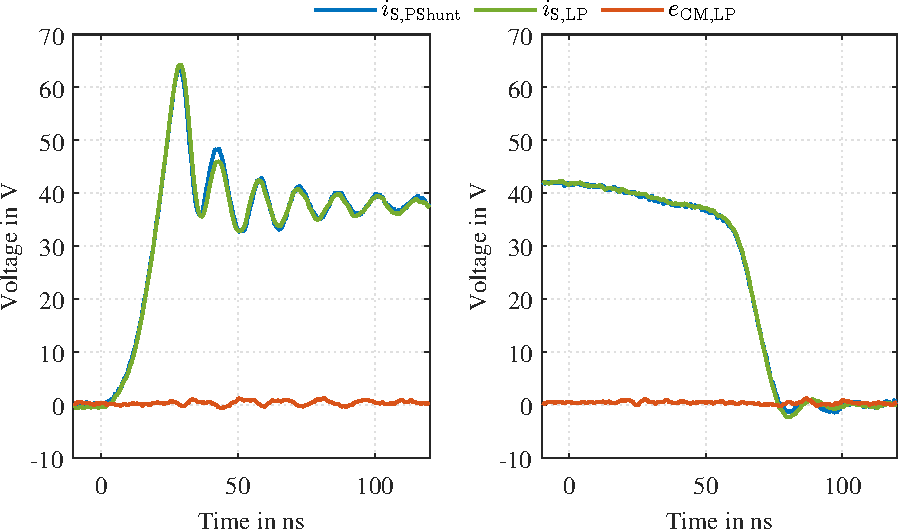
\includegraphics[scale=1]{figures/5_CurrentProbe/MS_Current_AvsPShunt_TD.pdf}
	\caption{Time-domain verification using a passive shunt.}\label{fig:MS_Current_AvsPShunt_TD}
\end{figure}

The measured waveforms show very good agreement between the active and passive shunts, both in the transient slope and in the observed overvoltage.
Only a small deviation appears in the second period of the main oscillation.
This deviation cannot be attributed to common-mode error, which is clearly much smaller.
It is therefore most likely caused by residual capacitive coupling from the voltage transient into the current shunt.


\subsection{Noise Behavior}
In a last step, the noise behavior of the active shunt is evaulated.
The measurement results are shown in \fref{fig:MS_Current_Noise}, where the noise floor of the active shunt is compared with the passive shunt.
	%!TeX root = main.tex
%!encoding = UTF-8 Unicode

\chapter{Platform for Combined Intrinsic and System-Level EMC Measurements (10-15 pages)}
\label{ch:TestBench}

The measurement setup aims to incorporate the methods discussed in the previous section to measure the EMC-relevant signal components of drain-source voltages and the drain current.
Furthermore a conventional EMC measurement through two LISNs is installed to compare the measurements results of the intrinsic EM emissions of the switch with conventional measurements.

%\section{Main Setup (different title?)}
%\subsection{Requirements}
%\subsection{Design}

A picture of the measurement setup is shown in \fref{fig:pic_b2b_setup} and its equivalent circuit is depicted in \fref{fig:ESB_b2b}.


%!TeX root = main.tex
%!encoding = UTF-8 Unicode

\section{Requirements for the Integrated EMC Measurement Environment}

The measurement platform must fulfill several requirements to enable reproducible and EMC-relevant characterization under realistic operating conditions.
First, it must provide a classical ground reference that represents the inverter chassis and allows physically meaningful coupling paths for high-frequency currents.
Second, the switching behavior of the test setup must be comparable to that of real applications, so that the measured emission spectra remain representative of practical converter operation.
Third, the platform must support the different measurement methodologies introduced in this work, in particular the operation of pulse chains with multiple consecutive switching events at a defined operating point.
Fourth, the setup must include a conducted-EMC reference measurement based on a LISN to allow direct comparison between intrinsic device emissions and standardized system-level quantities.
Fifth, additional noise sources introduced by the test environment must be minimized.
This includes filtering of the supply paths via the LISN, optical transmission of control signals, battery-powered gate-driver supplies, and a linear load implementation based on an air-core inductor.
Finally, the platform must allow stable operation during pulse-chain measurements without requiring active thermal management; therefore, passive cooling has to be sufficient for the intended operating regime.

The design choices discussed in the following section are derived directly from these requirements and are presented in the same logical order.

%!TeX root = main.tex
%!encoding = UTF-8 Unicode

\section{Design}
The two DUTs \mti{Q}{1} and \mti{Q}{2} are placed on a cooler, which is mounted on a aluminum plate, which creates the current path for the ground currents to the two LISNs.

As will be seen later, a second half-bridge with \mti{Q}{1,aux} and \mti{Q}{2,aux} is placed adjacent to the DUTs.
This half-bridge is needed, because a single double pulse test is not sufficient for EMC measurements.
Instead multiple pulses which are averaged in post-processing are needed to decrease the thermal noise.
However, the EM noise of the auxiliary half-bridge should not be seen on the LISN measurements and, hence, it is not placed on the aluminum plate.
The DC ports of the auxiliary half-bridge are additionally isolated from the DUTs through the impedance of the LISNs and of the inductor.

\begin{figure}[h]
	\centering
	\import{./figures/}{ESB_B2B.pdf_tex}
	\caption{Equivalent circuit diagram of the back-to-back converter measurement setup. Add vds and id lp hp signals}
	\label{fig:ESB_b2b}
\end{figure}

\subsection{Back-to-Back Converter}


\subsection{LISN Measurement}



xxx optionally push into measurement chapter and rename it xxx
	%!TeX root = main.tex
%!encoding = UTF-8 Unicode
\chapter{Measurement Results}

\section{Chip Size Area}
\section{Technology Comparison}
\section{Passives}

	%!TeX root = main.tex
%!encoding = UTF-8 Unicode
\chapter{Conclusion}




\appendix					%% Kapitelnumerierung mit Buchstaben
%%=============================================================================
%%=== ISEA-TEX-Vorlage ===
%%===   Verzeichnisse   ===
%%===      jmu 05.07.2012     ===
%%=============================================================================

%% Hinweis: folgende Zeilen einkommentieren, wenn ein Abkürzungsverzeichnis erwünscht ist.

%\ifthenelse{\equal{\varLanguage}{german}}
%{\printglossary[type=\acronymtype,style=long,title={Abkürzungsverzeichnis},toctitle={Abkürzungsverzeichnis}]}
%{\printglossary[type=\acronymtype,style=long,title={Glossary},toctitle={Glossary}]}


%% Hinweis: folgende Zeilen einkommentieren, wenn ein Symbolverzeichnis verwendet wird.
%\clearpage
%\ifthenelse{\equal{\varLanguage}{german}}
%{\printglossary[type=symbolslist,style=long,title={Symbolverzeichnis},toctitle={Symbolverzeichnis}]}
%{\printglossary[type=symbolslist,style=long,title={List of Symbols},toctitle={List of Symbols}]}

%% Hinweis: folgende Zeilen einkommentieren, wenn ein Fremdwortverzeichnis verwendet wird.
%\clearpage
%\ifthenelse{\equal{\varLanguage}{german}}
%{\printglossary[type=fremdwort,style=long,title={Fremdwörterverzeichnis},toctitle={Fremdwörterverzeichnis}] }
%{\printglossary[type=fremdwort,style=long,title={List of Foreign Words},toctitle={List of Foreign Words}]}
%%Fremdworte ausgeben

\listoffigures         				 	%% Abbildungsverzeichnis
\listoftables							%% Tabellenverzeichnis

%%Literaturverzeichnis	
\printbibliography[heading=bibintoc]			%% Literaturverzeichnis erstellen
%\newpage
%\printindex			%% Literaturverzeichnis, Symbolverzeichnis, Fremwortverzeichnis werden nun erzeugt

\backmatter					%% keine Kapitelnumerierung (wie bei \frontmatter)
							%% fuer Danksagung oder CV
							
							
% %%=============================================================================
%%===   ISEA-TEX-Vorlage   ===
%%=== Formblatt zur Arbeit ===
%%===        mla 2016      ===
%%=============================================================================

%%	Diese Datei braucht i.d.R. nicht editiert zu werden, es werden die Werte aus isea_tex_def übernommen.

\label{SummaryForm}

\thispagestyle{empty}
%\edef\pagenumstart{\value{page}}

\small
Diese Seite wird nicht mitgebunden und ist als separate Seite bei der Abgabe der Arbeit mit abzugeben.
%\normalsize
\vspace{5mm}

\varTitle
\vspace{5mm}

\varDate
\vspace{5mm}

Autor: \varAuthorFamily{}, \varAuthorGiven{}

Betreuende/r Mitarbeiter/in: \varAssiName

Betreuender Professor: \varSupA

\vspace{5mm}
\ifthenelse{\equal{\varInstitute}{ISEA}}
{
	Arbeit außerhalb des ISEA angefertigt: \textbf{\ifthenelse{\equal{\varExtern}{true}}{ja}{nein}}
}
{
	Arbeit außerhalb des PGS angefertigt: \textbf{\ifthenelse{\equal{\varExtern}{true}}{ja}{nein}}
}

\ifthenelse{\equal{\varExtern}{true}}
{
	Firma der Anfertigung: \varExternName
}
{}

\vspace{5mm}

Studienrichtung: \varFieldOfStudy

Sprache: \ifthenelse{\equal{\varLanguage}{german}}{Deutsch}{Englisch}

\vspace{7mm}
Vertraulichkeit:

\ifthenelse{\equal{\varInstitute}{ISEA}}
{
	$\square$ Diese Arbeit fällt unter eine Geheimhaltungsvereinbarung des ISEAs und beinhaltet vertrauliche Daten.
}
{
	$\square$ Diese Arbeit fällt unter eine Geheimhaltungsvereinbarung des PGS und beinhaltet vertrauliche Daten.	
}

$\square$ Diese Arbeit steht unter erweiterten Geheimhaltungsvereinbarungen mit Dritten oder zum Schutz von Erfindungsrechten.

$\square$ Diese Arbeit hat einen Sperrvermerk bis zum \ldots \ldots \ldots .

\vspace{5mm}

Stichworte:
\begin{multicols}{2}
	\begin{itemize}
		\itemsep 0pt
		\makeatletter
		\@for\tmp:=\varKeywords\do{\item \tmp}
		\makeatother
	\end{itemize}
\end{multicols}


\vspace{5mm}

Zusammenfassung:


Hier steht eine kurze Zusammenfassung der Arbeit. Der Umfang der Zusammenfassung sollte vier bis acht Zeilen betragen.

Dieser Text ist in der Datei \textbf{SummaryForm.tex} zu finden, weitere Parameter (Betreuer, Studienrichtung, ...) können entweder in der \textbf{isea\_tex\_def.tex} oder direkt in dieser Datei angepasst werden.


\cleardoubleemptypage
\normalsize
%\setcounter{page}{\pagenumstart-1}	% Zähler zurücksetzen, als ob Seite nicht vorhanden wäre
		%% Formblatt, welches separat abzugeben ist.
% %%=============================================================================
%%===   ISEA-TEX-Vorlage   ===
%%=== Erklärung des Autors ===
%%===       mla 2016       ===
%%=============================================================================

% disable externalize for this page if it was enabled in isea_tex_def (prevents compilation errors)
\ifdef{\tikzexternaldisable}{
	\tikzexternaldisable
}{}

\includepdf[pagecommand={
	\begin{tikzpicture}[
		remember picture,
		overlay,
		shift={(current page.south west)}
	]	
		\sffamily
		\bfseries
		\node[anchor=south west] at (24mm, 239mm) {\varAuthorFamily{}, \varAuthorGiven{}};
		\node[anchor=north west, text width=160mm] at (24mm, 214mm) {\baselineskip=19.5pt \varTitle{} \\ };
		\node[anchor=south west] at (24mm, 141.5mm) {Aachen, \varDate{}};
		\node[anchor=south west] at (24mm, 30.8mm) {Aachen, \varDate{}};
		\normalfont
	\end{tikzpicture}
	\thispagestyle{empty}
}]{eidesstattlicheVersicherung}

\cleardoubleemptypage

\ifdef{\tikzexternalenable}{
	\tikzexternalenable
}{}

		%% Eidesstattliche Versicherung, wird ebenfalls separat abgegeben

\end{document}



